\DocumentMetadata{%
 %  uncompress, %only for debugging!!
  pdfversion=2.0,
  testphase={phase-II, tabular, graphic}%
 % testphase={phase-II,math, tabular, graphic}% TOC Does not work
   % testphase={phase-III,math}% TOC works
}
\tagpdfsetup{activate, tabsorder=structure}
% Use the following to fix bug in November 2023 download of LaTeX
\ExplSyntaxOn
\cs_generate_variant:Nn\__tag_prop_gput:Nnn{cnx}
\ExplSyntaxOff
\documentclass[11pt,
  english,
  letterpaper,
]{article}
\usepackage{sa4ss}
\usepackage{amsmath,amssymb,array}
\usepackage{booktabs}

% From tagged-template.latex
\usepackage{lmodern}
\usepackage{ifxetex,ifluatex}
\ifnum 0\ifxetex 1\fi\ifluatex 1\fi=0 % if pdftex
  \usepackage[T1]{fontenc}
  \usepackage[utf8]{inputenc}
  \usepackage{textcomp} % provide euro and other symbols
\else % if luatex or xetex
  \usepackage{unicode-math}
  \defaultfontfeatures{Scale=MatchLowercase}
  \defaultfontfeatures[\rmfamily]{Ligatures=TeX,Scale=1}
\fi

% Use upquote if available, for straight quotes in verbatim environments
\IfFileExists{upquote.sty}{\usepackage{upquote}}{}
\IfFileExists{microtype.sty}{% use microtype if available
  \usepackage[]{microtype}
  \UseMicrotypeSet[protrusion]{basicmath} % disable protrusion for tt fonts
}{}
\makeatletter
\@ifundefined{KOMAClassName}{% if non-KOMA class
  \IfFileExists{parskip.sty}{%
    \usepackage{parskip}
  }{% else
    \setlength{\parindent}{0pt}
    \setlength{\parskip}{6pt plus 2pt minus 1pt}}
}{% if KOMA class
  \KOMAoptions{parskip=half}}
\makeatother
\usepackage{xcolor}
\IfFileExists{xurl.sty}{\usepackage{xurl}}{} % add URL line breaks if available
\hypersetup{
  pdftitle={Status of copper rockfish (Sebastes caurinus) along the U.S. California coast south of Point Conception in 2023},
  pdflang={en},
  hidelinks,
  pdfcreator={LaTeX via pandoc}}
\urlstyle{same} % disable monospaced font for URLs
\usepackage{longtable}
% Correct order of tables after \paragraph or \subparagraph
\usepackage{etoolbox}
\makeatletter
\patchcmd\longtable{\par}{\if@noskipsec\mbox{}\fi\par}{}{}
\makeatother
% Allow footnotes in longtable head/foot
\IfFileExists{footnotehyper.sty}{\usepackage{footnotehyper}}{\usepackage{footnote}}
\makesavenoteenv{longtable}
\usepackage{graphicx}
\makeatletter
\def\maxwidth{\ifdim\Gin@nat@width>\linewidth\linewidth\else\Gin@nat@width\fi}
\def\maxheight{\ifdim\Gin@nat@height>\textheight\textheight\else\Gin@nat@height\fi}
\makeatother
% Scale images if necessary, so that they will not overflow the page
% margins by default, and it is still possible to overwrite the defaults
% using explicit options in \includegraphics[width, height, ...]{}
\setkeys{Gin}{width=\maxwidth,height=\maxheight,keepaspectratio}
% Set default figure placement to htbp
\makeatletter
\def\fps@figure{htbp}
\makeatother
\setlength{\emergencystretch}{3em} % prevent overfull lines
\providecommand{\tightlist}{%
  \setlength{\itemsep}{0pt}\setlength{\parskip}{0pt}}
\setcounter{secnumdepth}{5}
\usepackage{lineno}
\usepackage[inline]{showlabels}
\ifxetex
  % Load polyglossia as late as possible: uses bidi with RTL langages (e.g. Hebrew, Arabic)
  \usepackage{polyglossia}
  \setmainlanguage[]{}
\else
  \usepackage[shorthands=off,main=english]{babel}
\fi

%Define cslreferences environment, required by pandoc 2.8
%https://github.com/rstudio/rmarkdown/issues/1649
\newlength{\csllabelwidth}
\setlength{\csllabelwidth}{3em}
\newlength{\cslhangindent}
\setlength{\cslhangindent}{1.5em}
% for Pandoc 2.8 to 2.10.1
\newenvironment{cslreferences}%
  {}%
  {\par}
% For Pandoc 2.11+
\newenvironment{CSLReferences}[2] % #1 hanging-ident, #2 entry spacing
 {% don't indent paragraphs
  \setlength{\parindent}{0pt}
  % turn on hanging indent if param 1 is 1
  \ifodd #1 \everypar{\setlength{\hangindent}{\cslhangindent}}\ignorespaces\fi
  % set entry spacing
  \ifnum #2 > 0
  \setlength{\parskip}{#2\baselineskip}
  \fi
 }%
 {}
\usepackage{calc}  % for \widthof, \maxof in minipage
\newcommand{\CSLBlock}[1]{#1\hfill\break}
\newcommand{\CSLLeftMargin}[1]{\parbox[t]{\csllabelwidth}{#1}}
\newcommand{\CSLRightInline}[1]{\parbox[t]{\linewidth - \csllabelwidth}{#1}\break}
\newcommand{\CSLIndent}[1]{\hspace{\cslhangindent}#1}


\providecommand{\tightlist}{%
  \setlength{\itemsep}{0pt}\setlength{\parskip}{0pt}}

\usepackage{lineno}
\usepackage[inline]{showlabels}
\date{}
\newcommand{\trTitle}{Status of copper rockfish (\emph{Sebastes caurinus}) along the U.S. California coast south of Point Conception in 2023}
\newcommand{\trYear}{2023}
\newcommand{\trMonth}{May}
\newcommand{\trAuthsLong}{truetruetrue}
\newcommand{\trAuthsBack}{Wetzel, C.R., M.H. Monk, J. Coates}
\newcommand{\trCitation}{
\begin{hangparas}{1em}{1}
\trAuthsBack{}. \trYear{}. \trTitle{}. \glsentrylong{pfmc}, Portland, Oregon. \pageref{LastPage}{}\,p.
\end{hangparas}}

\newcommand\includegraphicsifexists[2][width=\linewidth]{\IfFileExists{#2}{\includegraphics[#1]{#2}}{}}

\begin{document}

%%%%% Frontmatter %%%%%

% Footnote symbols in front matter
\renewcommand*{\thefootnote}{\fnsymbol{footnote}}

\small
\thispagestyle{empty}
\pagenumbering{roman}
\noindent
\begin{center}
\title{Status of copper rockfish (\emph{Sebastes caurinus}) along the U.S. California coast south of Point Conception in 2023}
% \textnormal{\MakeTextUppercase{\trTitle{}}}
\vspace{1.5cm}
{\Large\textbf\newline{Status of copper rockfish (\emph{Sebastes caurinus}) along the U.S. California coast south of Point Conception in 2023}}

\includegraphicsifexists[width=4in]{figure_title.png}
\vfill
by\\
Chantel R. Wetzel\textsuperscript{1}\\
Melissa H. Monk\textsuperscript{2}\\
Julia Coates\textsuperscript{3}\vfill
\textsuperscript{1}Northwest Fisheries Science Center, U.S. Department of Commerce, National Oceanic and Atmospheric Administration, National Marine Fisheries Service, 2725 Montlake Boulevard East, Seattle, Washington 98112\\
\textsuperscript{2}Southwest Fisheries Science Center, U.S. Department of Commerce, National Oceanic and Atmospheric Administration, National Marine Fisheries Service, 110 McAllister Way, Santa Cruz, California 95060\\
\textsuperscript{3}California Department of Fish and Wildlife, Marine Region 1933 Cliff Drive, Suite 9, Santa Barbara, California 93109\vfill
\trMonth{} \trYear{}
\end{center}
\clearpage

% Fourth page: Colophon
\thispagestyle{empty}
\vspace*{\fill}
\begin{center}
\copyright{} \glsentrylong{pfmc}, \trYear{}\\
\end{center}
\par
\bigskip
\noindent
Correct citation for this publication:
\bigskip
\par
\trCitation{}
\clearpage

% Add TOC to pdf bookmarks (clickable pdf)
\pdfbookmark[1]{\contentsname}{toc}

% Table of contents page, lists of figures and tables
\tableofcontents\clearpage
\label{TRlastRoman}
\clearpage

% Table of contents
\newpage
\thispagestyle{empty} % to remove page number

% Settings for the main document
\pagenumbering{arabic}  % Regular page numbers
\pagestyle{plain}  % No page number on first page of main document, use 'empty'
\renewcommand*{\thefootnote}{\arabic{footnote}}  % Back to numeric footnotes
\setcounter{footnote}{0}  % And start at 1
\renewcommand{\headrulewidth}{0.5pt}
\renewcommand{\footrulewidth}{0.5pt}
%\pagestyle{fancy}\fancyhead[c]{Draft: Do not cite or circulate}

\newcommand{\lt}{\ensuremath <}
\newcommand{\gt}{\ensuremath >}

\linenumbers

\newcommand\CapeM{$40^\circ 10^\prime$ N. lat.}
\newcommand\PtC{$34^\circ 27^\prime$ N. lat.}
\newcommand\CAOR{$42^\circ 00^\prime$ N. lat.}

\pagebreak
\pagenumbering{roman}
\setcounter{page}{1}

\renewcommand{\thetable}{\roman{table}}
\renewcommand{\thefigure}{\roman{figure}}

\setlength\parskip{0.5em plus 0.1em minus 0.2em}

\vspace{500cm}

\hypertarget{disclaimer}{%
\section*{Disclaimer}\label{disclaimer}}
\addcontentsline{toc}{section}{Disclaimer}

\emph{\textbf{These materials do not constitute a formal publication and are for information only. They are in a pre-review, pre-decisional state and should not be formally cited or reproduced. They are to be considered provisional and do not represent any determination or policy of NOAA or the Department of Commerce.}}

\pagebreak

\hypertarget{executive-summary}{%
\section*{Executive summary}\label{executive-summary}}
\addcontentsline{toc}{section}{Executive summary}

\hypertarget{stock}{%
\subsection*{Stock}\label{stock}}
\addcontentsline{toc}{subsection}{Stock}

This assessment reports the status of copper rockfish (\emph{Sebastes caurinus}) off the California coast in U.S. waters, using data through 2022. The copper rockfish stock was assessed using two sub-area models that captured distinct inter-stock dynamics split north and south of Point Conception. The estimated dynamics for each assessed sub-area is described here along with the combined stock status for the California stock. This assessment does not account for populations located in Mexico waters or other areas off the U.S. coast and assumes that these southern and northern populations do not contribute to the population being assessed here.

\hypertarget{catches}{%
\subsection*{Catches}\label{catches}}
\addcontentsline{toc}{subsection}{Catches}

Replace text with trends and current levels. Include Table for last 10 years. Include Figure with long-term estimates.

\begingroup\fontsize{10}{12}\selectfont
\begingroup\fontsize{10}{12}\selectfont

\begin{longtable}[t]{r>{\centering\arraybackslash}p{1.83cm}>{\centering\arraybackslash}p{1.83cm}>{\centering\arraybackslash}p{1.83cm}>{\centering\arraybackslash}p{1.83cm}>{\centering\arraybackslash}p{1.83cm}}
\caption{\label{tab:south-removalsES}Recent catch by fleet and total catch summed across fleets for the sub-area model south of Point Conception.}\\
\toprule
Year & Commercial dead & Commercial live & Rec CPFV & Rec Private & Total Catch\\
\midrule
\endfirsthead
\caption[]{Recent catch by fleet and total catch summed across fleets for the sub-area model south of Point Conception. \textit{(continued)}}\\
\toprule
Year & Commercial dead & Commercial live & Rec CPFV & Rec Private & Total Catch\\
\midrule
\endhead

\endfoot
\bottomrule
\endlastfoot
2013 & 1.26 & 2.67 & 61.65 & 13.96 & 79.54\\
2014 & 1.79 & 2.29 & 47.58 & 10.04 & 61.71\\
2015 & 2.11 & 4.09 & 67.00 & 8.97 & 82.18\\
2016 & 2.11 & 3.57 & 82.20 & 11.07 & 98.95\\
2017 & 1.74 & 2.82 & 70.58 & 11.72 & 86.86\\
2018 & 2.93 & 2.20 & 81.97 & 14.21 & 101.31\\
2019 & 2.71 & 3.08 & 60.25 & 14.66 & 80.70\\
2020 & 3.54 & 3.58 & 56.39 & 23.01 & 86.52\\
2021 & 2.74 & 1.94 & 44.25 & 8.28 & 57.20\\
2022 & 0.69 & 0.21 & 14.12 & 4.50 & 19.52\\*
\end{longtable}
\endgroup{}
\endgroup{}


\begingroup\fontsize{10}{12}\selectfont
\begingroup\fontsize{10}{12}\selectfont

\begin{table}[t]{r>{\centering\arraybackslash}p{1.83cm}>{\centering\arraybackslash}p{1.83cm}>{\centering\arraybackslash}p{1.83cm}>{\centering\arraybackslash}p{1.83cm}>{\centering\arraybackslash}p{1.83cm}}
\caption{\label{tab:north-removalsES}Recent catches (mt) by fleet and total catch (mt) summed across fleets for the sub-area model north of Point Conception.}\\
\toprule
Year & Commercial Dead & Commercial Live & Rec CPFV & Rec PR & Total Catch\\
\midrule
\endfirsthead
\caption[]{Recent catches (mt) by fleet and total catch (mt) summed across fleets for the sub-area model north of Point Conception. \textit{(continued)}}\\
\toprule
Year & Commercial Dead & Commercial Live & Rec CPFV & Rec PR & Total Catch\\
\midrule
\endhead

\endfoot
\bottomrule
\endlastfoot
2013 & 0.70 & 2.11 & 8.83 & 14.00 & 25.64\\
2014 & 0.74 & 2.47 & 16.10 & 17.63 & 36.94\\
2015 & 0.78 & 2.69 & 24.22 & 37.77 & 65.46\\
2016 & 0.83 & 2.57 & 28.69 & 34.23 & 66.32\\
2017 & 1.41 & 4.60 & 56.48 & 76.13 & 138.62\\
2018 & 3.04 & 6.36 & 43.97 & 49.01 & 102.38\\
2019 & 2.49 & 6.85 & 39.16 & 53.39 & 101.89\\
2020 & 3.90 & 7.55 & 36.55 & 55.17 & 103.17\\
2021 & 3.10 & 7.55 & 24.98 & 41.42 & 77.05\\
2022 & 1.19 & 1.92 & 11.50 & 32.53 & 47.15\\
\end{table}
\endgroup{}
\endgroup{}


\begin{figure}
\centering
\includegraphics[width=1\textwidth,height=1\textheight]{N:/Assessments/CurrentAssessments/copper_rockfish_2023/models/sca/14.0_base_forecast/plots/catch2 landings stacked.png}
\caption{Landings by fleet used in the base model for the area south of Point Conception where catches in metric tons by fleet are stacked.\label{fig:es-south-catch}}
\end{figure}

\begin{figure}
\centering
\includegraphics[width=1\textwidth,height=1\textheight]{N:/Assessments/CurrentAssessments/copper_rockfish_2023/models/nca/9.8_selex_fix_forecast/plots/catch2 landings stacked.png}
\caption{Landings by fleet used in the base model for the area north of Point Conception where catches in metric tons by fleet are stacked.\label{fig:es-north-catch}}
\end{figure}

\hypertarget{data-and-assessment}{%
\subsection*{Data and assessment}\label{data-and-assessment}}
\addcontentsline{toc}{subsection}{Data and assessment}

This assessment uses the stock assessment framework Stock Synthesis version 3.30.21 (SS3).

Replace text with date of last assessment, type of assessment model, data available, new information, and information lacking.

\hypertarget{stock-biomass-and-dynamics}{%
\subsection*{Stock biomass and dynamics}\label{stock-biomass-and-dynamics}}
\addcontentsline{toc}{subsection}{Stock biomass and dynamics}

Replace text with trends and current levels relative to virgin or historic levels and description of uncertainty. Include Table for last 10 years. Include Figure with long-term estimates.

\begingroup\fontsize{10}{12}\selectfont
\begingroup\fontsize{10}{12}\selectfont

\begin{longtable}[t]{r>{\centering\arraybackslash}p{1.57cm}>{\centering\arraybackslash}p{1.57cm}>{\centering\arraybackslash}p{1.57cm}>{\centering\arraybackslash}p{1.57cm}>{\centering\arraybackslash}p{1.57cm}>{\centering\arraybackslash}p{1.57cm}}
\caption{\label{tab:south-ssbES}Estimated recent trend in spawning output and the fraction unfished and the 95 percent intervals for the sub-area model south of Point Conception.}\\
\toprule
Year & Spawning Output & Lower Interval & Upper Interval & Fraction Unfished & Lower Interval & Upper Interval\\
\midrule
\endfirsthead
\caption[]{Estimated recent trend in spawning output and the fraction unfished and the 95 percent intervals for the sub-area model south of Point Conception. \textit{(continued)}}\\
\toprule
Year & Spawning Output & Lower Interval & Upper Interval & Fraction Unfished & Lower Interval & Upper Interval\\
\midrule
\endhead

\endfoot
\bottomrule
\endlastfoot
2013 & 29.22 & 21.10 & 37.34 & 0.14 & 0.10 & 0.19\\
2014 & 30.05 & 21.41 & 38.69 & 0.15 & 0.10 & 0.20\\
2015 & 33.46 & 23.92 & 43.00 & 0.17 & 0.11 & 0.22\\
2016 & 36.13 & 25.51 & 46.75 & 0.18 & 0.12 & 0.24\\
2017 & 37.56 & 25.74 & 49.38 & 0.19 & 0.12 & 0.25\\
2018 & 39.23 & 26.06 & 52.40 & 0.19 & 0.12 & 0.26\\
2019 & 37.92 & 23.46 & 52.38 & 0.19 & 0.11 & 0.26\\
2020 & 35.69 & 20.06 & 51.32 & 0.18 & 0.10 & 0.26\\
2021 & 32.45 & 15.87 & 49.03 & 0.16 & 0.08 & 0.24\\
2022 & 30.24 & 12.91 & 47.57 & 0.15 & 0.06 & 0.24\\
2023 & 29.76 & 11.87 & 47.65 & 0.15 & 0.06 & 0.24\\*
\end{longtable}
\endgroup{}
\endgroup{}


\begingroup\fontsize{10}{12}\selectfont
\begingroup\fontsize{10}{12}\selectfont

\begin{longtable}[t]{r>{\centering\arraybackslash}p{1.57cm}>{\centering\arraybackslash}p{1.57cm}>{\centering\arraybackslash}p{1.57cm}>{\centering\arraybackslash}p{1.57cm}>{\centering\arraybackslash}p{1.57cm}>{\centering\arraybackslash}p{1.57cm}}
\caption{\label{tab:north-ssbES}Estimated recent trend in spawning output and the fraction unfished and the 95 percent intervals for the sub-area model north of Point Conception.}\\
\toprule
Year & Spawning Output & Lower Interval & Upper Interval & Fraction Unfished & Lower Interval & Upper Interval\\
\midrule
\endfirsthead
\caption[]{Estimated recent trend in spawning output and the fraction unfished and the 95 percent intervals for the sub-area model north of Point Conception. \textit{(continued)}}\\
\toprule
Year & Spawning Output & Lower Interval & Upper Interval & Fraction Unfished & Lower Interval & Upper Interval\\
\midrule
\endhead

\endfoot
\bottomrule
\endlastfoot
2013 & 170.30 & 94.03  & 246.57 & 0.36 & 0.24 & 0.48\\
2014 & 181.67 & 100.89 & 262.44 & 0.38 & 0.25 & 0.51\\
2015 & 194.73 & 108.27 & 281.19 & 0.41 & 0.27 & 0.55\\
2016 & 205.67 & 113.14 & 298.19 & 0.43 & 0.29 & 0.58\\
2017 & 215.64 & 117.05 & 314.23 & 0.45 & 0.30 & 0.61\\
2018 & 217.87 & 113.23 & 322.51 & 0.46 & 0.29 & 0.63\\
2019 & 223.06 & 112.30 & 333.82 & 0.47 & 0.29 & 0.65\\
2020 & 227.81 & 111.02 & 344.59 & 0.48 & 0.29 & 0.67\\
2021 & 231.68 & 109.06 & 354.31 & 0.49 & 0.29 & 0.69\\
2022 & 237.18 & 108.72 & 365.64 & 0.50 & 0.29 & 0.71\\
2023 & 246.82 & 112.22 & 381.43 & 0.52 & 0.30 & 0.74\\*
\end{longtable}
\endgroup{}
\endgroup{}


\begingroup\fontsize{10}{12}\selectfont
\begingroup\fontsize{10}{12}\selectfont

\begin{longtable}[t]{c>{\centering\arraybackslash}p{1.83cm}>{\centering\arraybackslash}p{1.83cm}>{\centering\arraybackslash}p{1.83cm}>{\centering\arraybackslash}p{1.83cm}>{\centering\arraybackslash}p{1.83cm}}
\caption{\label{tab:ca-status}The estimated total biomass (mt), total biomass age 3+ (mt), age-0 recruits, spawning ouput in number of million eggs across California and fraction unfished by year.}\\
\toprule
Year & Total Biomass (mt) & Total Biomass 3+ (mt) & Age-0 Recruits & Spawning Output & Fraction Unfished\\
\midrule
\endfirsthead
\caption[]{\label{tab:ca-status}The estimated total biomass (mt), total biomass age 3+ (mt), age-0 recruits, spawning ouput in number of million eggs across California and fraction unfished by year. \textit{(continued)}}\\
\toprule
Year & Total Biomass (mt) & Total Biomass 3+ (mt) & Age-0 Recruits & Spawning Output & Fraction Unfished\\
\midrule
\endhead

\endfoot
\bottomrule
\endlastfoot
2013 & 2627.91 & 2588.61 & 928.75 & 210.14 & 0.306\\
2014 & 2795.04 & 2739.48 & 244.85 & 223.28 & 0.325\\
2015 & 2973.06 & 2916.90 & 102.22 & 240.91 & 0.350\\
2016 & 3097.56 & 3064.44 & 245.60 & 255.75 & 0.372\\
2017 & 3182.40 & 3150.11 & 122.12 & 268.46 & 0.390\\
2018 & 3182.40 & 3153.24 & 96.39 & 273.80 & 0.398\\
2019 & 3176.81 & 3131.98 & 112.02 & 279.23 & 0.406\\
2020 & 3179.52 & 3148.18 & 163.48 & 283.32 & 0.412\\
2021 & 3110.47 & 3087.05 & 317.57 & 278.75 & 0.405\\
2022 & 3108.97 & 3077.18 & 302.69 & 279.64 & 0.407\\
2023 & 3199.84 & 3163.70 & 299.87 & 289.74 & 0.421\\*
\end{longtable}
\endgroup{}
\endgroup{}

\begin{figure}
\centering
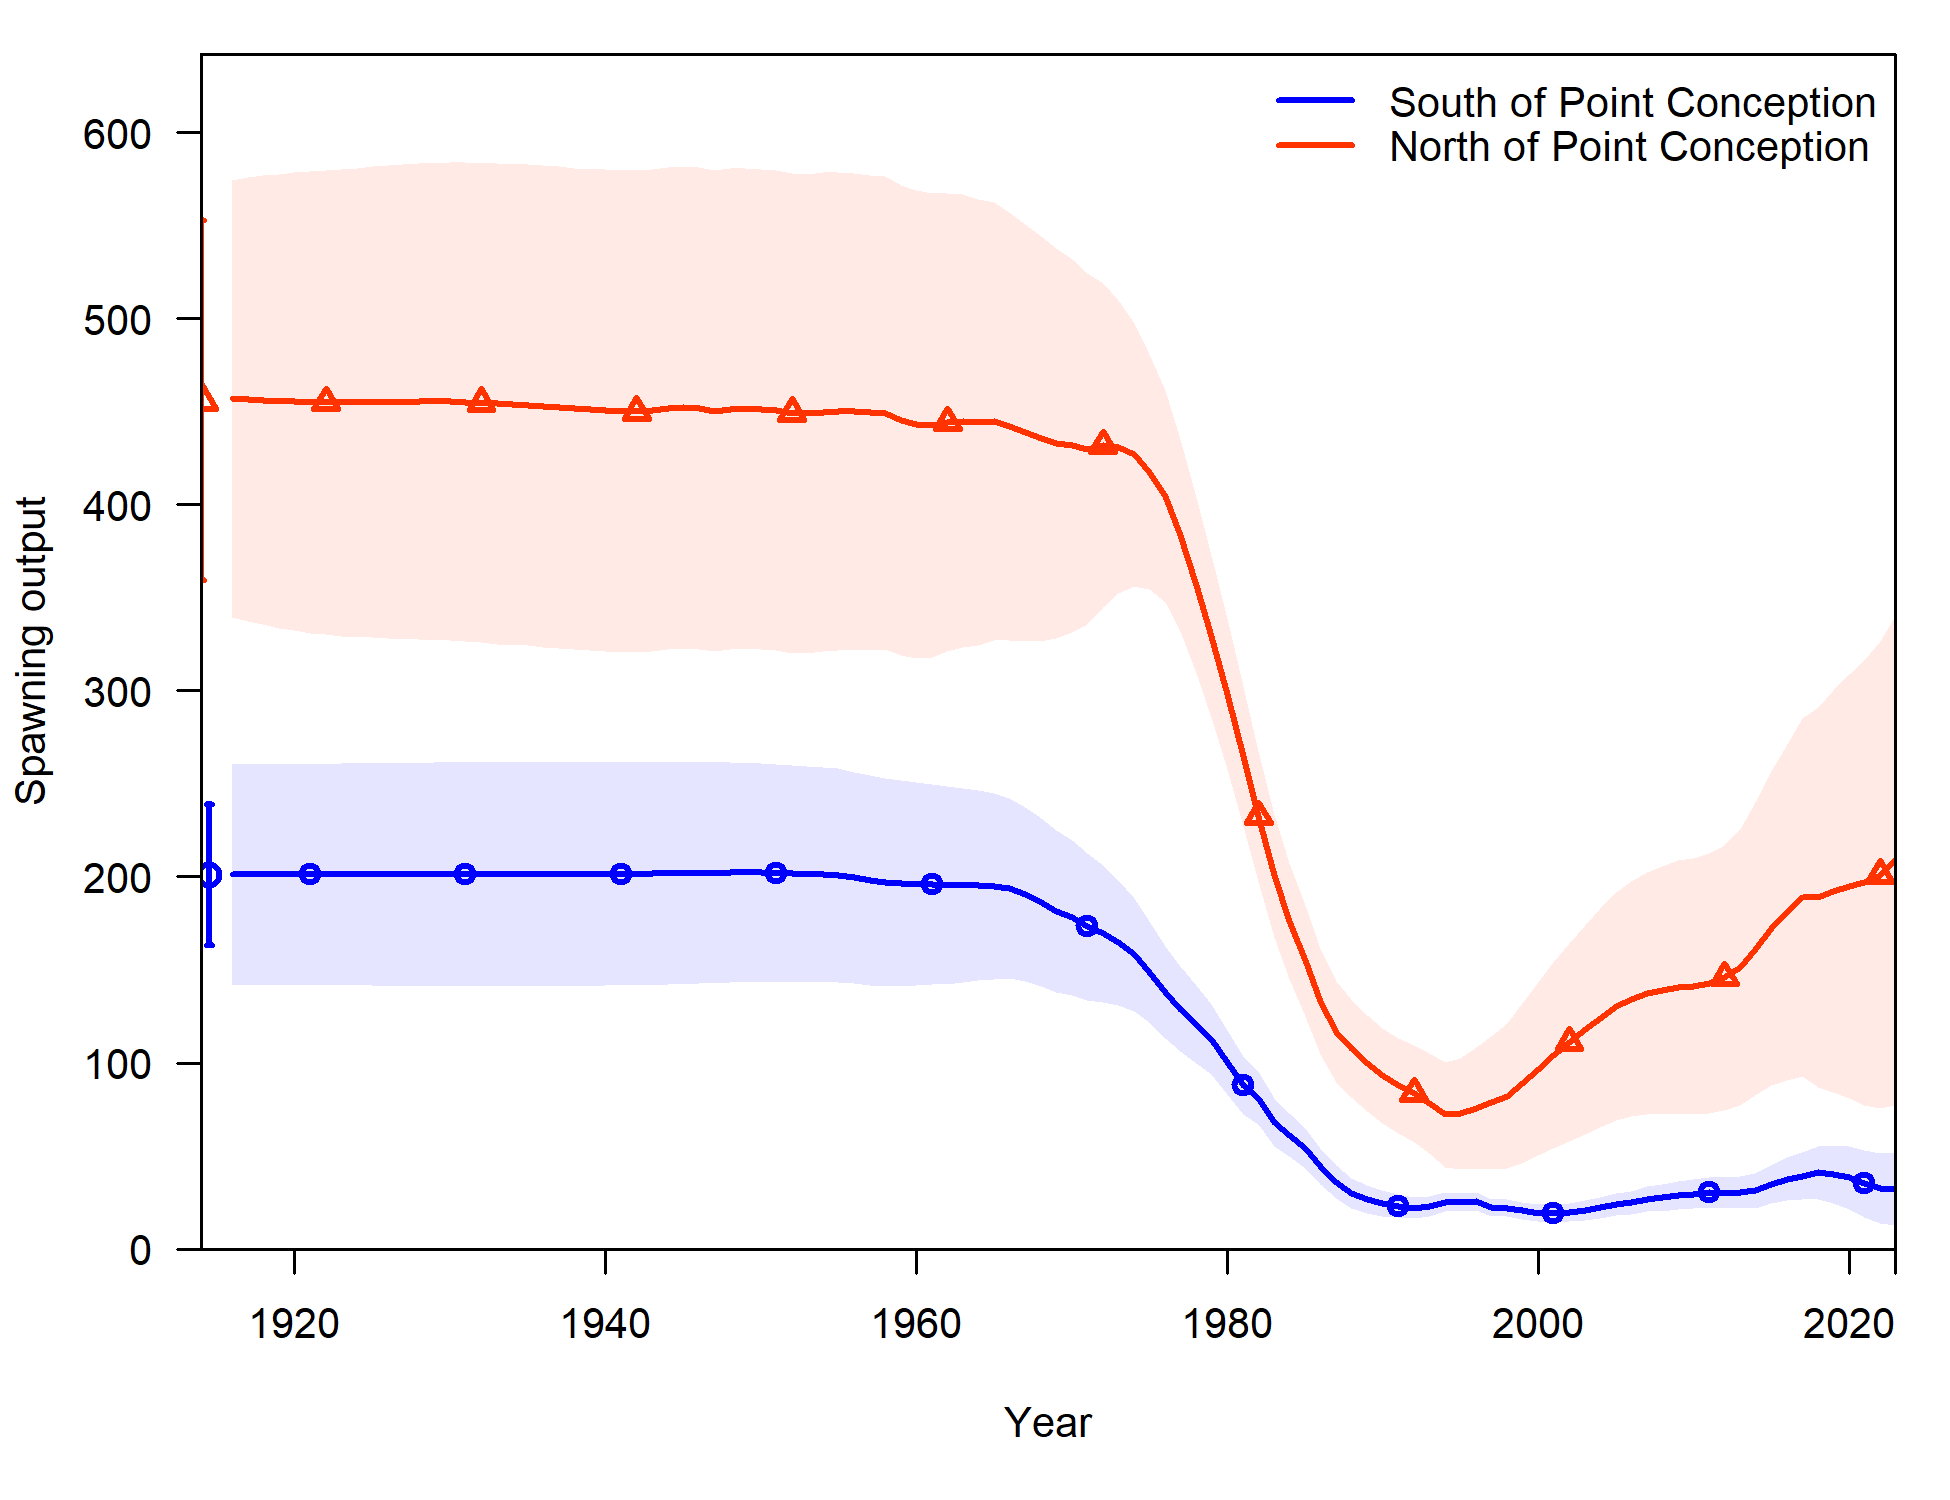
\includegraphics[width=1\textwidth,height=1\textheight]{C:/Assessments/2023/copper_rockfish_2023/documents/shared_figures/compare2_spawnbio_uncertainty.png}
\caption{Estimated time series of spawning output (circles and line: median; light broken lines: 95 percent intervals) for the model areas south and north of Point Conception.\label{fig:es-sb}}
\end{figure}

\begin{figure}
\centering
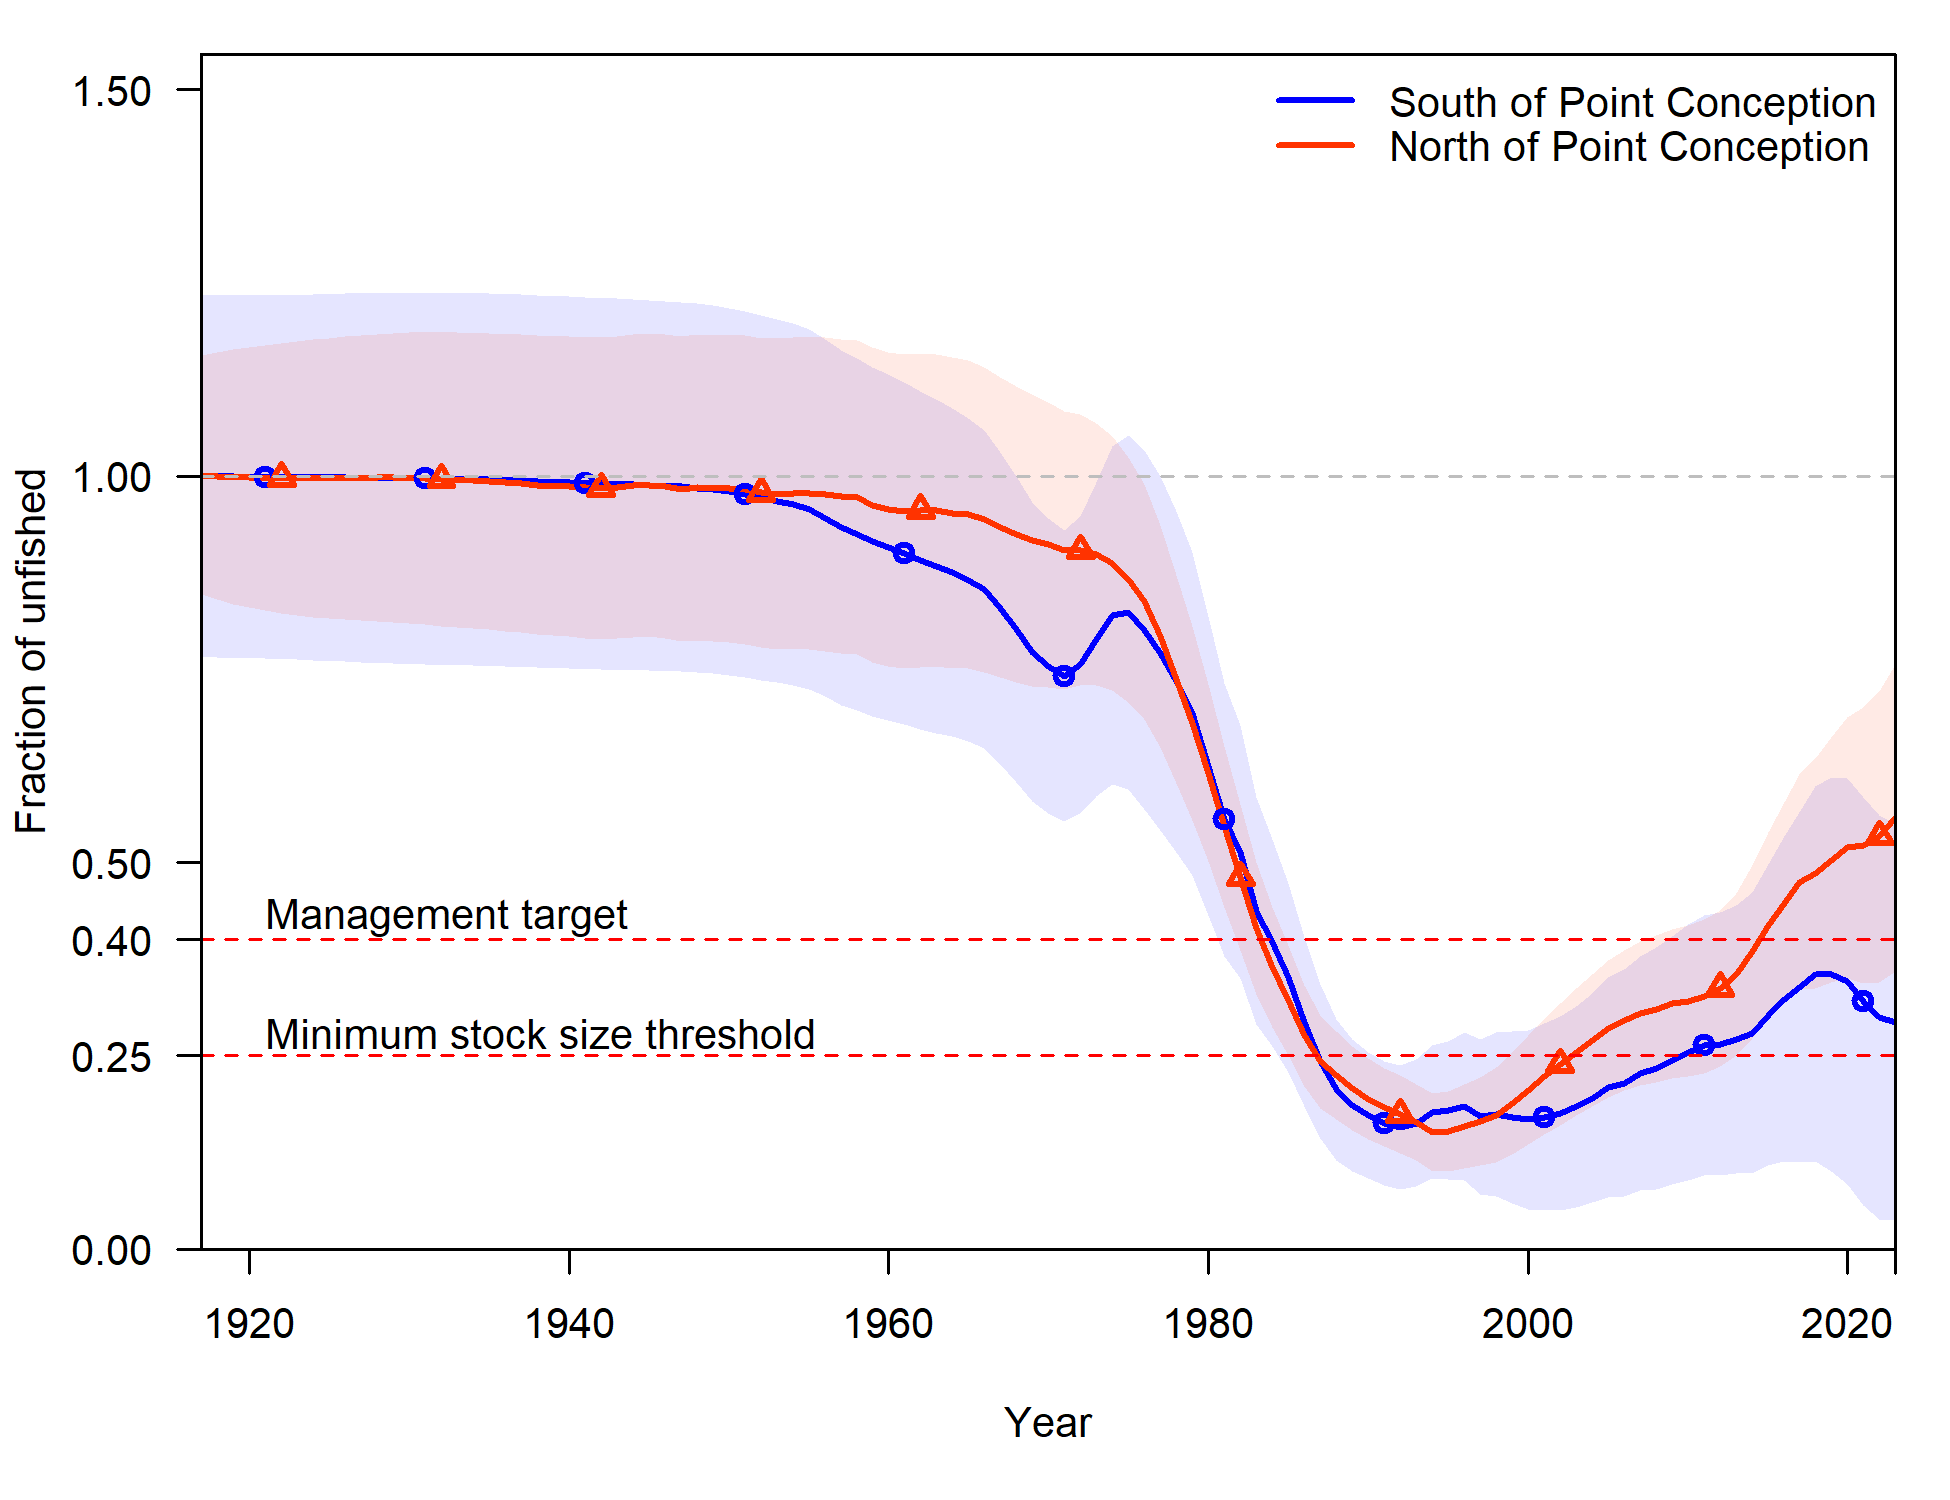
\includegraphics[width=1\textwidth,height=1\textheight]{C:/Assessments/2023/copper_rockfish_2023/documents/shared_figures/compare4_Bratio_uncertainty.png}
\caption{Estimated time series of fraction of relative spawning output (circles and line: median; light broken lines: 95 percent intervals) for the model areas south and north of Point Conception.\label{fig:es-depl}}
\end{figure}

\begin{figure}
\centering
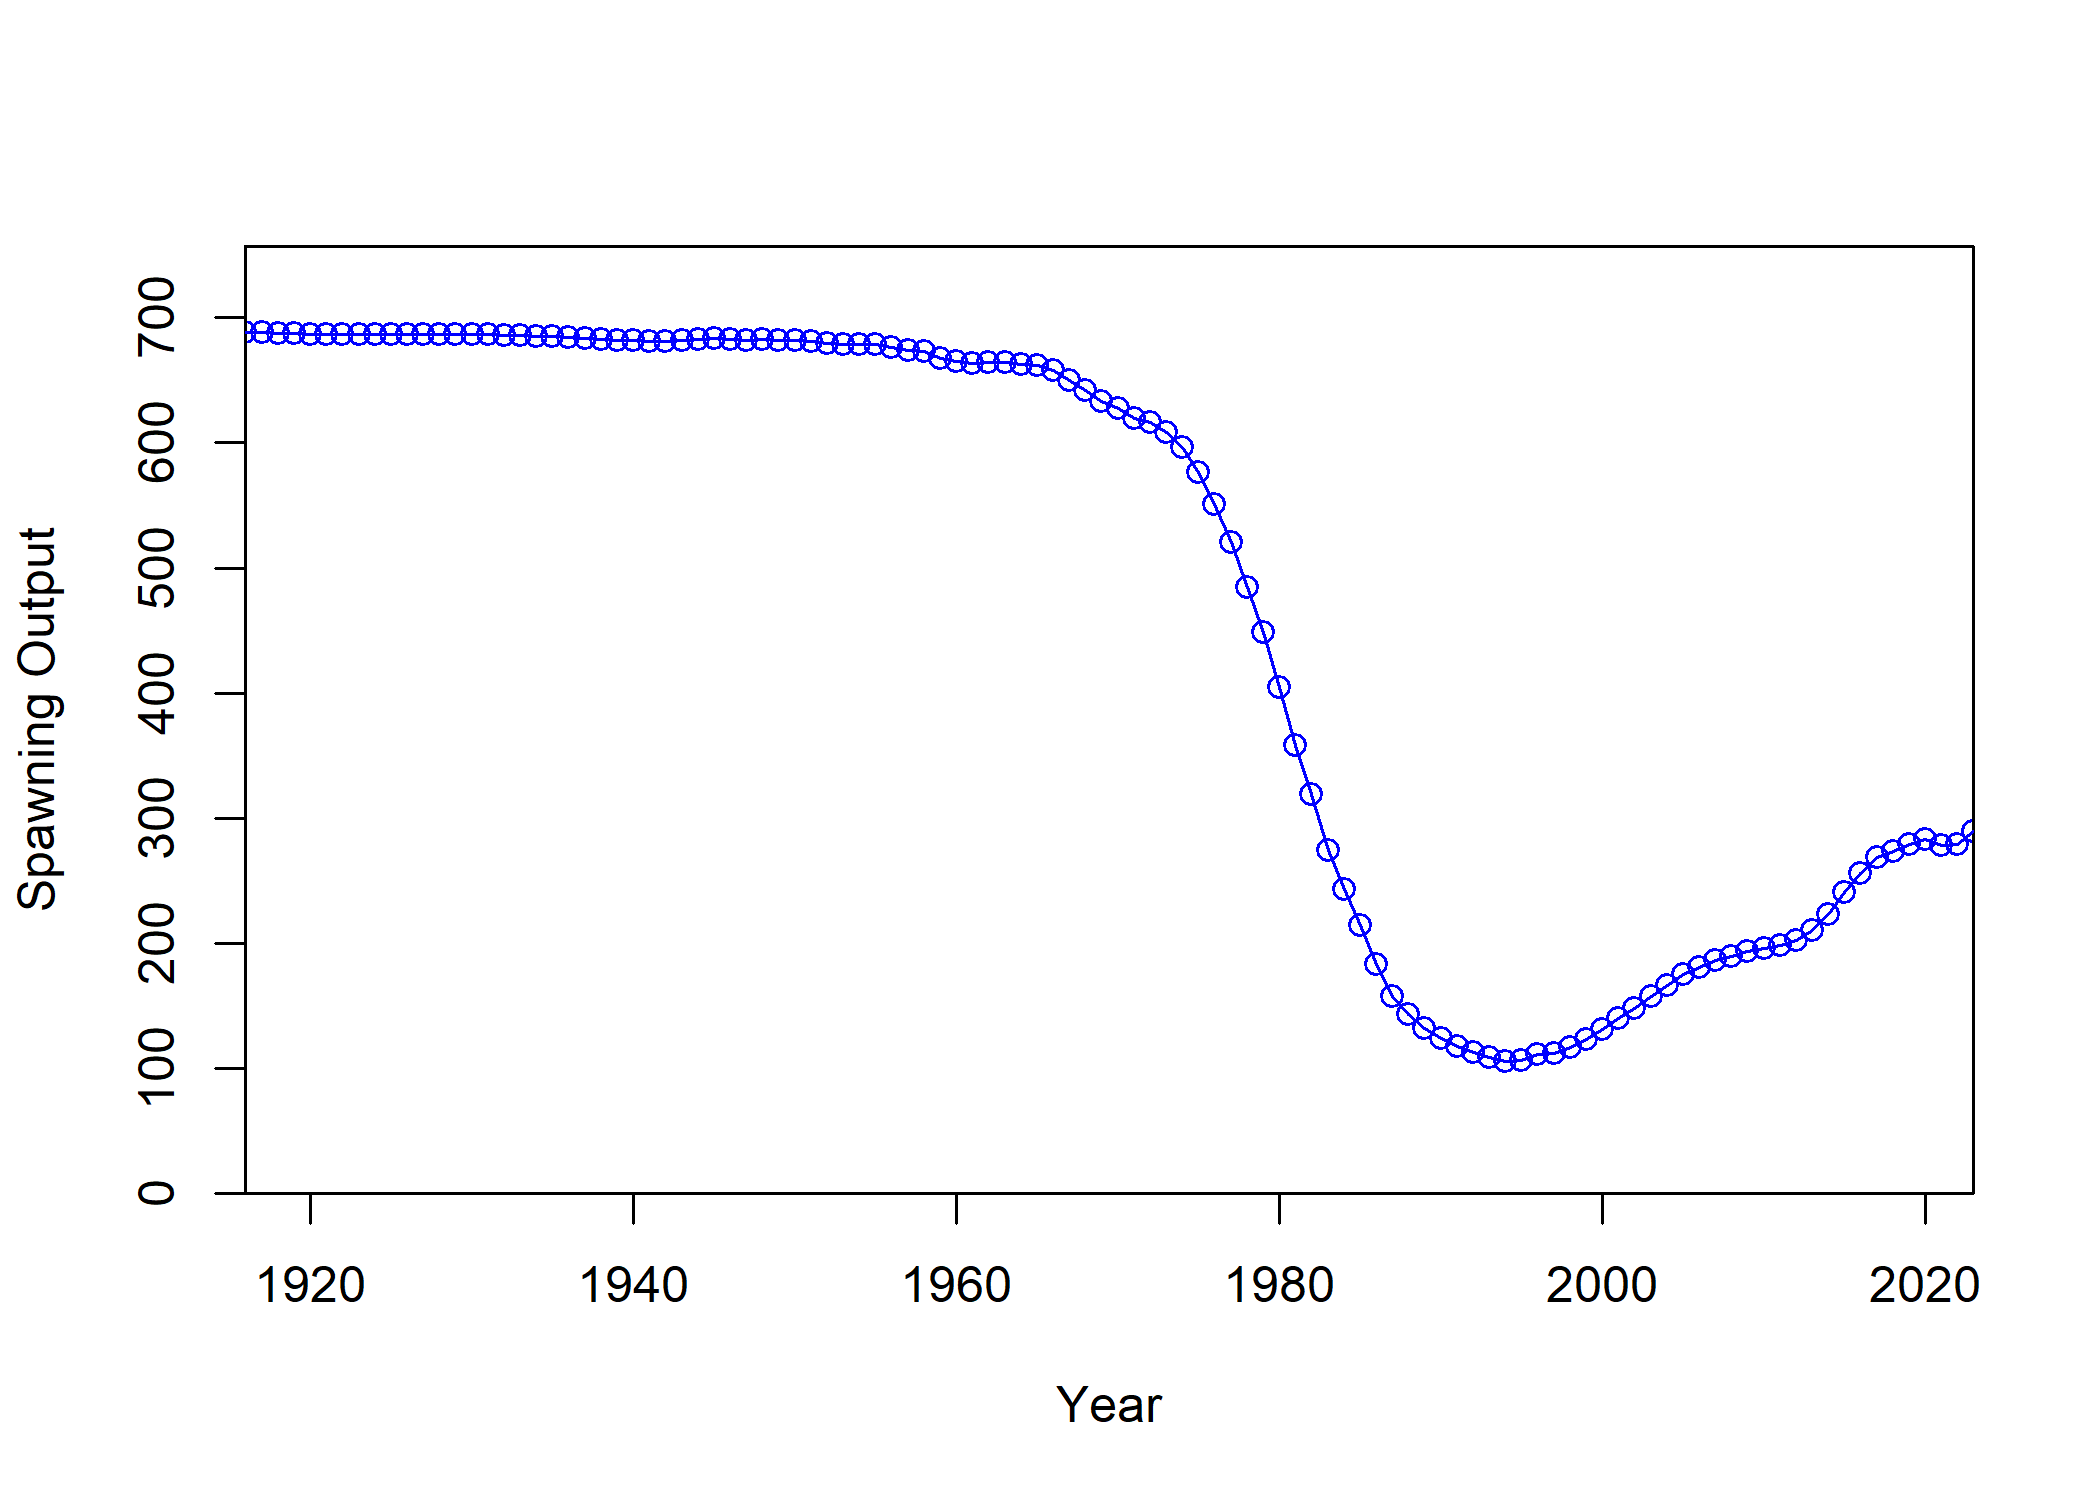
\includegraphics[width=1\textwidth,height=1\textheight]{C:/Assessments/2023/copper_rockfish_2023/documents/shared_figures/spawning_output_combined.png}
\caption{Estimated combined time series of spawning output for copper rockfish in California waters.\label{fig:es-sb-all}}
\end{figure}

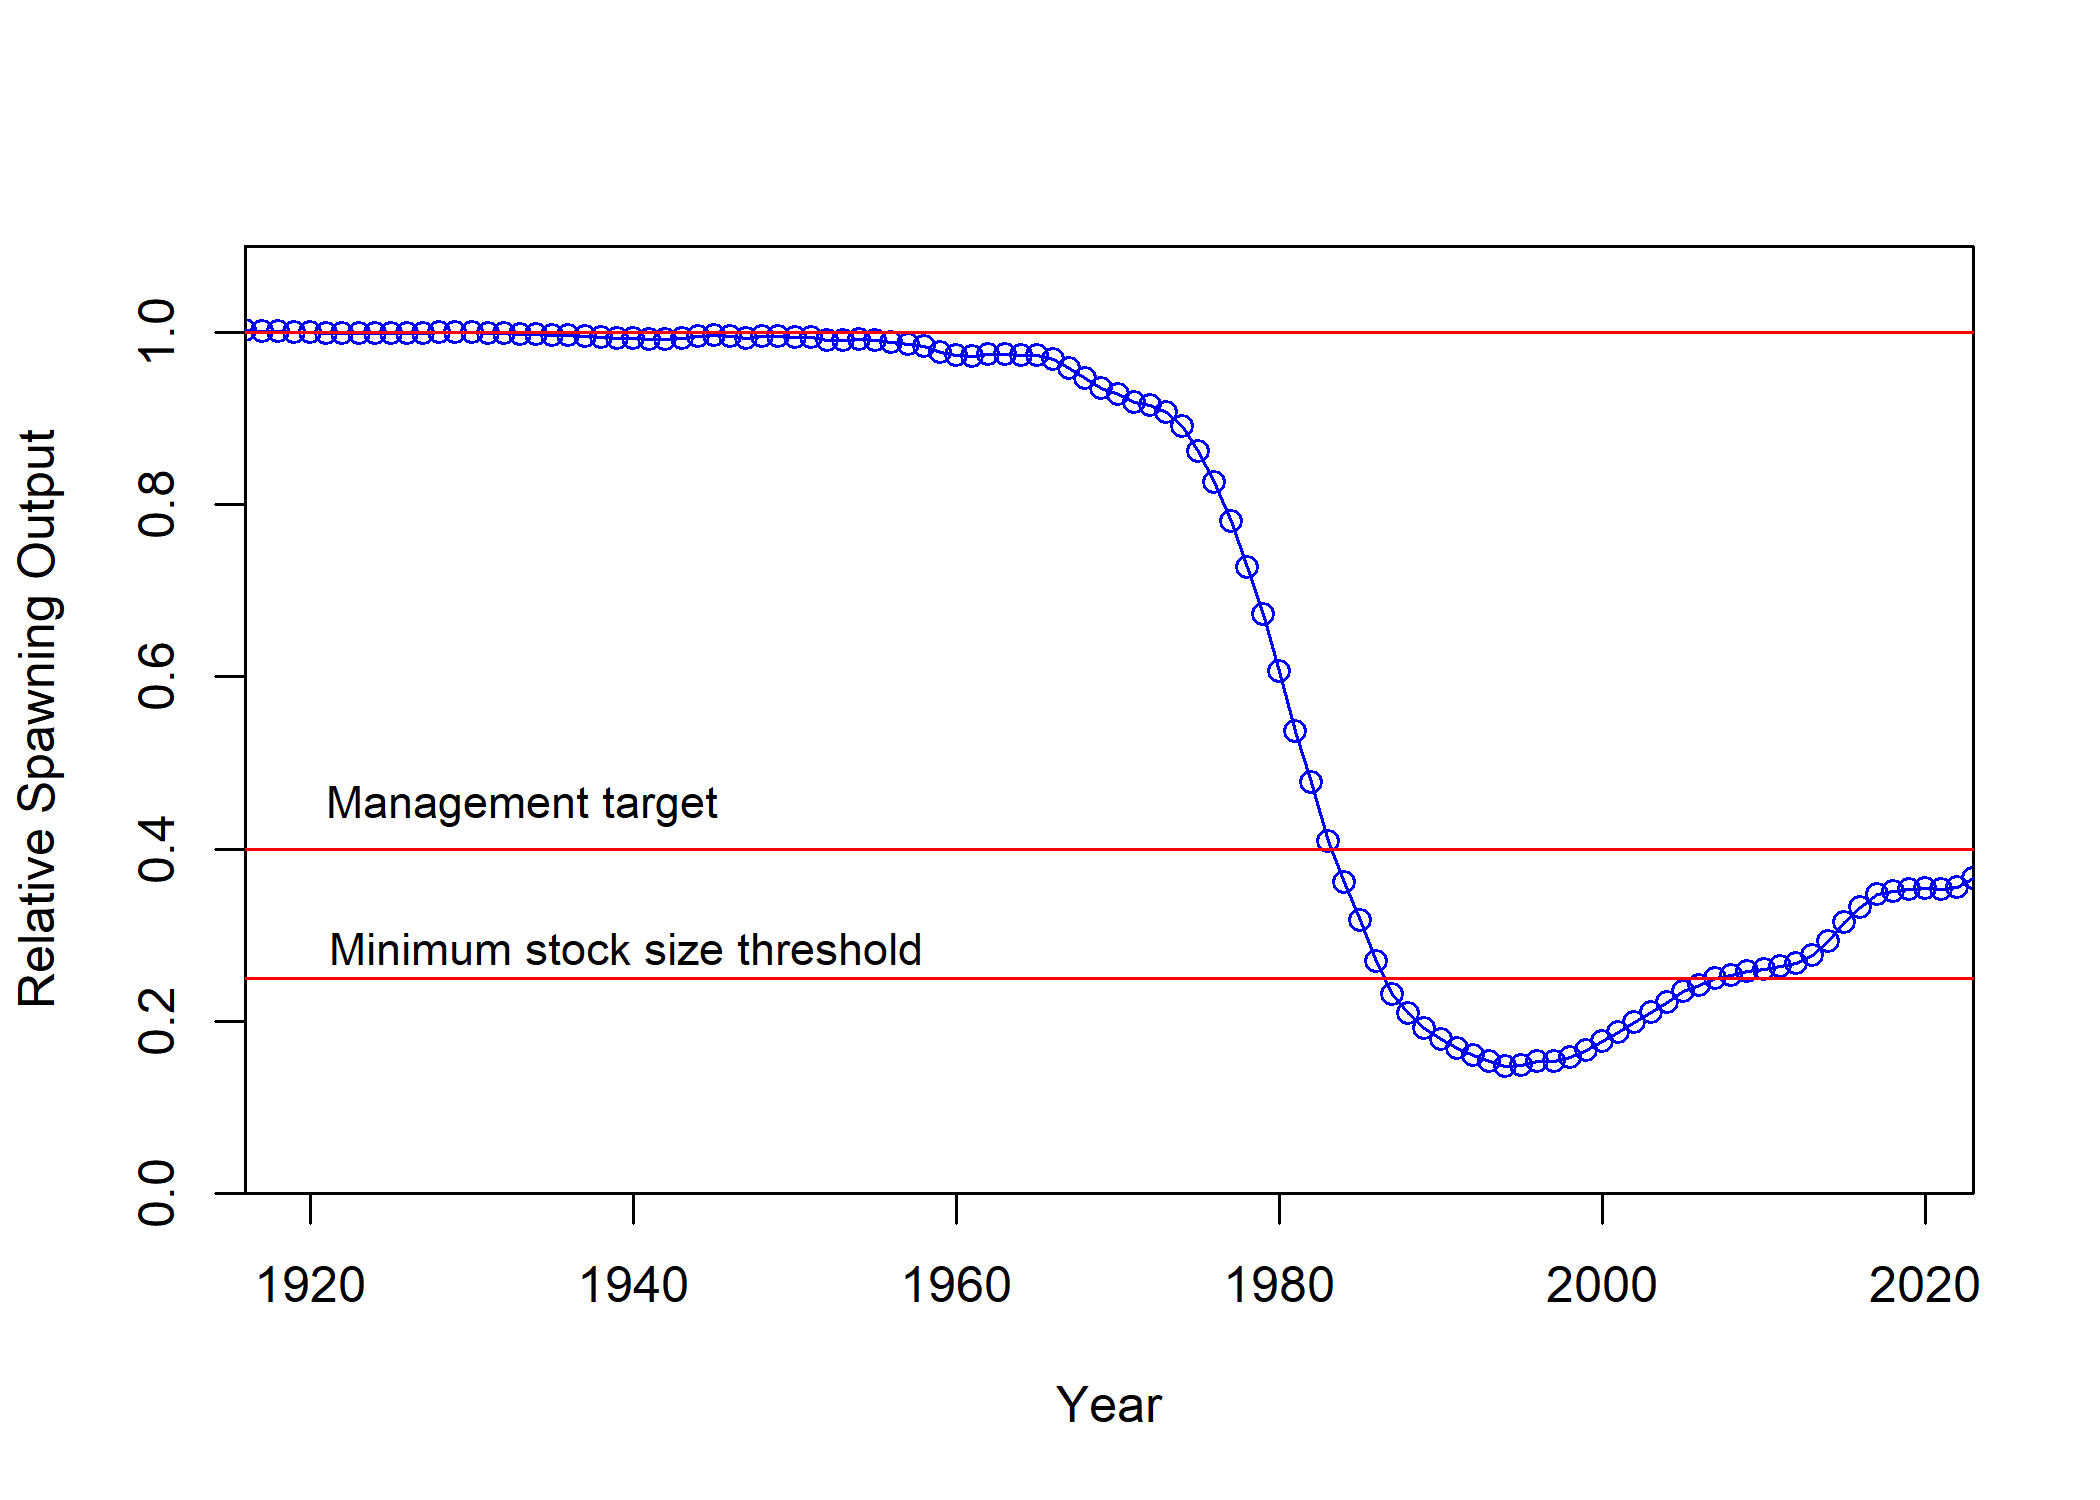
\includegraphics[width=1\textwidth,height=1\textheight]{C:/Assessments/2023/copper_rockfish_2023/documents/shared_figures/depletion_combined.png} \clearpage

\hypertarget{recruitment}{%
\subsection*{Recruitment}\label{recruitment}}
\addcontentsline{toc}{subsection}{Recruitment}

Replace text with trends and current levels relative to virgin or historic levels and description of uncertainty. Include Table for last 10 years. Include Figure with long-term estimates.

\begingroup\fontsize{10}{12}\selectfont
\begingroup\fontsize{10}{12}\selectfont

\begin{longtable}[t]{r>{\centering\arraybackslash}p{1.57cm}>{\centering\arraybackslash}p{1.57cm}>{\centering\arraybackslash}p{1.57cm}>{\centering\arraybackslash}p{1.57cm}>{\centering\arraybackslash}p{1.57cm}>{\centering\arraybackslash}p{1.57cm}}
\caption{\label{tab:south-recrES}Estimated recent trend in recruitment and recruitment deviations and the 95 percent intervals for the sub-area model south of Point Conception.}\\
\toprule
Year & Recruitment & Lower Interval & Upper Interval & Recruitment Deviations & Lower Interval & Upper Interval\\
\midrule
\endfirsthead
\caption[]{Estimated recent trend in recruitment and recruitment deviations and the 95 percent intervals for the sub-area model south of Point Conception. \textit{(continued)}}\\
\toprule
Year & Recruitment & Lower Interval & Upper Interval & Recruitment Deviations & Lower Interval & Upper Interval\\
\midrule
\endhead

\endfoot
\bottomrule
\endlastfoot
2013 & 613.62 & 381.00 & 988.26 & 1.18 & 0.94 & 1.41\\
2014 & 168.22 & 86.76 & 326.18 & -0.13 & -0.64 & 0.39\\
2015 & 81.26 & 39.81 & 165.88 & -0.88 & -1.45 & -0.30\\
2016 & 114.55 & 59.49 & 220.57 & -0.55 & -1.00 & -0.09\\
2017 & 91.14 & 44.28 & 187.61 & -0.79 & -1.33 & -0.25\\
2018 & 91.39 & 42.11 & 198.33 & -0.80 & -1.40 & -0.19\\
2019 & 119.56 & 51.10 & 279.76 & -0.53 & -1.24 & 0.18\\
2020 & 119.75 & 43.77 & 327.64 & -0.60 & -1.54 & 0.34\\
2021 & 231.44 & 144.36 & 371.04 & 0.00 & 0.00 & 0.00\\
2022 & 227.42 & 138.88 & 372.42 & 0.00 & 0.00 & 0.00\\
2023 & 226.18 & 137.68 & 371.57 & 0.00 & 0.00 & 0.00\\*
\end{longtable}
\endgroup{}
\endgroup{}


\begingroup\fontsize{10}{12}\selectfont
\begingroup\fontsize{10}{12}\selectfont

\begin{longtable}[t]{r>{\centering\arraybackslash}p{1.57cm}>{\centering\arraybackslash}p{1.57cm}>{\centering\arraybackslash}p{1.57cm}>{\centering\arraybackslash}p{1.57cm}>{\centering\arraybackslash}p{1.57cm}>{\centering\arraybackslash}p{1.57cm}}
\caption{\label{tab:north-recrES}Estimated recent trend in recruitment and recruitment deviations and the 95 percent intervals for the sub-area model north of Point Conception.}\\
\toprule
Year & Recruitment & Lower Interval & Upper Interval & Recruitment Deviations & Lower Interval & Upper Interval\\
\midrule
\endfirsthead
\caption[]{Estimated recent trend in recruitment and recruitment deviations and the 95 percent intervals for the sub-area model north of Point Conception. \textit{(continued)}}\\
\toprule
Year & Recruitment & Lower Interval & Upper Interval & Recruitment Deviations & Lower Interval & Upper Interval\\
\midrule
\endhead

\endfoot
\bottomrule
\endlastfoot
2013 & 556.60 & 282.67 & 1095.99 & 0.23 & -0.38 & 0.84\\
2014 & 466.50 & 233.22 & 933.12 & 0.04 & -0.59 & 0.67\\
2015 & 590.78 & 316.19 & 1103.84 & 0.26 & -0.27 & 0.79\\
2016 & 285.96 & 134.46 & 608.15 & -0.47 & -1.18 & 0.24\\
2017 & 869.76 & 474.53 & 1594.18 & 0.63 & 0.13 & 1.12\\
2018 & 618.32 & 318.82 & 1199.18 & 0.25 & -0.34 & 0.84\\
2019 & 345.34 & 159.74 & 746.57 & -0.37 & -1.11 & 0.37\\
2020 & 502.19 & 394.01 & 640.08 & 0.00 & 0.00 & 0.00\\
2021 & 503.74 & 394.44 & 643.32 & 0.00 & 0.00 & 0.00\\
2022 & 505.86 & 395.70 & 646.68 & 0.00 & 0.00 & 0.00\\
2023 & 509.39 & 398.85 & 650.56 & 0.00 & 0.00 & 0.00\\*
\end{longtable}
\endgroup{}
\endgroup{}


\begin{figure}
\centering
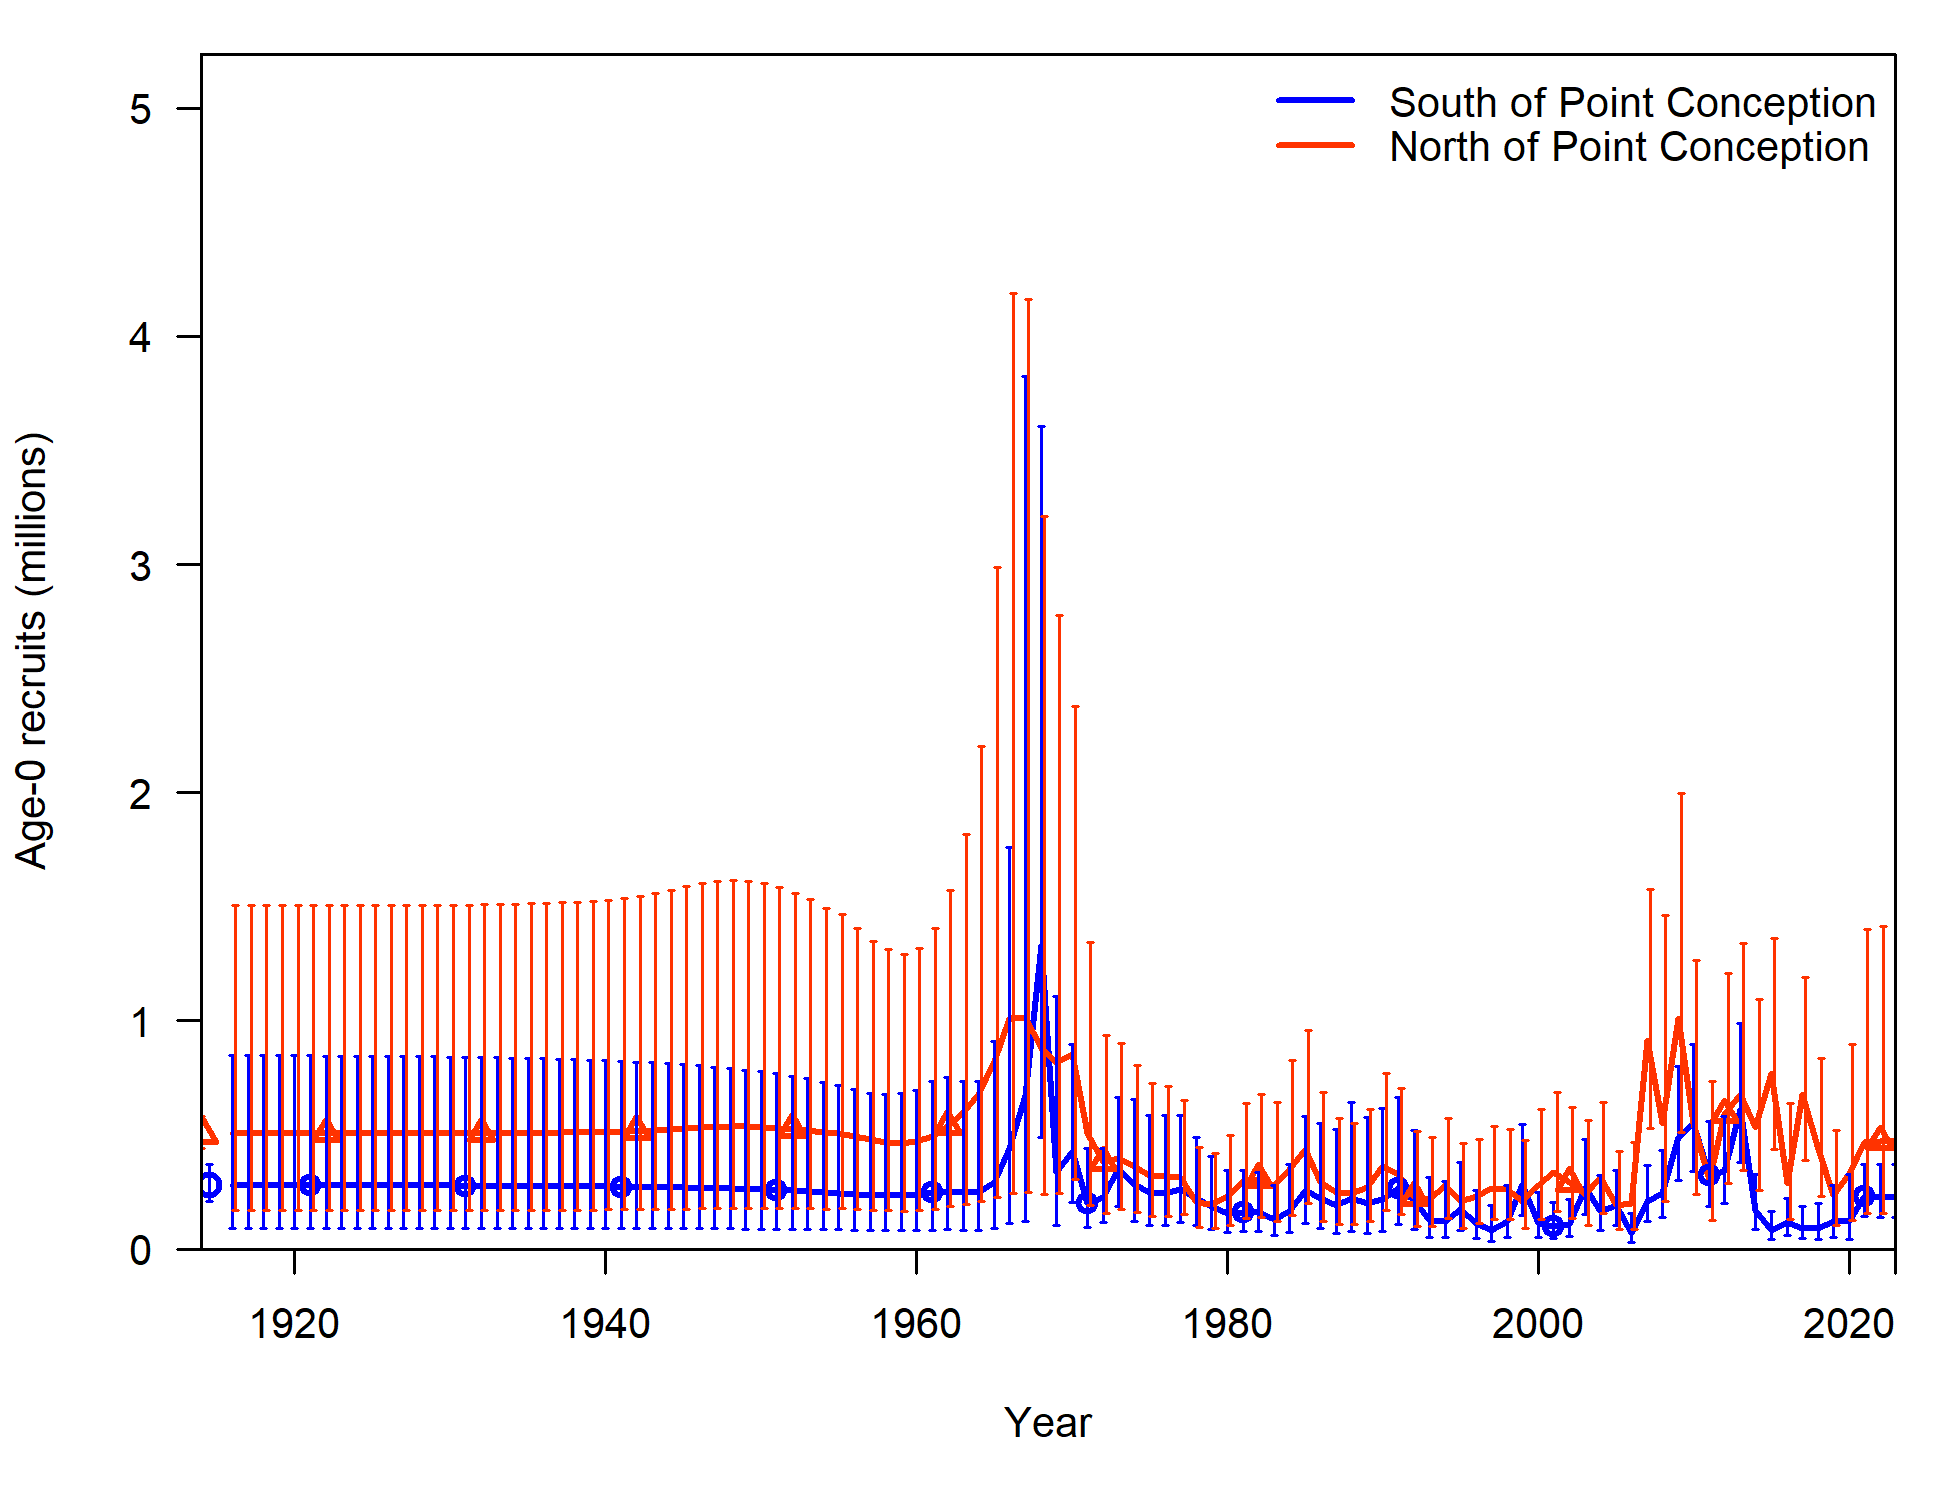
\includegraphics[width=1\textwidth,height=1\textheight]{C:/Assessments/2023/copper_rockfish_2023/documents/shared_figures/compare10_recruits_uncertainty.png}
\caption{Estimated time series of age-0 recruits (1000s) for the model areas south and north of Point Conception with 95 percent intervals.\label{fig:es-recruits}}
\end{figure}

\begin{figure}
\centering
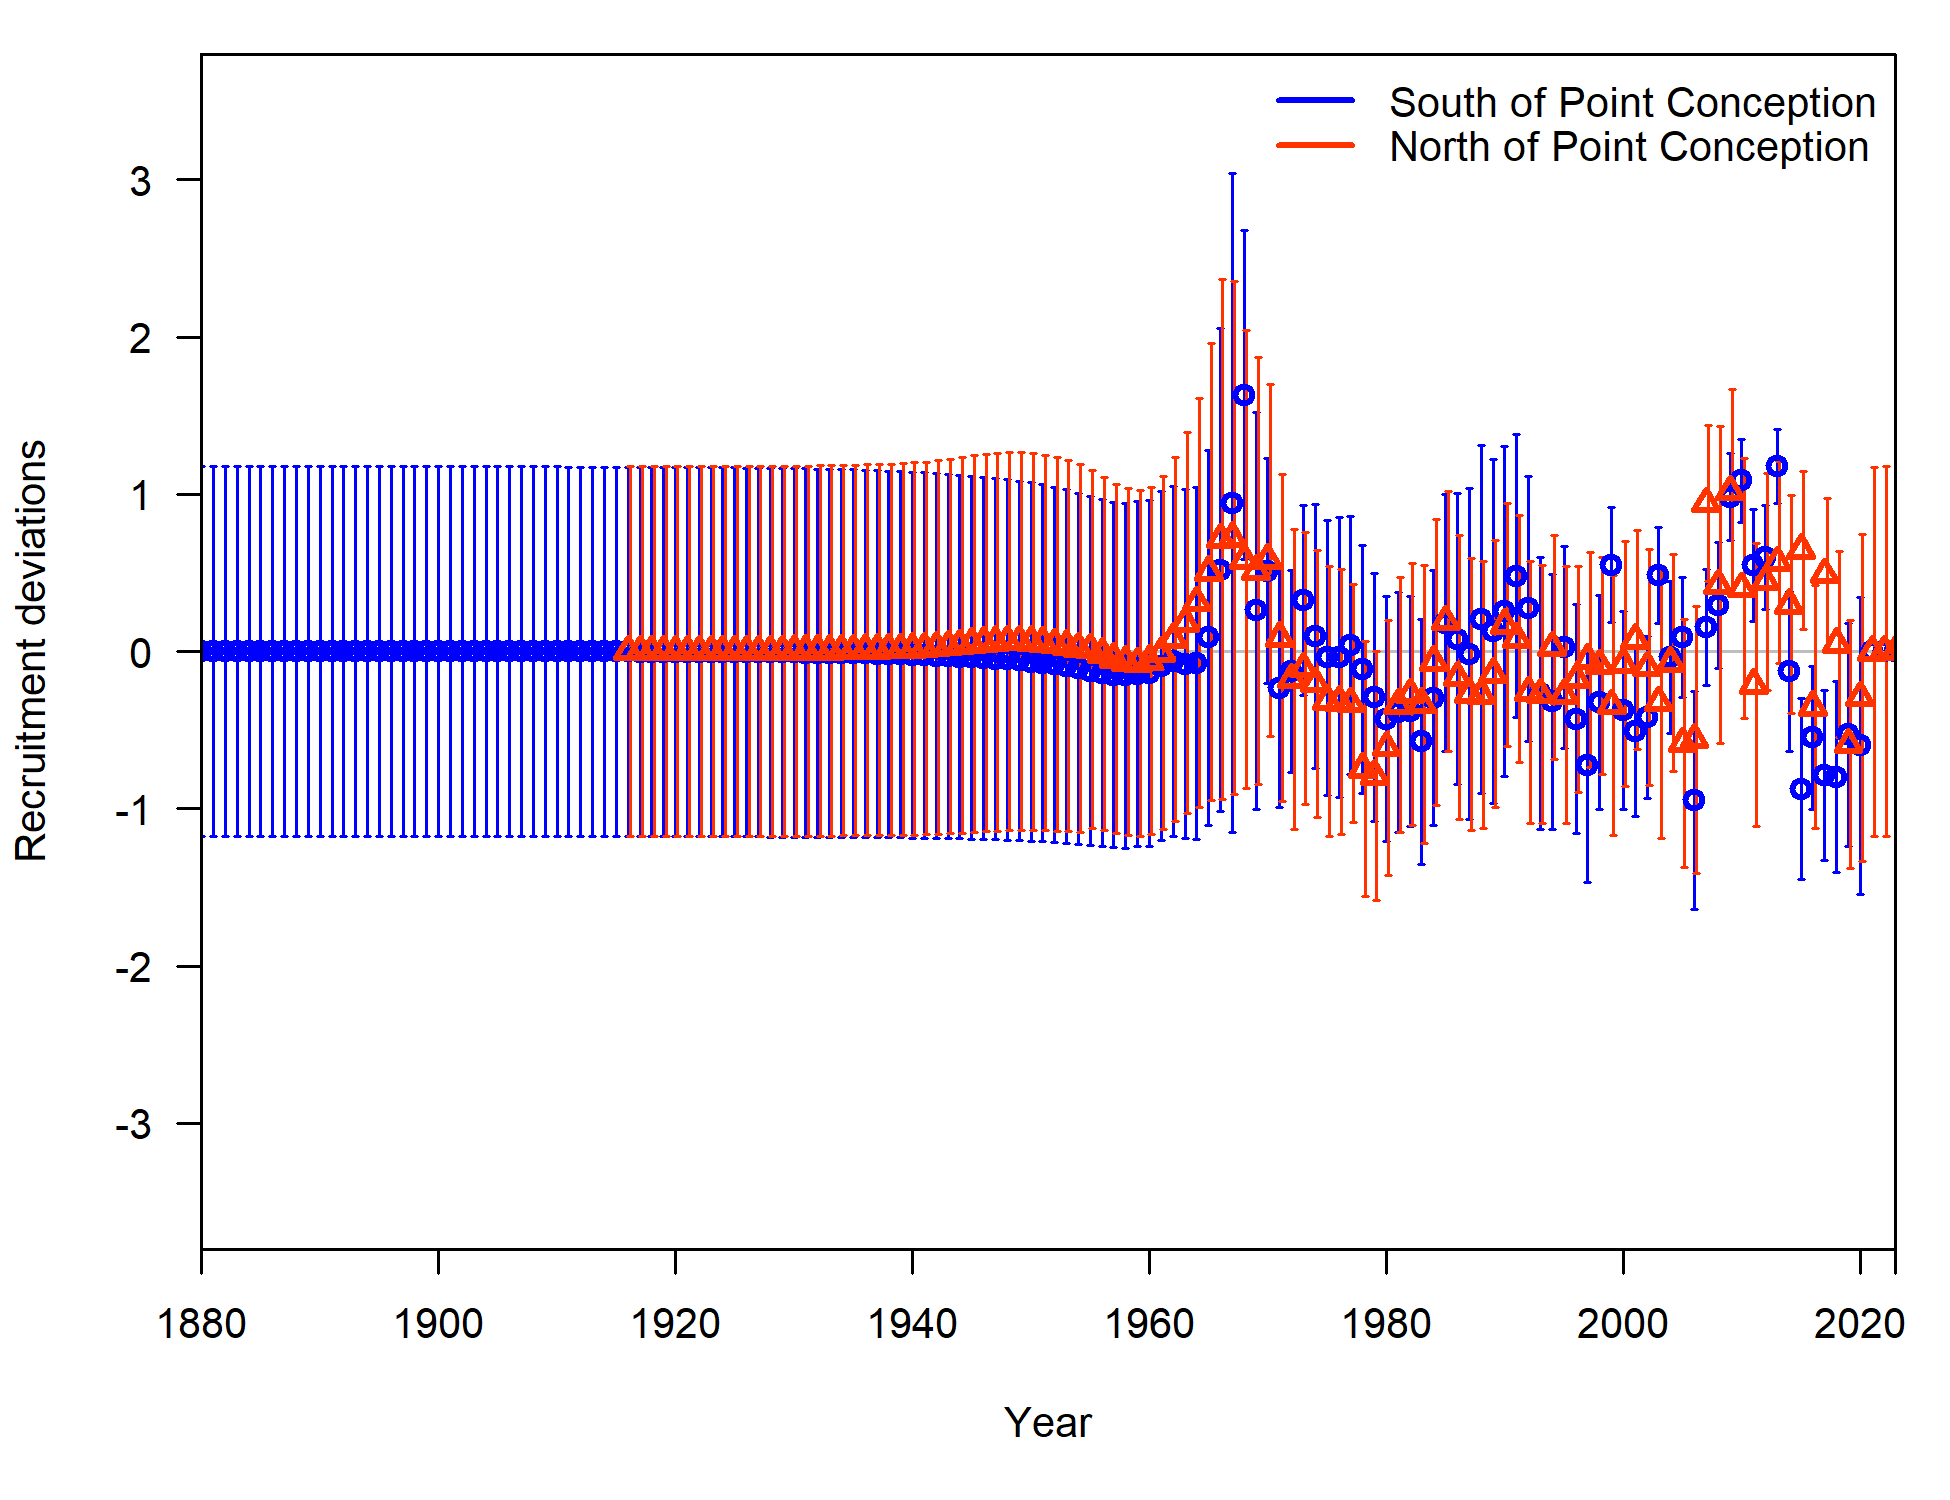
\includegraphics[width=1\textwidth,height=1\textheight]{C:/Assessments/2023/copper_rockfish_2023/documents/shared_figures/compare12_recdevs_uncertainty.png}
\caption{Estimated time series of recruitment deviations for the model areas south and north of Point Conception.\label{fig:es-rec-devs}}
\end{figure}

\clearpage

\hypertarget{exploitation-status}{%
\subsection*{Exploitation status}\label{exploitation-status}}
\addcontentsline{toc}{subsection}{Exploitation status}

Replace text with total catch divided by exploitable biomass or SPR harvest rate. Include Table for last 10 years. Include Figure with trend in f relative to target vs.~trend in biomass relative to the target.

\begingroup\fontsize{10}{12}\selectfont
\begingroup\fontsize{10}{12}\selectfont

\begin{longtable}[t]{r>{\centering\arraybackslash}p{1.57cm}>{\centering\arraybackslash}p{1.57cm}>{\centering\arraybackslash}p{1.57cm}>{\centering\arraybackslash}p{1.57cm}>{\centering\arraybackslash}p{1.57cm}>{\centering\arraybackslash}p{1.57cm}}
\caption{\label{tab:south-exploitES}Estimated recent trend in the 1-SPR where SPR is the spawning potential ratio the exploitation rate, and the 95 percent intervals for the sub-area model south of Point Conception.}\\
\toprule
Year & 1-SPR & Lower Interval & Upper Interval & Exploitation Rate & Lower Interval & Upper Interval\\
\midrule
\endfirsthead
\caption[]{Estimated recent trend in the 1-SPR where SPR is the spawning potential ratio the exploitation rate, and the 95 percent intervals for the sub-area model south of Point Conception. \textit{(continued)}}\\
\toprule
Year & 1-SPR & Lower Interval & Upper Interval & Exploitation Rate & Lower Interval & Upper Interval\\
\midrule
\endhead

\endfoot
\bottomrule
\endlastfoot
2013 & 0.71 & 0.52 & 0.90 & 0.11 & 0.05 & 0.17\\
2014 & 0.59 & 0.39 & 0.79 & 0.08 & 0.04 & 0.13\\
2015 & 0.66 & 0.46 & 0.86 & 0.10 & 0.05 & 0.16\\
2016 & 0.71 & 0.51 & 0.90 & 0.12 & 0.05 & 0.18\\
2017 & 0.67 & 0.46 & 0.88 & 0.10 & 0.04 & 0.16\\
2018 & 0.75 & 0.55 & 0.95 & 0.12 & 0.05 & 0.20\\
2019 & 0.72 & 0.50 & 0.94 & 0.11 & 0.03 & 0.18\\
2020 & 0.80 & 0.59 & 1.01 & 0.12 & 0.03 & 0.21\\
2021 & 0.72 & 0.47 & 0.98 & 0.09 & 0.02 & 0.17\\
2022 & 0.40 & 0.15 & 0.64 & 0.03 & 0.01 & 0.06\\*
\end{longtable}
\endgroup{}
\endgroup{}


\begingroup\fontsize{10}{12}\selectfont
\begingroup\fontsize{10}{12}\selectfont

\begin{longtable}[t]{r>{\centering\arraybackslash}p{1.57cm}>{\centering\arraybackslash}p{1.57cm}>{\centering\arraybackslash}p{1.57cm}>{\centering\arraybackslash}p{1.57cm}>{\centering\arraybackslash}p{1.57cm}>{\centering\arraybackslash}p{1.57cm}}
\caption{\label{tab:north-exploitES}Estimated recent trend in the 1-SPR where SPR is the spawning potential ratio the exploitation rate, and the 95 percent intervals for the sub-area model north of Point Conception.}\\
\toprule
Year & 1-SPR & Lower Interval & Upper Interval & Exploitation Rate & Lower Interval & Upper Interval\\
\midrule
\endfirsthead
\caption[]{Estimated recent trend in the 1-SPR where SPR is the spawning potential ratio the exploitation rate, and the 95 percent intervals for the sub-area model north of Point Conception. \textit{(continued)}}\\
\toprule
Year & 1-SPR & Lower Interval & Upper Interval & Exploitation Rate & Lower Interval & Upper Interval\\
\midrule
\endhead

\endfoot
\bottomrule
\endlastfoot
2013 & 0.16 & 0.10 & 0.22 & 0.01 & 0.01 & 0.02\\
2014 & 0.20 & 0.13 & 0.27 & 0.02 & 0.01 & 0.02\\
2015 & 0.31 & 0.21 & 0.41 & 0.03 & 0.02 & 0.04\\
2016 & 0.31 & 0.20 & 0.41 & 0.03 & 0.02 & 0.04\\
2017 & 0.50 & 0.37 & 0.63 & 0.05 & 0.03 & 0.08\\
2018 & 0.41 & 0.28 & 0.53 & 0.04 & 0.02 & 0.06\\
2019 & 0.40 & 0.27 & 0.53 & 0.04 & 0.02 & 0.06\\
2020 & 0.53 & 0.38 & 0.67 & 0.06 & 0.03 & 0.08\\
2021 & 0.41 & 0.27 & 0.55 & 0.04 & 0.02 & 0.06\\
2022 & 0.21 & 0.12 & 0.30 & 0.02 & 0.01 & 0.03\\*
\end{longtable}
\endgroup{}
\endgroup{}


\begin{figure}
\centering
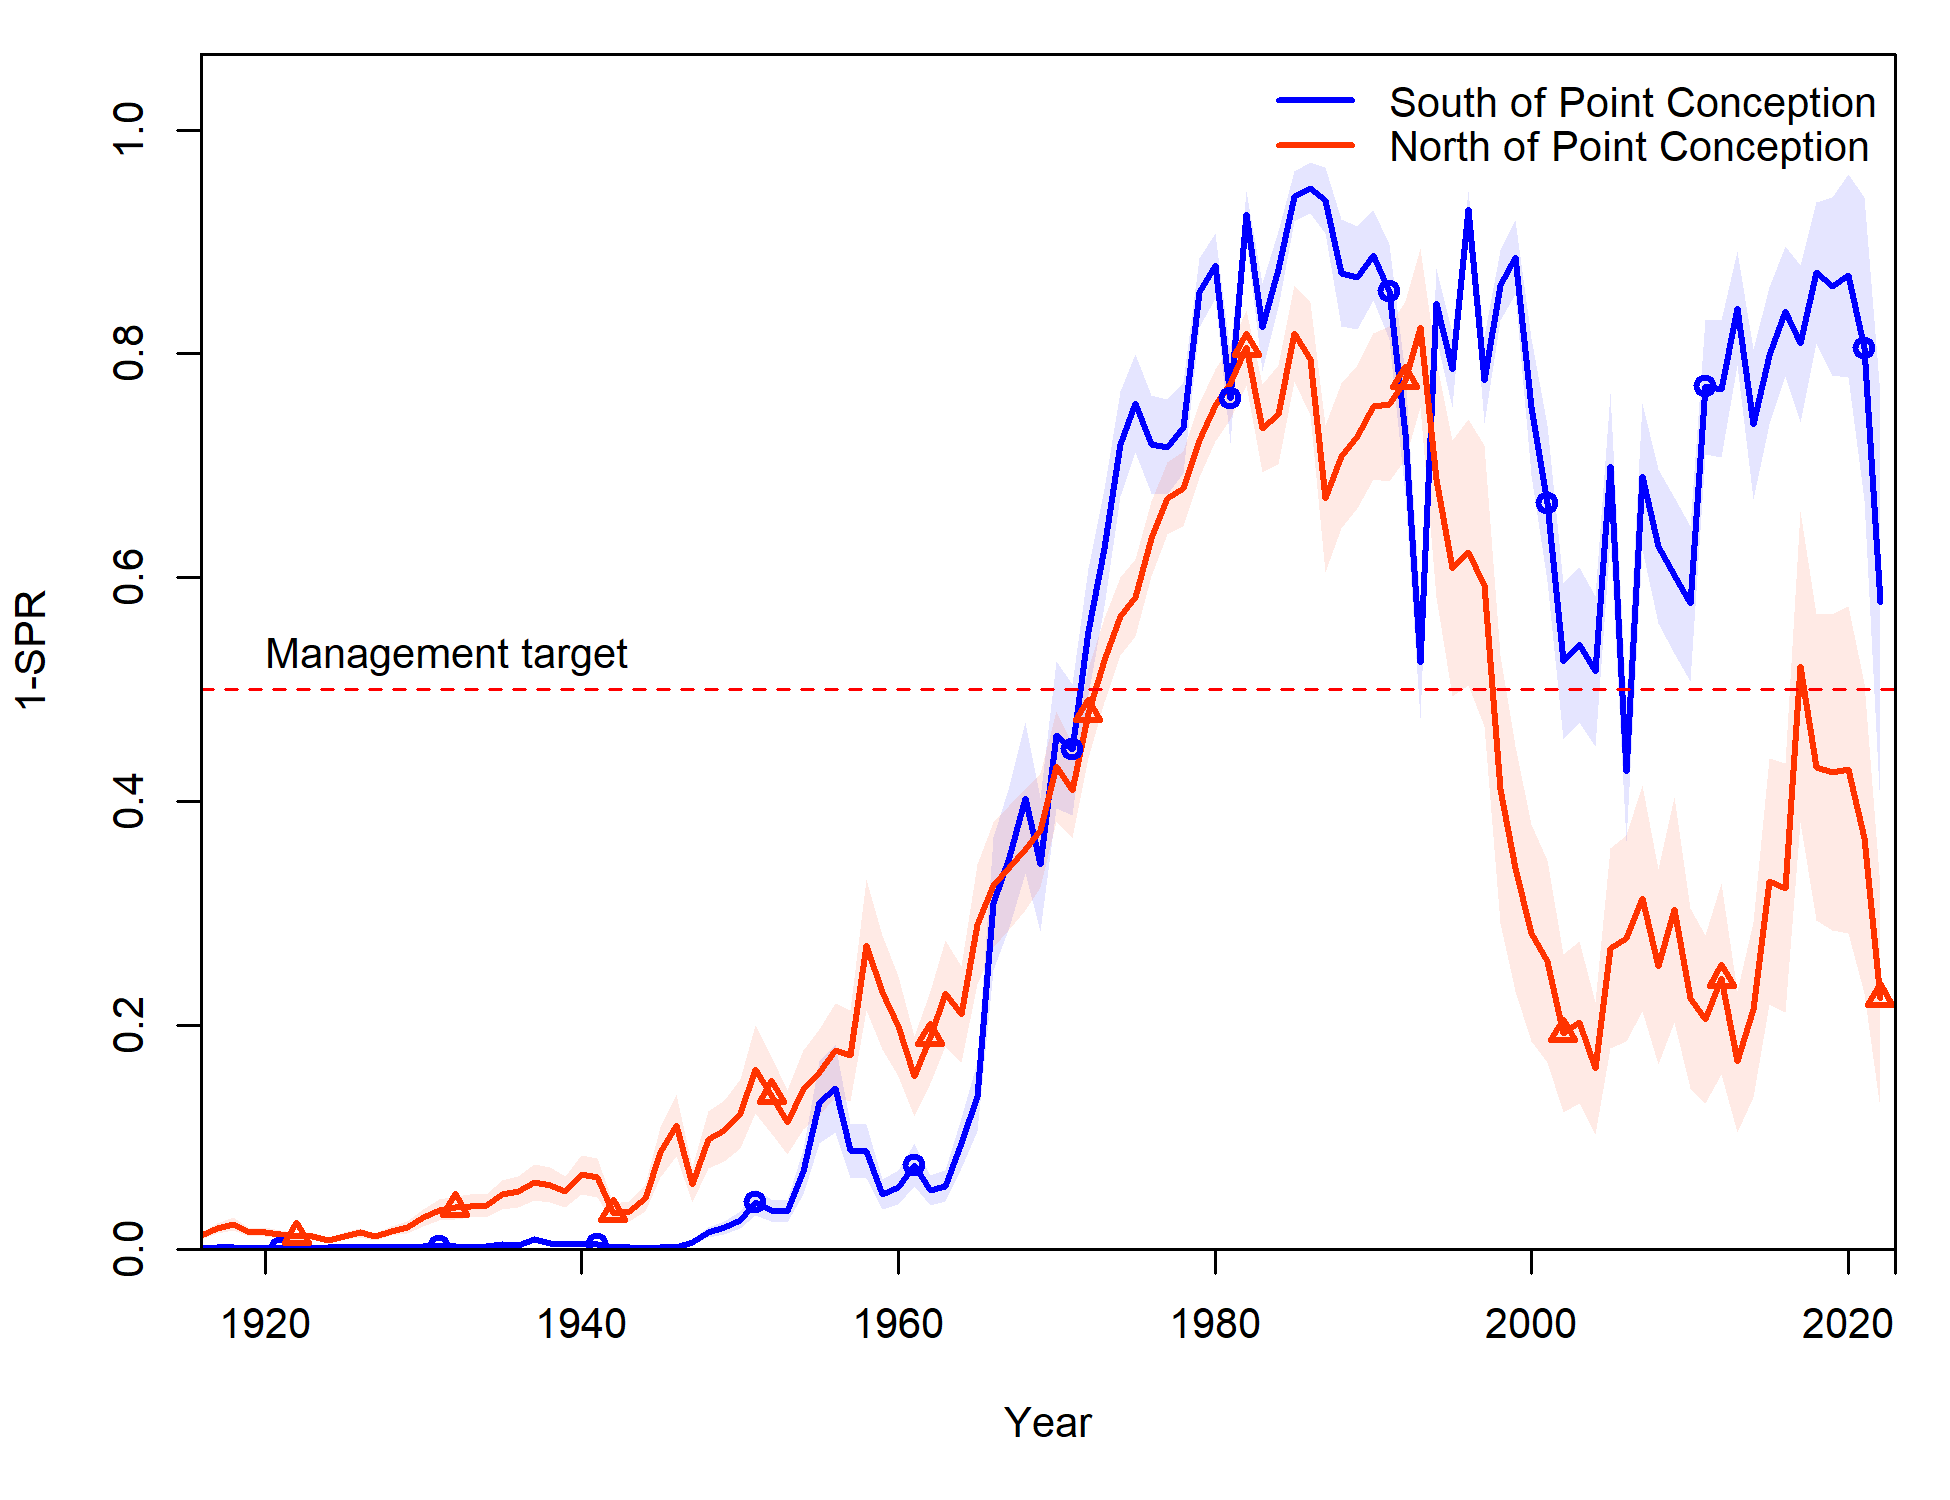
\includegraphics[width=1\textwidth,height=1\textheight]{C:/Assessments/2023/copper_rockfish_2023/documents/shared_figures/compare6_SPRratio_uncertainty.png}
\caption{Estimated 1 - relative spawning ratio (SPR) by year for the model areas south and north of Point Conception. The management target is plotted as a red horizontal line and values above this reflect harvest in excess of the proxy harvest rate.\label{fig:es-1-spr}}
\end{figure}

\hypertarget{ecosystem-considerations}{%
\subsection*{Ecosystem considerations}\label{ecosystem-considerations}}
\addcontentsline{toc}{subsection}{Ecosystem considerations}

shared text

\hypertarget{reference-points}\), i.e., the \(B_{MSY}\) proxy and the equilibrium stock size that results from fishing at the default harvest rate, i.e., the \(F_{MSY}\) proxy. Include Table of estimated reference points for ssb, SPR, exploitation rate, and yield based on SSB proxy for MSY, SPR proxy for MSY, and estimated MSY values.

\begingroup\fontsize{10}{12}\selectfont
\begingroup\fontsize{10}{12}\selectfont

\begin{longtable}[t]{r>{\centering\arraybackslash}p{2cm}>{\centering\arraybackslash}p{2cm}>{\centering\arraybackslash}p{2cm}}
\caption{\label{tab:south-referenceES}Summary of reference points and management quantities, including estimates of the 95 percent intervals for the sub-area model south of Point Conception.}\\
\toprule
 & Estimate & Lower Interval & Upper Interval\\
\midrule
\endfirsthead
\caption[]{Summary of reference points and management quantities, including estimates of the 95 percent intervals for the sub-area model south of Point Conception. \textit{(continued)}}\\
\toprule
 & Estimate & Lower Interval & Upper Interval\\
\midrule
\endhead

\endfoot
\bottomrule
\endlastfoot
Unfished Spawning Output & 201.06 & 163.43 & 238.70\\
Unfished Age 3+ Biomass (mt) & 1999.51 & 1624.90 & 2374.12\\
Unfished Recruitment (R0) & 241.18 & 196.04 & 286.32\\
Spawning Output (2023) & 32.06 & 12.70 & 51.42\\
Fraction Unfished (2023) & 0.16 & 0.06 & 0.25\\
Reference Points Based SB40\% &  &  & \\
Proxy Spawning Output SB40\% & 80.43 & 65.37 & 95.48\\
SPR Resulting in SB40\% & 0.46 & 0.46 & 0.46\\
Exploitation Rate Resulting in SB40\% & 0.06 & 0.05 & 0.06\\
Yield with SPR Based On SB40\% (mt) & 49.99 & 40.74 & 59.25\\
Reference Points Based on SPR Proxy for MSY &  &  & \\
Proxy Spawning Output (SPR50) & 89.71 & 72.92 & 106.50\\
SPR50 & 0.50 & - & -\\
Exploitation Rate Corresponding to SPR50 & 0.05 & 0.05 & 0.05\\
Yield with SPR50 at SB SPR (mt) & 47.78 & 38.93 & 56.62\\
Reference Points Based on Estimated MSY Values &  &  & \\
Spawning Output at MSY (SB MSY) & 55.51 & 45.15 & 65.87\\
SPR MSY & 0.35 & 0.34 & 0.35\\
Exploitation Rate Corresponding to SPR MSY & 0.08 & 0.08 & 0.08\\
MSY (mt) & 52.94 & 43.14 & 62.74\\*
\end{longtable}
\endgroup{}
\endgroup{}


\begingroup\fontsize{10}{12}\selectfont
\begingroup\fontsize{10}{12}\selectfont

\begin{longtable}[t]{r>{\centering\arraybackslash}p{2cm}>{\centering\arraybackslash}p{2cm}>{\centering\arraybackslash}p{2cm}}
\caption{\label{tab:north-referenceES}Summary of reference points and management quantities, including estimates of the 95 percent intervals for the sub-area model north of Point Conception.}\\
\toprule
 & Estimate & Lower Interval & Upper Interval\\
\midrule
\endfirsthead
\caption[]{Summary of reference points and management quantities, including estimates of the 95 percent intervals for the sub-area model north of Point Conception. \textit{(continued)}}\\
\toprule
 & Estimate & Lower Interval & Upper Interval\\
\midrule
\endhead

\endfoot
\bottomrule
\endlastfoot
Unfished Spawning Output & 486.15 & 387.43 & 584.87\\
Unfished Age 3+ Biomass (mt) & 4719.91 & 3777.92 & 5661.90\\
Unfished Recruitment (R0) & 567.77 & 452.48 & 683.06\\
Spawning Output (2023) & 262.10 & 124.28 & 399.92\\
Fraction Unfished (2023) & 0.54 & 0.32 & 0.76\\
Reference Points Based SB40\% &  &  & \\
Proxy Spawning Output SB40\% & 194.46 & 154.97 & 233.95\\
SPR Resulting in SB40\% & 0.46 & 0.46 & 0.46\\
Exploitation Rate Resulting in SB40\% & 0.06 & 0.06 & 0.06\\
Yield with SPR Based On SB40\% (mt) & 129.86 & 104.05 & 155.67\\
Reference Points Based on SPR Proxy for MSY &  &  & \\
Proxy Spawning Output (SPR50) & 216.90 & 172.85 & 260.94\\
SPR50 & 0.50 &  & \\
Exploitation Rate Corresponding to SPR50 & 0.05 & 0.05 & 0.05\\
Yield with SPR50 at SB SPR (mt) & 124.05 & 99.39 & 148.71\\
Reference Points Based on Estimated MSY Values &  &  & \\
Spawning Output at MSY (SB MSY) & 134.17 & 106.84 & 161.51\\
SPR MSY & 0.35 & 0.34 & 0.35\\
Exploitation Rate Corresponding to SPR MSY & 0.09 & 0.08 & 0.09\\
MSY (mt) & 137.59 & 110.25 & 164.92\\*
\end{longtable}
\endgroup{}
\endgroup{}


\begin{figure}
\centering
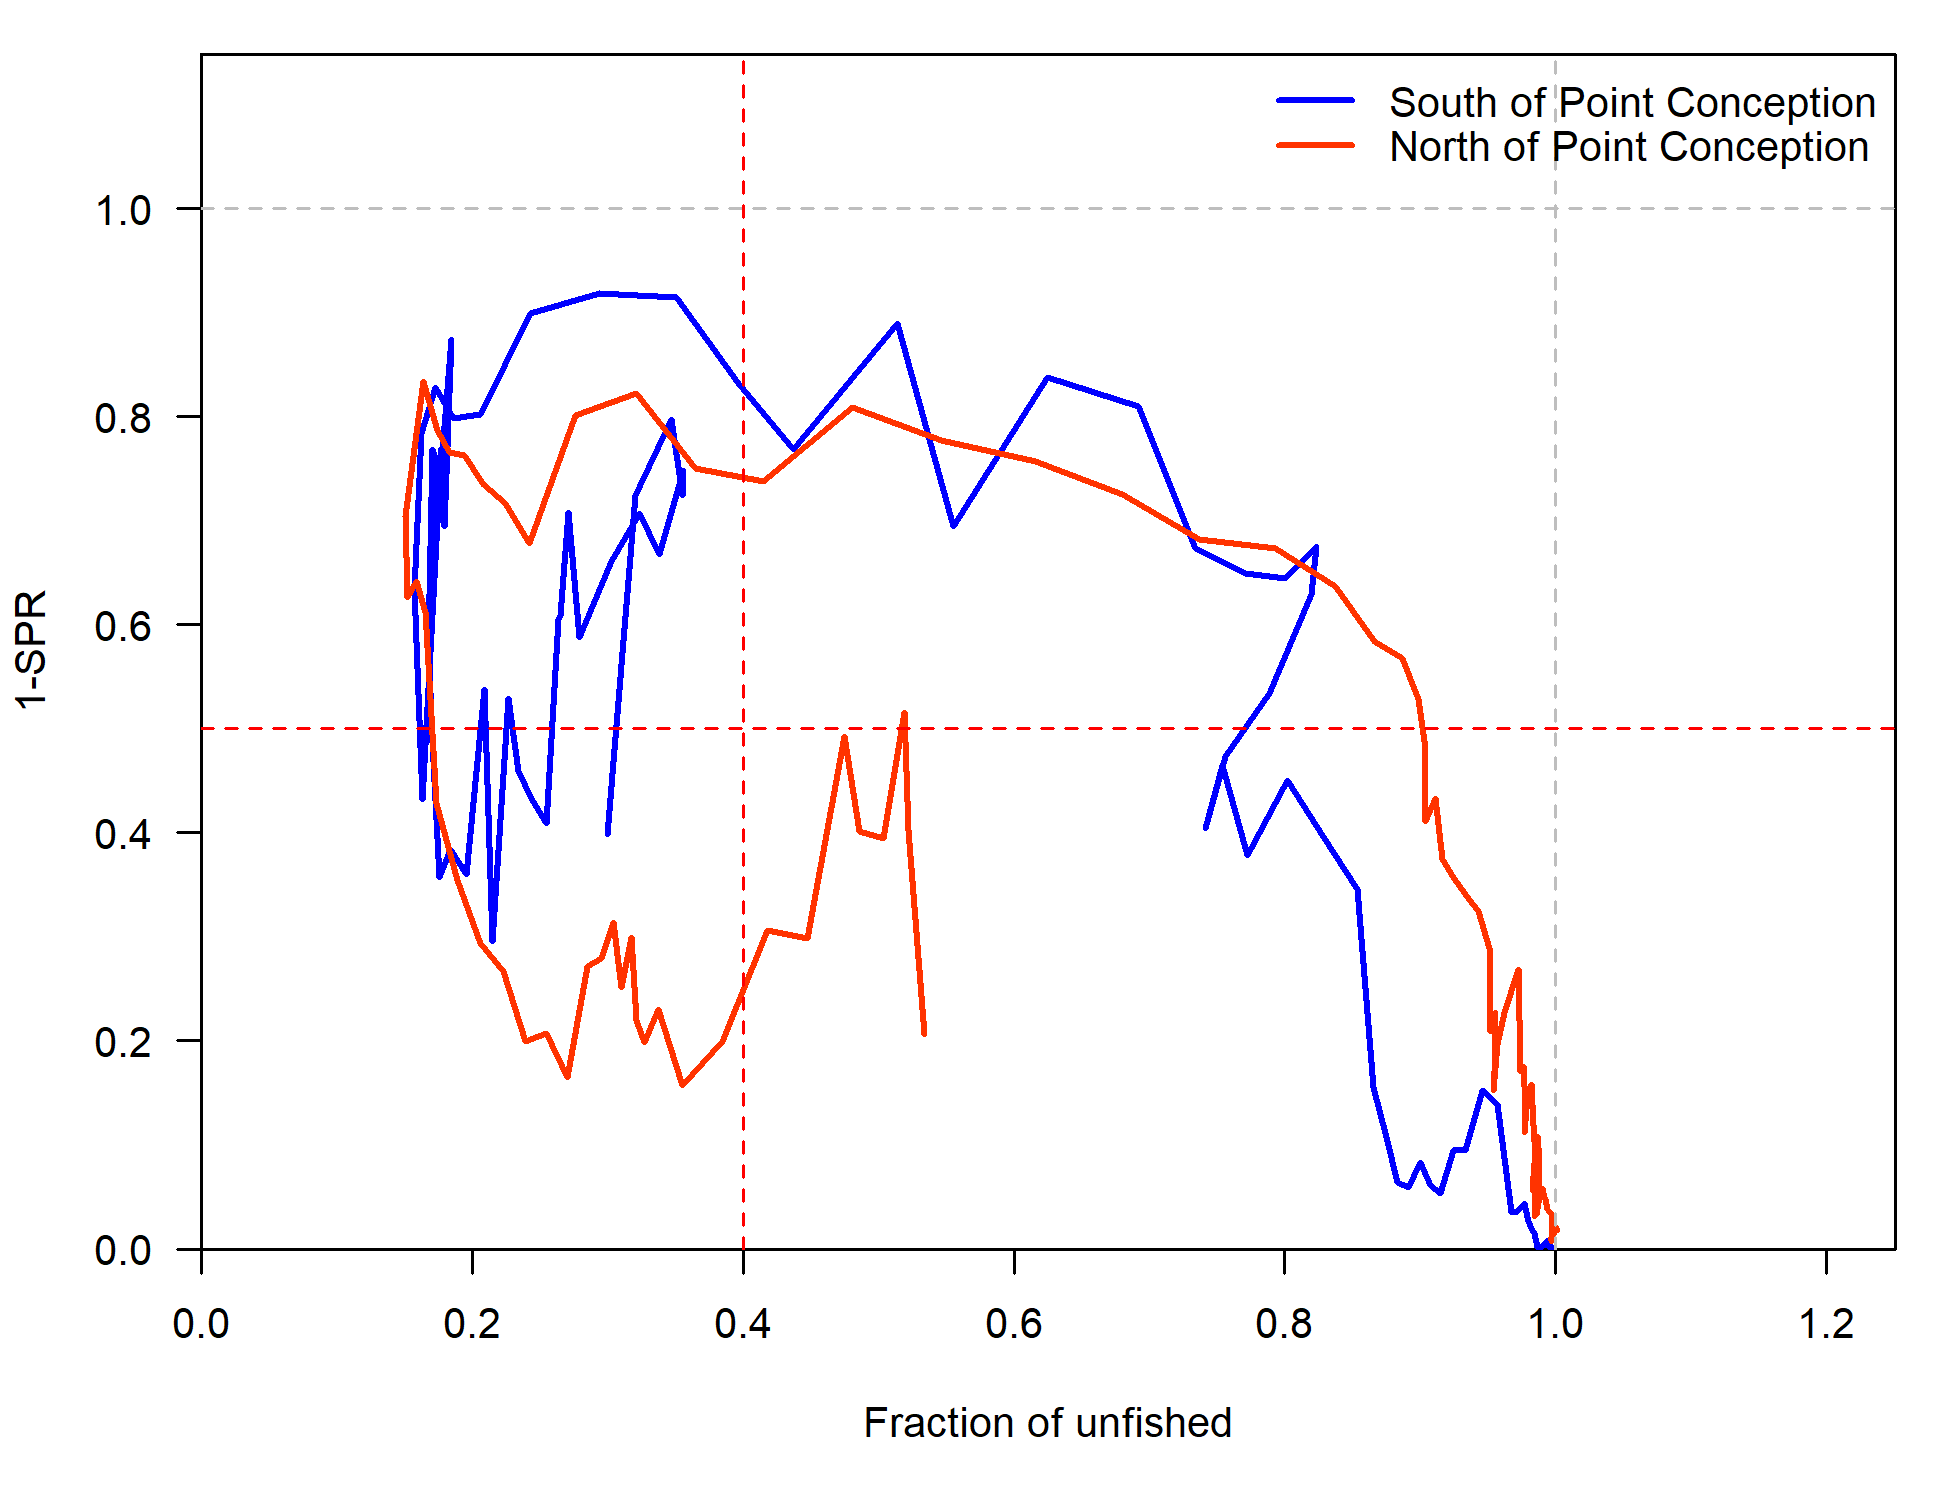
\includegraphics[width=1\textwidth,height=1\textheight]{C:/Assessments/2023/copper_rockfish_2023/documents/shared_figures/compare15_phase_plot.png}
\caption{Phase plot of estimated 1-SPR versus fraction unfished for the model areas south and north of Point Conception.\label{fig:es-phase}}
\end{figure}

\begin{figure}
\centering
\includegraphics[width=1\textwidth,height=1\textheight]{N:/Assessments/CurrentAssessments/copper_rockfish_2023/models/sca/14.0_base_forecast/plots/yield2_yield_curve_with_refpoints.png}
\caption{Equilibrium yield curve for the base case model for model south of Point Conception. Values are based on the 2022 fishery selectivities and with steepness fixed at 0.72.\label{fig:south-es-yield}}
\end{figure}

\begin{figure}
\centering
\includegraphics[width=1\textwidth,height=1\textheight]{N:/Assessments/CurrentAssessments/copper_rockfish_2023/models/nca/9.8_selex_fix_forecast/plots/yield2_yield_curve_with_refpoints.png}
\caption{Equilibrium yield curve for the base case model for model north of Point Conception. Values are based on the 2022 fishery selectivities and with steepness fixed at 0.72.\label{fig:north-es-yield}}
\end{figure}

\hypertarget{management-performance}{%
\subsection*{Management performance}\label{management-performance}}
\addcontentsline{toc}{subsection}{Management performance}

Include Table of most recent 10 years of catches in comparison with OFL, ABC, HG, and OY/ACL values, overfishing levels, actual catch and discard. Include OFL (encountered), OFL (retained), and OFL (dead) if different due to discard and discard mortality.

\begingroup\fontsize{10}{12}\selectfont
\begingroup\fontsize{10}{12}\selectfont

\begin{longtable}[t]{c>{\centering\arraybackslash}p{2cm}>{\centering\arraybackslash}p{2cm}>{\centering\arraybackslash}p{2cm}}
\caption{\label{tab:es-ca-management}The portion of the Overfishing Limit (OFL) and Annual Catch Limit (ACL) and estimated catch in California waters.}\\
\toprule
Year & OFL (mt) & ACL (mt) & Catch (mt)\\
\midrule
\endfirsthead
\caption[]{\label{tab:es-ca-management}The portion of the Overfishing Limit (OFL) and Annual Catch Limit (ACL) and estimated catch in California waters. \textit{(continued)}}\\
\toprule
Year & OFL (mt) & ACL (mt) & Catch (mt)\\
\midrule
\endhead

\endfoot
\bottomrule
\endlastfoot
2012 & 163.15 & 136.17 & 85.95\\
2013 & 148.00 & 123.42 & 105.18\\
2014 & 148.00 & 123.42 & 98.65\\
2015 & 303.75 & 277.32 & 147.64\\
2016 & 286.88 & 261.95 & 165.27\\
2017 & 313.70 & 286.38 & 225.48\\
2018 & 319.60 & 291.85 & 203.69\\
2019 & 325.08 & 296.83 & 182.59\\
2020 & 330.35 & 301.60 & 242.73\\
2021 & 249.85 & 206.43 & 164.20\\
2022 & 249.48 & 204.02 & 66.67\\*
\end{longtable}
\endgroup{}
\endgroup{}

\hypertarget{unresolved-problems-and-major-uncertainties}{%
\subsection*{Unresolved problems and major uncertainties}\label{unresolved-problems-and-major-uncertainties}}
\addcontentsline{toc}{subsection}{Unresolved problems and major uncertainties}

This assessment models the sub-areas north and south of Point Conception as separate, but there is likely larval or juvenile dispersal, and potentially some adult movement, among these areas. Dispersal and movement rates are not well known. Improved understanding around the dispersal rates of copper rockfish across California, particularly around the Point of Conception, are needed to support spatially modeling of the stock.

The primary fishery-independent survey for West Coast groundfish, the NWFSC WCGBT survey, does not sample rocky habitats where most copper rockfish` are found, and thus does not provide a robust index of abundance. An alternative survey, the CCFRP Hook and Line survey, provides a reasonable signal for copper rockfish, including relative abundance and demographic structure inside and outside a number of MPAs.

Age data are limited and consequently growth estimates are uncertain and the available age data had little to no information to support the estimation of natural mortality. There is an tension among limited data sources and type inferred by the likelihood profiles, with age data suggesting a higher natural mortality rate and length data suggesting a lower value, particularly for the area north of Point Conception. This is opposite the pattern commonly observed in, very generally speaking, many other West Coast groundfish assessments.

Each of the sub-area models estimates high recruitment events over the most recent decade, especially relative to previous time periods. The base model for the sub-area north of Point Conception estimated overall lower variation in recruitment relative to the model south of Point Conception. Oceanographic conditions likely drive periods of either poor or above average recruitment particularly for rockfish species. However, it is unclear what conditions may be contributing to the differing levels of recruitment variation across the California coast.

\hypertarget{decision-table-and-projections}{%
\subsection*{Decision table and projections}\label{decision-table-and-projections}}
\addcontentsline{toc}{subsection}{Decision table and projections}

Replace text with projected yields (OFL, ABC, and ACL), spawning biomass, and stock depletion levels for each year. OFL calculations should be based on the assumption that future catches equal ABCs and not OFLs.

\begingroup\fontsize{10}{12}\selectfont

\begin{landscape}\begingroup\fontsize{10}{12}\selectfont

\begin{longtable}[t]{c>{\centering\arraybackslash}p{1.22cm}>{\centering\arraybackslash}p{1.22cm}>{\centering\arraybackslash}p{1.22cm}>{\centering\arraybackslash}p{1.22cm}>{\centering\arraybackslash}p{1.22cm}>{\centering\arraybackslash}p{1.22cm}>{\centering\arraybackslash}p{1.22cm}>{\centering\arraybackslash}p{1.22cm}}
\caption{\label{tab:es-ca-proj}The estimated OFL, ABC, buffer, spawning output in number of million eggs across California, and relative spawning outut by year.}\\
\toprule
Year & Adopted OFL (mt) & Adopted ABC (mt) & Assumed Catch (mt) & OFL (mt) & ABC (mt) & Buffer & Spawning Output & Relative Spawning Ouptut\\
\midrule
\endfirsthead
\caption[]{\label{tab:es-ca-proj}The estimated OFL, ABC, buffer, spawning output in number of million eggs across California, and relative spawning outut by year. \textit{(continued)}}\\
\toprule
Year & Adopted OFL (mt) & Adopted ABC (mt) & Assumed Catch (mt) & OFL (mt) & ABC (mt) & Buffer & Spawning Output & Relative Spawning Ouptut\\
\midrule
\endhead

\endfoot
\bottomrule
\endlastfoot
2023 & 116.4 & 91.53 & 91.5 & - & - & 0.712 & 289.74 & 0.421\\
2024 & 121.32 & 94.69 & 94.7 & - & - & 0.563 & 295.18 & 0.429\\
2025 & - & - & - & 171.29 & 148.79 & 0.869 & 302.30 & 0.440\\
2026 & - & - & - & 171.74 & 147.12 & 0.857 & 303.82 & 0.442\\
2027 & - & - & - & 172.05 & 145.66 & 0.847 & 304.90 & 0.443\\
2028 & - & - & - & 172.2 & 144 & 0.836 & 305.69 & 0.444\\
2029 & - & - & - & 172.26 & 141.82 & 0.823 & 306.33 & 0.445\\
2030 & - & - & - & 172.31 & 140.09 & 0.813 & 306.97 & 0.446\\
2031 & - & - & - & 172.39 & 138.4 & 0.803 & 307.60 & 0.447\\
2032 & - & - & - & 172.54 & 136.34 & 0.790 & 308.29 & 0.448\\
2033 & - & - & - & 172.8 & 134.85 & 0.780 & 309.09 & 0.449\\
2034 & - & - & - & 173.15 & 143.44 & 0.828 & 309.99 & 0.451\\*
\end{longtable}
\endgroup{}
\end{landscape}
\endgroup{}

\hypertarget{scientific-uncertainty}{%
\subsection*{Scientific uncertainty}\label{scientific-uncertainty}}
\addcontentsline{toc}{subsection}{Scientific uncertainty}

The model estimated uncertainty around the 2023 spawning output was for the sub-area south of Point Conception is \(\sigma\) = 0.29 and north of Point Conception is \(\sigma\) = 0.26. The uncertainty around the OFL south and north of Point Conception was \(\sigma\) = 0.27 and 0.25, respectively. These is likely an underestimates of overall uncertainty because of the necessity to fix several population dynamic parameters (e.g., steepness, recruitment variance, natural mortality) and no explicit incorporation of model structural uncertainty (although see the decision table for alternative states of nature).

\hypertarget{research-and-data-needs}{%
\subsection*{Research and data needs}\label{research-and-data-needs}}
\addcontentsline{toc}{subsection}{Research and data needs}

There were some major sources of uncertainty within the assessments for copper rockfish. To improve our understanding of the copper rockfish stock in California waters the following research and data collection should be prioritized:

\begin{enumerate}

  \item Continue to investigate historical catch reconstructions and all other historical data sources.

  \item Continue to investigate the most appropriate model structure for the NWFSC Hook and Line survey index. The NWFSC Hook and Line survey is the only long-term fishery-independent survey in rocky (untrawlable) habitat in the Southern California Bight. We also recommend evaluating how to structure the NWFSC Hook and Line survey index, given its expansion into the CCAs and increase of site now within designated MPAs, and independent analysis of information content in NWFSC Hook and Line survey across observed species. Finally, increased spatiotemporal sampling around Point Conception would aid in identifying stock boundaries.


    \item The assessment area south of Point Conception appears to have a mixture of observations from areas experiencing variable fishing mortality. In the region there are likely a mixture of areas: open access rocky reefs that are close to port that are heavily fished, open access rocky reefs that are inaccessible via day-trips that are fished but likely lower levels, and rocky reefs that fall within marine protect areas.  A spatially-explicit assessment model may be able to capture this complexity but will require data (indices of abundance and composition data) from each of the regions. 
    
    \item Future nearshore assessments would greatly benefit from additional CDFW ROV surveys which could increase the power of these data to inform assessments.

    \item There are very limited age data for copper rockfish across California arising from fishery-dependent sources.  Collecting otoliths from the recreational fishery, a large source of mortality, would support future assessments and would improve the understanding of the population structure and life history of copper rockfish. 

    \item There is limited information for copper rockfish on maturity and fecundity and the variability of these parameters with increasing latitude.  The NWFSC WCGBT and Hook and Line surveys provided the only available information on the maturity ogive, which is not the most appropriate gear to target copper rockfish and the timing of the survey does not overlap with the expected peak spawning season.  The SWFSC has egg samples from a total of ten copper rockfish, which is too few to draw conclusions regarding fecundity.

    \item Some of the PR mode recreational data that should be available via RecFIN were found to contain information inconsistent with datasheets available from CDFW. There is also a question if length data collected by the Deb Wilson-Vandenberg onboard observer survey is duplicated within RecFIN and attributed to MRFSS dockside samples of the CPFV fleet.

    \item The interpreted substrate data for the areas north of Point Conception within state waters is complete. Additional data needs include high resolution interpretted substrate maps for areas outside of state waters. The avaialble interpreted bathymetry data from south of Point Concpetion is incomplete within state waters  around the northern and southern Channel Islands. This poses a challenge for estimating available rocky substrate both by district and also inside and outside closed areas. 

    \item The genetic stock structure of copper rockfish warrants further investigation to ensure appropriate management of copper rockfish along the West Coast. 

    \item The Marine Recreational Fisheries Statistics Survey (MRFSS) index was excluded from both California assessment models. The standardized trends in abundance were marked by extreme peaks in the data throughout the time series that the STAT did not think represented the data. Additional investigations of the MRFSS dataset could help resolve some of the issues.

 \item Continue to investigate the the effect of the MPA network on copper rockfish and other nearshore rockfish species.  The trend inside the MPAs in northern California exhibited an increasing trend compared to outside the MPAs, similar to what was observed during the 2021 assessment of vermilion rockfish.  

 \item Continue investigations of other available fishery-independent data such as the PISCO kelp forest index. 

 \item Larval and smaller young-of-the-year copper rockfish can only be identified with certainty genetically. Existing sources of data (CalCOFI and SMURFs) where genetic samples can be analyzed would provide key information to inform recruitment for copper rockfish.


\end{enumerate}

\pagebreak
\setlength{\parskip}{5mm plus1mm minus1mm}
\pagenumbering{arabic}
\setcounter{page}{1}
\renewcommand{\thefigure}{\arabic{figure}}
\renewcommand{\thetable}{\arabic{table}}
\setcounter{table}{0}
\setcounter{figure}{0}

\hypertarget{introduction}{%
\section{Introduction}\label{introduction}}

This assessment report describes the sub-area population of copper rockfish (\emph{Sebastes caurinus}) off the California coast south of Point Conception in U.S. waters, using data through 2022. The sub-area population north of Point Conception in California waters was also evaluated and is described in a separate assessment report. The copper rockfish status for the California stock of copper rockfish is determined by the combined estimates of spawning output from both sub-areas and is detailed in the \protect\hyperlink{management}{Management} Section. This assessment does not account for populations located in Mexico waters or other areas off the U.S. coast and assumes that these southern and northern populations do not contribute to the population being assessed here.

\hypertarget{basic-information-and-life-history}{%
\subsection{Basic Information and Life History}\label{basic-information-and-life-history}}

Copper rockfish have historically been a part of both commercial and recreational fisheries throughout its range. Copper rockfish are a demersal, relatively nearshore species within the subgenus \emph{Pteropodus.} The core range of copper rockfish is comparatively large, ranging from northern Baja Mexico to the Gulf of Alaska, with copper rockfish also found in Puget Sound. Copper rockfish range from the sub-tidal (as juveniles) to depths of 183 m (Love et al. 2002). Copper rockfish are commonly found in waters less than 100 meters in depth inhabiting nearshore kelp forests and complex low-relief rocky habitat (Love 1996). Adult copper rockfish have high site fidelity and are thought to not make long-range movements. An acoustic telemetry study displaced copper rockfish 4km from their capture location to an artificial reef and within 10 days, half of the copper rockfish returned to the original capture location (Reynolds et al. 2010).

Copper rockfish have a clearly defined long white band the posterior two-thirds of the lateral line. Copper rockfish has high variation in coloration throughout its range, taking on coloration from dark brown, olive, orange-red and pink, with patches of yellow and pink (Miller and Lea 1972). In general, the copper rockfish towards the northern part of the range are often darker in color than fish encountered in southern California. The distinct change in coloration resulted in copper rockfish initially being described as two separate species, copper rockfish (\emph{S. caurinus}) and whitebelly rockfish (\emph{S. vexillaris}).

The \emph{Sebastes} genus are viviparous with internal fertilization, many exhibit dimorphic growth with females larger at size-at-age than males, and a number of species have reproductive strategies that vary with latitude. There are very few fecundity samples from copper rockfish available from available from California, although copper rockfish are assumed to produce a single brood annually during the winter months.

The pelagic larvae are encountered in the California Cooperative Oceanic Fisheries Investigations (CalCOFI) surveys, but neither larval nor young-of-the-year can be identified copper rockfish visually (Thompson et al. 2017). The size at birth ranges from 5-6 mm and the larvae remain pelagic until approximately 22-23 mm standard length at which time they recruit to the kelp forest canopy (Anderson 1983).

Juvenile Copper rockfish are indistinguishable from kelp (\emph{S. atrovirens}), black-and-yellow (\emph{S. chrysomelas}), and gopher rockfishes (\emph{S. carnatus}), all of which recruit to the kelp forest canopy in the spring months. Copper rockfish is the first of the species group to recruit to the kelp forest from April to May and can be distinguished from the other species once it reaches a size around 50 mm standard length (Anderson 1983). (2019) genetically identified young-of-the-year rockfish from surveys in Carmel and Monterey Bays in California and provided the authors with the length and genotyped species identifications from her study. The average length of copper rockfish in July was 3-4 cm total length (Figure \ref{fig:copper-smurf-length}). Anderson observed benthic copper rockfish nocturnally active over sandy bottom outside the kelp forest (Anderson 1983).

Copper rockfish are a relatively long-lived rockfish, estimated to live at least 50 years (Love 1996). Copper rockfish was determined to have the highest vulnerability (V = 2.27) of any West Coast groundfish stock evaluated in a productivity susceptibility analysis (Cope et al. 2011). This analysis calculated species-specific vulnerability scores based on two dimensions: productivity characterized by the life history and susceptibility that characterized how the stock could be impacted by fisheries and other activities.

Copper rockfish are opportunistic carnivores and commonly consume crustaceans, mollusks, and fish whole (Lea et al. 1999; Bizzarro et al. 2017). (1972) observed a shift in a diet dominated by arthropods in age 0 and 1 fish to a more diverse diet including molluscs and fish as they aged. The study also noted that juvenile copper rockfish were preyed upon by harbor seals and lingcod.

There is currently no evidence of significant stock structure from genetic studies of copper rockfish across the west coast. -Buonaccorsi et al. (2002) looked at genetic variation across six micosatellite DNA loci from samples ranging from British Columbia to southern California. Significant population subdivision was detected between the Puget Sound and coastal samples which supports the model of isolation-by-distance for copper rockfish. Sivasundar and Palumbi (2010) conducted a genetic study to determine the potential for biogeographic boundaries to prohibit gene flow for 15 \emph{Sebastes} species. The study's sample sizes of copper rockfish with samples form Oregon, Monterey Bay and Santa Barbara. -Sivasundar and Palumbi (2010) used mtDNA and could differentiate samples from Santa Barbara from those collected in Oregon and Monterey Bay, but the Monterey Bay and Oregon samples could not be distinguished. Micosatellite data did not reveal any genetic differentiation among the samples from the three locations for copper rockfish and suggests low genetic differentiation coastwide.

The most recent genetic analysis of copper rockfish to date was conducted by Johansson et al. (2008). The study included 749 samples from along the west coast ranging from Neah Bay, Washington to San Diego, California with the majority of sampling locations clustered north of Cape Mendocino in northern California. The study included 185 samples collected within California. Eleven microsatellite DNA loci were analyzed. The study found significant evidence to support isolation by distance at the coast wide scale. Weak, but significant, genetic structure was identified from samples collected along the Oregon coast suggesting that habitat barriers may limit larval dispersal.

\hypertarget{ecosystem-considerations-1}{%
\subsection{Ecosystem Considerations}\label{ecosystem-considerations-1}}

This stock assessment does not explicitly incorporate trophic interactions, habitat factors (other than as they inform relative abundance indices) or environmental factors into the assessment model, but a brief description of likely or potential ecosystem considerations are provided below.

As with most other rockfish and groundfish in the California Current, recruitment, or cohort (year-class) strength appears to be highly variable for the copper rockfish complex, with only a modest apparent relationship to estimated levels of spawning output. Oceanographic and ecosystem factors are widely recognized to be key drivers of recruitment variability for most species of groundfish, as well as most elements of California Current food webs. Empirical estimates of recruitment from pelagic juvenile rockfish surveys have been used to inform incoming year class strength for some of these stocks, however copper rockfish are infrequently encountered in these surveys. Between 1998 and 2013 the California Cooperative Oceanic Fisheries Investigation (CalCOFI) survey observed had 34 positive observations copper rockfish out of nearly 505 bongo net tows.

\hypertarget{historical-and-current-fishery-information}{%
\subsection{Historical and Current Fishery Information}\label{historical-and-current-fishery-information}}

Off the coast of California south of Point Conception copper rockfish is caught in both commercial and recreational fisheries. Recreational removals have been the largest source of fishing mortality of copper rockfish across all years (Table \ref{tab:allcatches} and Figure \ref{fig:catch}). The recreational fishery is comprised of individual recreational fishers (Private/Rental, PR) and commercial passenger fishing vessels (CPFV) also known as party/charter (PC) which take groups of individuals out for day fishing trips. Across both types of recreational fishing the majority of effort occurs around rocky reefs that can be accessed via day-trips.

The recreational fishery in the early part of the 20th century was focused on nearshore waters near ports, with expanded activity further from port and into deeper depths over time (Miller et al. 2014). Prior to the groundfish fishery being declared a federal disaster in 2000, and the subsequent rebuilding period, there were no time or area closures for groundfish. Access to deeper depths during this period spread effort over a larger area and filled bag limits with a greater diversity of species from both the shelf and nearshore. This resulted in lower catch of nearshore rockfish relative to the period after 2000 when 20 to 60 fathom (fm) depth restrictions ranging from 20 fm in the Northern Management Area to 60 fm in the Southern Management Area were put in place in various management area delineations along the state. This shifting effort onto the nearshore, concomitantly increased catch rates for nearshore rockfish including copper rockfish in the remaining open depths, though season lengths were greatly curtailed.

Following all previously overfished groundfish species, other than yelloweye rockfish, being declared rebuilt by 2019, deeper depth restrictions were offered in the California Southern Management area allowing resumed access to shelf rockfish in less than 75 fm and are currently 100 fm as of 2021. The increased access to deeper depths south of Point Conception with the rebuilding of cowcod is expected to reduce the effort in nearshore waters where copper rockfish is most prevalent. To the north of Point Conception where yelloweye rockfish are prevalent, depth constraints persist and effort remains focused on the nearshore in 30 to 50 fm depending on the management area. As yelloweye rockfish continues to rebuild, incremental increases in access to deeper depths are expected, which will likely further reduce the effort in nearshore waters where copper rockfish is most prevalent.

Prior to development of the live fish market in the 1980s, there was very little commercial catch of copper rockfish, with dead copper rockfish fetching a low ex-vessel price per pound. Copper rockfish were targeted along with other rockfish to some degree in the nearshore or caught as incidental catch by vessels targeting other more valuable stocks such as lingcod. Most fish were caught using hook and line gear, though some were caught using traps, gill nets and, rarely, trawl gear. Trawling was prohibited within three miles of shore in 1953 and gill netting within three miles of shore was prohibited in 1994, preventing access to a high proportion of the species habitat with these gear types. Copper rockfish were caught in the nearshore, along with other rockfish, or caught as bycatch by vessels targeting other more valuable stocks such as lingcod.

In the late 1980s and early 1990s a market for fish landed live arose out of Los Angeles and the Bay area, driven by demand from Asian restaurants and markets. The growth of the live fish market was driven by consumers willing to pay a higher price for live fish, ideally plate-sized (12 - 14 inches or 30.5 - 35.6 cm). Live fish landed for the restaurant market are lumped into two categories, small (1 - 3 lbs.) or large (3 - 6 lbs.), with small, plate-sized, fish fetching higher prices at market ranging between \$5 -7 per fish (Bill James, personal communication). Copper rockfish is one of the many rockfish species that is included in the commercial live fish fishery. The proportion of copper rockfish being landed live vs.~dead since 2000 by California commercial fleets ranges between 50 to greater than 70 percent in the southern and northern areas, respectively.

With the development and expansion of the nearshore live fish fishery during the 1980s and 1990s, new entrants in this open access fishery were drawn by premium ex-vessel price per pound for live fish, resulting in over-capitalization of the fishery. Since 2002, the California Department of Fish and Wildlife (CDFW) has managed 19 nearshore species in accordance with the Nearshore Fisheries Management Plan (Wilson-Vandenberg et al. 2014). In 2003, the CDFW implemented a Nearshore Restricted Access Permit system, including the requirement of a Deeper Nearshore Fishery Species Permit to retain copper rockfish, with the overall goal of reducing the number of participants to a more sustainable level, with permit issuance based on historical landings history by the retrospective qualifying date. The result was a reduction in permits issued from 1,127 in 1999 to 505 in 2003, greatly reducing catch levels. In addition, reduced trip limits, season closures in March and April and depth restrictions were implemented to address bycatch of overfished species and associated constraints from their low catch limits.

Copper rockfish residing between Point Conception and the Mexico/U.S. border are assessed here as a separate sub-area (Figure \ref{fig:ca-map}). This designation was made based on oceanographic, geographic, and fishery conditions. The copper rockfish population in California waters was split at Point Conception due to water circulation patterns that create a natural barrier between nearshore rockfish populations to the north and south. Additionally, the fairly sedentary nature of adult copper rockfish likely limits flow of fish between south and north of Point Conception.

\hypertarget{summary-of-management-history-and-performance}{%
\subsection{Summary of Management History and Performance}\label{summary-of-management-history-and-performance}}

Prior to the adoption of the Pacific Coast Groundfish Fishery Management Plan (FMP) in 1982, copper rockfish were managed through a regulatory process that included the California Department of Fish and Wildlife (CDFW), the California State Legislature, and the Fish and Game Commission (FGC). With implementation of the Pacific Coast Groundfish FMP, copper rockfish came under the management authority of the Pacific Fishery Management Council (PFMC) and were managed as part of the Sebastes complex. Because copper rockfish had not undergone rigorous stock assessment and did not compose a large fraction of the landings it was classified and managed as part of the ``Minor Nearshore Rockfish'' group (\emph{Status of the pacific coast groundfish fishery} 2008).

Since the early 1980s, a number of federal regulatory measures have been used to manage the commercial rockfish fishery including cumulative trip limits (generally for two- month periods) and seasons. Starting in 1994 the commercial groundfish fishery sector was divided into two components: limited entry and open access with specific regulations designed for each component. Limited entry programs were designed in part to limit bottom contact gears and the open access sector includes gears not making bottom contact, e.g., hook and line. Other regulatory actions for the general rockfish categories included area closures and gear restrictions set for the four different commercial sectors - limited entry fixed gear, limited entry trawl, open access trawl, and open access non-trawl (which includes the nearshore fishery) .

During the late 1990s and early 2000s, major changes also occurred in the way that California managed its nearshore fishery. The Marine Life Management Act (MLMA), which was passed in 1998 by the California Legislature and enacted in 1999, required that the FGC adopt an FMP for nearshore finfish (Wilson-Vandenberg et al. 2014). It also gave authority to the FGC to regulate commercial and recreational nearshore fisheries through FMPs and provided broad authority to adopt regulations for the nearshore fishery during the time prior to adoption of the nearshore finfish FMP. Within this legislation, the Legislature also included a requirement that commercial fishermen landing nearshore species possess a nearshore fishery permit.

In 2000, the PFMC's rockfish management structure changed significantly with the replacement of the Sebastes complex -north and -south areas with Minor Rockfish North (Vancouver, Columbia, and Eureka, International North Pacific Fisheries Commission (INPFC) areas) and Minor Rockfish South (Monterey and Conception INPFC areas only). The optimum yield for these two groups was further divided (between north and south of 40\(^\circ\) 10' N. lat., Cape Mendocino, California) into nearshore, shelf, and slope rockfish categories with allocations set for Limited Entry and Open Access fisheries within each of these three categories. Species were parceled into these new categories depending on primary catch depths and geographical distribution. copper rockfish was included in the nearshore rockfish category.

Following adoption of the Nearshore FMP and accompanying regulations by the FGC in fall of 2002, the FGC adopted regulations in November 2002 which established a set of marine protected areas (MPAs) around the Channel Islands in southern California (which became effective April 2003). The FGC also adopted a restricted access program in December 2002 which established the Deeper Nearshore Species Fishery Permit, to be effective starting in the 2003 fishing year. Also, since the enactment of the MLMA, the PFMC and State coordinated to develop and adopt various management specifications to keep harvest within the harvest targets, including seasonal and area closures, depth restrictions, and bag limits to regulate the recreational fishery and license and permit regulations, finfish trap permits, gear restrictions, seasonal and area closures, depth restrictions, trip limits, and minimum size limits to regulate the commercial fishery. The MPAs were later expanded under authority of the Marine Life Protection Act (MLPA) enacted in 1999, creating a network of MPAs which went into place in phases beginning with the central coast in 2007, north central coast in 2010, and the south and north coasts in 2012. The implementation of the cowcod conservation area (CCA) in 2001 closed a large area of the Southern California Bight west of Santa Catalina and San Clemente Islands and offshore of San Diego. The CCA prohibited retention of groundfish, except for some take of nearshore species in depths less than 20 fm around islands and banks, and later, less than 40 fm. The rockfish conservation areas (RCAs) are seasonally adjusted depth limits impacting trawl and non-trawl gears that were initially established in 2002 to protect overfished species. The RCAs also restricted catch of nearshore species to depths less than 30 fm, and in some areas along California to less than 20 fm. Thus, the MPAs, CCAs and RCAs represent three types of spatial and/or depth closures impacting rockfish.

The state of California has adopted regulatory measures to manage the nearshore fishery based on the harvest guidelines set by the PFMC for the minor nearshore rockfish complexes north and south of 40\(^\circ\) 10' N. lat. The complexes are managed based on overfishing limits (OFL) and annual catch limits (ACL) that are determined by summing the species-specific OFLs and ACLs (ACLs set equal to the Acceptable Biological Catches) contributions for all stocks managed in the complexes). Limits are shared among all commercial and recreational fleets with the various management procedures intended to maintain removals below the total OFL and ACL for the nearshore rockfish north and south complexes as a whole, rather than on a species by species basis. The nearshore commercial fishery is managed based on bimonthly allowable catches per vessel, that have ranged from 200 pounds to 2,000 pounds per two months since 2000. The limited entry trawl fleet is managed on monthly limits on an annual basis. Since 2011, the limit has been 300 pounds per month for non-IFQ species, such as nearshore rockfish.

The species-specific OFL and ACL contribution for copper rockfish that is allocated to California waters, Nearshore Rockfish South and 25 percent of the Nearshore Rockfish North for copper rockfish, is shown in Table \ref{tab:ca-management} as well as the total catch, south and north of Point Conception, of copper rockfish in California for the last ten years. Over the last ten years the catches of copper rockfish have been below the species-specific ACLs. In 2021 all U.S. West Coast stocks of copper rockfish were assessed that informed the 2023-24 harvest specifications species-specific OFLs and ACLs for copper rockfish. In California waters the new OFLs and ACLs for the 2023-24 management cycle were significantly lower than early years, resulting in in-season management action by CDFW for 2022 to reduce removals based on the latest stock assessment. January 1, 2022, a statewide commercial sub-trip limit of 75 lbs. per 2-month and statewide recreational sub-bag limit of 1 fish within the overall 10 fish allowed for the RCG complex went into effect. No change in recreational seasons or depth limits occurred in 2022 but changes were implemented in 2023. In 2022, the Northern and Mendocino management areas were closed January through April and allowed fishing to 30 fathoms May through October and at all depths November through December. The San Francisco and Central management areas were closed January through March and allowed fishing to 50 fathoms the remainder of the year. The Southern management area was closed January and February and allowed fishing to 100 fathoms the remainder of the year. Beginning in 2023, closed seasons are extended in all management areas. Depth restrictions are eased during some months and tightened in others.

These new recreational depth restrictions will be particularly impactful to the CPFV fleet south of Point Conception where it represents the majority of recreational catch.

\hypertarget{foreign-fisheries}{%
\subsection{Foreign Fisheries}\label{foreign-fisheries}}

\emph{Sebastes} spp. are not in the Fisheries National Chart (FNC, database containing species status) maintained by the Mexican Government, i.e., they are not commercially harvested in the northwest Mexican Pacific Ocean (E.M. Bojórquez, Centro de Investigaciones Biológicas del Noroeste, S.C., personal communication).There are no data available on copper rockfish fisheries off the coast of Mexico. Catches in Mexican waters by U.S. fleets are not included in this assessment.

\hypertarget{data}{%
\section{Data}\label{data}}

Data comprise the foundational components of stock assessment models. The decision to include or exclude particular data sources in an assessment model depends on many factors. These factors often include, but are not limited to, the way in which data were collected (e.g., measurement method and consistency); the spatial and temporal coverage of the data; the quantity of data available per desired sampling unit; the representativeness of the data to inform the modeled processes of importance; timing of when the data were provided; limitations imposed by the Pacific Fishery Management Council Groundfish Terms of Reference; and the presence of an avenue for the inclusion of the data in the assessment model. Attributes associated with a data source can change through time, as can the applicability of the data source when different modeling approaches are explored (e.g., stock structure or time-varying processes). Therefore, the specific data sources included or excluded from this assessment should not necessarily constrain the selection of data sources applicable to future stock assessments for copper rockfish. Even if a data source is not directly used in the stock assessment they can provide valuable insights into biology, fishery behavior, or localized dynamics.

Data from a wide range of programs were available for possible inclusion in the current assessment model. Descriptions of each data source included in the model (Figure \ref{fig:data-plot}) and sources that were explored but not included in the base model are provided below. Data that were excluded from the base model were excluded only after being explicitly explored during the development of this stock assessment and found to be inappropriate for use or had not changed since their past exploration in a previous copper rockfish stock assessment when they were not used. In some cases, the inclusion of excluded data sources were explored through sensitivity analyses (see Section \ref{assessment-model}).

\hypertarget{fishery-dependent-data}{%
\subsection{Fishery-Dependent Data}\label{fishery-dependent-data}}

\hypertarget{commercial-fishery}{%
\subsubsection{Commercial Fishery}\label{commercial-fishery}}

\hypertarget{landings-and-discards}{%
\paragraph{Landings and Discards}\label{landings-and-discards}}

\hfill\break

Commercial landings prior to 1969 were extracted from the Southwest Fisheries Science Center (SWFSC) landings reconstruction database for estimates from the California Catch Reconstruction (Ralston et al. 2010). Landings in this database are divided into trawl, non-trawl, and unknown gear categories. Regions 7 and 8 as defined by Ralston et al. (2010) were assigned to south of Point Conception in California. Regions 2, 4, and 5 are associated with areas north of Point Conception. Region 6 in Ralston et al. (2010) included Santa Barbara County (mainly south of Point Conception), plus some major ports north of Point Conception. To allocate landings from Region 6 to the areas north and south of Point Conception, we followed an approach used by Dick et al. (2007) for the assessment of cowcod. Specifically, port-specific landings of total rockfish from the CDFW Fish Bulletin series were used to determine the annual fraction of landings in Region 6 that was north and south of Point Conception (Table \ref{tab:com-ratio}). Rockfish landings at that time were not reported at the species level. Although the use of total rockfish landings to partition landings in Region 6 is not ideal, we see this as the best available option in the absence of port-specific species composition data. Landings from unknown locations (Region 0) were allocated proportional to the landings from known regions.

In September 2005, the California Cooperative Groundfish Survey (CCGS) incorporated newly acquired commercial landings statistics from 1969-1980 into the CALCOM database (Pearson et al. 2008). The data consisted of landing receipts (``fish tickets''), including mixed species categories for rockfish. In order to assign rockfish landings to individual species, the earliest available species composition samples were applied to the fish ticket data by port, gear, and quarter. These `ratio estimator' landings are coded (internally) as market category 977 in the CALCOM database, and are used in this and past assessments as the best available landings for the time period 1969-1980 for all port complexes. See Appendix A of Dick et al. (2007) for further details.

Commercial fishery landings from 1981-2022 were extracted from the Pacific Fisheries Information Network (PacFIN) database (extracted February 6, 2023). Landings were separated north and south of Point Conception based on port of landing. Commercial landings for copper rockfish were split into two fleets based on the fish landed condition, live or dead, and aggregated across gear types (Table \ref{tab:allcatches} and Figure \ref{fig:catch}). The selection of this fleet structure was based on potential differences in selectivity by the fishery based on fish landed condition where the live fish fishery may be targeting fish of particular sizes (i.e., plate sized). The first year where fish were observed to be landed live for copper rockfish in the area south of Point Conception was 1994.

Discarding was not estimated within the model. The commercial catches, landings plus discards, were estimated external to the model based on data from the West Coast Groundfish Observer Program (WCGOP) data provided in the Groundfish Expanded Mortality Multiyear (GEMM) product. The GEMM provides expanded estimates of landings, discard, and catches based on observed trips by sector split north and south of $40^\circ 10^\prime$ N. lat. for the commercial fishery. Estimated landings and discards south of $40^\circ 10^\prime$ N. lat. from select sectors (Limited Entry Fixed Gear Daily Trip Limit - Hook and Line, Nearshore, Catch Share - Hook and Line, Open Access Fixed Gear - Hook and Line, Open Access Fixed Gear - Pot, and Limited Entry Fixed Gear Daily Trip Limit - Pot) were used to calculate a discard rate (total discard divided by the sum of landings and discards by year) for 2002-2021. The annual discard rates were applied to the total landings by year to calculate catches for both areas south and north of Point Conception. The median discard rate south of $40^\circ 10^\prime$ N. lat. from the select sectors between 2002-2021 in the GEMM was 3 percent. This discard rate was applied to landings between 1916-2001 and 2022 to determine catch by year. The assumptions around the discard rate by year had limited impact to the assumed total catches given the limited scale of removals by the commercial fishery for copper rockfish. Across all years, 1916-2022, the landings were increased by 2-3 percent by area (11 mt south of Point Conception and 26 mt north of Point Conception) to calculate the total catches.

\hypertarget{composition-data}{%
\paragraph{Composition Data}\label{composition-data}}

\hfill\break

Biological data were extracted from the PacFIN Biological Data System on March 20, 2023. Length data for the commercial fleet were extracted from the PacFIN Biological Data System (BDS) with samples for north↨ of Point Conception beginning in 1983 (Tables \ref{tab:dead-com-len} and \ref{tab:live-com-len}). The commercial data was split by landed condition, live or dead, with the first data for the live fish fishery beginning in 1999. The number of length samples by fleet were highly variable with the largest number of samples by year being recorded in the mid- to late-1990s for the dead fish fishery. In recent years, the number of length samples by year are limited for both fleets. The number of samples prior to 1995 and in the 2000s for the dead fish fishery were sparse and variable across sizes. During model explorations any year with less than 20 sampled fish were considered too sparse to accurately reflect the fleet selectivity for that year (see \protect\hyperlink{excluded-data}{Appendix A} for implied fits to these lengths).

The majority of lengths sampled from the commercial fleet landing dead copper rockfish ranged between approximately 25 - 45 cm starting in the early 1990s with some additional observations of larger fish in earlier years (Figure \ref{fig:com-dead-len-data}, detailed length compositions by year can be found in the Appendix, Section \ref{length-data}). The mean length observed by year ranged between approximately 35 - 45 cm (Figure \ref{fig:mean-com-dead-len-data}). The mean observed length in the earliest data is variable ranging between 40 -45 cm, declining in the 1990s to less than 40 cm, then increasing to slightly larger mean size across the sparse data of the early 2000s, and then increasing again in the most recent years. There were only a few age samples (8 total) from the commercial dead fleet that were collected in 2022 (Figure \ref{fig:com-dead-age-data}). By chance, all of these ages were from from female fish. These data were incorporated into the model as marginal age data associated with this fleet.

The observed distribution of sizes sampled from the commercial live fish fleet were generally variable based on the more limited sample sizes but ranging between 30 - 40 cm with missing years of data across different time periods (Figure \ref{fig:com-live-len-data}). The observed mean length of fish landed live was highly variable with means often below 35 cm with the smallest observed mean size being observed in the final year of data (Figure \ref{fig:mean-com-live-len-data}).

The input sample sizes for all commercial data initially were calculated based on a combination of trips and fish sampled:

\begin{centering}

Input effN = $N_{\text{trips}} + 0.138 * N_{\text{fish}}$ if $N_{\text{fish}}/N_{\text{trips}}$ is $<$ 44

Input effN = $7.06 * N_{\text{trips}}$ if $N_{\text{fish}}/N_{\text{trips}}$ is $\geq$ 44

\end{centering}

During initial model evaluations alternative data weighting approaches suggested potentially high up-weighting the samples from the commercial live fish fishery. In order to ensure that the data were not up-weighted beyond the total annual sample size the input sample size was revised to be equal to the number of lengths samples.

\hypertarget{recreational-fishery}{%
\subsubsection{Recreational Fishery}\label{recreational-fishery}}

\hypertarget{landings-and-discards-1}{%
\paragraph{Landings and Discards}\label{landings-and-discards-1}}

\hfill\break

The recreational fishery is the main source of exploitation of copper rockfish across California. The recreational catches of copper rockfish south of Point Conception in California waters peaked in the late 1970s and early 1980s. Catches declined in the 1990s and early 2000s (Table \ref{tab:allcatches} and Figure \ref{fig:catch}). The removals remained relatively low until 2015. Catches began to increase in 2015, likely due to changes in harvest specifications (Cope et al. 2013). The catches decreased in 2020 due to COVID-19 impacts and remained relatively low in 2021 and 2022 due to reductions in the sub-bag limits in California for copper rockfish. The recreational fishery was split into two fleets based on fishing type (termed `modes'), a commercial passenger fishing vessel (CPFV, party/charter mode) fleet and a combined private or rental boats (PR mode). Shoreside fishing (man-made and beach/bank modes) was combined with the PR mode. The catches associated with the shoreside mode for copper rockfish are limited and did not justify a separate fishing fleet within the model.

Recreational landing estimates from 1928 to 1980 were obtained from the historical reconstruction (Ralston et al. 2010). The historical landings reconstruction split removals north and south of Point Conception and by recreational modes. CPFV landings of all rockfish were based on logbook data (which do not report rockfish to the species level), scaled by compliance estimates, while total recreational landings from PR vessels were based on a combination of the relative catch rates observed in the CPFV fleet and a linear ramp between catch estimates in the early 1960s and those in the early 1980s (as described in Ralston et al. (2010)). The species composition of rockfish landings was estimated using a combination of the 1980s Marine Recreational Fisheries Statistics Survey (MRFSS) data as well as limited CPFV mode species composition data from onboard observer programs in the late 1970s (south of Point Conception) and dockside recreational creel surveys in the late 1950s and early 1960s (north of Point Conception).

Recreational removals from 1981-1989 and 1993-2003 were obtained from MRFSS downloaded from the Recreational Fisheries Information Network (RecFIN). Historically, copper rockfish were occasionally referred to as whitebelly rockfish in select California areas. MRFSS catches were pulled for both species names and for all ocean areas. MRFSS includes estimates of removals for 1980. However, due to inconsistencies in the estimates of this year in MRFSS, likely due to it being the first year of the survey with low sample sizes, the value for recreational landings from the historical reconstruction were used (2010).

Some known issues with the MRFSS estimates include 1) a change in the spatial definition of California subregions after 1989, 2) missing or imprecise estimates of catch in weight for some strata that reported catch in numbers, and 3) a hiatus in sampling from 1990-1992 (all modes) and also 1993-1995 in the party/charter mode north of Point Conception. The STAT attempted to address each of these issues, as described below. CRFS estimates from 2004 were also included in the MRFSS analysis, as they were not available on the current RecFIN website but are included with the MRFSS catch estimate tables

The MRFSS definition of ``Southern California'' included San Luis Obispo County between 1981-1989, requiring the catches from this county to be split out and removed from the recreational catch south of Point Conception. The MRFSS catches between southern and northern California were adjusted in a similar fashion as previous assessments split at Point Conception. Albin et al. (1993) used MRFSS data to estimate catch at a finer spatial scale from the California/Oregon border to the southern edge of San Luis Obispo (SLO) County. Over the period 1981-1986, numbers of copper rockfish landed in SLO County were found to be approximately one third (0.317) of the numbers of copper rockfish landed in all California counties north of SLO County (Albin et al. 1993). Therefore, to approximate catches north and south of Point Conception from 1980-1989, the STAT reduced the `southern' subregion annual catch (which included SLO County) from 1980-1989 by 0.317 during the same period, and added this amount to the northern subregion catch. On average, this `moves' the estimated SLO County catch from the southern region to the northern region from 1980-1989, creating a spatially consistent time series of landings over the entire time series.

The STAT chose to use catch in terms of weight (WGT\_AB1 column) within MRFSS. The catch weights were converted from kilograms to metric tons and any records with missing catch weights were examined. The number of records with missing catch weights for copper rockfish in MRFSS were limited (only 18 out of 713). The missing catch weights were imputed based on the number of fish (TOT\_CAT column) and the calculated average fish weight by year and area north and south of Point Conception.

MRFSS sampling was halted from 1990-1992 due to funding issues. The survey resumed in 1993 in all modes, except for the PC boat mode which resumed in 1996 for counties north of Santa Barbara County. To produce catch estimates for the missing subregion, mode, and year combinations linear interpolations were used to fill in the missing data.

Two additional revisions were applied to select years and modes in the MRFSS data based on conversations with California Department of Fish and Wildlife (CDFW). The catches for the PR mode north of Point Conception in MRFSS for 1981 were 50 to 90 percent greater than the catches in 1980 and 1982, respectively. The high catches in this year were assumed to be a result of issues in the catch expansions due to limited sampling. The catches for the PR fleet were revised downward to be equal to the average removals in surrounding years (1979, 1980, 1982, and 1983). The catches in MRFSS south of Point Conception in 1987 were identified as abnormally low by CDFW (John Budrick, pers. communication, 13 to 27 percent of catches in 1986 and 1988) which was due to no catch information for waves 1-3 (January - June) for either mode. Absence of data in 1987 for these waves was not observed across other rockfish species in southern California indicating that the absence of catch data was likely not due to closures in the fishery. The catches for this year and mode were set equal to the average catch by mode 2 years before and after 1987.

Recreational landings from 2004-2022 were obtained from California Recreational Fisheries Survey (CRFS) available on RecFIN for for all ocean areas. This survey improves upon the MRFSS sampling design, employing higher sampling rates and producing estimates with finer spatial and temporal resolution. CRFS also employs onboard CPFV observers, providing spatially referenced, drift-level estimates of catch and discard for a subset of anglers on observed groundfish trips. Any CRFS records of fish caught in Mexican waters were removed and catch estimates were split north and south of Point Conception for each fleet. Due to database issues, catches for 2004 are currently not available on RecFIN. The catches for this year were set equal to data pulled in 2021 for the previous assessment of copper rockfish.

Adjustments to the recreational catches for 2020-2022 were provided directly by CDFW to deal with sampling issues due to COVID-19. During 2020, dockside sampling by observers was halted April through June leading to missing catch data within the CRFS database for this period. CDFW provided proxy catch values for these months directly by CRFS district (personal communication, Melanie Parker). The total proxy catches south of Point Conception (districts 1 and 2) for these months were 18.9 mt and 15.0 mt north of Point Conception in California (districts 3 - 6). These catches were split by mode (CPFV and PR) equally for both areas, noting that effort by mode during this period varied across district based on varying COVID-19 restrictions. When sampling resumed a large number of rockfish catches were not identified to species, and rather were recorded as rockfish genus, for the remainder of 2020 and 2021 due to social distancing for health and safety. The second adjustment to catches was to allocate some of those unidentified rockfish catches to specific species. CDFW provided proxy catch values that allocated a subset of the rockfish genus removals by recreational mode north and south of Point Conception for these years. Finally, the completed catch estimates for 2022 were not available within CRFS on RecFIN by the data deadline for this assessment and estimates were provided directly to the STAT from CDFW.

MRFSS and CRFS both provide estimates of total mortality which combine observed landings plus estimates of discarded fish using depth-dependent mortality rates. While the recreational removals from the historical reconstruction from 1928-1980 account for only landed fish. There is limited information on historical discarding in the recreational fishery. A report by Miller and Gotshall (1965) looked at the number of retained and discard fish in the recreational fishery in California for a select year which showed essentially no discarding of copper rockfish. Based on that no additional discards were applied to the historical data between 1926-1980.

Recreational catch data is reported by district in CRFS where district 1 (aka South) and district 2 (aka Channel) are located south of Point Conception. The proportion of removals by the CPFV fleet since 2004 by district are shown in Table \ref{tab:crfs-by-district} (see the Appendix, Section \ref{cpfv-samples}, for additional information about sampling and data by CDFW districts)

\hypertarget{indices-of-abundance}{%
\paragraph{Indices of Abundance}\label{indices-of-abundance}}

\hfill\break

A number of indices of abundance were explored for the recreational fleet. Discarded catch is available from onboard observer surveys, but was not included in indices. Indices developed for the assessment include:

\begin{itemize}
\tightlist
\item
  MRFSS era dockside survey of the CPFV/PC fleet (1980-1999)
\item
  CDFW CPFV/PC onboard observer index (1999-2019)
\item
  CRFS PR1 sites dockside survey (2004-2019)
\end{itemize}

Due to limited sampling during 2020 due to the COVID-19 pandemic and inseason action taken by CDFW for 2022 reducing sub-bag limits for copper rockfish across California, both recreational fishery indices of abundance excluded data collected after 2019.

From 1980 to 2003 the MRFSS program conducted dockside intercept surveys of the recreational CPFV fishing fleet. No MRFSS CPUE data are available for the years 1990-1992, due to a hiatus in sampling related to funding issues. Sampling of California CPFVs north of Point Conception was further delayed, and CPFV samples in 1993 and 1994 are limited to San Luis Obispo County. For the purposes of this assessment, the MRFSS time series was truncated at 1999 due to sampling overlap with the onboard observer program (i.e., the same observer samples the catch while onboard the vessel and also conducts the dockside intercept survey for the same vessel).The onboard observer data provide higher resolution data of retained and discarded catch.

Each entry in the RecFIN Type 3 database corresponds to a single fish examined by a sampler at a particular survey site. Since only a subset of the catch may be sampled, each record also identifies the total number of that species possessed by the group of anglers being interviewed. The number of anglers and the hours fished are also recorded. The data, as they exist in RecFIN, do not indicate which records belong to the same boat trip.

The data were filtered to identify rockfish trips, standardized across the time-series, and modeled to estimate and index of abundance for copper rockfish (see \protect\hyperlink{mrfss-cpfv-index}{Appendix B} for details). The MRFSS CPFV index of abundance between 1980-1999 is generally variable but with a flat trend in abundance except for three years that spike in abundance estimates (Figure \ref{fig:mrfss-index-main}). These same patterns in sharp increases in the index for select years were also observed in the raw data. Given the limited information in the data to understand what was behind these unexpected spikes in the time series, the MRFSS index of abundance was not used in the final base model.

The state of California implemented a statewide onboard observer sampling program in 1999 (Monk et al. 2014). California Polytechnic State University (Cal Poly) has conducted an independent onboard sampling program as of 2003 for boats in Port San Luis and Morro Bay, and follows the protocols established in Reilly et al. (1998). During an onboard observer trip the sampler rides along on the CPFV and records location-specific catch and discard information to the species level for a subset of anglers onboard the vessel. The subset of observed anglers is usually a maximum of 15 people and the observed anglers change during each fishing stop.

The catch cannot be linked to an individual, but rather to a specific fishing location. The sampler also records the starting and ending time, number of anglers observed, starting and ending depth, and measures discarded fish. The fine-scale catch and effort data allow us to better filter the data for indices to fishing stops within suitable habitat for copper rockfish. Cal Poly has modified protocols to reflect sampling changes that CDFW has also adopted, e.g., observing fish as they are encountered instead of at the level of a fisher's bag. Therefore, the Cal Poly data are incorporated in the same index as the CDFW data from 1999-2019. The only difference is that Cal Poly measures the length of both retained and discarded fish.

The CRFS CPFV index of abundance was low in the early years of the time-series between 1999-2004 and then began to increase with variability among years until 2013, and declined in the final years (Figure \ref{fig:crfs-index-main}). See \protect\hyperlink{onboard-cpfv-index}{Appendix C} for details on the data filtering, processing, and model selection.

Catch and effort data from CRFS dockside sampling of private boats, 2004-2019, and 2021-2022, were provided by CDFW for use in this assessment. The data include catch (number of fish) by species, number of anglers (i.e., effort units are angler trips), angler-reported distance from shore (Area X: inside/outside of 3 nm), county, port, interview site, year, month, and CRFS district. Only data through 2019 were used to develop an index of abundance due to potential changes in angler behavior in 2021 and management changes in 2022. See \protect\hyperlink{crfs-pr-index}{Appendix D} for details on the data filtering, processing, and model selection. The CRFS PR index of abundance generally increased between 2004-2016, with the final years of the index stabilizing or slightly declining (Figure \ref{fig:crfs-pr-index-main}).

\hypertarget{composition-data-1}{%
\paragraph{Composition Data}\label{composition-data-1}}

\hfill\break

Length compositions were available from the following sources:

\begin{itemize}
\item
  Recreational party/charter mode (CPFV/PC)

  \begin{itemize}
  \tightlist
  \item
    Collins and Crooke onboard observer survey (1975-1978)
  \item
    MRFSS CPFV/PC dockside survey (1980-1989, 1993-2003)
  \item
    Ally onboard observer survey (1984-1989)
  \item
    CRFS CPFV/PC onboard dockside survey (2004-2022)
  \end{itemize}
\item
  Recreational private/rental mode (PR)

  \begin{itemize}
  \tightlist
  \item
    MRFSS dockside PR survey (1980-1989, 1993-2003)
  \item
    CRFS dockside PR survey (2004-2022)
  \end{itemize}
\end{itemize}

The number of available fish and unique trips by year and fleet are in Table \ref{tab:rec-len-samps}. MRFSS historical biological data were downloaded from the RecFIN website in December 2022. CRFS biological data were also downloaded from RecFIN on February 18, 2023. The Collins and Crooke and Ally recreational survey data were downloaded from the SWFSC databases on February 12, 2023. In the CRFS era which reports samples by CDFW district the majority of length samples south of Point Conception arise from CDFW district 2 (Channel Islands, Table \ref{tab:rec-samps-by-district}).

Nearly all of the length samples for both recreational fleets, CPFV and PR, were unsexed (only two sexed fish in the CPFV data were added to the unsexed data). A wide range of lengths from the recreational CPFV fleet were observed across all years with lengths generally ranging between 20 - 40 cm except for the late 1970s and early 1980s where a higher proportion of larger fish were sampled (Figure \ref{fig:rec-cpfv-len-data}). The mean of lengths observed in the recreational CPFV fleet by is variable with mean length increasing until the early 1980s, decreasing until the mid-1990s, increasing until 2000, stabilizing with some variability through the early 2010s, and then slowly increasing in the most recent years of data (Figure \ref{fig:mean-rec-cpfv-len-data}). The length distribution by CDFW district from the CPFV fleet since 2004 are shown in Figure \ref{fig:rec-cpfv-dist}. The range of lengths sampled from the recreational PR fleet are similar to those from the CPFV fleet with lengths in recent years ranging between 20 - 40 cm (Figures \ref{fig:rec-pr-len-data} and \ref{fig:mean-rec-pr-len-data}).

Age data collected by the recreational CPFV fleet were collected in two separate years, 1975 and 2022. The historical age data were from a total of 84 unsexed fish and were incorporated in the model as marginal age data (Figure \ref{fig:com-dead-age-data}). In 2022, a total of 508 age samples from the final model year, 2022, were collected in a cooperative program with assistance from the fleet coordination by the SWFSC. These data were collected by four CPFV vessels that operate south of Point Conception following random sampling protocols. The lengths collected associated with fish collected by the cooperative for aging were compared to all the CPFV lengths collected by the CRFS sampling program (Figure \ref{fig:coop-len-comparison} South). This comparison revealed that there were distinct differences in the length of fish in these two data sets where the cooperative collected data tended to have more large fish. The CRFS length data sample size was less than half of the sample size of cooperative age data collection (CRFS sampled 243 from 78 trips, Table \ref{tab:rec-len-samps}). The source of these differences is not entirely clear, but could be arising from a difference in sampling areas within the region south of Point Conception where there appear to be size and abundance differences in the more southern areas compared to areas around the Channel Islands. Given the differences in the age samples to the lengths sampled by the CRFS program, these ages were not linked to the CPFV fleet in the model. However, these data are an important source of age-length information for copper rockfish, so these data were added to a growth fleet in the model (see the \protect\hyperlink{growth-data}{Growth Data} section)

The approach to determine the number of unique trips by data source varied. Only Collins and Crook data had unique trip numbers within the data. Other data sources that lacked clear trip identifier applied a similar methodology as developed by Brian Soper that combines multiple fields of information to attempt to estimate trips sampled. The number of trips for MRFSS data was estimated using the year, wave, ID code, sampling site (INSITE), area, and mode. A similar methodology was done for CRFS that used data, county, water area, interview site, and mode. Finally, trips for the Ally survey data were based on year, complex, landing, and district.

\hypertarget{fishery-independent-data}{%
\subsection{Fishery-Independent Data}\label{fishery-independent-data}}

Three fishery-independent data sources with indices of abundance were included in the base model. These surveys sampled rocky habitat across the area south of Point Conception (Figure \ref{fig:survey-locations}) and sampled both areas opens to fishing (termed reference areas) and Marine Protected Areas (MPAs, Figure \ref{fig:ref-mpa}).

\hypertarget{california-collaborative-fisheries-reserach-program}{%
\subsubsection{California Collaborative Fisheries Reserach Program}\label{california-collaborative-fisheries-reserach-program}}

\hypertarget{index-of-abundance}{%
\paragraph{Index of Abundance}\label{index-of-abundance}}

\hfill\break

Since 2007, the \gls{s-ccfrp} has monitored several areas in California to evaluate the performance of \glspl{mpa} and understand nearshore fish populations (Wendt and Starr 2009a; Starr et al. 2015b). In 2017, the survey expanded beyond the four \Gls{mpa}s in central California (Año Nuevo, Point Lobos, Point Buchon, and Piedras Blancas) to include the entire California coast. Fish are collected by volunteer anglers aboard \glspl{cpfv} guided by one of the following academic institutions based on proximity to fishing location: Humboldt State University; Bodega Marine Laboratories; Moss Landing Marine Laboratories; Cal Poly San Luis Obispo; University of California, Santa Barbara; and Scripps Institution of Oceanography.

Surveys consist of fishing with hook-and-line gear for 30-45 minutes within randomly chosen 500 by 500-m grid cells within and outside \glspl{mpa}. Prior to 2017, all fish were measured for length and release or descended to depth; since then, some were sampled for otoliths and fin clips.

The estimated index of abundance was weighted based on sample locations outside (reference) and inside MPAs (73 and 80 percent of areas open to fishing in the north and south, respectively, see Appendix Section \ref{cdfw-rov-index} for additional information). The highest index point is associated with the first index year, 2017, varies between 2018-2021, and has the lowest value in 2022 (Figure \ref{fig:ccfrp-index-main}, see Appendix Section \ref{ccfrp-index} for additional information on the development of the index).

\hypertarget{composition-data-2}{%
\paragraph{Composition Data}\label{composition-data-2}}

\hfill\break

Length measurements were available each year the CCFRP has operated south of Point Conception and age data were collected in 2022 by the survey (Table \ref{tab:ccfrp-samps}). The length data by designation, MPA and Reference, were weighted based on the estimated rocky habitat within each designation north and south of Point Conception (73 and 80 percent of areas open to fishing in the north and south, respectively, see Appendix Section \ref{cdfw-rov-index} for additional information). The lengths observed by the survey ranged between 20-45 cm across the sample years with the mean lengths observed ranging between 33-36 cm (Figures \ref{fig:ccfrp-len-data} and \ref{fig:ccfrp-mean-len-data}). The survey collected age data from a subset of fish sampled in 2022 (Figure \ref{fig:ccfrp-age-data}). The read ages from these sampled fish ranged between 4-24 years of age.

\hypertarget{northwest-fisheries-science-center-hook-and-line}{%
\subsubsection{Northwest Fisheries Science Center Hook and Line}\label{northwest-fisheries-science-center-hook-and-line}}

\hypertarget{index-of-abundance-1}{%
\paragraph{Index of Abundance}\label{index-of-abundance-1}}

\hfill\break

Since 2004, the NWFSC has conducted an annual hook and line survey targeting shelf rockfish in the genus \emph{Sebastes} at fixed stations (e.g., sites, Figure \ref{fig:nwfsc-hkl-map}) in the Southern California Bight. Key species of rockfish targeted by the NWFSC Hook and Line survey are bocaccio (\emph{S. paucispinis}), cowcod (\emph{S. levis}), greenspotted (\emph{S. chlorostictus}), and vermilion/sunset (\emph{S. miniatus} and \emph{S. crocotulus}) rockfishes, although a wide range of rockfish species have been observed by this survey. During each site visit, three deckhands simultaneously deploy 5-hook sampling rigs (this is referred to as a single drop) for a maximum of 5 minutes per line, but individual lines may be retrieved sooner at the angler's discretion (e.g., to avoid losing fish). Five drops are attempted at each site for a maximum possible catch of 75 fish per site per year (3 anglers fishing with a line with 5 hooks across a total of 5 drops per site). Further details regarding the sample frame, site selection, and survey methodology are described by Harms et al. (2008).

From 2004 through 2013, sampling was conducted only outside the Cowcod Conservation Areas (CCAs). Beginning in 2014, 40 sites inside the CCAs were sampled, and roughly another 40 sites have been added in subsequent years inside the CCAs. It is important to note that some portions of the CCAs allow take for select species at depths less that 73 meters. The survey currently has 201 sites (79 inside and 122 outside the CCAs). Additionally, 16 stations within the original sample design sample areas that have been converted into either state or federal MPAs between 2007 - 2011.

Copper rockfish have been observed at multiple sampling sites by the NWFSC Hook and Line survey each year between 2004 - 2022 (Table \ref{tab:nwfsc-hkl-obs}). Across all sample years and sample sites the NWFSC Hook and Line survey has observed a total of 1,213 copper rockfish. While copper rockfish have been observed both outside and inside the CCAs in areas that restrict take or MPAs (Figures \ref{fig:nwfsc-hkl-site}), the vast majority of observations of copper rockfish have been outside the CCAs (1,060 observations, Tables \ref{tab:nwfsc-hkl-obs}). The number of copper rockfish observations within the no take areas of the CCAs or MPA and open areas was explored to determine if the catch rates of copper rockfish differed among the areas which determined there was not a significant difference in the observations among these areas (Table and \ref{tab:nwfsc-hkl-obs-mpa}). Additionally, the data from the NWFSC Hook and Line survey was broken out into three regions: mainland, Northern Channel Islands, and Southern Channel Islands. The highest catch rate of copper rockfish was observed around the Northern Channel Islands (Figure \ref{fig:nwfsc-hkl-region-main}).

While copper rockfish have not been encountered in large numbers similar to some of the other commonly encountered species (vermilion/sunset, bocaccio, greenspotted rockfish) in the NWFSC Hook and Line survey, copper rockfish has been observed every year that the survey has been conducted (Table \ref{tab:nwfsc-hkl-pos-year}). Observations of copper rockfish commonly occur across a range of depths between 30 - 120 m with observations peaking around 80 m (Table \ref{tab:nwfsc-hkl-pos-depth} and Figure \ref{fig:nwfsc-hkl-depth}). The STAT explored alternative model structures to generate a standardized index of relative abundance. The final model selected was a model with a delta-lognormal model with factors of year, region, drop, covariates of number of vermilion and bocaccio observed, year/region interaction, and with random site effects. Additionally, the index was weighted by the estimated proportion of rocky habitat by region. A single index of abundance was calculated using all observations from this survey (Figure \ref{fig:nwfsc-hkl-index-main}). Details regarding the index of abundance, sample sizes and model selection can be found in the Appendix Section \ref{nwfsc-hkl-model}.

\hypertarget{composition-data-3}{%
\paragraph{Composition Data}\label{composition-data-3}}

\hfill\break

Copper rockfish caught in the NWFSC Hook and Line survey were generally between 30 and 50 cm for both sexes (Figures \ref{fig:nwfsc-hkl-site-len} and \ref{fig:hkl-len-data}). The number of lengths and ages collected by the survey are shown in Table \ref{tab:nwfsc-hkl-samples} and the length-at-age by sex is shown in Figure \ref{fig:nwfsc-hkl-len-age}. The mean length observed by year was variable with an appreciable drop in the mean size observed in 2012 but has gradually increased in the subsequent years (Figure \ref{fig:mean-hkl-len-data}).

\hypertarget{california-department-of-fish-and-wildlife-remotely-operated-vehicle-survey}{%
\subsubsection{California Department of Fish and Wildlife Remotely Operated Vehicle Survey}\label{california-department-of-fish-and-wildlife-remotely-operated-vehicle-survey}}

\hypertarget{index-of-abundance-2}{%
\paragraph{Index of Abundance}\label{index-of-abundance-2}}

\hfill\break

The California Department of Fish and Wildlife (CDFW) in collaboration with Marine Applied Research and Exploration (MARE) have been conducting remotely operated vehicle (ROV) surveys along the California coast in Marine Protected Areas (MPAs) and reference sites adjacent to them since 2004 for the purposes of long-term monitoring of changes in size, density (fish/square meter) and length of fish and invertebrate species along the California coast. Surveys of the entire coast have now been undertaken twice, each taking three years to complete, during 2014-2016 and again in 2019-2021. The survey conducted multiple 500 meter transects across rocky reef survey sites. Transect locations within a site were selected by first randomly selecting the deepest transect at a given site, then placing additional transects on a constant interval into shallower depths. Transects were designed to be oriented parallel to general depth contours, though they were carried out using a fixed bearing that crossed depths in some cases.

Given that each pass of the California coast took a three year period, the STAT opted to explore using the data either by year or grouping it into super years. The selected super years were 2015 and 2020, the middle year of the time grouped sampling efforts. Based on the life history of copper rockfish and the generally limited movement of adult copper rockfish, the super year approach was considered to generate separate indices for north and south of Point Conception. The two sub-area models for copper rockfish represent disparate proportions of the California coast where the model south of Point Conception has a greatly reduced spatial range compared to the model area north of Point Conception. South of Point Conception, nearly all sampling locations were visited either three or four times within the six year sampling period (only one reference location only visited one year) while sampling locations north of Point Conception were visited between two to four times within the six sampling years. These differences in sampling frequency and the areas being sampled informed the selection of modeling these data differently by area. The data south of Point Conception were modeled using the sample year while the data north of Point Conception were modeled using super years.

The number of transects by year, location, site designation, and the numbers of copper rockfish observed are shown in Table \ref{tab:rov-obs}. South of Point Conception the CDFW ROV survey generally saw the largest numbers of copper rockfish around the Northern Channel Islands similar to the NWFSC Hook and Line survey (Figure \ref{fig:rov-obs-loc}). The trend in the calculated catch-per-unit-effort based on the data alone was highly variable across sampling locations and by MPA or Reference area (Figure \ref{fig:rov-raw-cpue}).

CDFW provided an initial analysis of the CDFW ROV survey data which helped in determination of which modeling approaches would be considered for these data. The STAT explored a range of alternative model structures to generate a standardized index of relative abundance for this survey. The final model selected was a delta-gamma hurdle model where the numbers of fish observed were predicted by year, site designation (MPA or Reference), proportion soft terrain, year/site designation interaction, and a random effect for the year/location interaction. Details regarding the index of abundance, sample sizes and model selection can be found in the Appendix Section \ref{cdfw-rov-index}.

A comparison of all indices, fishery-dependent and fishery-independent, is show in Figure \ref{fig:stand-cpue}.

\hypertarget{composition-data-4}{%
\paragraph{Composition Data}\label{composition-data-4}}

\hfill\break

Length measurements were made from images taken with stereo-cameras by the CDFW ROV survey in 2014, 2015, 2019, 2020, and 2021. The ROV was equipped with two locally recorded stereo cameras mounted in a fixed orientation in parallel with the primary forward-facing camera used for navigation, identification and enumeration. Paired stereo video cameras were calibrated to provide accurate feature measurements by MARE prior to in-field data collection. Fish length was determined based on a photogrammetric intersection to calculate 3D coordinates from measured image coordinates to measure fork length to the nearest millimeter. Processors selected two 3D points, fish head and tail, on both time-synced port and starboard stereo images. Processors made note of a generated precision value that was computed alongside each measurement. The software then computed the Euclidean distance between the two 3D points to give a length measurement. Sizes were rounded to the nearest centimeter. The precision of estimates was determined and represents the repeatability and geometric quality of a measurement, and is dependent upon the location of the individual in the camera view and the clarity of the point measured. Precision values greater than 10 mm were recorded in the database alongside measurements, as precision values less than 10 mm meant measurements were deemed fully repeatable. Fish observations from initial species scoring were marked ``not sizable'' if the nose/tail of the fish was cut off in either stereo view, the fish was missing in one view, or the orientation of the fish obscured measurement or produced an extreme precision measurement. Fish were marked ``not visible'' if the fish was not visible in either the port or starboard image. Fish marked ``not sizable'' and ``not visible'' were removed from the final data set submitted by CDFW.

The sizes observed by MPA and Reference areas north and south of Point Conception varied with a higher density of smaller fish being observed in the Reference areas (Figure \ref{fig:rov-len}). The length data by designation, MPA and Reference, were weighted based on the estimated rocky habitat within each designation north and south of Point Conception (73 and 80 percent of areas open to fishing in the north and south, respectively, see Appendix Section \ref{cdfw-rov-index} for additional information). The CDFW ROV survey observed copper rockfish between 15-50 cm in length with lower mean lengths observed in 2014 and 2015 compared to the later period between 2019-2021 (Figures \ref{fig:rov-len-data} and \ref{fig:mean-rov-len-data}).

\hypertarget{growth-data}{%
\subsubsection{Growth Data}\label{growth-data}}

A significant amount of additional length-at-age data not associated with fishery fleets or surveys incorporated in the model were available for copper rockfish. These age data were collected by three programs south of Point Conception since 2004: 621 otoliths from the NWFSC WCGBT survey, 33 otoliths from a research survey conducted by Don Pearson, and 506 otoliths from a cooperative research survey by the SWFSC and CPFV funded by the Sportfishing Association of California (Table \ref{tab:growth-age-samps}). Numerous explorations were conducted to evaluate how best to incorporate these data within the base model. These data were split into two growth fleets based on the collection method. The samples from the NWFSC WCGBT survey were split into their own growth fleet and the lengths associated with the ages were added to the model to estimate a length-based selectivity for these samples collected via trawl gear (Figures \ref{fig:growth-wcgbt-len} and \ref{fig:growth-mean-wcgbt-len}). The ages collected by Pearson and the CPFV cooperative research samples were combined into a second growth fleet. The lengths associated with these fish were included in the model to estimate a length-based selectivity (Figures \ref{fig:growth-coop-len} and \ref{fig:growth-mean-coop-len}). These collections had a wide distribution of length and ages observed (Figures \ref{fig:growth-len-dist} and \ref{fig:growth-age-dist}).

\hypertarget{additional-considered-data-sources}{%
\subsection{Additional Considered Data Sources}\label{additional-considered-data-sources}}

\hypertarget{partnership-for-interdisciplinary-studies-of-coastal-oceans}{%
\subsubsection{Partnership for Interdisciplinary Studies of Coastal Oceans}\label{partnership-for-interdisciplinary-studies-of-coastal-oceans}}

\emph{add citation} The Partnership for Interdisciplinary Studies of Coastal Oceans (PISCO) is an academic consortium conducting monitoring of coastal ecosystems in California as well as research to support marine protected area design. Their work includes SCUBA surveys and fish recruitment monitoring within rocky reef habitats at a suite of sites across the state using standardized protocols so that multiple participating universities collect compatible data.

\hypertarget{scuba-fish-transects}{%
\paragraph{SCUBA Fish Transects}\label{scuba-fish-transects}}

We examined fish transect data collected by participating PISCO researchers at the University of California Santa Cruz (UCSC), University of California Santa Barbara (UCSB), the Vantuna Research Group (VRG) and Humboldt State University (HSU) for potential development of a fishery-independent abundance index for use in the assessment model. We ultimately concluded that the number of detections of copper rockfish on transects was too low to be representative of relative abundance over time and the spatial distribution of sites having copper rockfish were not well distributed across the coast. Below we outline the structure of PISCO fish transect data, the procedure we used to filter to include copper rockfish habitat, and resulting sample sizes. Each fish transect location is surveyed by divers who count fish within a 30 x 2 x 2-m volume on the bottom, mid-way up the water column, and near the surface just below the kelp canopy. Three replicate transects are performed within inner, inner-mid, outer-mid, and deep zones of the reef corresponding to depths between 5 and 20 m. This results in 12 transect locations per reef site and 36 transect swims incorporating the three levels. Divers count fish by species and estimate sizes.\\
Survey sites are typically grouped within a geographic area, i.e., there are three sites on Naples reef near Santa Barbara (Naples Central, Naples East, and Naples West).

The full dataset was filtered for quality and habitat appropriate for copper rockfish. Data was limited to surveys conducted by UCSC and UCSB because copper rockfish were not observed by HSU and sites surveyed by VRG typically either saw very few copper rockfish or were not consistently sampled across the time series. The UCSC and UCSB campus sites were separated to develop two indices for the northern and southern model regions. We eliminated sites that were sampled in less than 80\% of the survey years for each campus. Copper rockfish were only observed on bottom transects and so mid-water and canopy transects were removed. The inner reef (shallow) transects were removed due to rare copper rockfish observations. Divers noted approximate water visibility and transects with visibility less than 3 m were removed. We also retained only fish greater than 17 cm to construct an adult index.

Early years with less consistent sampling were eliminated such that the time series for UCSB began in 2004 and extended through 2021. Sites surveyed by UCSB were mixed in distribution inside and outside MPA locations and therefore were not filtered for this criterion. After filtering, sites that remained in the UCSC dataset were centered around the northern Channel Islands with a few on the Santa Barbara Channel mainland. Sample sizes of copper rockfish observed by year at all retained sites ranged from 15 to 39 fish for UCSB (Table X, nCPR\_table\_N\_S.csv).

\hypertarget{standard-monitoring-units-for-recruitment-of-fishes}{%
\paragraph{Standard Monitoring Units for Recruitment of Fishes}\label{standard-monitoring-units-for-recruitment-of-fishes}}

The PISCO program conducts larval fish recruitment monitoring by sampling artificial settlement substrates called Standard Monitoring Units for Recruitment of Fishes (SMURFs). Similar to the SCUBA surveys, SMURF surveys are conducted by multiple universities using standardized protocols. We examined data collected by the UCSB and UCSC campuses in southern and central California. Surveys by UCSB were conducted between 2000 and 2018 and by UCSC between 1999 and 2016. Juvenile copper rockfish are difficult to distinguish from juvenile gopher rockfish (\emph{Sebastes carnatus}) and the data from UCSB combines counts of these species into a complex. For this reason, we determined this data to be inappropriate for construction of a copper rockfish recrutiment index to be used within the assessment. While data from UCSC reports distinct counts of copper and gopher rockfish, the concern remains that the copper rockfish counts may not be accurate due to this morphological identification difficulty. Additionally, collections of copper rockfish in this data set were very sparse with many years seeing none. However, an extremely high number were recorded for 2016.

\hypertarget{reef-check}{%
\subsubsection{Reef Check}\label{reef-check}}

Reef Check is an international non-profit organization leading citizen scientists to monitor reef habitats. Data from SCUBA surveys of fish in California are available since 2006. Given the low proportion of copper rockfish detections on PISCO surveys, we did not dedicate time to analysis of Reef Check survey data for the purpose of abundance index d evelopment. However, given the wide distribution of Reef Check survey sites, the data may warrant further exploration for future assessments.\\
\textbf{Reef Check doesn't identify anything less than 10 cm and I don't think speciates - check on this}

\hypertarget{northwest-fisheries-science-center-west-coast-groundfish-bottom-trawl-survey}{%
\subsubsection{Northwest Fisheries Science Center West Coast Groundfish Bottom Trawl Survey}\label{northwest-fisheries-science-center-west-coast-groundfish-bottom-trawl-survey}}

The Northwest Fisheries Science Center (NWFSC) West Coast Groundfish Bottom Trawl (WCGBT) survey is based on a random-grid design; covering the coastal waters from a depth of 55-1,280 m (Bradburn et al. 2011). This design generally uses four industry-chartered vessels per year assigned to a roughly equal number of randomly selected grid cells and divided into two `passes' of the coast. Two vessels fish from north to south during each pass between late May to early October. This design therefore incorporates both vessel-to-vessel differences in catchability, as well as variance associated with selecting a relatively small number (approximately 700) of possible cells from a very large set of possible cells spread from the Mexican to the Canadian borders.

The observations of copper rockfish by the NWFSC WCGBT survey are limited. The NWFSC WCGBT survey uses trawl gear to sample sandy bottom areas off the West Coast and \emph{a priori} it would not be expected to be an informative data source for copper rockfish, which are generally more closely associated with rock substrate. The NWFSC WCGBT survey had limited positive tows by year that observed copper rockfish within this area, preventing the calculation of an index of abundance for copper rockfish (Table \ref{tab:wcgbt-pos-tows}). The catch-per-unit-effort across all years for the NWFSC WCGBT survey is generally small, excluding one single tow from 2012 where 1.9 mt of copper rockfish were caught (Figure \ref{fig:wcgbt-cpue}). The observations of copper rockfish by the NWFSC WCGBT survey commonly occur between 50 - 120 meters (Figure \ref{fig:wcgbt-depth}). The NWFSC WCGBT survey has regularly collected length and age samples from positive tows for copper rockfish south of Point Conception (Figure \ref{fig:wcgbt-len-age}). These data were used as conditional-age-at-length data to inform the estimation of growth within the model. See the \protect\hyperlink{length-at-age}{Length-at-Age} section for data used to inform growth estimation.

\hypertarget{california-cooperative-oceanic-fisheries-investigations}{%
\subsubsection{California Cooperative Oceanic Fisheries Investigations}\label{california-cooperative-oceanic-fisheries-investigations}}

The California Cooperative Oceanic Fisheries Investigations (CalCOFI) survey began in 1951 and conducts quarterly cruises off southern and central California, collecting a suite of hydrographic and biological data at fixed stations and while underway; ichthyoplankon sampling with a paired bongo started in 1978. Data on larval abundance from the CalCOFI Ichthyoplankton survey have been used in stock assessments of several species, including bocaccio, cowcod and shortbelly rockfish. Although the long-term dataset is limited to a subset of species for which morphological identification of larvae has been possible, recent research has been successful at identifying a broader range of species based on genetic identification of larvae (Thompson et al.~2016). Larval fish were enumberated from winter samples from 1998 to 2013. Out of 36 sites, 12 observed a larval copper rockfish at least once, predominantly around the northern Channel Islands. After selecting for only those sites that observed copper rockfish, we examined the proportion of positive net tows by year and the average number of copper rockfish observed per tow. Given that these values were low and the sites observing copper rockfish were not well distributed, we did not use these data to develop a recruitment index for use in the assessment.

\hypertarget{southern-california-bight-publicly-owned-treatment-works}{%
\subsubsection{Southern California Bight Publicly Owned Treatment Works}\label{southern-california-bight-publicly-owned-treatment-works}}

In the Southern California Bight, a number of monitoring programs exist to evaluate the potential consequences of effluent discharges from waste water treatment facilities on the coastal marine environment. As over 20 million people live within an hour's drive of the ocean in this region, a major impact to this ecosystem includes a cumulative total of 1.5 billion liters of treated effluent released each day to the ocean, originating from 17 major waste water treatment plants. Most of these publicly owned treatment works support monitoring programs to evaluate the impacts on water and sediment quality, and associated ecological communities. For several, this includes bottom trawl surveys of coastal habitats, representing some of the longest running trawl surveys available in the region. Despite being limited spatially to waters close to population centers, these data have previously been used in stock assessments of cowcod (\emph{Sebastes levis}) (Dick and He 2019) and California scorpionfish (\emph{Scorpaena guttata}) (Monk et al. 2017). Investigations indicated the copper rockfish are rarely observed in this survey and did not support the development of an index for this assessment.

\hypertarget{biological-data}{%
\subsection{Biological Data}\label{biological-data}}

\hypertarget{natural-mortality}{%
\subsubsection{Natural Mortality}\label{natural-mortality}}

Natural mortality was not directly measured, so life-history based empirical relationships were used. The Natural Mortality Tool (NMT), a Shiny-based graphical user interface allowing for the application of a variety of natural mortality estimators based on measures such as longevity, size, age and growth, and maturity, was used to obtain estimates of natural mortality. The NMT currently provides 19 options, including the Hamel (2022) method, which is a corrected form of the Then et al. (2015) functional regression model and is a commonly applied method for West Coast groundfish. The NMT also allows for the construction of a natural mortality prior weighted across methods by the user.

The Hamel (2022) method for developing a prior on natural mortality for West Coast groundfish stock assessments combines meta-analytic approaches relating the \(M\) rate to other life-history parameters such as longevity, size, growth rate, and reproductive effort to provide a prior for \(M\). The Hamel (2022) method re-evaluated the data used by Then et al. (2015) by fitting the one-parameter \(A_{\text{max}}\) model under a log-log transformation (such that the slope is forced to be -1 in the transformed space (Hamel 2015), the point estimate and median of the prior for \(M\) is:

\begin{centering}

$M=\frac{5.4}{A_{\text{max}}}$

\end{centering}

\vspace{0.5cm}

where \(A_{\text{max}}\) is the maximum age. The prior is defined as a lognormal distribution with mean \(ln(5.4/A_{\text{max}})\) and standard error = 0.31. Using a maximum age of 50, the point estimate and median of the prior is 0.108 yr\textsuperscript{-1}. The maximum age was selected based on available age data from all West Coast data sources and literature values. The oldest aged copper rockfish observed in California waters was 52 years of age sampled in 2020 in northern California with 15 additional fish aged to be 40 years and older across all data sources.

The maximum age in the model was set at 50 years. This selection was consistent with the literature examining the longevity of copper rockfish within California (Love 1996) and was supported by the observed ages that had multiple observations of fish between 40 and 52 years of age.

\hypertarget{maturation-and-fecundity}{%
\subsubsection{Maturation and Fecundity}\label{maturation-and-fecundity}}

Maturity-at-length was based on maturity reads conducted by Melissa Head at the NWFSC examining a total of 112 samples (18 north of Point Conception and 94 south of Point Conception) collected across California by the NWFSC Hook and Line survey and the NWFSC WCGBT surveys in September and October. Given the limited sample size north of Point Conception, all samples were pooled across California to inform maturity north of Point Conception, while only samples south of Point Conception were used to inform maturity in this region.

The maturity-at-length curve is based on an estimate of functional maturity rather than biological maturity. Biological maturity can include multiple behaviors that functional maturity will exclude (e.g., abortive maturation and skip spawning). Biological maturity indicates that some energy reserves were used to create vitellogenin, but it does not mean that eggs will continue to develop and successfully spawn. This includes juvenile abortive maturation. Female rockfish commonly go through the first stages of spawning the year before they reach actual spawning capability. This is most likely a factor related to their complicated reproductive process of releasing live young. A subset of oocytes will develop early yolk, and then get aborted during the spawning season. Biological maturity also does not account for the proportion of oocytes in atresia (cellular breakdown and reabsorption), which means that fish that were skipping spawning for the season could be listed as biologically mature and functionally immature (Melissa Head, personal communication, NWFSC, NOAA).

The 50 percent size-at-maturity for copper rockfish south of Point Conception was estimated at 33.7 cm with a slope of -0.42 (Figure \ref{fig:maturity}). This area-specific maturity-at-length estimate is relatively similar to the biological maturity curve assumed for copper rockfish north of Point Conception but with fish maturing at a slightly smaller size. Additionally, these values are both slightly smaller than estimates by Hannah (2014) for fish observed in Oregon waters (34.8 cm) which estimated the 50 percent size-at-maturity of and slope of -0.60.

The fecundity-at-length was based on research from Dick et al. (2017). The fecundity relationship for copper rockfish was estimated to be equal to 3.36e-07\(L\)\textsuperscript{3.68} in millions of eggs where \(L\) is length in cm. Fecundity-at-length is shown in Figure \ref{fig:fecundity}.

\hypertarget{sex-ratio}{%
\subsubsection{Sex Ratio}\label{sex-ratio}}

There were limited sex-specific observations by length or age of young fish across biological data sources. The NWFSC WCGBT survey had the highest frequency of small fish observed. However, many of the small fish observed by the survey were too small for sex determination (Figure \ref{fig:frac-sex-len}). In the absence of evidence of a differential sex ratio at birth the sex ratio of young fish was assumed to be 1:1.

\hypertarget{length-weight-relationship}{%
\subsubsection{Length-Weight Relationship}\label{length-weight-relationship}}

The length-weight relationship for copper rockfish was estimated outside the model using all coastwide biological data available from fishery-independent data from the NWFSC WCGBT and the NWFSC Hook and Line surveys. The estimated length-weight relationship for female fish was W = 9.6e-06\(L\)\textsuperscript{3.19} and males 1.11e-05\(L\)\textsuperscript{3.15} where \(L\) is length in cm and W is weight in kilograms (Figure \ref{fig:weight-length}).

\hypertarget{length-at-age}{%
\subsubsection{Growth (Length-at-Age)}\label{length-at-age}}

Length-at-age was estimated for male and female copper rockfish informed by age data from the fisheries, the CCFRP survey, and independent efforts from four south of Point Conception programs since 2002: 207 otoliths collected by the NWFSC WCGBT survey, 427 otoliths collected by a research survey conducted by Don Pearson, 77 from a research survey conducted by Abrams, and 508 otoliths collected by a cooperative research survey by the SWFSC and CPFV funded by the Sportfishing Association of California (Table \ref{tab:growth-age-samps}). The ages collected by these three sources were included in the model as a ``growth'' fleet that was not associated with removals or an index of abundance.

Sex-specific growth parameters south of Point Conception were initially estimated external to the model at the following values:

\begin{centering}

Females $L_{\infty}$ = 45.1; $L_0$ = 1.13 cm; $k$ = 0.257 per year

Males $L_{\infty}$ = 44.8 cm; $L_0$ = 4.75 cm; $k$ = 0.262 per year

\end{centering}

\vspace{0.50cm}

These values were used as starting parameter values within the base model prior to estimating each parameter for male and female copper rockfish.

\hypertarget{ageing-precision-and-bias}{%
\subsubsection{Ageing Precision and Bias}\label{ageing-precision-and-bias}}

Uncertainty surrounding the age-reading process for copper rockfish was incorporated by estimating ageing error by age. Age composition data used in the model were from break-and-burn otolith reads. Aged copper rockfish used in the assessment were aged by the Cooperative Ageing Project (CAP) in Newport, Oregon. Within-lab ageing error was estimated by the CAP based on one primary age reader and a second reader producing double reads from 875 otoliths provided by the CAP lab (Figure \ref{fig:age-error-dist}).

An ageing error estimate was made based on these double reads using a computational tool specifically developed for estimating ageing error (Punt et al. 2008) and using release 1.1.0 of the R package \href{https://github.com/nwfsc-assess/nwfscAgeingError}{nwfscAgeingError} (Thorson et al. 2012) for input and output diagnostics. A linear standard error was estimated by age where there is more variability in the age of older fish (Figures \ref{fig:age-error} and \ref{fig:age-error-matrix}). Sensitivities to alternative ageing error estimates (curvilinear relationship with age) were conducted during model development and the model was relatively insensitive to alternative ageing error assumptions.

\hypertarget{environmental-and-ecosystem-data}{%
\subsection{Environmental and Ecosystem Data}\label{environmental-and-ecosystem-data}}

This assessment did not explicitly incorporate environmental data.

\hypertarget{assessment-model}{%
\section{Assessment Model}\label{assessment-model}}

\hypertarget{summary-of-previous-assessments-and-reviews}{%
\subsection{Summary of Previous Assessments and Reviews}\label{summary-of-previous-assessments-and-reviews}}

\hypertarget{history-of-modeling-approaches}{%
\subsubsection{History of Modeling Approaches}\label{history-of-modeling-approaches}}

Copper rockfish was first assessed in 2013 (Cope et al. 2013) using extended depletion-based stock reduction analysis (XDB-SRA), a data-moderate approach, which incorporated catch and index data with priors on select parameters (natural mortality, stock status in a specified year, productivity, and the relative status). Copper rockfish was assessed as two separated stocks, split north and south of Point Conception where the population north of Point Conception included the population off California, Oregon, and Washington. The 2013 assessment estimated the stock south of Point Conception at 75 percent of unfished spawning output and the stock north of Point Conception at 48 percent of unfished spawning output.

Copper rockfish was most recently assessed in 2021 using a length-based data-moderate assessment approach that included catch, fishery-independent index data, and length composition data (Wetzel et al. 2021a, 2021b). The 2021 assessments comprised four regional assessment models for copper rockfish with two model-areas within California split north and south of Point Conception. The 2021 assessments estimated \(R_0\) and select selectivity parameters with fixed growth and deterministic annual recruitment for the proportion of the population south of Point Conception and annual recruitment deviations estimated in the model for California north of Point Conception. The estimated stock status in 2021 for the portion of the population south of Point Concept was 18 percent of unfished spawning output, while the California portion of the population north of Point Conception was 39 percent of unfished spawning output.

\hypertarget{most-recent-star-panel-and-ssc-recommendations}{%
\subsubsection{Most Recent STAR Panel and SSC Recommendations}\label{most-recent-star-panel-and-ssc-recommendations}}

This is the first benchmark assessment for copper rockfish off the coast of California. The previous assessment of this species was a data-moderate assessment conducted in 2021 that were reviewed by the Scientific and Statistical Committee. The following items were identified at that time for future assessments of copper rockfish to consider:

\textbf{Issue}: The model for Northern California estimated a pattern of high recruitment during the 1960s and lower recruitment during the 1970s, which is not consistent with trends in the recruitment for other rockfishes during that time.

\textbf{Response}: The estimated recruitment deviations for the model area north of Point Conception in California for this assessment also estimates a similar pattern despite the additional of additional historical recreational length and ages. The assessment for the sub-area north of Point Conception estimated a series of positive recruitment deviations in the early 1960s that are not well informed by data.

\textbf{Issue}: Concerns were raised regarding the declining trend in the recent time period of the Southern California model, which is inconsistent with population trends from other southern California stocks for which data are available (e.g., bocaccio, cowcod), most of which have seen signs of strong recruitment over the past decade.

\textbf{Response}: The previous data-moderate assessment that incorporated catch, length, and survey indices was unable to estimate annual recruitment deviations in the south of Point Conception model due to lack of information in the data to inform these estimates. This assessment included additional data sources including available age data that supported the estimation of annual recruitment. The south of Point Conception model estimated high recruitment since 2010 similar to trends observed for other rockfish species that have been recently assessed (bocaccio, vermilion/sunset rockfish). Estimates of recruitment were not compared to the most recent cowcod assessment since this model did not estimate annual recruitment deviations.

\textbf{Issue}: Age-length estimates (and hence the growth curve) for northern California may not be representative because they rely on data from Oregon and Washington where water temperatures are different and growth may differ as a result.

\textbf{Response}: Available age data from a range of sources were included within each sub-area model to support area-specific growth for copper rockfish. The majority of the age data that were available to support estimation of growth within the model in the area north of Point Conception (e.g., otoliths collected by the CPFV fleet within a cooperative sampling program coordinated by the SWFSC) were not available for consideration in 2021.

\textbf{Issue}: The fit to the {[}NWFSC{]} hook-and-line survey in the Southern California assessment was poor. This likely reflects differences in the composition from the fishery disproportionately reflecting areas open to fishing closer to port as compared to the more spatially balanced sampling of the survey, more equally representing habitat offshore and in the Cowcod Conservation Areas (CCAs) and in the Rockfish Conservation Areas (RCAs).

\textbf{Response}: It is important to note that the 2021 assessment of copper rockfish south of Point Conception did not estimate annual recruitment deviations which likely limited the ability to fit the variable trends in the index of abundance from the NWFSC Hook and Line survey. However, the NWFSC Hook and Line survey data did appear to see the largest proportion of larger sizes compared to the other surveys and was the only survey with asymptotic selectivity. This survey does include a number of of sampling sites that are protected from fishing and other sampling sites that may experience lower fishing pressure due to locations that would require overnight trips to access from many mainland ports. Analysis of the data from the NWFSC Hook and Line survey for copper rockfish did not identify significant differences in the catch rate between areas open and closed to fishing. This should be revisited in subsequent assessments to determine if catch rates due increase in closed areas given longer periods of closures.

\textbf{Issue}: California Department of Fish and Wildlife (CDFW) quantified the percent of habitat in Marine Protected Areas (MPAs), CCAs and RCAs, along with charts for further consideration to make clear the amount of habitat that is not represented in recent years. Data from the recreational fishery only represents areas open to fishing, potentially making the stock appear more depleted than it is as a whole. Two-area models, estimates of biomass from recently reviewed CDFW remotely operated vehicle (ROV) surveys, and inclusion of the California Collaborative Fisheries Research Program that sample in MPAs can be incorporated in future assessments to help reflect differences in composition and fishing mortality in open and closed areas. Additional data to represent the composition in closed areas would be beneficial.

\textbf{Response}: Data from the CDFW ROV survey were not available for consideration in 2021. Additionally, estimates of the percent of habitat within and outside of MPAs and CCAs were provided by CDFW the data of the SSC review in 2021 which precluded their consideration for how to process available data or model sensitivities for copper rockfish in 2021. This assessment was able to include survey data from multiple sources that do sampling inside and outside of MPAs in California: the CDFW ROV and the CCFRP Hook and Line surveys. In order to properly weight composition data and abundance data collected within and outside MPAs estimates of rocky habitat were developed for the area south of Point Conception from partial seafloor mapping data (see Appendix Section \ref{cdfw-rov-index} for detailed information). The area north of Point Conception has complete seafloor mapping data which has been used to inform data weighting as was done in the 2021 assessment of vermilion/sunset rockfish.

\hypertarget{response-to-groundfish-subcommittee-requests}{%
\subsubsection{Response to Groundfish Subcommittee Requests}\label{response-to-groundfish-subcommittee-requests}}

To be completed post-STAR panel.

\hypertarget{model-structure-and-assumptions}{%
\subsection{Model Structure and Assumptions}\label{model-structure-and-assumptions}}

\hypertarget{modeling-platform-and-structure}{%
\subsubsection{Modeling Platform and Structure}\label{modeling-platform-and-structure}}

The assessment was conducted used Stock Synthesis version 3.30.21 developed by Dr.~Richard Methot at the NOAA, NWFSC (Methot and Wetzel 2013). This most recent version was used because it included improvements and corrections to older model versions. The previous assessment of copper rockfish also used Stock Synthesis but an earlier version, 3.30.16; model bridging was performed between both versions of Stock Synthesis and are discussed below. The R package \href{https://github.com/r4ss/r4ss}{r4ss}, version 1.38.0, along with R version 4.0.1 were used to investigate and plot model fits.

\hypertarget{model-selection-and-evaluation}{%
\subsubsection{Model Selection and Evaluation}\label{model-selection-and-evaluation}}

The base assessment model for copper rockfish was developed to balance parsimony and realism, and the goal was to estimate a spawning output trajectory for the population of copper rockfish off the coast of California, north and south of Point Conception. The model contains many assumptions to achieve parsimony and uses many different sources of data to estimate reality. A series of investigative model runs were done to achieve the final base model.

\hypertarget{model-changes-from-the-last-assessment}{%
\subsubsection{Model Changes from the Last Assessment}\label{model-changes-from-the-last-assessment}}

The assessment model structures for both the sub-area south and north of Point Conception has substantially changed to the structure used in the 2021 assessments. The 2021 assessments were length-based data-moderate assessments which, per the Terms of Reference, assumes a more simplified structure and limited data sources. The changes between the 2021 and the base models identified in 2023 are described below.

First, the fishery fleets were broken out into four specific fleets: commercial fishery that lands dead fish, commercial fishery that lands fish for the live market, recreational fishery CPFV vessels, and private/rental recreational anglers. This fleet structure is in contrast to the combined commercial and recreational fleets used in the 2021 assessment. The more disaggregated fleet structure used for the 2023 assessments allowed the model structure to account for varying selectivity and historical management actions that may have impacted the fishery and the available data in specific ways.

This assessment also included two additional survey datasets that were not included in the 2021 assessments: the CCFRP Hook and Line and the CDFW ROV surveys. Both of these surveys collect data in areas that are open to fishing and MPAs. These data were weighted according the estimates of the percentage of rocky habitat area within open and MPA areas. Using these data in the assessment allowed it to account for dynamics that may not be reflected in the fishery data alone and give a more informed picture of the whole population.

A major change relative to the 2021 assessment is the estimation of biological parameters. Since the 2021 assessments were length-based data-moderate that did not include age data within the models, growth parameters were externally estimated and fixed within the models. This assessment estimates all growth parameters in the model except for the \(L_{age=2}\) parameter which was fixed in the model north of Point Conception at the estimated values due to limited observations of length-at-age of young fish leading to high uncertainty within the model. Additionally, the maturity-at-length parameters were updated from the values use in the 2021 assessments. Maturity estimates conducted by Melissa Head (NWFSC) done in 2021 were re-evaluated limiting the samples to the fall months when copper rockfish are preparing for spawning. The updated length-at-50-percent maturity was marginally smaller for each assessment area compared to the values used in the 2021 assessments.

\hypertarget{bridging-analysis}{%
\subsubsection{Bridging Analysis}\label{bridging-analysis}}

The exploration of models began by bridging from the 2021 data-moderate assessment to Stock Synthesis version 3.30.21, which produced the same estimates for spawning output and the relative spawning output across the time series (Figures \ref{fig:bridge-ssb} and \ref{fig:bridge-depl}). Additional bridging analysis was conducted examining the impact on a revised model structure, updating existing data sources, and adding new data into the model. First, the fishery fleet structure was modified from the 2021 structure where the new assessment separated commercial data into two fleets based on fish landed condition, dead or live, and the recreational data into two fleets, CPFV and PR. The 2021 recreational and commercial data were reprocessed into the new model structure through 2021 and new selectivity parameters were added to the 2021 for the newly split data. The new data available in for this assessment were then added to the model retaining the same model structure where feasible in the following order:

\begin{enumerate}
\def\labelenumi{\arabic{enumi}.}
\tightlist
\item
  Update externally estimated biology parameters for length-at-age, weight-at-age, and maturity.
\item
  Add new catch data for all fishery fleets.
\item
  Add all updated commercial and recreational length and age data.
\item
  Add the new fishery-dependent indices of abundance.
\item
  Add the CDFW ROV survey index of abundance and length data.
\item
  Add the CCFRP Hook and Line survey index of abundance, length, and age data.
\item
  Add the updated NWFSC Hook and Line survey index of abundance, length, and age data.
\item
  Add selectivity blocks for the commercial and recreational fishing fleets.
\item
  Turn on the estimation of annual recruitment deviations.
\item
  Add conditional-age-at-length data for the growth fleet and estimate growth parameters for both sexes.
\end{enumerate}

The data bridging are shown in Figures \ref{fig:data-bridge-ssb-1}-\ref{fig:data-bridge-depl-2}. Revising the model structure, updating biology, removals, length data, adding ages, and fishery-dependent indices results in small changes to the estimated spawning output and stock status (Figures \ref{fig:data-bridge-ssb-1} and \ref{fig:data-bridge-depl-1}). Adding and updating survey data, adding selectivity blocks, and estimating annual recruitment deviations and growth resulted in larger revisions in the population estimates. The largest changes in the new model relative to the 2021 assessment occurred when annual recruitment deviations were estimates resulting in a decrease in spawning output and relative spawning output at the end of the time series (Figures \ref{fig:data-bridge-ssb-2} and \ref{fig:data-bridge-depl-2}). Similar estimates were observed in 2021 assessment that included a sensitivity that estimated annual recruitment deviations.

To arrive at a final base model additional revisions to the model structure, selectivity blocks, revised selectivity parameterization were done in order to determine the best fit to the data.

\hypertarget{key-assumptions-and-structural-choices}{%
\subsubsection{Key Assumptions and Structural Choices}\label{key-assumptions-and-structural-choices}}

A decision was made by the STAT after discussions with the Pacific Fishery Management Council's Groundfish Management Team and Groundfish Advisory Panel to model the areas north and south of Point Conception independently for a number of reasons. These included a discussion of the evidence of a change in growth with latitude and the fundamental differences in the fisheries north and south of Point Conception. The preliminary exploration of length data also suggested that the size composition of landed fish north and south of Point Conception differed in both the commercial and recreational fleets. The STAT maintained consistency across the two models when the data supported the decisions, i.e., maintaining the same recreational and commercial fleet structures and sharing biological data across models when appropriate.

The specifications of the assessment are listed in Table \ref{tab:model-structure}. The structure of the California models north and south of Point Conception are very similar. Population dynamics in both regions operate on an annual time step and are initialized from an unfished equilibrium condition in 1916. The model is a two-sex, age-structured model with an accumulated age group at 50 years. Growth and natural mortality were assumed time invariant with constant growth estimated and natural mortality fixed at the median of the prior for both sexes. Sex-specific age and length structure is modeled from age 0 (recruitment age) to an accumulator age (plus group) of 50, with 1-cm population length bins ranging from 10-54 cm in the south and 10-58 cm in the north. Length data bins are 2-cm wide, and range from 10-54 cm. Expected recruitment is assumed to follow a Beverton-Holt function of spawning output, with lognormally-distributed recruitment deviations.

Stock Synthesis estimates growth in the age and size plus group. To avoid issues with additional estimated growth in the plus groups, the selection of the maximum age and length bins were selected to ensure that the numbers of fish in the plus group would be low. Growth (male and female) is modeled using the Schnute parameterization of von Bertalanffy growth, with two estimated lengths (ages 2 and 20) and a growth rate coefficient (\emph{k}). The major differences between the two models are the availability of fishery-independent data sources that are region-specific, and the parameterization of male growth and mortality parameters (details below).

The models in both regions are conditioned on catches from the commercial and recreational sectors. The commercial sector is divided into two fleets, one representing fish landed for the live-fish market and the second representing all other landings. The recreational fleets were divided into two groups according to boat mode: CPFV (party/charter) and PR (private/rental/shoreside) and includes both estimated retained and discarded catch.

Copper rockfish is a desirable species and discards are a small component of total fishing mortality in both the commercial and recreational sectors. Estimated discards based on WCGOP were used to estimate discard mortality for both commercial fleets and were added to the landings to estimate total catch. The size distribution of recreational discards from the CDFW and Cal Poly onboard observer programs represented smaller fish than those retained prior to the one fish sub-bag for copper rockfish enacted in January 2023. The estimates of discard mortality available in RecFIN were combined with retained catch to estimate total recreational landings.

The southern California model is fit to two fishery-dependent indices of relative abundance: 1) CDFW CRFS onboard observer survey, and 2) CDFW CRFS private/rentals PR1 dockside survey. Additionally, a MRFSS CPFV dockside index was generated but due to data concerns was not included in the base model (lambda adjustment to the likelihood contribution set equal to 0 but retained in the model in order to see implied fits). The CDFW onboard observer index represents the same recreational party/charter fleet and includes both retained and discarded fish. The onboard index is specified as a separate ``survey'' fleet in the model because it overlaps in time with the MRFSS dockside time series. The CRFS onboard index uses the recreational party/charter (CPFV) fleet's selectivity curve to define vulnerable size classes. The CRFS PR1 dockside index is linked to the recreational private/rental (PR) fleet, and had selectivity curve different from the party/charter fleet.

Recreational length measurements are included as marginal length compositions (numbers at length, sexes combined) by year starting in 1975 and 1980 for the CPFV and PR modes, respectively. Fishery-dependent length composition data are also included for the commercial fleets. Available age data for copper rockfish south of Point Conception from either the commercial or recreational fisheries are limited and were only available in 1975 for the recreational CPFV fleet and in 2022 in the commercial dead fleet. Age data from the fisheries were input as marginal ages.

Fishery-independent data sources in the southern California model are organized into three fleets: 1) the NWFSC Hook and Line survey, 2) CDFW ROV survey and 3) CCFRP Hook and Line survey. Each of the survey data sources were used to create an index of relative abundance and included marginal length compositions by sex and year. Age data from the NWFSC Hook and Line survey and CCFRP Hook and Line survey were included as conditional-age-at-length data by sex and year.

Additional available age structures that could not be linked to one of the fleets above or represented a subset of information from a fleet were included in the two growth fleets. The NWFSC WCGBT survey was not considered for an index of abundance, but is a source of conditional-age-at-length data and associated marginal length comps, both by sex and year, within the NWFSC WCGBT survey growth fleet. The second growth fleet combined limited ages from a Pearson Research Study between 2005 - 2007 and ages from the CPFV cooperative collection program in 2022.

Time blocks on selectivity were explored extensively when setting up the initial model structure. A range of management changes to the commercial fishery were considered when determining periods of when selectivity may have been expected to change. Commercial removals for copper rockfish are relatively low when compared to recreational removals for this species which limited the amount of composition data available to support the estimation of changes in selectivity. Given this and the limited evidence in the available length data, time-invariant selectivity was selected for both the commercial dead and live fish fleets. The same time block structure was assumed for both the recreational CPFV and PR fleets based on gear restrictions and depth closures. Selectivity blocked into three periods: 1916-1999, 2000-2003, and 2004-2022. In 2022 the sub-bag limit in the California recreational fishery was reduced to only allow one copper rockfish. However, the amount of length samples in 2022 were not informative about a change in selectivity. The STAT examined depth restrictions in the area south of Point Conception across time to understand the potential selectivity shape by time block for both of the recreational fleets. Since 2004, the majority of depths have been open for recreational angles (Figure \ref{fig:depth-closures}). However, the PR fleets operating in both CRFS district 1 and 2 and the CPFV fleet out of district 1 have a higher frequency of shorter trips (e.g., half day trips) and given the required travel time to the deeper depths copper rockfish are observed likely limits the depths being fishing by all PR vessels and a portion of the CPFV fleets (see Appendix Section \ref{cpfv-samples} for additional information). Given this, the parameterization of both selectivities for the recreational fleets were allowed to estimate some level of dome-shaped. Finally, model exploration revealed that that selectivity in the first and third time blocks (1916-1999 and 2004-2022) for both the CPFV and PR fleets were highly similar so these two time periods were set to have equal selectivity.

A change in selectivity was explored for the NWFSC Hook and Line survey between 2012-2014, years where the number of MPA and CCA sites increased within the survey. The selectivity for both time blocks were estimated to be asymptotic or practically asymptotic (very slight dome only at the largest lengths) with little change in model fits to the data (change in negative log-likelihood less than 2 units). In the aim of parsimony, the selectivity for this survey was parameterized to have a single selectivity curve across all years.

The specification of when to estimate recruitment deviations is an assumption that affects the estimate of early model uncertainty around stock scale and status. Recruitment deviations were estimated from 1880 - 2020 to appropriately quantify uncertainty in the early model years. The earliest length- and age-composition data occur in 1975 but age data were not available consistently on a yearly basis until 2003. The most informed years for estimating recruitment deviations were from about the mid-1990s to 2018. The period from 1880 - 1964 was fit using an early recruitment deviation series with little or no bias adjustment, the main period of recruitment deviates occurred from 1965 - 2020 with an upward and downward ramping of bias adjustment, and 2021 onward recruitment deviations were assumed to be 0 due to limited information at the end of the time series. Methot and Taylor (2011) summarize the reasoning behind varying levels of bias adjustment based on the information available to estimate the deviates. The standard deviation of recruitment variability was assumed to be 0.60 based on the estimated variation in recruitment from the base model. Annual recruitment deviations were not forced to be fully zero centered during the main recruitment period in order to allow the data to fully inform the estimation and to avoid this constraint altering the annual estimates. Model explorations revealed that the selection of recruitment deviation estimation, zero-centered or not, had little to no impact on the annual estimated deviations.

The following distributions were assumed for data fitting where the survey indices were lognormal and the compositional data had a multinomial error structure.

\hypertarget{priors}{%
\subsubsection{Priors}\label{priors}}

Priors were used to determine fixed parameter values for natural mortality and steepness in the base model. The prior distribution for natural mortality was based on the Hamel (2022) meta-analytic approach with an assumed maximum age of 50 years. The prior assumed a log normal distribution for natural mortality. The log normal prior has a median of 0.108 yr\textsuperscript{-1} and a standard error of 0.31.

The prior for steepness assumed a beta distribution with mean of 0.72 and standard error of 0.15. The prior parameters are based on the Thorson-Dorn rockfish prior (commonly used in past West Coast rockfish assessments) conducted by James Thorson (personal communication, NWFSC, NOAA), which was reviewed and endorsed by the Scientific and Statistical Committee (SSC) in 2017. However, this approach was subsequently rejected for future analysis in 2019 when the new meta-analysis resulted in a mean value of approximately 0.95. In the absence of a new method for generating a prior for steepness the default approach reverts to the previously endorsed method, the 2017 value.

\hypertarget{data-weighting}{%
\subsubsection{Data Weighting}\label{data-weighting}}

Length composition data for the commercial fishery started with a sample size determined from the equation listed in Sections \ref{commercial-fishery}. The input sample size for the length composition data from recreational fishery was determined based on the number of estimated trips (described in Sections \ref{recreational-fishery}), both the CCFRP and NWFSC Hook and Line surveys were set equal to the number of positive drops by year, the CDFW ROV were set equal to the number of positive transects, the NWFSC WCGBT survey was set equal to the number of fish, and the Pearson Research survey and CPFV cooperative collection program set equal to the number of trips. The majority of age-composition data were input as conditional-age-at-length with input sample size equal to the number of ages. The age-composition data from both the commercial dead and historical CPFV samples were used as marginal age-composition with the input sample size set equal to the number of ages.

The base model was weighted using the ``Francis method'', which was based on equation TA1.8 in Francis (2011) which was selected based on model stability and consistency in the model to identify the minimum likelihood estimate (MLE). This formulation looks at the mean length or age and the variance of the mean to determine if across years, the variability is explained by the model. If the variability around the mean does not encompass the model predictions, then that data source should be down-weighted. This method accounts for correlation in the data (i.e., the multinomial distribution). Since Francis data weighting is determined by the mean and variance in observations across years, a subset of data type that had only one year of composition data were weighted based on recommended values from the McAllister-Ianelli Harmonic Mean Weight (1997). These data sources were the marginal ages from the commercial dead and CPFV fleet and the conditional-age-at-length data from the CCFRP Hook and Line survey.

Sensitivities were performed examining the difference in the model fits and results due to weighting using McAllister-Ianelli Harmonic Mean Weighting and the Dirichlet Multinomial Weighting (2017).

\hypertarget{model-parameters}{%
\subsubsection{Model Parameters}\label{model-parameters}}

There were 186 estimated parameters in the base model. These included one parameter for \(R_0\), 10 parameters for growth, 5 parameters for extra variability for the fishery and survey indices, 29 parameters for length-based selectivity and time blocking of the fleets and the surveys, and 141 recruitment deviations including 35 pre-model estimates (Table \ref{tab:params}).

Fixed parameters in the model were as follows. Steepness was fixed at 0.72, the mean of the prior. A sensitivity analysis and a likelihood profile were performed for steepness. Natural mortality was fixed at 0.108 yr\textsuperscript{-1} for females and males, the median of the prior. Estimation of natural mortality was explored during model development. The estimate of natural mortality was uncertain and poorly informed by the data. When estimated, natural mortality was low (around 0.090 yr\textsuperscript{-1}), relative to the median of the prior which was based on maximum age; however, well within the prior distribution (SE = 0.31). The observations of fish greater than 50 years of age across the West Coast, not only this assessment area, is rare, so a natural mortality that would be associated with a maximum around 60 years of age did not seem well supported. Natural mortality was fixed in the base model but estimation of this parameter for both sexes was explored via sensitivities.

The standard deviation of recruitment deviates was fixed at 0.60 (\(\sigma_R\)). Maturity-at-length was fixed as described above in Section \ref{maturation-and-fecundity}. A single California sex-specific length-weight relationship were fixed at externally derived estimates using the NWFSC Hook and Line survey and NWFSC WCGBT survey length-weight observations (Figure \ref{fig:est-len-wght}).

\hypertarget{base-model-results}{%
\subsection{Base Model Results}\label{base-model-results}}

The base model described here is only for the portion of the stock copper rockfish in California. Descriptions of the summed total biomass, spawning output, and stock status for the California stock of copper rockfish are described in later sections.

The base model parameter estimates along with approximate asymptotic standard errors (SD column) are shown in Table \ref{tab:params} and the likelihood components are shown in Table \ref{tab:south-likes}. The estimated data weights by the Francis method are shown in Table \ref{tab:dw}. Estimates of derived reference points and approximate 95 percent asymptotic confidence intervals for only the population south of Point Conception are shown in Table \ref{tab:south-reference}. Estimates of the copper rockfish population size south of Point Conception over time are shown in Table \ref{tab:south-timeseries}.

\hypertarget{parameter-estimates}{%
\subsubsection{Parameter Estimates}\label{parameter-estimates}}

The estimates of growth parameters by sex varied relative to the externally estimated starting values. The length-at-age 2 and the length-at-age 20 estimates for both sexes was slightly less than the external estimates but were well within the 95 percent confidence interval given the estimated uncertainty (Table \ref{tab:params} and Figure \ref{fig:mod-est-len-age}). The estimated \(k\) for female were greater than the values estimated externally using the survey age data while the male value was similar to the external estimate (0.192 yr\textsuperscript{-1} for females and 0.215 yr\textsuperscript{-1} for males). The majority of female and male copper rockfish growth occurs at younger ages, reaching near maximum length by age 10-15, with female copper rockfish reaching marginally larger maximum lengths (Figure \ref{fig:mod-est-len-age}).

Length-based selectivity curves were estimated for the fishery and survey fleets. The majority of fishery and survey fleets were parameterizing using the double normal selectivity parameterization in SS3 except for the commercial dead and NWFSC Hook and Line survey fleets that were parameterized as logistic asymptotic selectivity. The estimated selectivities are shown in Figure \ref{fig:est-selex}. The selectivity for commercial dead fleet was estimated to be asymptotic and constant across the model period. The commercial live fish fishery selects fish at small sizes with dome-shaped selectivity. Both recreational fleets were estimated dome-shaped selectivity for each selectivity period with the CPFV fleet selecting a higher portion of large fish in the final time block relative to the PR fleet. The peak in selectivity for both the CPFV and PR fleets in the final time block were estimated at 30.4 and 30.8, respectively. While the recreational fleets select a wide range of sizes, the estimated peak of selectivity for both fleets were notably less than the size-at-50 percent maturity of 33.7 cm.

The CCFRP Hook and Line and CDFW ROV surveys estimated peak selectivity around 40 cm with selectivity decreasing for larger fish. The NWFSC Hook and Line survey estimated asymptotic selectivity only reaching maximum selectivity for the largest fish. The NWFSC WCGBT survey which samples soft bottom via trawl gear had relatively low selectivity for the majority of sizes with only selectivity peaking at the largest sizes. Finally, the estimated length-based selectivity from the CPFV cooperative collection and Pearson Research study was asymptotic with full selectivity for fish of 35 cm and larger. Both of these last two fleets included only lengths and ages to inform growth estimation. As noted in the Growth Data Section \ref{growth-data} that describes these data, the estimated selectivity for the samples collected by the CPFV vessels participating in the cooperative sampling program was distinctly different than that from the CPFV fleet operating south of Point Conception as a whole. This is likely due to the areas accessible and trip type (half-day, three-quarter day, or overnight) between the CRFS districts 1 and 2 within this area where all vessels participating in the collaborative collections operating out of district 2.

The catchability for each of the surveys was analytically solved comparing observed to expected vulnerable biomass across all years. The analytical values for catchability were very small given the survey methodologies and are reported in Table \ref{tab:params} in log-space. Additional fishery and survey index variability, process error added directly to each year's input standard deviation for the were estimated within the model. The model estimated the largest added variance of 0.191 for the recreational PR fishery index. In contrast the model estimated only limited additional variability in order to fit the recreational CRFS CPFV fishery index (0.084). The model fit the trends in the NWFSC Hook and Line survey index of abundance relatively well with only a small amount of added variance being estimated to fit this time series (0.023). The model estimated an added variance of 0.055 and 0.033 to the indices from the CCFRP and CDFW ROV surveys, respectively.

The time series of estimated recruitments and annual recruitment deviations are shown in Figures \ref{fig:recruits} and \ref{fig:rec-devs}. Years with the highest recruitment deviations were estimated to have occurred in 2010 and 2013 with the lowest being estimated in 2018 and 2019. There is limited information regarding recruitment prior to 1980 but are estimated in the base model to account for uncertainty around the unfished condition. The historical age age data from the CPFV fleet from 1975 were identified to have a disproportional influence on estimated recruitment in the late 1960s relative to all other data sources in the model. These data resulted in a sharp spike in recruitment during these years that was substantially higher than any other year in the model. Given that these estimates were extreme and appeared to be informed by limited data, the decision was made to reduce the influence of this one year of limited age data for model stability (lambda value of 0.10 for these data). Sensitivities showed that the overall ending model estimates were not impacted by this decision (show below in Sensitivities Section \ref{sensitivities}). Estimated recruitment deviations during the early years when compositional data began, 1975 - 1995, have relatively high uncertainty intervals indicating lack of support for clear strong or poor recruitment years across data sources. Recruitment deviations after 2017 are relatively uncertain but with large negative recruitment deviations. Recruitment is estimated based on the spawner-recruit curve in 2021 and 2022 (Figure \ref{fig:bh-curve}). The recruitment bias adjustment applied within the model across years is shown in Figure \ref{fig:bias-adjust}.

\hypertarget{fits-to-the-data}{%
\subsubsection{Fits to the Data}\label{fits-to-the-data}}

Fits to the length data are shown based on the Pearson residuals-at-length, the annual mean lengths, and aggregated length composition data for the fishery and survey fleets in the model. Annual length composition fits are shown in the Appendix, Section \ref{length-data}.

The aggregated fit to the length composition data by fleet is shown in Figure \ref{fig:len-agg-fit}. The majority of the length composition from the commercial dead fleet were unsexed fish with sexed fish only occurring for select years for limited samples (1986, 1987, and 2022). On aggregate the model fit the unsexed length composition generally well with the single asymptotic selectivity curve. Pearson residuals for the commercial dead fishery length data are shown in Figure \ref{fig:com-dead-pearson}. The data across time are limited making it difficult to discern patterns in the Pearson residuals across time particularly since the data were not sufficient to support the estimation in varying selectivity across time which would be expected given changes in management. The mean length observed by year from the commercial fleet were uncertain but with a relatively stable mean size in the final years of the model but with a larger mean size observed in the available data prior to 1990 (Figure \ref{fig:com-dead-mean-len-fit}). There were only limited ages available from the commercial dead fleet in 2022 with a rather large Pearson residuals (Figures \ref{fig:agg-marg-age-fit} and \ref{fig:com-dead-age-pearson}), noting that there were only 8 ages available that happened to all be female. The Pearson residuals for the commercial live fish fishery did not appear to have patterns or periods of misfit to th data (Figure \ref{fig:com-live-pearson}) and the model appeared to fit the mean size across time which was highly variable (Figure \ref{fig:com-live-mean-len-fit}).

The length composition data aggregated across years from the CPFV fleet was fit well by model (Figure \ref{fig:len-agg-fit}). The Pearson residuals for the recreational CPFV length data are variable by year (Figure \ref{fig:rec-cpfv-pearson}). Pearson residuals were positive, observations greater than expected, for larger fish in the earliest data. Additionally, there appears to be a series of diagonal positive residuals moving across years starting around 2005 which may be a year-class moving through the population that the model is under-estimating. These under fits to the data could align with the positive recruitment deviation being estimated in 2003 for the population. Explorations of alternative selectivity forms failed to resolve this pattern in residuals. The mean length observed by the CPFV fleet was fit relatively well by the model with the largest mean size being observed in the early years of the data with the mean size roughly stabilizing between the late 1980s though 2010, after which there was a mean decline in the mean size and then slowly increasing at the end of the model period (Figure \textbackslash ref\{fig:rec-cpfv-mean-len-fit). Age data were available for the CPFV fleet only in 1975 with all ages being unsexed fish (Figure \ref{fig:agg-marg-age-fit}). The peak of the distribution of these ages was under-fit by the model (Figure \ref{fig:rec-cpfv-age-pearson}). These ages where highly influential in model leading to a large recruitment deviation that was significantly higher than any other year estimated. All data weighting approaches explored wanted to significantly up-weight these data (e.g., suggested weights of greater than 1.0 where the input sample size was equal to the number of fish). Due to the highly influential nature of this single year of data these data were down-weighted in the model. Model explorations showed that down-weighting of these data did not effect the ending model estimates but resulted in a more stable model.

The aggregate length composition data from the PR fleet had a slightly higher peak around 30 cm with fewer observations of larger fish relative to the CPFV fleet and was fit well by the model (Figure \ref{fig:len-agg-fit}). The Pearson residuals for the recreational PR length data are variable by year (Figure \ref{fig:rec-pr-pearson}). Similar to the CPFV length data, there appears to be a series of diagonal positive residuals moving across years starting around 2005 which may be a year-class moving through the population that the model is under-estimating that were not able to be resolved. The mean length observed by the PR fleet was highly variable prior to 2001 with the model estimated mean length being either below or above the observed mean length (Figure \ref{fig:rec-pr-mean-len-fit}). After 2001, the variability around the mean length decreases with the model roughly able to fit the decrease in mean length after 2010 and the recent increases in mean length (Figure \ref{fig:rec-pr-mean-len-fit}).

The CCFRP Hook and Line survey aggregated lengths had a sharp peak between 30-40 cm that the model underestimated but fit the ascending and descending length observed well (Figure \ref{fig:len-agg-fit}). The was no clear pattern in the Pearson residuals for this data source (Figure \ref{fig:ccfrp-len-pearson}). The model estimated mean length was increasing between 2017-2021, while the CCFRP data had a declining trend in mean length observed for this period (Figure \ref{fig:ccfrp-mean-len-fit}). However, the estimated model fit was well within the variance in the observed lengths by this survey and was this data source was given an intermediate data weight (Table \ref{tab:dw}). Only a limited number of age data were available in 2022 from the CCFRP Hook and Line survey and were input as conditional-age-at-length data. This data source had a slightly higher proportion of fish observed of small sizes at intermediate ages than the model exception give the estimated growth (Figure \ref{fig:ccfrp-age-pearson})

The CDFW ROV survey observed fish of a large size range and was fit well by the model (Figure \ref{fig:len-agg-fit}). Across the five years with available length data there was no clear pattern of model misfit in the Pearson residuals (Figure \ref{fig:rov-pearson}). The observed mean lengths observed by this survey increased between the two sampling periods (2014-2015 and 2019-2021) and were fit well by the model expectations (Figure \ref{fig:rov-mean-len-fit}).

The aggregated sexed length composition data from the NWFSC Hook and Line survey was fit relatively well by the model (Figure \ref{fig:len-agg-fit}). The Pearson residuals by sex did not show any clear patterns of poor fit (Figure \ref{fig:nwfsc-hkl-pearson}). Notably, there were no patterns of residuals at the larger sizes across sample years indicating that there was not a clear shift in larger fish being observed as the number of MPA and sites within the CCAs began to be sampled. The trend in mean lengths was fit well by the model with both the data and model showing a decline in mean lengths in the mid-2010s and an increase in mean length in recent years (Figure \ref{fig:nwfsc-hkl-mean-len-fit}). The Pearson residuals for the conditional-age-at-length data did not show any clear patterns of poor fits, excluding select positive residuals for single fish observations with length-age combinations (e.g., old-large male in 2012 or older female of intermediate size in 2016, Figures \ref{fig:nwfsc-hkl-age-pearson-1}-\ref{fig:nwfsc-hkl-age-pearson-3}). The generally pattern in the mean ages is generally fit by the model, except for the 2021, which the model underestimates (Figure \ref{fig:nwfsc-hkl-mean-age-fit}).

The NWFSC WCGBT survey across years selected limited numbers of copper rockfish off all sizes with the observations of sexed fish being generally well fit by the model (Figure \ref{fig:len-agg-fit}). The Pearson residuals did not show patterns of poor fit across years with the largest residuals arising for small unsexed fish observed in 2016 (Figure \ref{fig:wcgbt-len-pearson}). The mean size observed across years was generally stable although data through 2011 had high variability in the observed length and was fit well by the model (Figure \ref{fig:wcgbt-mean-len-fit}). The conditional-age-at-length data were fit well by the model (Figures \ref{fig:wcgbt-age-pearson-1} and \ref{fig:wcgbt-age-pearson-3}). The mean age across years was fit well by the model with recommended data weights greater than one (i.e., the recommended data weights were capped at one to equal the number of fish, Table \ref{tab:dw} and Figure \ref{fig:wcgbt-mean-age-fit}).

The Pearson residuals for the Pearson Research and CPFV cooperative collection length data were greatest for the Pearson Research lengths (2005-2007) but the sample sizes across the three years were limited (31 fish total, Figure \ref{fig:coop-len-pearson}). The variance around the mean lengths observed in 2022 was limited but fit well by the model (Figure \ref{fig:coop-mean-len-fit}). The conditional-at-length data from the CPFV cooperative collection were highly variable with positive residuals of smaller than average size-at-age fish compared to other data sources (Figure \ref{fig:coop-age-pearson}). The mean age of 12 for fish observed in 2022 was under-fit by the model (Figure \ref{fig:coop-mean-age-fit}).

The model estimates generally followed the similar trends in both the recreational CFRS CPFV onboard and CRFS PR dockside indices of abundance (Figures \ref{fig:crfs-cpfv-index-fit} and \ref{fig:crfs-pr-index-fit}). The model estimated vulnerable biomass for the CRFS CPFV onboard index follows the index trend of lower estimates in the beginning of the time series, increasing after 2010, and a subtle decline in the final years of the index. However, the model under-fits select years that increased relative to the surrounding years (e.g., 2007-2008, 2013, and 2018) resulting in the model added additional variance in order to fit these years. The CRFS PR index of abundance had a similar trend that of the CRFS CPFV index and was fit well excluding the the 2007-2008 and the 2012 data points which were under and over estimated, respectively (Figure \ref{fig:crfs-pr-index-fit}).

The model estimated a subtle decline at the end of the time series that fit all but one of the years from the CCFRP Hook and Line survey index of abundance (Figure \ref{fig:ccfrp-index-fit}). The model estimated trajectory followed the trend observed in the CDFW ROV survey that began in 2014, before the CCFRP Hook and Line survey in 2017, with final three year observations of 2019-2021 (Figure \ref{fig:rov-index-fit}). The final survey included in the model was the NWFSC Hook and Line survey and the longest fishery-independent time series included in the model. The fit the overall trend of the index well, excluding the 2005 and 2006 data points that were higher than the surrounding years (Figure \ref{fig:nwfsc-hkl-index-fit}).

\hypertarget{population-trajectory-in-the-modeled-area}{%
\subsubsection{Population Trajectory in the Modeled Area}\label{population-trajectory-in-the-modeled-area}}

The predicted spawning output for the portion of the stock south of Point Conception is given in Table \ref{tab:south-timeseries} and shown in Figure \ref{fig:ssb}. The predicted spawning output time series shows a slow decline in spawning output from the 1960s through the mid-1970s as catches ramped up (Figure \ref{fig:catch}). The predicted spawning output sharply decreases until the early 1990s around when catches started to decline from their peak. The spawning output stabilized at low levels through the early 2000s when the population slowly began to slightly increase up until the final years of the model when spawning output is declining. The estimated total biomass follows the same general trend as observed in the spawning output but with more pronounced increase between the early 2000s up until 2018 (Figure \ref{fig:tot-bio}). The estimated spawning output relative to unfished equilibrium spawning output for the sub-area south of Point Conception has remained relatively low between since the late 1980s, peaking in recent years at 0.20 in 2018 (Figure \ref{fig:depl}).

\hypertarget{population-trajectory-for-the-stock}{%
\subsubsection{Population Trajectory for the Stock}\label{population-trajectory-for-the-stock}}

The predicted spawning output for the California stock or copper rockfish is given in Table \ref{tab:ca-status} and shown in Figure \ref{fig:sb-all}. The predicted trajectory of spawning output for the stock is generally similar to the trend observed for each area north and south of Point Conception with spawning output declining starting late 1970s when catches across California peaked. The spawning output of the stock declined the the lowest level in the mid-1990s and then began to steadily increase through the end of the time series. The spawning output relative unfished spawning output declined to the stock's lowest point in 1994 of 0.15 of spawning output (Figure \ref{fig:depl-all}). After hitting a low in 1994, the relative spawning output of the stock has steadily increased with an estimated final stock status of 40 percent in 2023.

\hypertarget{model-diagnostics}{%
\subsection{Model Diagnostics}\label{model-diagnostics}}

\hypertarget{convergence}{%
\subsubsection{Convergence}\label{convergence}}

Proper convergence was determined by starting the minimization process from dispersed values of the maximum likelihood estimates to determine if the model found a better minimum. Starting parameters were jittered using the jitter function built into Stock Synthesis, using jitter input of 0.10. This was repeated 100 times with 17 out of 100 runs returning to the base model likelihood. A better, lower negative log-likelihood, model fit was not found. In the jittering analysis models with similar log-likelihood values (difference \textless{} 0.50 units) were often found with little difference in overall model estimates indicating a somewhat flat likelihood surface around the maximum likelihood estimate. Additionally, jitters using a smaller jitter value yielded an increased frequency of runs returning to the base model with no models finding a better fit to the data. Through the jittering done as explained and likelihood profiles, we are confident that the base model as presented represents the best fit to the data given the assumptions made. There were no difficulties in inverting the Hessian to obtain estimates of variability, although much of the early model investigation was done without attempting to estimate a Hessian.

\hypertarget{sensitivities}{%
\subsubsection{Sensitivity Analyses}\label{sensitivities}}

Sensitivity analyses were conducted to examine the relative influence of specific changes to data inputs and model structural assumptions to further address uncertainty associated with the base model estimates and derived management quantities. The majority of the sensitivity models are the result of a single change relative to base model (i.e., they are not the result of cumulative changes such as the modeling approach used with the bridging analysis). Comparisons of likelihood values and estimates of key parameters from the sensitivity analysis are shown in Tables \ref{tab:sensitivities-1}-\ref{tab:sensitivities-3}. Comparison of all sensitivities relative to the base model is shown in Figure \ref{fig:sens-all} with Figures \ref{fig:sens-ssb-1}-\ref{fig:sens-depl-3} showing the change in spawning output and the relative spawning output trajectories. Many additional sensitivity runs were explored during development and testing of the base model. This section focuses on the main data and structural sensitivity model runs and includes the following:

Structural Sensitivities

\begin{enumerate}
   
  \item  Estimate natural mortality ($M$) for each sex.
  
  \item Estimate steepness ($h$).
  
  \item Estimate $M$ for each sex and $h$.
  
  \item Fix recruitment to be equal to the stock-recruitment curve (no recruitment deviations).
  
  \item Set the CPFV selectivity to be asymptotic for the period of 2004-2022.
  
  \item Apply Dirichlet data weights.
  
  \item Apply McAllister-Ianelli data weights.

\end{enumerate}

Data Sensitivities

\begin{enumerate}
   
  \item Reduce the PR catch between 1970-1982 to half of the fleet's average catch for that period of time.
  
  \item Eliminate down weighting of the historical CPFV ages (lambda = 1.0).
  
  \item Remove all age data and fix growth at the estimates.
  
  \item Remove the CPFV cooperative collection ages in 2022.
  
  \item Remove the NWFSC WCGBT survey lengths and ages.
  
  \item Add the NWFSC WCGBT index of abundance.
  
  \item Remove all fishery-dependent indices of abundance.
  
  \item Remove the CCFRP Hook and Line survey data (index, lengths, and ages).
  
  \item Remove the CDFW ROV survey data (index and lengths).
  
  \item Remove the NWFSC Hook and Line survey data (index, lengths, and ages).
  
  \item Remove the NWFSC Hook and Line survey age data only.
  
  \item Remove the NWFSC Hook and Line survey length and age data (retain only the index of abundance).
  
  \item Move NWFSC Hook and Line survey data prior to the sampling expansion to include CCAs in 2014 to be associated with the Pearson Research Cooperative Collection growth fleet. This approach has been applied in other assessments where the expansion into the CCA were thought to impact the size and age of fish being encountered by the survey. 
  
  \item Remove the NWFSC Hook and Line survey index of abundance (retain the lengths and ages).
  
  \item Remove the NWFSC Hook and Line, CCFRP Hook and Line, and CDFW ROV survey data (indices, lengths, and ages).

\end{enumerate}

Across all the sensitivities conducted only a subset resulted in distinct changes in the model estimates and the discussion here will focus on the sensitivities that were identified in Figure \ref{fig:sens-all}. The sensitivity that did not estimate annual recruitment deviations and predicted recruitment directly from the stock-recruitment curve resulted in the model estimating a higher initial unfished recruitment (\(R_0\)), a higher spawning output in the final model year, and a less depleted stock (Table \ref{tab:sensitivities-1}, Figures \ref{fig:sens-ssb-1} and \ref{fig:sens-depl-1}). The dynamics of copper rockfish south of Point Conception appear to be highly driven by strong or weak recruitment variations combined with exploitation. In order to fit the data in the absence of recruitment variation the model needs to adjust the derived quantities accordingly.

Both sensitivities that explored the impact of alternative data weighting methodologies resulted in differences relative to the base model in derived final spawning output and relative spawning output (Table \ref{tab:sensitivities-1}, Figures \ref{fig:sens-ssb-1} and \ref{fig:sens-depl-1}). The suggested data weights from the Dirichlet methodology for most data types hit the upper bound on data-weighting of 1.0 (Table \ref{tab:dw}). These suggested data weights for the length data may be due to the input sample sizes not being equal to the number of fish sampled and if the data processing were revised, the suggested data weights may be less than those estimated here. However, the Dirichlet data weighting approach also estimated data weights at the upper bound of 1.0 for the majority of age data sources which in most instances had an input sample size equal to the number of fish. Similar behavior in data weights suggested by the Dirichlet method have been encountered across other sensitivities for previous assessments (e.g.~petrale sole in 2019, copper rockfish in 2021). In order to understand what is behind this behavior, additional simulation work should be conducted to inform how this approach should be applied. The other data weighting approach, McAllister-Ianelli, also estimated a higher final spawning output and relative status compared to the base model (Table \ref{tab:sensitivities-1}, Figures \ref{fig:sens-ssb-1} and \ref{fig:sens-depl-1}). Much of the exploratory modeling work conducted for this assessment used either Francis or McAllister-Ianelli. Models that used the McAllister-Ianelli data-weighting for copper rockfish south of Point Conception seemed to generally have issues converging to the true maximum likelihood estimate (MLE, e.g., jitter commonly identified a model with a lower MLE) with this issue also extending to challenges when conducting likelihood profiles. These issues pertained to this sensitivity run where running diagnostics for this sensitivity revealed an inability of the MLE being repeatedly identified (i.e., out of 100 jitters run at a level of 0.10, only one run returned to the true MLE) and likelihood parameter profiles that failed to converge to a reasonable model across the profiled parameter values.

The model showed sensitivity to a range of data sources (Figure \ref{fig:sens-all}). Removing the length and age data from the NWFSC WCGBT survey resulted in a larger estimate of final spawning output and a less depleted population (Table \ref{tab:sensitivities-2}, Figures \ref{fig:sens-ssb-2} and \ref{fig:sens-depl-2}). These data had a number of observations from age-0 and age-1 copper rockfish and when removed from the model the size-at-age 2 increased for female fish relative to the base model resulting in a meaningful change in the growth curve. Removing both CRFS CPFV and PR inices of abundance from the model also resulted in the sensitivity estimating a larger final spawning output (Table \ref{tab:sensitivities-2}, Figures \ref{fig:sens-ssb-2} and \ref{fig:sens-depl-2}). The majority of the indices included in the model included a slight downturn at the end of the time series (Figure \ref{fig:stand-cpue}) indicating that each of these indices have some level of contribution to the estimates at the end of the time series.

The base model was most sensitivity to the removal of the NWFSC Hook and Line survey data (i.e., indices, lengths, and ages, Figure \ref{fig:sens-all}). The NWFSC Hook and Line survey is the only major data sources in the model that had asymptotic selectivity (i.e., the commercial dead fleet selectivity was also asymptotic but given the low removals was not a influential fleet in the model, Table \ref{tab:sensitivities-3}, Figures \ref{fig:sens-ssb-3} and \ref{fig:sens-depl-3}). Removing all data from this survey allows the model to estimate a lower size-at-age 20 for both male and female fish which may allow the model to estimate a less depleted population given the differences in the composition data. Explorations that removed the age data from this survey indicated that the change in model estimates relative the base model are largely being driven by the age-composition data from this survey.

\hypertarget{retrospective-analysis}{%
\subsubsection{Retrospective Analysis}\label{retrospective-analysis}}

A five-year retrospective analysis was conducted by successively removing years of data ranging from 2017 - 2021 (i.e., ``Data -1 Years'' corresponds to data through 2021). The estimated spawning output for all retrospectives was higher at the start of the time series and lower for the final model years (Figure ref\{fig:retro-ssb\}). There are a signficant number of ages only available in 2022 leading to this slight decline in estimated spawning output when the most recent data were removed. Additionally, removing five-years of data completely removes all data from the CCFRP Hook and Line survey and a majority of the data point from the CDFW ROV survey. The estimates of relative spawning output to unfished decreased with each subsequent data peel compared to the base model but were within the uncertainty intervals (Figure \ref{fig:retro-depl}).

\hypertarget{likelihood-profiles}{%
\subsubsection{Likelihood Profiles}\label{likelihood-profiles}}

Likelihood profiles were conducted for \(R_0\), steepness, and sex-specific natural mortality values separately. These likelihood profiles were conducted by fixing the parameter at specific values and estimated the remaining parameters based on the fixed parameter value.

The negative-log-likelihood was minimized at a log(\(R_0\))value of 5.49 (Figure \ref{fig:r0-profile}). The likelihood profile for \(R_0\) was most informed by the recruitment likelihood contribution within the model. The information about \(R_0\) across the other data sources was limited with the age data having the greatest information supporting lower values of \(R_0\). Across the range of log(\(R_0\)) values profiled the spawning output at the end of the time series were similar with the largest differences occuring around the estimates of unfished spawning output (Figure \ref{fig:r0-ssb}). The varying estimates of unfished spawning output across values of log(\(R_0\)) translated to variations in the ending population status (11-22 percent), although all of the profile trajectories ended in a similar depleted range as the base model (Figure \ref{fig:r0-depl}).

The majority of data types included in the model contained limited information on steepness (Figure \ref{fig:h-profile}). The minimum identified by the profile approximately 0.69, was very similar to the fixed value in the model (0.72) based on the mean of the prior but values between approximately 0.60-0.80 had similar support by the data. The sensitivity that explored estimating steepness indicated little to no change in the negative-log-likelihood relative to the base model that fixes this parameter (Table \ref{tab:sensitivities-1}). Similar to the profile over log(\(R_0\)), fixing steepness in the model at values ranging between 0.30-0.95 had the largest impact on the derived unfished spawning output resulting in a range of relative spawning outputs between 12-23 percent of unfished for the sub-area south of Point Conception (Figures \ref{fig:h-ssb} and \ref{fig:h-depl}).

Parameter profiles across a range of female natural mortality values indicated that the negative-log-likelihood was minimized around values below the model fixed value of 0.108 yr\textsuperscript{-1} (Figure \ref{fig:m-profile}). The length data were the most informative around this parameter with the length data from the CDFW ROV and NWFSC Hook and Line surveys contributing the most information about natural mortality. The information in the age data by source was more limited but the aggregate information across data sources supported values greater than 0.09 yr\textsuperscript{-1}. Relative to the other parameters profiles the assumed value of female natural mortality had a reduced impact on the estimates of spawning output and the relative status (Figures \ref{fig:m-ssb}-\ref{fig:m-depl}). The range of relative spawning output at the end of the time series ranges between 8-16 percent of unfished spawning output across natural mortality values between 0.08-0.12 yr\textsuperscript{-1}.

Throughout model exploration estimating both steepness and natural mortality was explored. A decision to not estimate these parameters in the base model was based on the change in the negative-log-likelihood was only 1.5 units when three additional parameters were estimated. Additionally, given that these parameters were not well informed by the data appeared to lead to issues with model correctly identifying the best fit to the data.

\hypertarget{historical-analysis}{%
\subsubsection{Historical Analysis}\label{historical-analysis}}

The estimated spawning output from both the 2013 and 2021 assessments for the portion of copper rockfish south of Point Conception compared to the base model are shown in Figures \ref{fig:comp-assess-sb} and \ref{fig:comp-assess-depl}. The model structure and the approach used in the 2013, index-based data-moderate assessment using Extended-Depletion-Based Stock Reduction Analysis, was significantly different both the 2021 and this assessment. While the comparison of the estimates from the 2013 model were converted to spawning output for this comparison, the assumed growth, maturity, and selectivity in that assessment resulted in a significantly larger estimate of spawning output with a less depleted population. The estimated scale of the poulation and relative fraction of spawning output among the 2021 and this base model were consistent despite the number of additional data sources, changes in biology (estimated vs.~fixed at external estimates), and recruitment dynamics (estimation of annual recruitment deviations in the base model which fixed to 0 in the 2021 assessment).

\hypertarget{management}{%
\section{Management}\label{management}}

\hypertarget{reference-points-1}\) reference harvest rate. The spawning output equivalent to 40 percent of the unfished level (\(SB_{40\%}\)) was 275.1 million eggs.

The 2022 combined California spawning biomass relative to unfished equilibrium spawning biomass was above the management target of 40 percent at 0.42 of unfished levels (Table \ref{tab:ca-status} and Figure \ref{fig:depl}). The fishing intensity, \(1-\text{SPR}\) for each model area varied where the portion of the stock north of Point Conception has been below that target for recent years, except for 2020 when the fishing intensity was just above the target (Figures \ref{fig:1-spr} and \ref{fig:phase}). In contrast, the fishing intensity south of Point Conception has been estimated to be above the target in recent years.

Tables \ref{tab:north-reference} and \ref{tab:south-reference} shows the full suite of estimated reference points for each model area for the base models and Figures \ref{fig:yield-north} and \ref{fig:yield-south} show the equilibrium yield curves and net production based on a steepness value fixed at 0.72.

\hypertarget{evaluation-of-scientific-uncertainty}{%
\subsection{Evaluation of Scientific Uncertainty}\label{evaluation-of-scientific-uncertainty}}

The model estimated uncertainty around the 2023 spawning output was for the sub-area south of Point Conception is \(\sigma\) = 0.29 and north of Point Conception is \(\sigma\) = 0.26. The uncertainty around the OFL south and north of Point Conception was \(\sigma\) = 0.27 and 0.25, respectively. These is likely an underestimates of overall uncertainty because of the necessity to fix several population dynamic parameters (e.g., steepness, recruitment variance, natural mortality) and no explicit incorporation of model structural uncertainty (although see the decision table for alternative states of nature).

\hypertarget{harvest-projections-and-decision-tables}{%
\subsection{Harvest Projections and Decision Tables}\label{harvest-projections-and-decision-tables}}

A ten year projection using the combined estimates from each sub-area base model, south and north of Point Conception in California, with catches equal to the estimated Acceptable Biological Catch (ABC) based on the category 1 time-varying \(\sigma\) with \(P^*\) = 0.45 for years 2025-2034 is shown in Table \ref{tab:ca-proj}. The projections were conducted in an iterative fashion based on the combined estimates of spawning output, relative spawning output, OFL, and ABC for each year. The estimated ABC was removed from each model area based on the proportion of recent harvests by area (70 and 30 percent north and south, respectively). The stock is estimated to be above the management target of 40 percent the buffer value in Table \ref{tab:ca-proj} reflects the ABC values with the time-varying scientific uncertainty buffer.

The removals in 2023 and 2024 were set equal to the portion of copper rockfish species-specific ACL for California determined by summing the adopted ACLs South of 40\(^\circ\) 10' Lat. N. and the portion of the North of 40\(^\circ\) 10' Lat. N. allocated to California (25 percent - PFMC Groundfish Management Team pers. comm.). The portion of ACL to allocate to each sub-area was determined based on the proportion of the total removals by area in 2022 (71 percent north and 29 percent south).

Describe the decision table when determined

\hypertarget{regional-management-and-spatial-management-considerations}{%
\subsection{Regional Management and Spatial Management Considerations}\label{regional-management-and-spatial-management-considerations}}

Over the last several decades, spatially explicit management measures at both the state and federal/management council level have been implemented to achieve a wide range of marine resource and fishery management objectives. Depth restrictions to commercial and recreational fisheries in the Rockfish Conservation Areas (RCAs) and the Cowcod Conservation Areas (CCAs) are key among those, as are the suite of total and partial exclusion of commercial and recreational fishing activities in the California statewide network of Marine Protected Areas (MPAs). While the former are associated with explicit fisheries management objectives, the latter have a suite of ecological and economic objectives, most of which are not specific to, nor integrated across, the fisheries management arena. Despite this, both types of spatial management measures are expected to result in various biological, ecological, and socioeconomic effects within and adjacent to their boundaries. All of these effects have the potential to influence the nature and quality of the data used to inform stock assessments of species that reside in these areas, including copper rockfish`.

Regardless of the management objective, spatial closures are expected to increase the spatial heterogeneity in abundance and size or age structure of fished stocks. This greater spatial variability can complicate the assumptions made in stock assessment models, particularly the assumption that the densities and demographic structure of assessed populations are relatively homogeneous, at least across predictable habitat types such as bathymetric gradients or substrate types ((Punt and Methot 2004); (Berger et al. 2017)). Although a wide range of factors above and beyond spatial management measures can also lead to violations of those assumptions, and the challenge is intuitively less problematic for populations with high movement rates and/or high population turnover, the challenge can be particularly important for longer lived populations with lower movement rates. The challenge can best be summarized by the result that the more effective MPAs or other closed areas are at protecting populations within them, the more likely it is that traditional assessment approaches will be biased or more uncertain.

If the spatial closures also prevent fisheries independent surveys from evaluating the relative abundance and demographic structure of managed populations, the challenges in developing robust population models, and thus robust management advice, become even more severe. While spatially explicit assessment models provide a means of more explicitly addressing these challenges, such models are computationally intensive, require robust data from the specific areas being modeled, and may also require detailed information regarding movement and dispersal rates ((McGilliard et al. 2014); (Berger et al. 2017); (Cadrin 2020); (Punt et al. 2020)). Moreover, the complexity of these spatial models increases substantially if the size and location of closed areas changes over time, as many of the more ``fisheries management based'' closures (e.g., RCAs) have in California groundfish fisheries. Thus, such approaches may be less feasible for more data limited stocks, such as northern and southern copper rockfish, at least in the near term. However, the fact that both the northern and southern assessment models are informed by fishery-independent surveys that include habitats both inside and outside area closures provides some hope for greater recognition of spatial factors in future assessments.

\hypertarget{unresolved-problems-and-major-uncertainties-1}{%
\subsection{Unresolved Problems and Major Uncertainties}\label{unresolved-problems-and-major-uncertainties-1}}

This assessment models the sub-areas north and south of Point Conception as separate, but there is likely larval or juvenile dispersal, and potentially some adult movement, among these areas. Dispersal and movement rates are not well known. Improved understanding around the dispersal rates of copper rockfish across California, particularly around the Point of Conception, are needed to support spatially modeling of the stock.

The primary fishery-independent survey for West Coast groundfish, the NWFSC WCGBT survey, does not sample rocky habitats where most copper rockfish` are found, and thus does not provide a robust index of abundance. An alternative survey, the CCFRP Hook and Line survey, provides a reasonable signal for copper rockfish, including relative abundance and demographic structure inside and outside a number of MPAs.

Age data are limited and consequently growth estimates are uncertain and the available age data had little to no information to support the estimation of natural mortality. There is an tension among limited data sources and type inferred by the likelihood profiles, with age data suggesting a higher natural mortality rate and length data suggesting a lower value, particularly for the area north of Point Conception. This is opposite the pattern commonly observed in, very generally speaking, many other West Coast groundfish assessments.

Each of the sub-area models estimates high recruitment events over the most recent decade, especially relative to previous time periods. The base model for the sub-area north of Point Conception estimated overall lower variation in recruitment relative to the model south of Point Conception. Oceanographic conditions likely drive periods of either poor or above average recruitment particularly for rockfish species. However, it is unclear what conditions may be contributing to the differing levels of recruitment variation across the California coast.

\hypertarget{research-and-data-needs-1}{%
\subsection{Research and Data Needs}\label{research-and-data-needs-1}}

There were some major sources of uncertainty within the assessments for copper rockfish. To improve our understanding of the copper rockfish stock in California waters the following research and data collection should be prioritized:

\begin{enumerate}

  \item Continue to investigate historical catch reconstructions and all other historical data sources.

  \item Continue to investigate the most appropriate model structure for the NWFSC Hook and Line survey index. The NWFSC Hook and Line survey is the only long-term fishery-independent survey in rocky (untrawlable) habitat in the Southern California Bight. We also recommend evaluating how to structure the NWFSC Hook and Line survey index, given its expansion into the CCAs and increase of site now within designated MPAs, and independent analysis of information content in NWFSC Hook and Line survey across observed species. Finally, increased spatiotemporal sampling around Point Conception would aid in identifying stock boundaries.


    \item The assessment area south of Point Conception appears to have a mixture of observations from areas experiencing variable fishing mortality. In the region there are likely a mixture of areas: open access rocky reefs that are close to port that are heavily fished, open access rocky reefs that are inaccessible via day-trips that are fished but likely lower levels, and rocky reefs that fall within marine protect areas.  A spatially-explicit assessment model may be able to capture this complexity but will require data (indices of abundance and composition data) from each of the regions. 
    
    \item Future nearshore assessments would greatly benefit from additional CDFW ROV surveys which could increase the power of these data to inform assessments.

    \item There are very limited age data for copper rockfish across California arising from fishery-dependent sources.  Collecting otoliths from the recreational fishery, a large source of mortality, would support future assessments and would improve the understanding of the population structure and life history of copper rockfish. 

    \item There is limited information for copper rockfish on maturity and fecundity and the variability of these parameters with increasing latitude.  The NWFSC WCGBT and Hook and Line surveys provided the only available information on the maturity ogive, which is not the most appropriate gear to target copper rockfish and the timing of the survey does not overlap with the expected peak spawning season.  The SWFSC has egg samples from a total of ten copper rockfish, which is too few to draw conclusions regarding fecundity.

    \item Some of the PR mode recreational data that should be available via RecFIN were found to contain information inconsistent with datasheets available from CDFW. There is also a question if length data collected by the Deb Wilson-Vandenberg onboard observer survey is duplicated within RecFIN and attributed to MRFSS dockside samples of the CPFV fleet.

    \item The interpreted substrate data for the areas north of Point Conception within state waters is complete. Additional data needs include high resolution interpretted substrate maps for areas outside of state waters. The avaialble interpreted bathymetry data from south of Point Concpetion is incomplete within state waters  around the northern and southern Channel Islands. This poses a challenge for estimating available rocky substrate both by district and also inside and outside closed areas. 

    \item The genetic stock structure of copper rockfish warrants further investigation to ensure appropriate management of copper rockfish along the West Coast. 

    \item The Marine Recreational Fisheries Statistics Survey (MRFSS) index was excluded from both California assessment models. The standardized trends in abundance were marked by extreme peaks in the data throughout the time series that the STAT did not think represented the data. Additional investigations of the MRFSS dataset could help resolve some of the issues.

 \item Continue to investigate the the effect of the MPA network on copper rockfish and other nearshore rockfish species.  The trend inside the MPAs in northern California exhibited an increasing trend compared to outside the MPAs, similar to what was observed during the 2021 assessment of vermilion rockfish.  

 \item Continue investigations of other available fishery-independent data such as the PISCO kelp forest index. 

 \item Larval and smaller young-of-the-year copper rockfish can only be identified with certainty genetically. Existing sources of data (CalCOFI and SMURFs) where genetic samples can be analyzed would provide key information to inform recruitment for copper rockfish.


\end{enumerate}

\hypertarget{acknowledgments}{%
\section{Acknowledgments}\label{acknowledgments}}

Many people were instrumental in the successful completion of this assessment and their contribution is greatly appreciated. We are very grateful to all the agers at the CAP lab for their hard work reading numerous otoliths and availability to answer questions when needed. Kayleigh Sommers and Kate Richardson assisted with data from the WCGOP and entertained our many questions. We would like to acknowledge our survey team and their dedication to improving the assessments we do. Peter Frey and John Harms were incredibly helpful in helping the STAT team to understand the data and as to why and when each of our assessments either encounter or do not copper rockfish along the coast. Melissa Head provided an area-specific maturity estimate for copper rockfish and provided insight in the complex biological processes that govern maturity processes. We thank all of the CCFRP program partners for conducting and providing the available data. Thank you to CDFW and MARE for providing the ROV data and helping us interpret and model these data. This assessment was greatly benefited by data collection efforts between the SWFSC and volunteer CPFV vessels (F/V Amigo, F/V Coral Sea, F/V Legacy, F/V Mirage, F/V Salty Lady, F/V Sea Wolf, F/V Stardust) funded by the Sportfishing Association of California that collected critical length and age data used in this assessment.

This assessment were greatly benefited by the numerous individuals who took the time to participate in the pre-assessment data webinar and/or the pre-assessment industry meetings. Gerry Richter, Merit McCrea, Louis Zimm, Jamie Diamond, Mike Thompson, Ken Franke, Harison Ibach, Jon Law, and Daniel Platt provided insight to the data and the complexities of the commercial and recreational fisheries off the coast of California which were essential in the production of all of the copper rockfish assessments conducted this year.

The assessment was greatly improved through the streamlining of data processing tools (Kelli Johnson and Ian Taylor, NWFSC) and the many discussions within the Population Ecology team in the FRAM division at the NWFSC and the Habitat and Groundfish Ecology Team at the SWFSC.

\clearpage

\hypertarget{references}{%
\section{References}\label{references}}

\hypertarget{refs}{}
\begin{CSLReferences}{1}{0}
\leavevmode\vadjust pre{\hypertarget{ref-albin_effort_1993}{}}%
Albin, D.P., Karpov, K.A., and Van Buskirk, W.H. 1993. Effort and catch estimates for {Northern} and {Central} {California} marine recreational fisheries, 1981-1986. State of California The Resources Agency Department of Fish; Game.

\leavevmode\vadjust pre{\hypertarget{ref-anderson_sdmtmb_2022}{}}%
Anderson, S.C., Ward, E.J., English, P.A., and Barnett, L.A.K. 2022. {sdmTMB}: An {R} package for fast, flexible, and user-friendly generalized linear mixed effects models with spatial and spatiotemporal random fields. preprint, Ecology. doi:\href{https://doi.org/10.1101/2022.03.24.485545}{10.1101/2022.03.24.485545}.

\leavevmode\vadjust pre{\hypertarget{ref-anderson_identification_1983}{}}%
Anderson, T.W. 1983. Identification and development of nearshore juvenile rockfishes (genus genus{\textbackslash{}}emph\{{Sebastes}\}) in central {California} kelp forests. PhD thesis, California State University, Fresno.

\leavevmode\vadjust pre{\hypertarget{ref-baetscher_dispersal_2019}{}}%
Baetscher, D.S., Anderson, E.C., Horvath, E.A.G., Malone, D.P., Saarman, E.T., Carr, M.H., and Garza, J.C. 2019. Dispersal of a nearshore marine fish connects marine reserves and adjacent fished areas along an open coast. Molecular Ecology \textbf{28}: 1611--1623. doi:\href{https://doi.org/10.1111/mec.15044}{10.1111/mec.15044}.

\leavevmode\vadjust pre{\hypertarget{ref-berger_space_2017}{}}%
Berger, A.M., Goethel, D.R., Lynch, P.D., Terrance, Q.I., Mormede, S., Mckenzie, J., and Dunn, A. 2017. Space oddity: {The} mission for spatial integration. Canadian Journal of Fisheries and Aquatic Sciences \textbf{74}: 1698--1716.

\leavevmode\vadjust pre{\hypertarget{ref-bizzarro_diet_2017}{}}%
Bizzarro, J.J., Yoklavich, M.M., and Wakefield, W.W. 2017. Diet composition and foraging ecology of {U}.{S}. {Pacific} {Coast} groundfishes with applications for fisheries management. Environmental Biology of Fishes \textbf{100}(4): 375--393. doi:\href{https://doi.org/10.1007/s10641-016-0529-2}{10.1007/s10641-016-0529-2}.

\leavevmode\vadjust pre{\hypertarget{ref-bradburn_2003_2011}{}}%
Bradburn, M.J., Keller, A.A., and Horness, B.H. 2011. The 2003 to 2008 {US} {West} {Coast} bottom trawl surveys of groundfish resources off {Washington}, {Oregon}, and {California}: Estimates of distribution, abundance, length, and age composition. US Department of Commerce, National Oceanic; Atmospheric Administration, National Marine Fisheries Service.

\leavevmode\vadjust pre{\hypertarget{ref-buonaccorsi_population_2002}{}}%
Buonaccorsi, V.P., Kimbrell, C.A., Lynn, E.A., and Vetter, R.D. 2002. Population structure of copper rockfish (\emph{{Sebastes} caurinus}) reflects postglacial colonization and contemporary patterns of larval dispersal. Canadian Journal of Fisheries and Aquatic Sciences \textbf{59}(8): 1374--1384. doi:\href{https://doi.org/10.1139/f02-101}{10.1139/f02-101}.

\leavevmode\vadjust pre{\hypertarget{ref-cadrin_defining_2020}{}}%
Cadrin, S.X. 2020. Defining spatial structure for fishery stock assessment. Fisheries Research \textbf{221}: 105397. doi:\href{https://doi.org/10.1016/j.fishres.2019.105397}{10.1016/j.fishres.2019.105397}.

\leavevmode\vadjust pre{\hypertarget{ref-cope_data-moderate_2013}{}}%
Cope, J., Dick, E.J., MacCall, A., Monk, M., Soper, B., and Wetzel, C. 2013. Data-moderate stock assessments for brown, {China}, copper, sharpchin, stripetail, and yellowtail rockfishes and {English} and rex soles in 2013. Pacific Fishery Management Council, 7700 Ambassador Place NE, Suite 200, Portland, OR. Available from \url{http://www.academia.edu/download/44999856/CopeetalDataModerate2013.pdf} {[}accessed 24 June 2016{]}.

\leavevmode\vadjust pre{\hypertarget{ref-cope_approach_2011}{}}%
Cope, J.M., DeVore, J., Dick, E.J., Ames, K., Budrick, J., Erickson, D.L., Grebel, J., Hanshew, G., Jones, R., Mattes, L., Niles, C., and Williams, S. 2011. An {Approach} to {Defining} {Stock} {Complexes} for {U}.{S}. {West} {Coast} {Groundfishes} {Using} {Vulnerabilities} and {Ecological} {Distributions}. North American Journal of Fisheries Management \textbf{31}(4): 589--604. doi:\href{https://doi.org/10.1080/02755947.2011.591264}{10.1080/02755947.2011.591264}.

\leavevmode\vadjust pre{\hypertarget{ref-dick_meta-analysis_2017}{}}%
Dick, E.J., Beyer, S., Mangel, M., and Ralston, S. 2017. A meta-analysis of fecundity in rockfishes (genus \emph{sebastes}). Fisheries Research \textbf{187}: 73--85. doi:\href{https://doi.org/10.1016/j.fishres.2016.11.009}{10.1016/j.fishres.2016.11.009}.

\leavevmode\vadjust pre{\hypertarget{ref-dick_status_2019}{}}%
Dick, E.J., and He, X. 2019. Status of cowcod ({\textless{}}i{\textgreater{}}{Sebastes} levis{\textless{}}{\textbackslash{}}i{\textgreater{}}) in 2019. Pacific Fishery Management Council, 7700 Ambassador Place NE, Suite 200, Portland, OR 97220.

\leavevmode\vadjust pre{\hypertarget{ref-dick_status_2007}{}}%
Dick, E.J., Ralston, S., and Pearson, D.E. 2007. Status of cowcod, \emph{{Sebastes} levis}, in the {Southern} {California} {Bight}. Pacific Fishery Management Council, 7700 Ambassador Place NE, Suite 200, Portland, OR 97220.

\leavevmode\vadjust pre{\hypertarget{ref-francis_data_2011}{}}%
Francis, R.I.C.C., and Hilborn, R. 2011. Data weighting in statistical fisheries stock assessment models. Canadian Journal of Fisheries and Aquatic Sciences \textbf{68}(6): 1124--1138. doi:\href{https://doi.org/10.1139/f2011-025}{10.1139/f2011-025}.

\leavevmode\vadjust pre{\hypertarget{ref-hamel_method_2015}{}}%
Hamel, O.S. 2015. A method for calculating a meta-analytical prior for the natural mortality rate using multiple life history correlates. ICES Journal of Marine Science: Journal du Conseil \textbf{72}(1): 62--69. doi:\href{https://doi.org/10.1093/icesjms/fsu131}{10.1093/icesjms/fsu131}.

\leavevmode\vadjust pre{\hypertarget{ref-hamel_development_2022}{}}%
Hamel, O.S., and Cope, J.M. 2022. Development and considerations for application of a longevity-based prior for the natural mortality rate. Fisheries Research \textbf{256}: 106477. doi:\href{https://doi.org/10.1016/j.fishres.2022.106477}{10.1016/j.fishres.2022.106477}.

\leavevmode\vadjust pre{\hypertarget{ref-hannah_length_2014}{}}%
Hannah, R.W. 2014. Length and age at maturity of female copper rockfish (\emph{{Sebastes} caurinus}) from {Oregon} waters based on histological evaluation of ovaries. Information \{Reports\}, Oregon Department of Fish; Wildlife.

\leavevmode\vadjust pre{\hypertarget{ref-harms_noaa_2008}{}}%
Harms, J., Benante, J., and Barnhart, R.M. 2008. {NOAA} {Technical} {Memorandum} {NMFS}-{NWFSC}-95. {The} 2004-2007 {Hook} and {Line} {Survey} of {Shelf} {Rockfish} in the {Southern} {California} {Bight}: {Estimates} of {Distribution}, {Abundance}, and {Length} {Composition}. U.\{S\}. \{Dept\}. \{Commer\}., \{NOAA\} \{Tech\}. \{Memo\}.

\leavevmode\vadjust pre{\hypertarget{ref-johansson_influence_2008}{}}%
Johansson, M.L., Banks, M.A., Glunt, K.D., Hassel-Finnegan, H.M., and Buonaccorsi, V.P. 2008. Influence of habitat discontinuity, geographical distance, and oceanography on fine-scale population genetic structure of copper rockfish ( \emph{{Sebastes} caurinus} ). Molecular Ecology \textbf{17}(13): 3051--3061. doi:\href{https://doi.org/10.1111/j.1365-294X.2008.03814.x}{10.1111/j.1365-294X.2008.03814.x}.

\leavevmode\vadjust pre{\hypertarget{ref-lea_biological_1999}{}}%
Lea, R.N., McAllister, R.D., and VenTresca, D.A. 1999. Biological sspects of nearshore rockfishes of the genus sebastes from {Central} {California} with notes on ecologically related sport fishes. State of California The Resources Agency Department of Fish; Game.

\leavevmode\vadjust pre{\hypertarget{ref-love_probably_1996}{}}%
Love, M. 1996. Probably more than you want to know about the fishes of the {Pacific} {Coast}. Really Big Press, Santa Barbara, California.

\leavevmode\vadjust pre{\hypertarget{ref-love_rockfishes_2002}{}}%
Love, M.S., Yoklavich, M.M., and Thorsteinson, L. 2002. Rockfishes of the {Northeast} {Pacific}. University of California Press, Berkeley, CA.

\leavevmode\vadjust pre{\hypertarget{ref-mcallister_bayesian_1997}{}}%
McAllister, M.K., and Ianelli, J.N. 1997. Bayesian stock assessment using catch-age data and the sampling - importance resampling algorithm. Canadian Journal of Fisheries and Aquatic Sciences \textbf{54}: 284--300.

\leavevmode\vadjust pre{\hypertarget{ref-mcgilliard_accounting_2014}{}}%
McGilliard, C.R., Punt, A.E., Methot, R.D., and Hilborn, R. 2014. Accounting for marine reserves using spatial stock assessments. Canadian Journal of Fisheries and Aquatic Sciences \textbf{72}: 262--280. doi:\href{https://doi.org/10.1139/cjfas-2013-0364}{10.1139/cjfas-2013-0364}.

\leavevmode\vadjust pre{\hypertarget{ref-methot_adjusting_2011a}{}}%
Methot, R.D., and Taylor, I.G. 2011. Adjusting for bias due to variability of estimated recruitments in fishery assessment models. Canadian Journal of Fisheries and Aquatic Sciences \textbf{68}(10): 1744--1760. doi:\href{https://doi.org/10.1139/f2011-092}{10.1139/f2011-092}.

\leavevmode\vadjust pre{\hypertarget{ref-methot_stock_2013}{}}%
Methot, R.D., and Wetzel, C.R. 2013. Stock synthesis: A biological and statistical framework for fish stock assessment and fishery management. Fisheries Research \textbf{142}: 86--99. doi:\href{https://doi.org/10.1016/j.fishres.2012.10.012}{10.1016/j.fishres.2012.10.012}.

\leavevmode\vadjust pre{\hypertarget{ref-miller_ocean_1965}{}}%
Miller, D.J., and Gotshall, D. 1965. Ocean {Sportfish} {Catch} and {Effort} {From} {Oregon} to {Point} {Arguello}, {California} {July} 1, 1957--{June} 30, 196. California Department of Fish; Game.

\leavevmode\vadjust pre{\hypertarget{ref-miller_guide_1972}{}}%
Miller, D.J., and Lea, R.N. 1972. Guide to coastal {Marine} {Fishes} of {California}. State of California Department of Fish; Game Bureau of Marine Fisheries.

\leavevmode\vadjust pre{\hypertarget{ref-miller_spatially_2014}{}}%
Miller, R.R., Field, J.C., Santora, J.A., Schroeder, I.D., Huff, D.D., Key, M., Pearson, D.E., and MacCall, A.D. 2014. A {Spatially} {Distinct} {History} of the {Development} of {California} {Groundfish} {Fisheries}. PLoS ONE \textbf{9}(6): e99758. doi:\href{https://doi.org/10.1371/journal.pone.0099758}{10.1371/journal.pone.0099758}.

\leavevmode\vadjust pre{\hypertarget{ref-monk_documentation_2014}{}}%
Monk, M.H., Dick, E.J., and Pearson, D. 2014. Documentation of a relational database for the {California} recreational fisheries survey onboard observer sampling program, 1999-2011. NOAA-TM-NMFS-SWFSC-529.

\leavevmode\vadjust pre{\hypertarget{ref-monk_status_2017}{}}%
Monk, M.H., He, X., and Budrick, J. 2017. Status of {California} scorpionfish (\emph{scorpaena} guttata) off southern {California} in 2017. Pacific Fishery Management Council, Pacific Fishery Management Council, 7700 Ambassador Place NE, Suite 200, Portland, OR 97220.

\leavevmode\vadjust pre{\hypertarget{ref-pearson_reliability_2008}{}}%
Pearson, D., Erwin, B., and Key, M. 2008. Reliability of {California}'s groundfish landing estimates from 1969-2006. \{NOAA\} \{Technical\} \{Memorandum\}, US Department of Commerce, National Oceanic; Atmospheric Administration, National Marine Fisheries Service.

\leavevmode\vadjust pre{\hypertarget{ref-prince_food_1972}{}}%
Prince, E.D. 1972. The food and behavior of the copper rockfish, {Sebastes} caurinus {Richardson}, associated with an artificial reef in {South} {Humboldt} {Bay}, {California}. \{PhD\} \{Thesis\}, California State University.

\leavevmode\vadjust pre{\hypertarget{ref-punt_essential_2020}{}}%
Punt, A.E., Dunn, A., Elvarsson, B.Þ., Hampton, J., Hoyle, S.D., Maunder, M.N., Methot, R.D., and Nielsen, A. 2020. Essential features of the next-generation integrated fisheries stock assessment package: {A} perspective. Fisheries Research \textbf{229}. doi:\href{https://doi.org/10.1016/j.fishres.2020.105617}{10.1016/j.fishres.2020.105617}.

\leavevmode\vadjust pre{\hypertarget{ref-punt_effects_2004}{}}%
Punt, A.E., and Methot, R.D. 2004. Effects of marine protected areas on the assessment of marine fishes. \emph{In} Aquatic protected areas as fisheries management tools. {American} {Fisheries} {Society}. pp. 133--154.

\leavevmode\vadjust pre{\hypertarget{ref-punt_quantifying_2008}{}}%
Punt, A.E., Smith, D.C., KrusicGolub, K., and Robertson, S. 2008. Quantifying age-reading error for use in fisheries stock assessments, with application to species in {Australia}'s southern and eastern scalefish and shark fishery. Canadian Journal of Fisheries and Aquatic Sciences \textbf{65}(9): 1991--2005. doi:\href{https://doi.org/10.1139/F08-111}{10.1139/F08-111}.

\leavevmode\vadjust pre{\hypertarget{ref-ralston_documentation_2010}{}}%
Ralston, S., Pearson, D.E., Field, J.C., and Key, M. 2010. Documentation of the {California} catch reconstruction project. US Department of Commerce, National Oceanic; Atmospheric Adminstration, National Marine.

\leavevmode\vadjust pre{\hypertarget{ref-reilly_onboard_1998}{}}%
Reilly, P.N., Wilson-Vandenberg, D., Wilson, C.E., and Mayer, K. 1998. Onboard sampling of the rockfish and lingcod commercial passenger fishing vessel industry in northern and central {California}, {January} through {December} 1995. Marine region, Admin. Rep. \textbf{98-1}: 1--110.

\leavevmode\vadjust pre{\hypertarget{ref-reynolds_application_2010}{}}%
Reynolds, B.F., Powers, S.P., and Bishop, M.A. 2010. Application of {Acoustic} {Telemetry} to {Assess} {Residency} and {Movements} of {Rockfish} and {Lingcod} at {Created} and {Natural} {Habitats} in {Prince} {William} {Sound}. PLoS ONE \textbf{5}(8): e12130. doi:\href{https://doi.org/10.1371/journal.pone.0012130}{10.1371/journal.pone.0012130}.

\leavevmode\vadjust pre{\hypertarget{ref-sivasundar_life_2010}{}}%
Sivasundar, A., and Palumbi, S.R. 2010. Life history, ecology and the biogeography of strong genetic breaks among 15 species of {Pacific} rockfish, {Sebastes}. Marine Biology \textbf{157}(7): 1433--1452. doi:\href{https://doi.org/10.1007/s00227-010-1419-3}{10.1007/s00227-010-1419-3}.

\leavevmode\vadjust pre{\hypertarget{ref-starr_variation_2015a}{}}%
Starr, R.M., Wendt, D.E., Barnes, C.L., Marks, C.I., Malone, D., Waltz, G., Schmidt, K.T., Chiu, J., Launer, A.L., and Hall, N.C. 2015a. Variation in responses of fishes across multiple reserves within a network of marine protected areas in temperate waters. PLoS ONE \textbf{10}(3): 1--24. doi:\href{https://doi.org/10.5061/dryad.6hk4h.Funding}{10.5061/dryad.6hk4h.Funding}.

\leavevmode\vadjust pre{\hypertarget{ref-Starr2015}{}}%
Starr, R.M., Wendt, D.E., Barnes, C.L., Marks, C.I., Malone, D., Waltz, G., Schmidt, K.T., Chiu, J., Launer, A.L., Hall, N.C., and Yochum, N. 2015b. Variation in responses of fishes across multiple reserves within a network of marine protected areas in temperate waters. PLoS One2 \textbf{10}(3): p.e0118502.

\leavevmode\vadjust pre{\hypertarget{ref-pfmc_final_2008}{}}%
Status of the pacific coast groundfish fishery: Stock assessment and fishery evaluation. 2008. Pacific Fishery Management Council.

\leavevmode\vadjust pre{\hypertarget{ref-stephens_multispecies_2004}{}}%
Stephens, A., and MacCall, A. 2004. A multispecies approach to subsetting logbook data for purposes of estimating {CPUE}. Fisheries Research \textbf{70}(2-3 SPEC. ISS.): 299--310. doi:\href{https://doi.org/10.1016/j.fishres.2004.08.009}{10.1016/j.fishres.2004.08.009}.

\leavevmode\vadjust pre{\hypertarget{ref-then_evaluating_2015}{}}%
Then, A.Y., Hoenig, J.M., Hall, N.G., and Hewitt, D.A. 2015. Evaluating the predictive performance of empirical estimators of natural mortality rate using information on over 200 fish species. ICES Journal of Marine Science \textbf{72}(1): 82--92. doi:\href{https://doi.org/10.1093/icesjms/fsu136}{10.1093/icesjms/fsu136}.

\leavevmode\vadjust pre{\hypertarget{ref-thompson_larval_2017}{}}%
Thompson, A.R., Chen, D.C., Guo, L.W., Hyde, J.R., and Watson, W. 2017. Larval abundances of rockfishes that were historically targeted by fishing increased over 16 years in association with a large marine protected area. Royal Society Open Science \textbf{4}(9). doi:\href{https://doi.org/10.1098/rsos.170639}{10.1098/rsos.170639}.

\leavevmode\vadjust pre{\hypertarget{ref-thorson_model-based_2017}{}}%
Thorson, J.T., Johnson, K.F., Methot, R.D., and Taylor, I.G. 2017. Model-based estimates of effective sample size in stock assessment models using the {Dirichlet}-multinomial distribution. Fisheries Research \textbf{192}: 84--93. doi:\href{https://doi.org/10.1016/j.fishres.2016.06.005}{10.1016/j.fishres.2016.06.005}.

\leavevmode\vadjust pre{\hypertarget{ref-thorson_nwfscageingerror_2012}{}}%
Thorson, J.T., Stewart, I.J., and Punt, A.E. 2012. {nwfscAgeingError}: A user interface in {R} for the {Punt} {\textbackslash{}}emphet al. (2008) method for calculating ageing error and imprecision. Available from: http://github.com/pfmc-assessments/nwfscAgeingError/.

\leavevmode\vadjust pre{\hypertarget{ref-Wendt2009}{}}%
Wendt, D.E., and Starr, R.M. 2009a. Collaborative research: An effective way to collect data for stock assessments and evaluate marine protected areas in {C}alifornia. Marine and Coastal Fisheries: Dynamics, Management, and Ecosystem Science. \textbf{1}: 315--324.

\leavevmode\vadjust pre{\hypertarget{ref-wendt_collaborative_2009}{}}%
Wendt, D.E., and Starr, R.M. 2009b. Collaborative research: An effective way to collect data for stock assessments and evaluate marine protected areas in {California}. Marine and Coastal Fisheries: Dynamics, Management, and Ecosystem Science. \textbf{1}: 315--324.

\leavevmode\vadjust pre{\hypertarget{ref-wetzel_status_2021}{}}%
Wetzel, C.R., Langseth, B.J., Cope, J.M., and Budrick, J. 2021a. The status of copper rockfish (\emph{{Sebastes} caurinus}) in {U}.{S}. Waters off the coast of {California} south of {Point} {Conception} in 2021 using catch and length data. Pacific Fishery Management Council, Portland, Oregon.

\leavevmode\vadjust pre{\hypertarget{ref-wetzel_status_2021-1}{}}%
Wetzel, C.R., Langseth, B.J., Cope, J.M., and Budrick, J.E. 2021b. The status of copper rockfish (\emph{{Sebastes} caurinus}) in {U}.{S}. Waters off the coast of {California} north of {Point} {Conception} in 2021 using catch and length data. Pacific Fishery Management Council, 7700 Ambassador Place NE, Suite 101, Portland, OR 97220.

\leavevmode\vadjust pre{\hypertarget{ref-wilson-vandenberg_implementing_2014}{}}%
Wilson-Vandenberg, D., Larinto, T., and Key, M. 2014. Implementing {California}'s {Nearshore} {Fishery} {Management} {Plan} --- twelve years later. California Department of Fish and Game \textbf{100}(2): 32.

\end{CSLReferences}

\clearpage

\hypertarget{tables}{%
\section{Tables}\label{tables}}

\begingroup\fontsize{10}{12}\selectfont
\begingroup\fontsize{10}{12}\selectfont

\begin{longtable}[t]{l>{\raggedright\arraybackslash}p{1.83cm}>{\raggedright\arraybackslash}p{1.83cm}>{\raggedright\arraybackslash}p{1.83cm}>{\raggedright\arraybackslash}p{1.83cm}>{\raggedright\arraybackslash}p{1.83cm}}
\caption{\label{tab:allcatches}Catch (mt) by fleet and the summed total catch (mt).}\\
\toprule
Year & Commercial (Dead) & Commercial (Live) & Rec. CPFV & Rec. PR & Total Catch\\
\midrule
\endfirsthead
\caption[]{\label{tab:allcatches}Catch (mt) by fleet and the summed total catch (mt). \textit{(continued)}}\\
\toprule
Year & Commercial (Dead) & Commercial (Live) & Rec. CPFV & Rec. PR & Total Catch\\
\midrule
\endhead

\endfoot
\bottomrule
\endlastfoot
1916 & 0.1 & 0.0 & 0.0 & 0.0 & 0.1\\
1917 & 0.2 & 0.0 & 0.0 & 0.0 & 0.2\\
1918 & 0.2 & 0.0 & 0.0 & 0.0 & 0.2\\
1919 & 0.1 & 0.0 & 0.0 & 0.0 & 0.1\\
1920 & 0.1 & 0.0 & 0.0 & 0.0 & 0.1\\
1921 & 0.1 & 0.0 & 0.0 & 0.0 & 0.1\\
1922 & 0.1 & 0.0 & 0.0 & 0.0 & 0.1\\
1923 & 0.1 & 0.0 & 0.0 & 0.0 & 0.1\\
1924 & 0.2 & 0.0 & 0.0 & 0.0 & 0.2\\
1925 & 0.2 & 0.0 & 0.0 & 0.0 & 0.2\\
1926 & 0.2 & 0.0 & 0.0 & 0.0 & 0.2\\
1927 & 0.2 & 0.0 & 0.0 & 0.0 & 0.2\\
1928 & 0.2 & 0.0 & 0.0 & 0.0 & 0.2\\
1929 & 0.2 & 0.0 & 0.0 & 0.0 & 0.2\\
1930 & 0.2 & 0.0 & 0.0 & 0.1 & 0.3\\
1931 & 0.2 & 0.0 & 0.0 & 0.1 & 0.3\\
1932 & 0.2 & 0.0 & 0.0 & 0.1 & 0.3\\
1933 & 0.0 & 0.0 & 0.0 & 0.1 & 0.2\\
1934 & 0.1 & 0.0 & 0.0 & 0.1 & 0.3\\
1935 & 0.4 & 0.0 & 0.0 & 0.2 & 0.6\\
1936 & 0.2 & 0.0 & 0.0 & 0.2 & 0.4\\
1937 & 0.9 & 0.0 & 0.0 & 0.2 & 1.2\\
1938 & 0.4 & 0.0 & 0.1 & 0.2 & 0.7\\
1939 & 0.2 & 0.0 & 0.1 & 0.2 & 0.5\\
1940 & 0.4 & 0.0 & 0.0 & 0.1 & 0.5\\
1941 & 0.4 & 0.0 & 0.0 & 0.1 & 0.6\\
1942 & 0.0 & 0.0 & 0.0 & 0.1 & 0.1\\
1943 & 0.1 & 0.0 & 0.0 & 0.1 & 0.2\\
1944 & 0.0 & 0.0 & 0.0 & 0.0 & 0.1\\
1945 & 0.1 & 0.0 & 0.0 & 0.1 & 0.2\\
1946 & 0.0 & 0.0 & 0.0 & 0.1 & 0.2\\
1947 & 0.0 & 0.0 & 0.3 & 0.4 & 0.7\\
1948 & 0.1 & 0.0 & 0.7 & 1.1 & 1.8\\
1949 & 0.2 & 0.0 & 0.8 & 1.3 & 2.3\\
1950 & 0.3 & 0.0 & 1.3 & 1.6 & 3.2\\
1951 & 3.7 & 0.0 & 0.8 & 1.4 & 5.8\\
1952 & 1.5 & 0.0 & 1.2 & 1.7 & 4.5\\
1953 & 0.5 & 0.0 & 1.6 & 2.0 & 4.1\\
1954 & 0.2 & 0.0 & 3.7 & 4.6 & 8.6\\
1955 & 0.0 & 0.0 & 8.5 & 8.2 & 16.7\\
1956 & 0.2 & 0.0 & 8.6 & 9.5 & 18.3\\
1957 & 0.4 & 0.0 & 4.8 & 5.6 & 10.8\\
1958 & 0.8 & 0.0 & 6.3 & 3.8 & 10.9\\
1959 & 0.5 & 0.0 & 3.2 & 2.2 & 5.9\\
1960 & 0.8 & 0.0 & 3.7 & 2.3 & 6.8\\
1961 & 2.5 & 0.0 & 4.5 & 2.6 & 9.6\\
1962 & 1.4 & 0.0 & 2.6 & 2.5 & 6.5\\
1963 & 1.2 & 0.0 & 3.2 & 2.5 & 7.0\\
1964 & 0.6 & 0.0 & 7.6 & 3.6 & 11.8\\
1965 & 1.4 & 0.0 & 6.6 & 9.3 & 17.3\\
1966 & 1.1 & 0.0 & 24.0 & 18.6 & 43.7\\
1967 & 2.7 & 0.0 & 20.2 & 27.8 & 50.6\\
1968 & 1.5 & 0.0 & 22.6 & 35.1 & 59.2\\
1969 & 0.3 & 0.0 & 11.7 & 34.9 & 47.0\\
1970 & 0.2 & 0.0 & 15.8 & 53.5 & 69.5\\
1971 & 0.4 & 0.0 & 12.9 & 53.5 & 66.8\\
1972 & 0.5 & 0.0 & 17.2 & 74.5 & 92.2\\
1973 & 0.6 & 0.0 & 18.8 & 92.1 & 111.5\\
1974 & 0.8 & 0.0 & 22.6 & 114.8 & 138.1\\
1975 & 1.5 & 0.0 & 22.8 & 117.8 & 142.1\\
1976 & 2.0 & 0.0 & 17.3 & 97.6 & 116.9\\
1977 & 2.1 & 0.0 & 14.0 & 93.0 & 109.0\\
1978 & 2.7 & 0.0 & 13.8 & 91.4 & 108.0\\
1979 & 4.9 & 0.0 & 15.5 & 131.3 & 151.7\\
1980 & 4.4 & 0.0 & 18.1 & 125.4 & 147.9\\
1981 & 4.3 & 0.0 & 38.3 & 43.0 & 85.6\\
1982 & 5.5 & 0.0 & 76.3 & 74.9 & 156.7\\
1983 & 4.4 & 0.0 & 26.6 & 51.0 & 82.0\\
1984 & 3.7 & 0.0 & 24.1 & 63.6 & 91.4\\
1985 & 4.1 & 0.0 & 26.6 & 85.0 & 115.7\\
1986 & 4.0 & 0.0 & 40.2 & 57.0 & 101.2\\
1987 & 3.5 & 0.0 & 24.8 & 50.0 & 78.3\\
1988 & 4.9 & 0.0 & 23.1 & 24.2 & 52.2\\
1989 & 3.8 & 0.0 & 32.8 & 16.9 & 53.4\\
1990 & 2.8 & 0.0 & 26.9 & 30.4 & 60.0\\
1991 & 8.7 & 0.0 & 19.4 & 24.4 & 52.6\\
1992 & 3.4 & 0.0 & 11.9 & 18.5 & 33.8\\
1993 & 3.6 & 0.0 & 6.2 & 10.2 & 20.0\\
1994 & 7.2 & 0.1 & 21.8 & 33.4 & 62.5\\
1995 & 28.5 & 3.0 & 7.8 & 11.9 & 51.2\\
1996 & 33.3 & 2.6 & 43.4 & 17.9 & 97.1\\
1997 & 32.6 & 3.9 & 2.2 & 4.1 & 42.8\\
1998 & 25.0 & 3.3 & 16.3 & 10.2 & 54.8\\
1999 & 0.3 & 0.5 & 36.5 & 12.5 & 49.8\\
2000 & 2.4 & 2.3 & 6.1 & 16.6 & 27.5\\
2001 & 1.2 & 2.5 & 6.4 & 10.4 & 20.5\\
2002 & 2.5 & 1.7 & 2.5 & 7.6 & 14.4\\
2003 & 0.2 & 0.3 & 7.1 & 9.9 & 17.5\\
2004 & 1.7 & 1.4 & 9.5 & 4.2 & 16.8\\
2005 & 1.0 & 0.7 & 24.3 & 3.8 & 29.8\\
2006 & 0.5 & 0.6 & 6.6 & 6.0 & 13.7\\
2007 & 0.4 & 0.4 & 20.1 & 11.4 & 32.3\\
2008 & 0.5 & 0.4 & 16.0 & 10.0 & 26.9\\
2009 & 0.6 & 1.3 & 15.5 & 7.5 & 24.9\\
2010 & 0.1 & 1.4 & 14.7 & 7.1 & 23.4\\
2011 & 0.2 & 1.2 & 34.9 & 8.5 & 44.8\\
2012 & 1.2 & 1.7 & 39.9 & 8.3 & 51.0\\
2013 & 1.3 & 2.7 & 61.6 & 14.0 & 79.5\\
2014 & 1.8 & 2.3 & 47.6 & 10.0 & 61.7\\
2015 & 2.1 & 4.1 & 67.0 & 9.0 & 82.2\\
2016 & 2.1 & 3.6 & 82.2 & 11.1 & 99.0\\
2017 & 1.7 & 2.8 & 70.6 & 11.7 & 86.9\\
2018 & 2.9 & 2.2 & 82.0 & 14.2 & 101.3\\
2019 & 2.7 & 3.1 & 60.2 & 14.7 & 80.7\\
2020 & 3.5 & 3.6 & 56.4 & 23.0 & 86.5\\
2021 & 2.7 & 1.9 & 44.2 & 8.3 & 57.2\\
2022 & 0.7 & 0.2 & 14.1 & 4.5 & 19.5\\*
\end{longtable}
\endgroup{}
\endgroup{}

\newpage

\begingroup\fontsize{10}{12}\selectfont
\begingroup\fontsize{10}{12}\selectfont

\begin{longtable}[t]{c>{\centering\arraybackslash}p{2cm}>{\centering\arraybackslash}p{2cm}>{\centering\arraybackslash}p{2cm}}
\caption{\label{tab:ca-management}The portion of the Overfishing Limit (OFL) and Annual Catch Limit (ACL) and estimated catch in California waters.}\\
\toprule
Year & OFL (mt) & ACL (mt) & Catch (mt)\\
\midrule
\endfirsthead
\caption[]{\label{tab:ca-management}The portion of the Overfishing Limit (OFL) and Annual Catch Limit (ACL) and estimated catch in California waters. \textit{(continued)}}\\
\toprule
Year & OFL (mt) & ACL (mt) & Catch (mt)\\
\midrule
\endhead

\endfoot
\bottomrule
\endlastfoot
2012 & 163.15 & 136.17 & 85.95\\
2013 & 148.00 & 123.42 & 105.18\\
2014 & 148.00 & 123.42 & 98.65\\
2015 & 303.75 & 277.32 & 147.64\\
2016 & 286.88 & 261.95 & 165.27\\
2017 & 313.70 & 286.38 & 225.48\\
2018 & 319.60 & 291.85 & 203.69\\
2019 & 325.08 & 296.83 & 182.59\\
2020 & 330.35 & 301.60 & 242.73\\
2021 & 249.85 & 206.43 & 164.20\\
2022 & 249.48 & 204.02 & 66.67\\*
\end{longtable}
\endgroup{}
\endgroup{}

\newpage

\begingroup\fontsize{10}{12}\selectfont
\begingroup\fontsize{10}{12}\selectfont

\begin{longtable}[t]{r>{\centering\arraybackslash}p{2cm}>{\centering\arraybackslash}p{2cm}}
\caption{\label{tab:com-ratio}Ratio estimates of total rockfish landings north and south of Point Conception. "Ratio years" are the range of years over which ratio estimates were calculated. Sources include the NMFS SWFSC ERD Live Access Server and several volumes of the CDFG Fish Bulletin series.}\\
\toprule
Year & Ratio & Ratio Years\\
\midrule
\endfirsthead
\caption[]{Ratio estimates of total rockfish landings north and south of Point Conception. "Ratio years" are the range of years over which ratio estimates were calculated. Sources include the NMFS SWFSC ERD Live Access Server and several volumes of the CDFG Fish Bulletin series. \textit{(continued)}}\\
\toprule
Year & Ratio & Ratio Years\\
\midrule
\endhead

\endfoot
\bottomrule
\endlastfoot
1916 & 0.33 & 1928-33\\
1917 & 0.33 & 1928-33\\
1918 & 0.33 & 1928-33\\
1919 & 0.33 & 1928-33\\
1920 & 0.33 & 1928-33\\
1921 & 0.33 & 1928-33\\
1922 & 0.33 & 1928-33\\
1923 & 0.33 & 1928-33\\
1924 & 0.33 & 1928-33\\
1925 & 0.33 & 1928-33\\
1926 & 0.33 & 1928-33\\
1927 & 0.33 & 1928-33\\
1928 & 0.33 & 1949-51\\
1929 & 0.33 & 1949-51\\
1930 & 0.33 & 1949-51\\
1931 & 0.33 & 1949-51\\
1932 & 0.33 & 1949-51\\
1933 & 0.33 & 1949-51\\
1934 & 0.33 & 1949-51\\
1935 & 0.33 & 1949-51\\
1936 & 0.33 & 1949-51\\
1937 & 0.33 & 1949-51\\
1938 & 0.33 & 1949-51\\
1939 & 0.33 & 1949-51\\
1940 & 0.33 & 1949-51\\
1941 & 0.33 & 1949-51\\
1942 & 0.33 & 1949-51\\
1943 & 0.33 & 1949-51\\
1944 & 0.33 & 1949-51\\
1945 & 0.33 & 1949-51\\
1946 & 0.33 & 1949-51\\
1947 & 0.33 & 1949-51\\
1948 & 0.33 & 1949-51\\
1949 & 0.30 & data\\
1950 & 0.19 & data\\
1951 & 0.44 & data\\
1952 & 0.46 & 1949-51\\
1953 & 0.31 & 1954-57\\
1954 & 0.14 & data\\
1955 & 0.01 & data\\
1956 & 0.06 & data\\
1957 & 0.10 & data\\
1958 & 0.14 & 1954-57\\
1959 & 0.24 & 1954-57\\
1960 & 0.23 & 1954-57\\
1961 & 0.44 & 1954-57\\
1962 & 0.28 & data\\
1963 & 0.25 & data\\
1964 & 0.19 & data\\
1965 & 0.37 & data\\
1966 & 0.27 & data\\
1967 & 0.38 & data\\
1968 & 0.46 & data\\*
\end{longtable}
\endgroup{}
\endgroup{}


\newpage

\begingroup\fontsize{10}{12}\selectfont
\begingroup\fontsize{10}{12}\selectfont

\begin{longtable}[t]{r>{\centering\arraybackslash}p{2cm}>{\centering\arraybackslash}p{2cm}}
\caption{\label{tab:dead-com-len}Summary of the number of trips and length samples for fish landed dead by commercial fisheries.}\\
\toprule
Year & Trips & Lengths\\
\midrule
\endfirsthead
\caption[]{Summary of the number of trips and length samples for fish landed dead by commercial fisheries. \textit{(continued)}}\\
\toprule
Year & Trips & Lengths\\
\midrule
\endhead

\endfoot
\bottomrule
\endlastfoot
1983 & 1 & 2\\
1984 & 5 & 18\\
1985 & 5 & 27\\
1986 & 9 & 34\\
1987 & 5 & 20\\
1988 & 2 & 23\\
1989 & 6 & 24\\
1992 & 1 & 2\\
1994 & 3 & 12\\
1995 & 20 & 187\\
1996 & 16 & 116\\
1997 & 29 & 409\\
1998 & 41 & 542\\
1999 & 6 & 88\\
2000 & 1 & 21\\
2002 & 2 & 31\\
2003 & 1 & 22\\
2006 & 1 & 15\\
2012 & 2 & 5\\
2013 & 5 & 19\\
2014 & 10 & 56\\
2015 & 9 & 76\\
2016 & 10 & 145\\
2017 & 7 & 119\\
2018 & 5 & 45\\
2019 & 6 & 49\\
2020 & 2 & 4\\
2021 & 3 & 24\\
2022 & 5 & 27\\*
\end{longtable}
\endgroup{}
\endgroup{}


\newpage

\begingroup\fontsize{10}{12}\selectfont
\begingroup\fontsize{10}{12}\selectfont

\begin{longtable}[t]{r>{\centering\arraybackslash}p{2cm}>{\centering\arraybackslash}p{2cm}}
\caption{\label{tab:live-com-len}Summary of the number of trips and length samples for fish landed live by commercial fisheries.}\\
\toprule
Year & Trips & Lengths\\
\midrule
\endfirsthead
\caption[]{Summary of the number of trips and length samples for fish landed live by commercial fisheries. \textit{(continued)}}\\
\toprule
Year & Trips & Lengths\\
\midrule
\endhead

\endfoot
\bottomrule
\endlastfoot
1999 & 2 & 20\\
2001 & 1 & 12\\
2002 & 2 & 16\\
2003 & 2 & 41\\
2009 & 1 & 25\\
2010 & 2 & 51\\
2011 & 1 & 16\\
2012 & 2 & 6\\
2015 & 6 & 136\\
2016 & 3 & 73\\
2017 & 5 & 134\\
2018 & 1 & 23\\
2022 & 1 & 4\\*
\end{longtable}
\endgroup{}
\endgroup{}


\newpage

\begingroup\fontsize{10}{12}\selectfont
\begingroup\fontsize{10}{12}\selectfont

\begin{longtable}[t]{l>{\raggedright\arraybackslash}p{2.2cm}>{\raggedright\arraybackslash}p{2.2cm}>{\raggedright\arraybackslash}p{2.2cm}>{\raggedright\arraybackslash}p{2.2cm}}
\caption{\label{tab:crfs-by-district}Summary of the CPFV catch data in CRFS by CDFW district south of Point Conception.}\\
\toprule
Year & District 2 (Channel) & District 1 (South) & Percent District 2 & Percent District 1\\
\midrule
\endfirsthead
\caption[]{\label{tab:crfs-by-district}Summary of the CPFV catch data in CRFS by CDFW district south of Point Conception. \textit{(continued)}}\\
\toprule
Year & District 2 (Channel) & District 1 (South) & Percent District 2 & Percent District 1\\
\midrule
\endhead

\endfoot
\bottomrule
\endlastfoot
2005 & 18.2 & 6.1 & 0.75 & 0.25\\
2006 & 4.3 & 2.4 & 0.64 & 0.36\\
2007 & 17.3 & 2.8 & 0.86 & 0.14\\
2008 & 13.3 & 2.6 & 0.83 & 0.17\\
2009 & 12.5 & 3.0 & 0.81 & 0.19\\
2010 & 12.8 & 1.9 & 0.87 & 0.13\\
2011 & 28.6 & 6.3 & 0.82 & 0.18\\
2012 & 34.4 & 5.5 & 0.86 & 0.14\\
2013 & 50.3 & 11.4 & 0.82 & 0.18\\
2014 & 39.7 & 7.9 & 0.83 & 0.17\\
2015 & 56.5 & 10.5 & 0.84 & 0.16\\
2016 & 68.5 & 13.7 & 0.83 & 0.17\\
2017 & 59.7 & 10.9 & 0.85 & 0.15\\
2018 & 75.5 & 6.5 & 0.92 & 0.08\\
2019 & 41.7 & 18.6 & 0.69 & 0.31\\
2020 & 3.3 & 7.0 & 0.32 & 0.68\\
2021 & 8.8 & 2.4 & 0.79 & 0.21\\
2022 & 12.0 & 2.1 & 0.85 & 0.15\\*
\end{longtable}
\endgroup{}
\endgroup{}

\newpage

\begingroup\fontsize{9}{11}\selectfont
\begingroup\fontsize{9}{11}\selectfont

\begin{longtable}[t]{l>{\raggedright\arraybackslash}p{4cm}>{\raggedright\arraybackslash}p{2cm}>{\raggedright\arraybackslash}p{2cm}>{\raggedright\arraybackslash}p{2cm}>{\raggedright\arraybackslash}p{2cm}}
\caption{\label{tab:rec-len-samps}Summary of the recreational length samples and estimated trips for the CPFV and PR fleets.}\\
\toprule
Year & Source & CPFV Trips & CPFV Samples & PR Trips & PR Samples\\
\midrule
\endfirsthead
\caption[]{\label{tab:rec-len-samps}Summary of the recreational length samples and estimated trips for the CPFV and PR fleets. \textit{(continued)}}\\
\toprule
Year & Source & CPFV Trips & CPFV Samples & PR Trips & PR Samples\\
\midrule
\endhead

\endfoot
\bottomrule
\endlastfoot
1975 & COLLINS-CROOKE & 87 & 346 & - & -\\
1976 & COLLINS-CROOKE & 123 & 441 & - & -\\
1977 & COLLINS-CROOKE & 98 & 377 & - & -\\
1978 & COLLINS-CROOKE & 118 & 1041 & - & -\\
1980 & MRFSS & 91 & 226 & 80 & 231\\
1981 & MRFSS & 53 & 71 & 32 & 105\\
1982 & MRFSS & 63 & 111 & 65 & 190\\
1983 & MRFSS & 59 & 147 & 27 & 80\\
1984 & ALLY & 10 & 163 & - & -\\
1984 & MRFSS & 70 & 106 & 20 & 47\\
1985 & ALLY & 14 & 399 & - & -\\
1985 & MRFSS & 77 & 131 & 34 & 92\\
1986 & ALLY & 15 & 313 & - & -\\
1986 & MRFSS & 61 & 105 & 16 & 63\\
1987 & ALLY & 16 & 806 & - & -\\
1987 & MRFSS & 5 & 5 & 1 & 1\\
1988 & ALLY & 17 & 471 & - & -\\
1988 & MRFSS & 40 & 84 & 17 & 48\\
1989 & ALLY & 19 & 732 & - & -\\
1989 & MRFSS & 6 & 6 & 4 & 7\\
1993 & MRFSS & 29 & 36 & 13 & 17\\
1994 & MRFSS & 29 & 100 & 27 & 84\\
1995 & MRFSS & 21 & 31 & 15 & 44\\
1996 & MRFSS & 91 & 140 & 20 & 41\\
1997 & MRFSS & 9 & 10 & 8 & 9\\
1998 & MRFSS & 98 & 157 & 11 & 26\\
1999 & MRFSS & 208 & 383 & 31 & 50\\
2000 & MRFSS & 99 & 159 & 21 & 51\\
2001 & MRFSS & 50 & 57 & 12 & 19\\
2002 & MRFSS & 72 & 89 & 15 & 32\\
2003 & MRFSS & 118 & 266 & 36 & 64\\
2004 & CRFS & 68 & 189 & 83 & 208\\
2005 & CRFS & 96 & 449 & 109 & 360\\
2006 & CRFS & 187 & 686 & 169 & 545\\
2007 & CRFS & 205 & 943 & 193 & 830\\
2008 & CRFS & 195 & 1026 & 154 & 722\\
2009 & CRFS & 181 & 827 & 142 & 459\\
2010 & CRFS & 159 & 580 & 102 & 251\\
2011 & CRFS & 234 & 1287 & 99 & 235\\
2012 & CRFS & 218 & 2320 & 83 & 193\\
2013 & CRFS & 291 & 3345 & 182 & 489\\
2014 & CRFS & 230 & 1806 & 157 & 391\\
2015 & CRFS & 208 & 1958 & 110 & 228\\
2016 & CRFS & 193 & 1783 & 162 & 360\\
2017 & CRFS & 175 & 1411 & 132 & 300\\
2018 & CRFS & 139 & 1305 & 120 & 285\\
2019 & CRFS & 145 & 1125 & 139 & 296\\
2020 & CRFS & 8 & 82 & 7 & 13\\
2021 & CRFS & 54 & 183 & 33 & 69\\
2022 & CRFS & 78 & 243 & 65 & 141\\*
\end{longtable}
\endgroup{}
\endgroup{}

\newpage

\begingroup\fontsize{10}{12}\selectfont
\begingroup\fontsize{10}{12}\selectfont

\begin{longtable}[t]{l>{\raggedright\arraybackslash}p{2.2cm}>{\raggedright\arraybackslash}p{2.2cm}>{\raggedright\arraybackslash}p{2.2cm}>{\raggedright\arraybackslash}p{2.2cm}}
\caption{\label{tab:rec-samps-by-district}Summary of the total recreational length samples and percentage collected in district 1 and 2.}\\
\toprule
Year & District 2 (Channel) & District 1 (South) & District 2 Percent & District 1 Percent\\
\midrule
\endfirsthead
\caption[]{\label{tab:rec-samps-by-district}Summary of the total recreational length samples and percentage collected in district 1 and 2. \textit{(continued)}}\\
\toprule
Year & District 2 (Channel) & District 1 (South) & District 2 Percent & District 1 Percent\\
\midrule
\endhead

\endfoot
\bottomrule
\endlastfoot
2004 & 130 & 59 & 0.69 & 0.31\\
2005 & 305 & 144 & 0.68 & 0.32\\
2006 & 432 & 255 & 0.63 & 0.37\\
2007 & 661 & 282 & 0.70 & 0.30\\
2008 & 675 & 351 & 0.66 & 0.34\\
2009 & 537 & 290 & 0.65 & 0.35\\
2010 & 393 & 187 & 0.68 & 0.32\\
2011 & 999 & 288 & 0.78 & 0.22\\
2012 & 2031 & 289 & 0.88 & 0.12\\
2013 & 2604 & 741 & 0.78 & 0.22\\
2014 & 1287 & 519 & 0.71 & 0.29\\
2015 & 1405 & 553 & 0.72 & 0.28\\
2016 & 1255 & 528 & 0.70 & 0.30\\
2017 & 1033 & 378 & 0.73 & 0.27\\
2018 & 1045 & 260 & 0.80 & 0.20\\
2019 & 843 & 282 & 0.75 & 0.25\\
2020 & 42 & 40 & 0.51 & 0.49\\
2021 & 109 & 74 & 0.60 & 0.40\\
2022 & 154 & 89 & 0.63 & 0.37\\*
\end{longtable}
\endgroup{}
\endgroup{}

\newpage

\begingroup\fontsize{10}{12}\selectfont
\begingroup\fontsize{10}{12}\selectfont

\begin{longtable}[t]{r>{\centering\arraybackslash}p{2cm}>{\centering\arraybackslash}p{2cm}>{\centering\arraybackslash}p{2cm}}
\caption{\label{tab:ccfrp-samps}The total number of drifts, length, and age samples collected by year from the CCFRP Hook and Line survey south of Point Conception.}\\
\toprule
Year & Drifts & Lengths & Ages\\
\midrule
\endfirsthead
\caption[]{The total number of drifts, length, and age samples collected by year from the CCFRP Hook and Line survey south of Point Conception. \textit{(continued)}}\\
\toprule
Year & Drifts & Lengths & Ages\\
\midrule
\endhead

\endfoot
\bottomrule
\endlastfoot
2017 & 44 & 289 & 0\\
2018 & 61 & 400 & 0\\
2019 & 62 & 454 & 0\\
2020 & 84 & 489 & 0\\
2021 & 84 & 402 & 0\\
2022 & 64 & 271 & 52\\*
\end{longtable}
\endgroup{}
\endgroup{}


\newpage

\begingroup\fontsize{10}{12}\selectfont
\begingroup\fontsize{10}{12}\selectfont

\begin{longtable}[t]{r>{\centering\arraybackslash}p{2cm}>{\centering\arraybackslash}p{2cm}>{\centering\arraybackslash}p{2cm}}
\caption{\label{tab:nwfsc-hkl-pos-year}Positive samples of copper rockfish in the NWFSC Hook and Line survey by year where the number of samples is equal to the total number of sets across all sites sampled that year.}\\
\toprule
Year & Positive Samples & Samples & Percent Positive\\
\midrule
\endfirsthead
\caption[]{Positive samples of copper rockfish in the NWFSC Hook and Line survey by year where the number of samples is equal to the total number of sets across all sites sampled that year. \textit{(continued)}}\\
\toprule
Year & Positive Samples & Samples & Percent Positive\\
\midrule
\endhead

\endfoot
\bottomrule
\endlastfoot
2004 & 33 & 373 & 9\%\\
2005 & 70 & 447 & 16\%\\
2006 & 60 & 453 & 13\%\\
2007 & 80 & 495 & 16\%\\
2008 & 67 & 596 & 11\%\\
2009 & 106 & 597 & 18\%\\
2010 & 25 & 604 & 4\%\\
2011 & 56 & 551 & 10\%\\
2012 & 63 & 604 & 10\%\\
2013 & 46 & 599 & 8\%\\
2014 & 53 & 803 & 7\%\\
2015 & 99 & 950 & 10\%\\
2016 & 109 & 918 & 12\%\\
2017 & 75 & 985 & 8\%\\
2018 & 108 & 1004 & 11\%\\
2019 & 67 & 1004 & 7\%\\
2021 & 34 & 988 & 3\%\\
2022 & 62 & 988 & 6\%\\*
\end{longtable}
\endgroup{}
\endgroup{}


\pagebreak

\begingroup\fontsize{10}{12}\selectfont
\begingroup\fontsize{10}{12}\selectfont

\begin{longtable}[t]{r>{\centering\arraybackslash}p{2cm}>{\centering\arraybackslash}p{2cm}>{\centering\arraybackslash}p{2cm}}
\caption{\label{tab:nwfsc-hkl-pos-depth}Positive samples of copper rockfish in the NWFSC Hook and Line survey by depth bin (m) where the value in the depth column is the lower depth bound.}\\
\toprule
Depth (m) & Positive Samples & Samples & Percent Positive\\
\midrule
\endfirsthead
\caption[]{Positive samples of copper rockfish in the NWFSC Hook and Line survey by depth bin (m) where the value in the depth column is the lower depth bound. \textit{(continued)}}\\
\toprule
Depth (m) & Positive Samples & Samples & Percent Positive\\
\midrule
\endhead

\endfoot
\bottomrule
\endlastfoot
(0-30] & 1 & 7 & 14\%\\
(30-40] & 15 & 376 & 4\%\\
(40-50] & 150 & 310 & 48\%\\
(50-60] & 100 & 428 & 23\%\\
(60-70] & 300 & 1512 & 20\%\\
(70-80] & 338 & 1856 & 18\%\\
(80-90] & 275 & 1498 & 18\%\\
(90-100] & 17 & 1269 & 1\%\\
(100-110] & 16 & 809 & 2\%\\
(110-120] & 1 & 1046 & 0\%\\
(120-130] & 0 & 853 & 0\%\\
(130-140] & 0 & 619 & 0\%\\
(140-150] & 0 & 685 & 0\%\\
(150-160] & 0 & 572 & 0\%\\
(160-170] & 0 & 374 & 0\%\\
(170-180] & 0 & 225 & 0\%\\
(180-190] & 0 & 210 & 0\%\\
(190-200] & 0 & 112 & 0\%\\
(200-201] & 0 & 84 & 0\%\\
(210-220] & 0 & 40 & 0\%\\
(220-203] & 0 & 68 & 0\%\\
(230-240] & 0 & 4 & 0\%\\
250 & 0 & 2 & 0\%\\*
\end{longtable}
\endgroup{}
\endgroup{}


\pagebreak

\begingroup\fontsize{10}{12}\selectfont
\begingroup\fontsize{10}{12}\selectfont

\begin{longtable}[t]{l>{\raggedright\arraybackslash}p{2cm}>{\raggedright\arraybackslash}p{2cm}>{\raggedright\arraybackslash}p{2cm}}
\caption{\label{tab:nwfsc-hkl-obs}Summary of the number of observations by year and unique drops between sites outside the CCAs and inside the CCAs for copper rockfish from the NWFSC Hook and Line survey.}\\
\toprule
Year & Drops & Observations - Outside & Observations - CCA\\
\midrule
\endfirsthead
\caption[]{\label{tab:nwfsc-hkl-obs}Summary of the number of observations by year and unique drops between sites outside the CCAs and inside the CCAs for copper rockfish from the NWFSC Hook and Line survey. \textit{(continued)}}\\
\toprule
Year & Drops & Observations - Outside & Observations - CCA\\
\midrule
\endhead

\endfoot
\bottomrule
\endlastfoot
2004 & 25 & 33 & -\\
2005 & 32 & 70 & -\\
2006 & 31 & 58 & -\\
2007 & 35 & 77 & -\\
2008 & 45 & 67 & -\\
2009 & 51 & 104 & -\\
2010 & 19 & 24 & -\\
2011 & 43 & 56 & -\\
2012 & 40 & 63 & -\\
2013 & 39 & 46 & -\\
2014 & 13 & - & 14\\
2014 & 30 & 38 & -\\
2015 & 12 & - & 14\\
2015 & 60 & 84 & -\\
2016 & 14 & - & 16\\
2016 & 62 & 92 & -\\
2017 & 6 & - & 6\\
2017 & 49 & 69 & -\\
2018 & 13 & - & 16\\
2018 & 43 & 88 & -\\
2019 & 16 & - & 18\\
2019 & 37 & 46 & -\\
2021 & 7 & - & 9\\
2021 & 23 & 25 & -\\
2022 & 5 & - & 8\\
2022 & 41 & 53 & -\\*
\end{longtable}
\endgroup{}
\endgroup{}

\pagebreak

\begingroup\fontsize{10}{12}\selectfont
\begingroup\fontsize{10}{12}\selectfont

\begin{longtable}[t]{l>{\raggedright\arraybackslash}p{2cm}>{\raggedright\arraybackslash}p{2cm}>{\raggedright\arraybackslash}p{2cm}}
\caption{\label{tab:nwfsc-hkl-obs-mpa}Summary of the number of observations by year and unique drops between sites open to fishing (outside) and sites within either CCA areas with no take or MPAs (closed) for copper rockfish from the NWFSC Hook and Line survey.}\\
\toprule
Year & Drops & Observations - Outside & Observations - Closed\\
\midrule
\endfirsthead
\caption[]{\label{tab:nwfsc-hkl-obs-mpa}Summary of the number of observations by year and unique drops between sites open to fishing (outside) and sites within either CCA areas with no take or MPAs (closed) for copper rockfish from the NWFSC Hook and Line survey. \textit{(continued)}}\\
\toprule
Year & Drops & Observations - Outside & Observations - Closed\\
\midrule
\endhead

\endfoot
\bottomrule
\endlastfoot
2004 & 25 & 33 & -\\
2005 & 32 & 70 & -\\
2006 & 31 & 58 & -\\
2007 & 35 & 77 & -\\
2008 & 45 & 67 & -\\
2009 & 51 & 104 & -\\
2010 & 19 & 24 & -\\
2011 & 43 & 56 & -\\
2012 & 40 & 63 & -\\
2013 & 39 & 46 & -\\
2014 & 13 & - & 14\\
2014 & 30 & 38 & -\\
2015 & 12 & - & 14\\
2015 & 60 & 84 & -\\
2016 & 14 & - & 16\\
2016 & 62 & 92 & -\\
2017 & 6 & - & 6\\
2017 & 49 & 69 & -\\
2018 & 13 & - & 16\\
2018 & 43 & 88 & -\\
2019 & 16 & - & 18\\
2019 & 37 & 46 & -\\
2021 & 7 & - & 9\\
2021 & 23 & 25 & -\\
2022 & 5 & - & 8\\
2022 & 41 & 53 & -\\*
\end{longtable}
\endgroup{}
\endgroup{}

\pagebreak

\begingroup\fontsize{10}{12}\selectfont
\begingroup\fontsize{10}{12}\selectfont

\begin{longtable}[t]{r>{\centering\arraybackslash}p{2cm}>{\centering\arraybackslash}p{2cm}>{\centering\arraybackslash}p{2cm}}
\caption{\label{tab:nwfsc-hkl-samples}Number of length and age samples collected by year and the calculated effective sample size based on the number of positive drops by site.}\\
\toprule
Year & Effective Sample Size & Lengths & Ages\\
\midrule
\endfirsthead
\caption[]{Number of length and age samples collected by year and the calculated effective sample size based on the number of positive drops by site. \textit{(continued)}}\\
\toprule
Year & Effective Sample Size & Lengths & Ages\\
\midrule
\endhead

\endfoot
\bottomrule
\endlastfoot
2004 & 25 & 33 & 33\\
2005 & 32 & 70 & 68\\
2006 & 31 & 58 & 58\\
2007 & 35 & 77 & 75\\
2008 & 45 & 67 & 67\\
2009 & 51 & 104 & 101\\
2010 & 19 & 24 & 23\\
2011 & 43 & 56 & 53\\
2012 & 40 & 63 & 57\\
2013 & 39 & 46 & 46\\
2014 & 43 & 52 & 47\\
2015 & 72 & 98 & 95\\
2016 & 76 & 108 & 107\\
2017 & 55 & 75 & 69\\
2018 & 56 & 104 & 101\\
2019 & 53 & 64 & 61\\
2021 & 30 & 34 & 31\\
2022 & 46 & 61 & 59\\*
\end{longtable}
\endgroup{}
\endgroup{}


\newpage

\begingroup\fontsize{10}{12}\selectfont
\begingroup\fontsize{10}{12}\selectfont

\begin{longtable}[t]{l>{\raggedright\arraybackslash}p{3cm}lll}
\caption{\label{tab:rov-obs}Number of transect and number of observations of copper rockfish for each year, sample location, and site designation for the CDFW ROV survey}\\
\toprule
Year & Location & Designation & Transects & Observations\\
\midrule
\endfirsthead
\caption[]{\label{tab:rov-obs}Number of transect and number of observations of copper rockfish for each year, sample location, and site designation for the CDFW ROV survey \textit{(continued)}}\\
\toprule
Year & Location & Designation & Transects & Observations\\
\midrule
\endhead

\endfoot
\bottomrule
\endlastfoot
2014 & Anacapa Island & MPA & 30 & 94\\
2014 & Campus Point & MPA & 9 & 2\\
2014 & Campus Point & Reference & 6 & 0\\
2014 & Carrington Point & MPA & 13 & 59\\
2014 & Carrington Point & Reference & 11 & 91\\
2014 & Farnsworth & MPA & 10 & 18\\
2014 & Farnsworth & Reference & 15 & 13\\
2014 & Gull Island & MPA & 21 & 167\\
2014 & Gull Island & Reference & 18 & 18\\
2014 & Harris Point & MPA & 13 & 113\\
2014 & Harris Point & Reference & 9 & 15\\
2014 & Point Conception & MPA & 11 & 13\\
2014 & Point Conception & Reference & 4 & 0\\
2014 & South La Jolla & MPA & 9 & 0\\
2014 & South La Jolla & Reference & 13 & 1\\
2014 & South Point & MPA & 13 & 52\\
2014 & South Point & Reference & 11 & 20\\
2014 & Swami's & MPA & 5 & 0\\
2014 & Swami's & Reference & 14 & 0\\
2015 & Anacapa Island & MPA & 19 & 53\\
2015 & Carrington Point & MPA & 12 & 49\\
2015 & Carrington Point & Reference & 12 & 99\\
2015 & Gull Island & MPA & 21 & 237\\
2015 & Gull Island & Reference & 19 & 48\\
2015 & Harris Point & MPA & 14 & 131\\
2015 & Harris Point & Reference & 9 & 25\\
2015 & South Point & MPA & 14 & 132\\
2015 & South Point & Reference & 11 & 30\\
2019 & Anacapa Island & MPA & 13 & 26\\
2019 & Campus Point & MPA & 9 & 15\\
2019 & Campus Point & Reference & 5 & 1\\
2019 & Carrington Point & MPA & 12 & 65\\
2019 & Carrington Point & Reference & 10 & 54\\
2019 & Gull Island & MPA & 17 & 104\\
2019 & Gull Island & Reference & 13 & 20\\
2019 & Harris Point & MPA & 12 & 184\\
2019 & Harris Point & Reference & 9 & 20\\
2019 & Point Conception & MPA & 7 & 45\\
2019 & Point Conception & Reference & 5 & 2\\
2019 & South Point & MPA & 13 & 107\\
2019 & South Point & Reference & 11 & 26\\
2020 & Anacapa Island & MPA & 17 & 32\\
2020 & Carrington Point & MPA & 26 & 148\\
2020 & Carrington Point & Reference & 14 & 85\\
2020 & Farnsworth & MPA & 10 & 25\\
2020 & Farnsworth & Reference & 16 & 6\\
2020 & Gull Island & MPA & 17 & 94\\
2020 & Gull Island & Reference & 19 & 62\\
2020 & Harris Point & MPA & 19 & 266\\
2020 & Harris Point & Reference & 14 & 55\\
2020 & South La Jolla & MPA & 11 & 2\\
2020 & South La Jolla & Reference & 15 & 1\\
2020 & South Point & MPA & 17 & 111\\
2020 & South Point & Reference & 14 & 44\\
2020 & Swami's & MPA & 6 & 8\\
2020 & Swami's & Reference & 7 & 0\\
2021 & Campus Point & MPA & 11 & 12\\
2021 & Campus Point & Reference & 4 & 1\\
2021 & Farnsworth & MPA & 8 & 5\\
2021 & Farnsworth & Reference & 9 & 1\\
2021 & Point Conception & MPA & 7 & 28\\
2021 & Point Conception & Reference & 3 & 9\\
2021 & South La Jolla & MPA & 11 & 1\\
2021 & South La Jolla & Reference & 9 & 3\\
2021 & Swami's & MPA & 4 & 2\\
2021 & Swami's & Reference & 8 & 1\\*
\end{longtable}
\endgroup{}
\endgroup{}

\newpage

\begingroup\fontsize{10}{12}\selectfont
\begingroup\fontsize{10}{12}\selectfont

\begin{longtable}[t]{l>{\raggedright\arraybackslash}p{4cm}l}
\caption{\label{tab:growth-age-samps}Available age data by year and source used in the growth fleets.}\\
\toprule
Year & Source & Number of Ages\\
\midrule
\endfirsthead
\caption[]{\label{tab:growth-age-samps}Available age data by year and source used in the growth fleets. \textit{(continued)}}\\
\toprule
Year & Source & Number of Ages\\
\midrule
\endhead

\endfoot
\bottomrule
\endlastfoot
2004 & NWFSC WCGBT & 22\\
2005 & NWFSC WCGBT & 13\\
2005 & Pearson Research & 3\\
2006 & NWFSC WCGBT & 3\\
2006 & Pearson Research & 10\\
2007 & NWFSC WCGBT & 9\\
2007 & Pearson Research & 20\\
2008 & NWFSC WCGBT & 18\\
2009 & NWFSC WCGBT & 21\\
2010 & NWFSC WCGBT & 6\\
2011 & NWFSC WCGBT & 11\\
2012 & NWFSC WCGBT & 99\\
2013 & NWFSC WCGBT & 26\\
2014 & NWFSC WCGBT & 16\\
2015 & NWFSC WCGBT & 28\\
2016 & NWFSC WCGBT & 75\\
2017 & NWFSC WCGBT & 90\\
2018 & NWFSC WCGBT & 40\\
2019 & NWFSC WCGBT & 20\\
2021 & NWFSC WCGBT & 78\\
2022 & NWFSC WCGBT & 46\\
2022 & SWFSC/CPFV Coop. & 506\\*
\end{longtable}
\endgroup{}
\endgroup{}

\newpage

\begingroup\fontsize{10}{12}\selectfont
\begingroup\fontsize{10}{12}\selectfont

\begin{longtable}[t]{l>{\raggedright\arraybackslash}p{2.2cm}>{\raggedright\arraybackslash}p{2.2cm}>{\raggedright\arraybackslash}p{2.2cm}>{\raggedright\arraybackslash}p{2.2cm}}
\caption{\label{tab:pisco-data}All and filtered observations by year and sampling institution for PISCO.}\\
\toprule
Year & UCSC Raw Count & UCSC Filtered Count & UCSB Raw Count & UCSB Filtered Count\\
\midrule
\endfirsthead
\caption[]{\label{tab:pisco-data}All and filtered observations by year and sampling institution for PISCO. \textit{(continued)}}\\
\toprule
Year & UCSC Raw Count & UCSC Filtered Count & UCSB Raw Count & UCSB Filtered Count\\
\midrule
\endhead

\endfoot
\bottomrule
\endlastfoot
1999 & 2 & NA & 7 & NA\\
2000 & 1 & NA & 11 & NA\\
2001 & 6 & 4 & 4 & NA\\
2002 & 25 & 21 & 8 & NA\\
2003 & 34 & 25 & 73 & NA\\
2004 & 30 & 9 & 65 & 19\\
2005 & 40 & 6 & 45 & 18\\
2006 & 27 & 12 & 51 & 25\\
2007 & 17 & 4 & 58 & 19\\
2008 & 21 & 5 & 44 & 22\\
2009 & 20 & 7 & 60 & 29\\
2010 & 34 & 10 & 85 & 32\\
2011 & 36 & 1 & 44 & 20\\
2012 & 9 & 4 & 77 & 39\\
2013 & 40 & 17 & 59 & 23\\
2014 & 50 & 28 & 50 & 39\\
2015 & 51 & 16 & 18 & 15\\
2016 & 29 & 17 & 51 & 45\\
2017 & 30 & 11 & 28 & 22\\
2018 & 37 & 15 & 42 & 28\\
2019 & 26 & 15 & 41 & 37\\
2020 & 58 & 26 & 35 & 29\\
2021 & 23 & 12 & 37 & 27\\*
\end{longtable}
\endgroup{}
\endgroup{}

\newpage

\begingroup\fontsize{10}{12}\selectfont
\begingroup\fontsize{10}{12}\selectfont

\begin{longtable}[t]{r>{\centering\arraybackslash}p{1.83cm}>{\centering\arraybackslash}p{1.83cm}>{\centering\arraybackslash}p{1.83cm}>{\centering\arraybackslash}p{1.83cm}>{\centering\arraybackslash}p{1.83cm}}
\caption{\label{tab:wcgbt-pos-tows}The total number of tows between 55-183 m,  the number of positive tows, the total number of copper rockfish observed, and the number of lengths and agec collected north of Point Conception in California by the NWFSC WCGBT survey.}\\
\toprule
Year & Tows & Positive Tows & Numbers & Lengths & Ages\\
\midrule
\endfirsthead
\caption[]{The total number of tows between 55-183 m,  the number of positive tows, the total number of copper rockfish observed, and the number of lengths and agec collected north of Point Conception in California by the NWFSC WCGBT survey. \textit{(continued)}}\\
\toprule
Year & Tows & Positive Tows & Numbers & Lengths & Ages\\
\midrule
\endhead

\endfoot
\bottomrule
\endlastfoot
2003 & 73 & 4 & 12 & 12 & 0\\
2004 & 75 & 4 & 49 & 49 & 49\\
2005 & 97 & 2 & 9 & 9 & 9\\
2006 & 79 & 2 & 7 & 7 & 7\\
2007 & 80 & 1 & 1 & 1 & 1\\
2008 & 93 & 5 & 25 & 25 & 25\\
2009 & 100 & 5 & 6 & 6 & 6\\
2010 & 103 & 5 & 10 & 10 & 10\\
2011 & 102 & 0 & 0 & 0 & 0\\
2012 & 106 & 3 & 4 & 4 & 4\\
2013 & 74 & 3 & 8 & 8 & 8\\
2014 & 91 & 1 & 23 & 23 & 16\\
2015 & 98 & 4 & 10 & 10 & 10\\
2016 & 91 & 1 & 2 & 2 & 2\\
2017 & 93 & 2 & 11 & 11 & 11\\
2018 & 93 & 5 & 12 & 12 & 12\\
2019 & 48 & 3 & 10 & 10 & 10\\
2021 & 101 & 7 & 14 & 14 & 14\\
2022 & 90 & 5 & 13 & 13 & 13\\*
\end{longtable}
\endgroup{}
\endgroup{}


\newpage

\begingroup\fontsize{9}{9}\selectfont
\begingroup\fontsize{9}{9}\selectfont

\begin{longtable}[t]{r>{\centering\arraybackslash}p{6cm}}
	\caption{\label{tab:model-structure}Specifications and structure of the base model.}\\
	\toprule
	Model Setup & Base Model\\
	\midrule
	\endfirsthead
	\caption[]{Specifications and structure of the base model \textit{(continued)}}\\
	\toprule
	\underline{Model Setup} & Base Model\\
	\midrule
	\endhead
	
	\endfoot
	\bottomrule
	\endlastfoot
	Starting year & 1916\\
	\vphantom{3} \vphantom{2} \vphantom{1} & \\
	\underline{Population characteristics} & \\
	Maximum age & 50\\
	Sex & 2\\
	Population lengths & 4-54 cm by 1 cm bins\\
	Summary biomass (mt) & Age 3+\\
	& \\
	\underline{Data characteristics} & \\
	Data lengths & 10-54 cm by 2 cm bins\\
	Data ages & 0-50 ages\\
	Minimum age for growth calculations & 2\\
	Maximum age for growth calculations & 20\\
	First mature age & 0\\
	Starting year of estimated recruitment in main period & 1965\\
	& \\
	\underline{Fishery characteristics} & \\
	Fishing mortality method & Hybrid F\\
	Maximum F & 3.5\\
	Catchability & Analytical estimate\\
	Commercial Dead Selectivity & Length-Based Logistic\\
	Commercial Live Selectivity & Length-Based Double Normal\\
	Recreational CPFV Selectivity & Length-Based Double Normal\\
	Recreational PR Selectivity & Length-Based Double Normal\\
	CCFRP Selectivity & Length-Based Double Normal\\
	CDFW ROV Selectivity & Length-Based Logistic\\
	NWFSC Hook and Line Selectivity & Length-Based Logistic\\
	WCGBT Growth Selectivity & Length-Based Double Normal\\
	Coop. Growth Selectivity & Length-Based Double Normal\\
	& \\
	\underline{Fishery time blocks} & \\
	Recreational CPFV & 1916-1999, 2000-2003, 2004-2022\\
	Recreational PR & 1916-1999, 2000-2003, 2004-2022\\*
\end{longtable}
\endgroup{}


\newpage

\begingroup\fontsize{9}{11}\selectfont

\begin{landscape}\begingroup\fontsize{9}{11}\selectfont

\begin{longtable}[t]{>{\raggedright\arraybackslash}p{7cm}lllll>{\raggedright\arraybackslash}p{4cm}}
\caption{\label{tab:params}List of parameters used in the base model, including estimated values and standard deviations (SD), bounds (minimum and maximum), estimation phase (negative values not estimated), status (indicates if parameters are near bounds), and prior type information (mean and SD).}\\
\toprule
Parameter & Value & Phase & Bounds & Status & SD & Prior (Exp.Val, SD)\\
\midrule
\endfirsthead
\caption[]{\label{tab:params}List of parameters used in the base model, including estimated values and standard deviations (SD), bounds (minimum and maximum), estimation phase (negative values not estimated), status (indicates if parameters are near bounds), and prior type information (mean and SD). \textit{(continued)}}\\
\toprule
Parameter & Value & Phase & Bounds & Status & SD & Prior (Exp.Val, SD)\\
\midrule
\endhead

\endfoot
\bottomrule
\endlastfoot
NatM uniform Fem GP 1 & 0.108 & -2 & (0.05, 0.4) & NA & NA & Log Norm (-2.2256, 0.31)\\
L at Amin Fem GP 1 & 15.452 & 2 & (10, 25) & OK & 0.5742110 & None\\
L at Amax Fem GP 1 & 46.823 & 2 & (35, 54) & OK & 0.3242730 & None\\
VonBert K Fem GP 1 & 0.192 & 2 & (0.03, 0.35) & OK & 0.0095849 & None\\
CV young Fem GP 1 & 0.196 & 2 & (0.01, 1) & OK & 0.0109875 & None\\
CV old Fem GP 1 & 0.060 & 2 & (0.01, 1) & OK & 0.0040059 & None\\
Wtlen 1 Fem GP 1 & 0.000 & -9 & (0, 0.1) & NA & NA & None\\
Wtlen 2 Fem GP 1 & 3.190 & -9 & (2, 4) & NA & NA & None\\
Mat50\% Fem GP 1 & 33.700 & -9 & (10, 54) & NA & NA & None\\
Mat slope Fem GP 1 & -0.425 & -9 & (-1, 0) & NA & NA & None\\
Eggs scalar Fem GP 1 & 0.000 & -9 & (-3, 3) & NA & NA & None\\
Eggs exp len Fem GP 1 & 3.679 & -9 & (-3, 4) & NA & NA & None\\
NatM uniform Mal GP 1 & 0.108 & -2 & (0.05, 0.4) & NA & NA & Log Norm (-2.2256, 0.31)\\
L at Amin Mal GP 1 & 15.766 & 2 & (10, 25) & OK & 0.6285640 & None\\
L at Amax Mal GP 1 & 45.401 & 2 & (35, 54) & OK & 0.3278390 & None\\
VonBert K Mal GP 1 & 0.215 & 2 & (0.03, 0.35) & OK & 0.0113118 & None\\
CV young Mal GP 1 & 0.203 & 2 & (0.01, 1) & OK & 0.0122170 & None\\
CV old Mal GP 1 & 0.060 & 2 & (0.01, 1) & OK & 0.0038334 & None\\
Wtlen 1 Mal GP 1 & 0.000 & -9 & (0, 0.1) & NA & NA & None\\
Wtlen 2 Mal GP 1 & 3.150 & -9 & (2, 4) & NA & NA & None\\
CohortGrowDev & 1.000 & -9 & (0, 1) & NA & NA & None\\
FracFemale GP 1 & 0.500 & -9 & (0.01, 0.99) & NA & NA & None\\
SR LN(R0) & 5.486 & 1 & (2, 20) & OK & 0.0952108 & None\\
SR BH steep & 0.720 & -7 & (0.22, 1) & NA & NA & Full Beta (0.72, 0.15)\\
SR sigmaR & 0.600 & -99 & (0.15, 0.9) & NA & NA & None\\
SR regime & 0.000 & -99 & (-2, 2) & NA & NA & None\\
SR autocorr & 0.000 & -99 & (0, 0) & NA & NA & None\\
Early InitAge 36 & 0.000 & 2 & (-5, 5) & act & 0.6000150 & dev (NA, NA)\\
Early InitAge 35 & 0.000 & 2 & (-5, 5) & act & 0.6000170 & dev (NA, NA)\\
Early InitAge 34 & 0.000 & 2 & (-5, 5) & act & 0.6000190 & dev (NA, NA)\\
Early InitAge 33 & 0.000 & 2 & (-5, 5) & act & 0.6000210 & dev (NA, NA)\\
Early InitAge 32 & 0.000 & 2 & (-5, 5) & act & 0.6000230 & dev (NA, NA)\\
Early InitAge 31 & 0.000 & 2 & (-5, 5) & act & 0.6000260 & dev (NA, NA)\\
Early InitAge 30 & 0.000 & 2 & (-5, 5) & act & 0.6000290 & dev (NA, NA)\\
Early InitAge 29 & 0.000 & 2 & (-5, 5) & act & 0.6000320 & dev (NA, NA)\\
Early InitAge 28 & 0.000 & 2 & (-5, 5) & act & 0.6000360 & dev (NA, NA)\\
Early InitAge 27 & 0.000 & 2 & (-5, 5) & act & 0.6000400 & dev (NA, NA)\\
Early InitAge 26 & 0.000 & 2 & (-5, 5) & act & 0.6000440 & dev (NA, NA)\\
Early InitAge 25 & 0.000 & 2 & (-5, 5) & act & 0.6000490 & dev (NA, NA)\\
Early InitAge 24 & 0.000 & 2 & (-5, 5) & act & 0.6000540 & dev (NA, NA)\\
Early InitAge 23 & 0.000 & 2 & (-5, 5) & act & 0.6000610 & dev (NA, NA)\\
Early InitAge 22 & 0.000 & 2 & (-5, 5) & act & 0.6000670 & dev (NA, NA)\\
Early InitAge 21 & 0.000 & 2 & (-5, 5) & act & 0.6000750 & dev (NA, NA)\\
Early InitAge 20 & 0.000 & 2 & (-5, 5) & act & 0.6000830 & dev (NA, NA)\\
Early InitAge 19 & 0.000 & 2 & (-5, 5) & act & 0.6000920 & dev (NA, NA)\\
Early InitAge 18 & 0.000 & 2 & (-5, 5) & act & 0.6001020 & dev (NA, NA)\\
Early InitAge 17 & 0.000 & 2 & (-5, 5) & act & 0.6001130 & dev (NA, NA)\\
Early InitAge 16 & 0.000 & 2 & (-5, 5) & act & 0.6001260 & dev (NA, NA)\\
Early InitAge 15 & 0.000 & 2 & (-5, 5) & act & 0.6001390 & dev (NA, NA)\\
Early InitAge 14 & 0.001 & 2 & (-5, 5) & act & 0.6001540 & dev (NA, NA)\\
Early InitAge 13 & 0.001 & 2 & (-5, 5) & act & 0.6001700 & dev (NA, NA)\\
Early InitAge 12 & 0.001 & 2 & (-5, 5) & act & 0.6001880 & dev (NA, NA)\\
Early InitAge 11 & 0.001 & 2 & (-5, 5) & act & 0.6002070 & dev (NA, NA)\\
Early InitAge 10 & 0.001 & 2 & (-5, 5) & act & 0.6002280 & dev (NA, NA)\\
Early InitAge 9 & 0.001 & 2 & (-5, 5) & act & 0.6002510 & dev (NA, NA)\\
Early InitAge 8 & 0.001 & 2 & (-5, 5) & act & 0.6002750 & dev (NA, NA)\\
Early InitAge 7 & 0.001 & 2 & (-5, 5) & act & 0.6003010 & dev (NA, NA)\\
Early InitAge 6 & 0.001 & 2 & (-5, 5) & act & 0.6003290 & dev (NA, NA)\\
Early InitAge 5 & 0.001 & 2 & (-5, 5) & act & 0.6003590 & dev (NA, NA)\\
Early InitAge 4 & 0.001 & 2 & (-5, 5) & act & 0.6003900 & dev (NA, NA)\\
Early InitAge 3 & 0.001 & 2 & (-5, 5) & act & 0.6004250 & dev (NA, NA)\\
Early InitAge 2 & 0.002 & 2 & (-5, 5) & act & 0.6004620 & dev (NA, NA)\\
Early InitAge 1 & 0.002 & 2 & (-5, 5) & act & 0.6005030 & dev (NA, NA)\\
Early RecrDev 1916 & 0.002 & 2 & (-5, 5) & act & 0.6005470 & dev (NA, NA)\\
Early RecrDev 1917 & 0.002 & 2 & (-5, 5) & act & 0.6005950 & dev (NA, NA)\\
Early RecrDev 1918 & 0.002 & 2 & (-5, 5) & act & 0.6006470 & dev (NA, NA)\\
Early RecrDev 1919 & 0.002 & 2 & (-5, 5) & act & 0.6007040 & dev (NA, NA)\\
Early RecrDev 1920 & 0.003 & 2 & (-5, 5) & act & 0.6007660 & dev (NA, NA)\\
Early RecrDev 1921 & 0.003 & 2 & (-5, 5) & act & 0.6008330 & dev (NA, NA)\\
Early RecrDev 1922 & 0.003 & 2 & (-5, 5) & act & 0.6009060 & dev (NA, NA)\\
Early RecrDev 1923 & 0.003 & 2 & (-5, 5) & act & 0.6009860 & dev (NA, NA)\\
Early RecrDev 1924 & 0.004 & 2 & (-5, 5) & act & 0.6010720 & dev (NA, NA)\\
Early RecrDev 1925 & 0.004 & 2 & (-5, 5) & act & 0.6011660 & dev (NA, NA)\\
Early RecrDev 1926 & 0.004 & 2 & (-5, 5) & act & 0.6012680 & dev (NA, NA)\\
Early RecrDev 1927 & 0.005 & 2 & (-5, 5) & act & 0.6013800 & dev (NA, NA)\\
Early RecrDev 1928 & 0.005 & 2 & (-5, 5) & act & 0.6015000 & dev (NA, NA)\\
Early RecrDev 1929 & 0.006 & 2 & (-5, 5) & act & 0.6016320 & dev (NA, NA)\\
Early RecrDev 1930 & 0.006 & 2 & (-5, 5) & act & 0.6017740 & dev (NA, NA)\\
Early RecrDev 1931 & 0.007 & 2 & (-5, 5) & act & 0.6019290 & dev (NA, NA)\\
Early RecrDev 1932 & 0.007 & 2 & (-5, 5) & act & 0.6020960 & dev (NA, NA)\\
Early RecrDev 1933 & 0.008 & 2 & (-5, 5) & act & 0.6022760 & dev (NA, NA)\\
Early RecrDev 1934 & 0.009 & 2 & (-5, 5) & act & 0.6024720 & dev (NA, NA)\\
Early RecrDev 1935 & 0.010 & 2 & (-5, 5) & act & 0.6026840 & dev (NA, NA)\\
Early RecrDev 1936 & 0.010 & 2 & (-5, 5) & act & 0.6029120 & dev (NA, NA)\\
Early RecrDev 1937 & 0.011 & 2 & (-5, 5) & act & 0.6031560 & dev (NA, NA)\\
Early RecrDev 1938 & 0.012 & 2 & (-5, 5) & act & 0.6034210 & dev (NA, NA)\\
Early RecrDev 1939 & 0.013 & 2 & (-5, 5) & act & 0.6037040 & dev (NA, NA)\\
Early RecrDev 1940 & 0.014 & 2 & (-5, 5) & act & 0.6040080 & dev (NA, NA)\\
Early RecrDev 1941 & 0.016 & 2 & (-5, 5) & act & 0.6043300 & dev (NA, NA)\\
Early RecrDev 1942 & 0.017 & 2 & (-5, 5) & act & 0.6046720 & dev (NA, NA)\\
Early RecrDev 1943 & 0.018 & 2 & (-5, 5) & act & 0.6050320 & dev (NA, NA)\\
Early RecrDev 1944 & 0.020 & 2 & (-5, 5) & act & 0.6054070 & dev (NA, NA)\\
Early RecrDev 1945 & 0.022 & 2 & (-5, 5) & act & 0.6057960 & dev (NA, NA)\\
Early RecrDev 1946 & 0.023 & 2 & (-5, 5) & act & 0.6061910 & dev (NA, NA)\\
Early RecrDev 1947 & 0.025 & 2 & (-5, 5) & act & 0.6065840 & dev (NA, NA)\\
Early RecrDev 1948 & 0.027 & 2 & (-5, 5) & act & 0.6069610 & dev (NA, NA)\\
Early RecrDev 1949 & 0.028 & 2 & (-5, 5) & act & 0.6073050 & dev (NA, NA)\\
Early RecrDev 1950 & 0.030 & 2 & (-5, 5) & act & 0.6075960 & dev (NA, NA)\\
Early RecrDev 1951 & 0.031 & 2 & (-5, 5) & act & 0.6078130 & dev (NA, NA)\\
Early RecrDev 1952 & 0.033 & 2 & (-5, 5) & act & 0.6079250 & dev (NA, NA)\\
Early RecrDev 1953 & 0.034 & 2 & (-5, 5) & act & 0.6078890 & dev (NA, NA)\\
Early RecrDev 1954 & 0.034 & 2 & (-5, 5) & act & 0.6076420 & dev (NA, NA)\\
Early RecrDev 1955 & 0.034 & 2 & (-5, 5) & act & 0.6071400 & dev (NA, NA)\\
Early RecrDev 1956 & 0.033 & 2 & (-5, 5) & act & 0.6064940 & dev (NA, NA)\\
Early RecrDev 1957 & 0.032 & 2 & (-5, 5) & act & 0.6057400 & dev (NA, NA)\\
Early RecrDev 1958 & 0.031 & 2 & (-5, 5) & act & 0.6051110 & dev (NA, NA)\\
Early RecrDev 1959 & 0.031 & 2 & (-5, 5) & act & 0.6048010 & dev (NA, NA)\\
Early RecrDev 1960 & 0.035 & 2 & (-5, 5) & act & 0.6052660 & dev (NA, NA)\\
Early RecrDev 1961 & 0.041 & 2 & (-5, 5) & act & 0.6062940 & dev (NA, NA)\\
Early RecrDev 1962 & 0.050 & 2 & (-5, 5) & act & 0.6081050 & dev (NA, NA)\\
Early RecrDev 1963 & 0.064 & 2 & (-5, 5) & act & 0.6117690 & dev (NA, NA)\\
Early RecrDev 1964 & 0.091 & 2 & (-5, 5) & act & 0.6189600 & dev (NA, NA)\\
Main RecrDev 1965 & 0.148 & 2 & (-5, 5) & act & 0.6334960 & dev (NA, NA)\\
Main RecrDev 1966 & 0.244 & 2 & (-5, 5) & act & 0.6596800 & dev (NA, NA)\\
Main RecrDev 1967 & 0.371 & 2 & (-5, 5) & act & 0.6926050 & dev (NA, NA)\\
Main RecrDev 1968 & 0.446 & 2 & (-5, 5) & act & 0.6903170 & dev (NA, NA)\\
Main RecrDev 1969 & 0.294 & 2 & (-5, 5) & act & 0.6352660 & dev (NA, NA)\\
Main RecrDev 1970 & 0.113 & 2 & (-5, 5) & act & 0.5687350 & dev (NA, NA)\\
Main RecrDev 1971 & -0.018 & 2 & (-5, 5) & act & 0.5338920 & dev (NA, NA)\\
Main RecrDev 1972 & 0.151 & 2 & (-5, 5) & act & 0.5046610 & dev (NA, NA)\\
Main RecrDev 1973 & 0.246 & 2 & (-5, 5) & act & 0.4815300 & dev (NA, NA)\\
Main RecrDev 1974 & 0.040 & 2 & (-5, 5) & act & 0.4916170 & dev (NA, NA)\\
Main RecrDev 1975 & -0.082 & 2 & (-5, 5) & act & 0.4825820 & dev (NA, NA)\\
Main RecrDev 1976 & -0.079 & 2 & (-5, 5) & act & 0.4854020 & dev (NA, NA)\\
Main RecrDev 1977 & 0.057 & 2 & (-5, 5) & act & 0.4489380 & dev (NA, NA)\\
Main RecrDev 1978 & -0.061 & 2 & (-5, 5) & act & 0.4496460 & dev (NA, NA)\\
Main RecrDev 1979 & -0.278 & 2 & (-5, 5) & act & 0.4426560 & dev (NA, NA)\\
Main RecrDev 1980 & -0.392 & 2 & (-5, 5) & act & 0.4364630 & dev (NA, NA)\\
Main RecrDev 1981 & -0.310 & 2 & (-5, 5) & act & 0.4184420 & dev (NA, NA)\\
Main RecrDev 1982 & -0.375 & 2 & (-5, 5) & act & 0.4229510 & dev (NA, NA)\\
Main RecrDev 1983 & -0.433 & 2 & (-5, 5) & act & 0.4357390 & dev (NA, NA)\\
Main RecrDev 1984 & -0.220 & 2 & (-5, 5) & act & 0.4618900 & dev (NA, NA)\\
Main RecrDev 1985 & 0.192 & 2 & (-5, 5) & act & 0.4611910 & dev (NA, NA)\\
Main RecrDev 1986 & 0.137 & 2 & (-5, 5) & act & 0.5278190 & dev (NA, NA)\\
Main RecrDev 1987 & 0.054 & 2 & (-5, 5) & act & 0.5520850 & dev (NA, NA)\\
Main RecrDev 1988 & 0.136 & 2 & (-5, 5) & act & 0.5611580 & dev (NA, NA)\\
Main RecrDev 1989 & 0.132 & 2 & (-5, 5) & act & 0.5618040 & dev (NA, NA)\\
Main RecrDev 1990 & 0.349 & 2 & (-5, 5) & act & 0.5568570 & dev (NA, NA)\\
Main RecrDev 1991 & 0.466 & 2 & (-5, 5) & act & 0.5128350 & dev (NA, NA)\\
Main RecrDev 1992 & 0.135 & 2 & (-5, 5) & act & 0.4862380 & dev (NA, NA)\\
Main RecrDev 1993 & -0.288 & 2 & (-5, 5) & act & 0.4515530 & dev (NA, NA)\\
Main RecrDev 1994 & -0.353 & 2 & (-5, 5) & act & 0.4181530 & dev (NA, NA)\\
Main RecrDev 1995 & -0.200 & 2 & (-5, 5) & act & 0.3686140 & dev (NA, NA)\\
Main RecrDev 1996 & -0.453 & 2 & (-5, 5) & act & 0.3773260 & dev (NA, NA)\\
Main RecrDev 1997 & -0.593 & 2 & (-5, 5) & act & 0.3790530 & dev (NA, NA)\\
Main RecrDev 1998 & -0.365 & 2 & (-5, 5) & act & 0.3607480 & dev (NA, NA)\\
Main RecrDev 1999 & 0.477 & 2 & (-5, 5) & act & 0.1996910 & dev (NA, NA)\\
Main RecrDev 2000 & -0.161 & 2 & (-5, 5) & act & 0.3024690 & dev (NA, NA)\\
Main RecrDev 2001 & -0.539 & 2 & (-5, 5) & act & 0.3101470 & dev (NA, NA)\\
Main RecrDev 2002 & -0.018 & 2 & (-5, 5) & act & 0.2136770 & dev (NA, NA)\\
Main RecrDev 2003 & 0.482 & 2 & (-5, 5) & act & 0.1618290 & dev (NA, NA)\\
Main RecrDev 2004 & -0.335 & 2 & (-5, 5) & act & 0.2996220 & dev (NA, NA)\\
Main RecrDev 2005 & 0.010 & 2 & (-5, 5) & act & 0.2024700 & dev (NA, NA)\\
Main RecrDev 2006 & -0.993 & 2 & (-5, 5) & act & 0.3552270 & dev (NA, NA)\\
Main RecrDev 2007 & 0.294 & 2 & (-5, 5) & act & 0.1741470 & dev (NA, NA)\\
Main RecrDev 2008 & 0.239 & 2 & (-5, 5) & act & 0.2086610 & dev (NA, NA)\\
Main RecrDev 2009 & 1.209 & 2 & (-5, 5) & act & 0.1218010 & dev (NA, NA)\\
Main RecrDev 2010 & 1.263 & 2 & (-5, 5) & act & 0.1195550 & dev (NA, NA)\\
Main RecrDev 2011 & 0.445 & 2 & (-5, 5) & act & 0.1875390 & dev (NA, NA)\\
Main RecrDev 2012 & 0.753 & 2 & (-5, 5) & act & 0.1566050 & dev (NA, NA)\\
Main RecrDev 2013 & 1.266 & 2 & (-5, 5) & act & 0.1176420 & dev (NA, NA)\\
Main RecrDev 2014 & -0.078 & 2 & (-5, 5) & act & 0.2340140 & dev (NA, NA)\\
Main RecrDev 2015 & -0.995 & 2 & (-5, 5) & act & 0.2627060 & dev (NA, NA)\\
Main RecrDev 2016 & -0.147 & 2 & (-5, 5) & act & 0.1856770 & dev (NA, NA)\\
Main RecrDev 2017 & -0.887 & 2 & (-5, 5) & act & 0.2830590 & dev (NA, NA)\\
Main RecrDev 2018 & -1.168 & 2 & (-5, 5) & act & 0.3242990 & dev (NA, NA)\\
Main RecrDev 2019 & -1.034 & 2 & (-5, 5) & act & 0.3747500 & dev (NA, NA)\\
Main RecrDev 2020 & -0.663 & 2 & (-5, 5) & act & 0.4674120 & dev (NA, NA)\\
Late RecrDev 2021 & 0.000 & NA & (NA, NA) & NA & NA & dev (NA, NA)\\
Late RecrDev 2022 & 0.000 & NA & (NA, NA) & NA & NA & dev (NA, NA)\\
ForeRecr 2023 & 0.000 & NA & (NA, NA) & NA & NA & dev (NA, NA)\\
ForeRecr 2024 & 0.000 & NA & (NA, NA) & NA & NA & dev (NA, NA)\\
ForeRecr 2025 & 0.000 & NA & (NA, NA) & NA & NA & dev (NA, NA)\\
ForeRecr 2026 & 0.000 & NA & (NA, NA) & NA & NA & dev (NA, NA)\\
ForeRecr 2027 & 0.000 & NA & (NA, NA) & NA & NA & dev (NA, NA)\\
ForeRecr 2028 & 0.000 & NA & (NA, NA) & NA & NA & dev (NA, NA)\\
ForeRecr 2029 & 0.000 & NA & (NA, NA) & NA & NA & dev (NA, NA)\\
ForeRecr 2030 & 0.000 & NA & (NA, NA) & NA & NA & dev (NA, NA)\\
ForeRecr 2031 & 0.000 & NA & (NA, NA) & NA & NA & dev (NA, NA)\\
ForeRecr 2032 & 0.000 & NA & (NA, NA) & NA & NA & dev (NA, NA)\\
ForeRecr 2033 & 0.000 & NA & (NA, NA) & NA & NA & dev (NA, NA)\\
ForeRecr 2034 & 0.000 & NA & (NA, NA) & NA & NA & dev (NA, NA)\\
ForeRecr 2035 & 0.000 & NA & (NA, NA) & NA & NA & dev (NA, NA)\\
LnQ base Rec CPFV(3) & -8.831 & -1 & (-15, 15) & NA & NA & None\\
LnQ base Rec Private(4) & -8.144 & -1 & (-15, 15) & NA & NA & None\\
Q extraSD Rec Private(4) & 0.191 & 4 & (0.001, 0.5) & OK & 0.0558045 & None\\
LnQ base CCFRP(5) & -11.231 & -1 & (-15, 15) & NA & NA & None\\
Q extraSD CCFRP(5) & 0.055 & 4 & (0.001, 0.5) & OK & 0.0960840 & None\\
LnQ base CDFW ROV(6) & -7.781 & -1 & (-15, 15) & NA & NA & None\\
Q extraSD CDFW ROV(6) & 0.033 & 4 & (0.001, 0.5) & OK & 0.1225350 & None\\
LnQ base NWFSC HKL(7) & -5.845 & -1 & (-15, 15) & NA & NA & None\\
Q extraSD NWFSC HKL(7) & 0.023 & 4 & (0.001, 0.5) & OK & 0.0833052 & None\\
LnQ base CRFS CPFV(8) & -10.326 & -1 & (-15, 15) & NA & NA & None\\
Q extraSD CRFS CPFV(8) & 0.084 & 4 & (0.001, 0.5) & OK & 0.0406579 & None\\
Size inflection Commercial dead(1) & 30.956 & 4 & (20, 53) & OK & 1.1089900 & None\\
Size 95\%width Commercial dead(1) & 7.422 & 4 & (0.001, 50) & OK & 1.4125000 & None\\
Size DblN peak Commercial live(2) & 34.273 & 2 & (15, 53) & OK & 0.5941650 & None\\
Size DblN top logit Commercial live(2) & -6.842 & -3 & (-7, 7) & NA & NA & None\\
Size DblN ascend se Commercial live(2) & 3.045 & 3 & (-10, 10) & OK & 0.2075460 & None\\
Size DblN descend se Commercial live(2) & 3.479 & 4 & (-10, 10) & OK & 0.2602930 & None\\
Size DblN start logit Commercial live(2) & -20.000 & -9 & (-20, 30) & NA & NA & None\\
Size DblN end logit Commercial live(2) & -2.886 & -4 & (-10, 10) & NA & NA & None\\
Size DblN peak Rec CPFV(3) & 30.400 & 1 & (15, 53) & OK & 0.8746400 & None\\
Size DblN top logit Rec CPFV(3) & -6.935 & -3 & (-7, 7) & NA & NA & None\\
Size DblN ascend se Rec CPFV(3) & 4.005 & 3 & (-10, 10) & OK & 0.1814760 & None\\
Size DblN descend se Rec CPFV(3) & 4.748 & 3 & (-10, 10) & OK & 0.3627520 & None\\
Size DblN start logit Rec CPFV(3) & -8.243 & -9 & (-20, 30) & NA & NA & None\\
Size DblN end logit Rec CPFV(3) & -1.277 & 2 & (-10, 10) & OK & 0.4140170 & None\\
Size DblN peak Rec Private(4) & 30.775 & 2 & (15, 53) & OK & 0.5806160 & None\\
Size DblN top logit Rec Private(4) & -6.935 & -3 & (-7, 7) & NA & NA & None\\
Size DblN ascend se Rec Private(4) & 3.631 & 3 & (-10, 10) & OK & 0.1508270 & None\\
Size DblN descend se Rec Private(4) & 4.331 & 4 & (-10, 10) & OK & 0.2709330 & None\\
Size DblN start logit Rec Private(4) & -8.243 & -9 & (-20, 30) & NA & NA & None\\
Size DblN end logit Rec Private(4) & -1.439 & 4 & (-10, 10) & OK & 0.3491940 & None\\
Size DblN peak CCFRP(5) & 36.118 & 3 & (15, 53) & OK & 1.1665400 & Normal (39.5, 3)\\
Size DblN top logit CCFRP(5) & -6.898 & -3 & (-7, 7) & NA & NA & None\\
Size DblN ascend se CCFRP(5) & 4.447 & 3 & (-10, 10) & OK & 0.2959570 & None\\
Size DblN descend se CCFRP(5) & 3.256 & 4 & (-10, 10) & OK & 0.4506920 & None\\
Size DblN start logit CCFRP(5) & -20.000 & -9 & (-20, 30) & NA & NA & None\\
Size DblN end logit CCFRP(5) & -4.186 & -4 & (-10, 10) & NA & NA & None\\
Size DblN peak CDFW ROV(6) & 41.480 & 2 & (10, 53) & OK & 0.0330076 & Normal (41.5, 3)\\
Size DblN top logit CDFW ROV(6) & -5.767 & -3 & (-7, 7) & NA & NA & None\\
Size DblN ascend se CDFW ROV(6) & 5.356 & 3 & (-10, 10) & OK & 0.1424470 & None\\
Size DblN descend se CDFW ROV(6) & -8.492 & -4 & (-10, 10) & NA & NA & None\\
Size DblN start logit CDFW ROV(6) & -12.435 & -4 & (-20, 30) & NA & NA & None\\
Size DblN end logit CDFW ROV(6) & -0.367 & 4 & (-10, 10) & OK & 0.4303240 & None\\
Size inflection NWFSC HKL(7) & 33.779 & 4 & (20, 53) & OK & 0.9149290 & None\\
Size 95\%width NWFSC HKL(7) & 9.581 & 4 & (0.001, 50) & OK & 0.8489600 & None\\
Size DblN peak WCGBT Growth(9) & 52.990 & -2 & (10, 53) & NA & NA & None\\
Size DblN top logit WCGBT Growth(9) & -0.189 & -3 & (-7, 7) & NA & NA & None\\
Size DblN ascend se WCGBT Growth(9) & 4.910 & 3 & (-10, 10) & OK & 0.3537950 & None\\
Size DblN descend se WCGBT Growth(9) & 0.291 & -4 & (-10, 10) & NA & NA & None\\
Size DblN start logit WCGBT Growth(9) & -2.568 & -4 & (-20, 30) & NA & NA & None\\
Size DblN end logit WCGBT Growth(9) & 10.000 & -4 & (-10, 10) & NA & NA & None\\
Size DblN peak COOP Growth(10) & 34.066 & 2 & (10, 53) & OK & 1.7420700 & None\\
Size DblN top logit COOP Growth(10) & -5.767 & -3 & (-7, 7) & NA & NA & None\\
Size DblN ascend se COOP Growth(10) & 2.954 & 3 & (-10, 10) & OK & 0.6051850 & None\\
Size DblN descend se COOP Growth(10) & 10.000 & -4 & (-10, 10) & NA & NA & None\\
Size DblN start logit COOP Growth(10) & -10.730 & -4 & (-20, 30) & NA & NA & None\\
Size DblN end logit COOP Growth(10) & 10.000 & -4 & (-10, 10) & NA & NA & None\\
Size DblN peak Rec CPFV(3) BLK5repl 2000 & 33.861 & 3 & (15, 55) & OK & 2.0283900 & None\\
Size DblN ascend se Rec CPFV(3) BLK5repl 2000 & 4.246 & 4 & (-10, 10) & OK & 0.4068620 & None\\
Size DblN descend se Rec CPFV(3) BLK5repl 2000 & 3.996 & 5 & (-10, 10) & OK & 0.6352340 & None\\
Size DblN end logit Rec CPFV(3) BLK5repl 2000 & -3.702 & -5 & (-10, 10) & NA & NA & None\\
Size DblN peak Rec Private(4) BLK5repl 2000 & 31.647 & 3 & (15, 55) & OK & 1.5937300 & None\\
Size DblN ascend se Rec Private(4) BLK5repl 2000 & 3.181 & 6 & (-10, 10) & OK & 0.6874780 & None\\
Size DblN descend se Rec Private(4) BLK5repl 2000 & 3.604 & -6 & (-10, 10) & NA & NA & None\\
Size DblN end logit Rec Private(4) BLK5repl 2000 & -2.024 & -6 & (-10, 10) & NA & NA & None\\*
\end{longtable}
\endgroup{}
\end{landscape}
\endgroup{}

\newpage

\begingroup\fontsize{10}{12}\selectfont
\begingroup\fontsize{10}{12}\selectfont

\begin{longtable}[t]{r>{\centering\arraybackslash}p{2cm}}
\caption{\label{tab:south-likes}Likelihood components by source.}\\
\toprule
Label & Total\\
\midrule
\endfirsthead
\caption[]{Likelihood components by source. \textit{(continued)}}\\
\toprule
Label & Total\\
\midrule
\endhead

\endfoot
\bottomrule
\endlastfoot
TOTAL & 2832.68\\
Catch & 0.00\\
Equil catch & 0.00\\
Survey & -33.42\\
Length comp & 540.05\\
Age comp & 2319.93\\
Recruitment & 5.41\\
InitEQ Regime & 0.00\\
Forecast Recruitment & 0.00\\
Parm priors & 0.70\\
Parm softbounds & 0.00\\
Parm devs & 0.00\\
Crash Pen & 0.00\\*
\end{longtable}
\endgroup{}
\endgroup{}


\newpage

\begingroup\fontsize{10}{12}\selectfont
\begingroup\fontsize{10}{12}\selectfont

\begin{longtable}[t]{l>{\raggedright\arraybackslash}p{2.2cm}>{\raggedright\arraybackslash}p{2.2cm}>{\raggedright\arraybackslash}p{2.2cm}>{\raggedright\arraybackslash}p{2.2cm}}
\caption{\label{tab:dw}Suggested data weights for each data weighting methodology by fleet and data type.}\\
\toprule
Fleet & Data Type & Francis & MI & Dirichlet\\
\midrule
\endfirsthead
\caption[]{\label{tab:dw}Suggested data weights for each data weighting methodology by fleet and data type. \textit{(continued)}}\\
\toprule
Fleet & Data Type & Francis & MI & Dirichlet\\
\midrule
\endhead

\endfoot
\bottomrule
\endlastfoot
Commercial Dead & Lengths & 0.42 & 0.65 & 0.99\\
Commercial Live & Lengths & 0.81 & 0.55 & 0.97\\
CPFV & Lengths & 0.22 & 0.55 & 0.99\\
PR & Lengths & 0.35 & 0.59 & 0.99\\
CCFRP & Lengths & 0.56 & 2.50 & 0.98\\
CDFW ROV & Lengths & 1.45 & 2.80 & 0.97\\
NWFSC HKL & Lengths & 0.67 & 1.13 & 0.98\\
WCGBT Growth & Lengths & 0.05 & 0.14 & 0.50\\
Coop. Growth & Lengths & 2.63 & 0.46 & 0.98\\
Commercial Dead & Ages & 0.53 & 0.53 & 0.89\\
CPFV & Ages & 0.45 & 0.44 & 0.52\\
CCFRP & Ages & 0.58 & 0.57 & 0.99\\
NWFSC HKL & Ages & 1.00 & 0.62 & 0.99\\
WCGBT Growth & Ages & 1.00 & 0.62 & 0.99\\
Coop. Growth & Ages & 0.21 & 0.15 & 0.99\\*
\end{longtable}
\endgroup{}
\endgroup{}

\newpage

\begingroup\fontsize{10}{12}\selectfont
\begingroup\fontsize{10}{12}\selectfont

\begin{longtable}[t]{r>{\centering\arraybackslash}p{1.22cm}>{\centering\arraybackslash}p{1.22cm}>{\centering\arraybackslash}p{1.22cm}>{\centering\arraybackslash}p{1.22cm}>{\centering\arraybackslash}p{1.22cm}>{\centering\arraybackslash}p{1.22cm}>{\centering\arraybackslash}p{1.22cm}>{\centering\arraybackslash}p{1.22cm}}
\caption{\label{tab:south-timeseries}Time series of population estimates from the base model for the sub-area south of Point Conception.}\\
\toprule
Year & Total Biomass (mt) & Spawning Output & Total Biomass 3+ (mt) & Fraction Unfished & Age-0 Recruits & Total Mortality (mt) & 1-SPR & Exploitation Rate\\
\midrule
\endfirsthead
\caption[]{Time series of population estimates from the base model for the sub-area south of Point Conception. \textit{(continued)}}\\
\toprule
Year & Total Biomass (mt) & Spawning Output & Total Biomass 3+ (mt) & Fraction Unfished & Age-0 Recruits & Total Mortality (mt) & 1-SPR & Exploitation Rate\\
\midrule
\endhead

\endfoot
\bottomrule
\endlastfoot
1916 & 2012.91 & 201.72 & 1995.14 & 1.00 & 241.78 & 0.12 & 0.00 & 0.00\\
1917 & 2012.92 & 201.72 & 1995.15 & 1.00 & 241.82 & 0.19 & 0.00 & 0.00\\
1918 & 2012.87 & 201.71 & 1995.09 & 1.00 & 241.86 & 0.18 & 0.00 & 0.00\\
1919 & 2012.85 & 201.70 & 1995.08 & 1.00 & 241.91 & 0.11 & 0.00 & 0.00\\
1920 & 2012.94 & 201.71 & 1995.16 & 1.00 & 241.96 & 0.12 & 0.00 & 0.00\\
1921 & 2013.03 & 201.71 & 1995.25 & 1.00 & 242.02 & 0.10 & 0.00 & 0.00\\
1922 & 2013.16 & 201.72 & 1995.37 & 1.00 & 242.08 & 0.10 & 0.00 & 0.00\\
1923 & 2013.31 & 201.73 & 1995.52 & 1.00 & 242.15 & 0.13 & 0.00 & 0.00\\
1924 & 2013.45 & 201.74 & 1995.66 & 1.00 & 242.22 & 0.18 & 0.00 & 0.00\\
1925 & 2013.58 & 201.75 & 1995.78 & 1.00 & 242.31 & 0.20 & 0.00 & 0.00\\
1926 & 2013.71 & 201.76 & 1995.90 & 1.00 & 242.40 & 0.24 & 0.00 & 0.00\\
1927 & 2013.83 & 201.76 & 1996.02 & 1.00 & 242.49 & 0.20 & 0.00 & 0.00\\
1928 & 2014.03 & 201.77 & 1996.21 & 1.00 & 242.60 & 0.20 & 0.00 & 0.00\\
1929 & 2014.25 & 201.79 & 1996.43 & 1.00 & 242.71 & 0.22 & 0.00 & 0.00\\
1930 & 2014.49 & 201.81 & 1996.65 & 1.00 & 242.84 & 0.26 & 0.00 & 0.00\\
1931 & 2014.73 & 201.82 & 1996.89 & 1.00 & 242.97 & 0.25 & 0.00 & 0.00\\
1932 & 2015.01 & 201.84 & 1997.16 & 1.00 & 243.12 & 0.34 & 0.00 & 0.00\\
1933 & 2015.25 & 201.86 & 1997.39 & 1.00 & 243.28 & 0.21 & 0.00 & 0.00\\
1934 & 2015.67 & 201.89 & 1997.79 & 1.00 & 243.46 & 0.30 & 0.00 & 0.00\\
1935 & 2016.03 & 201.92 & 1998.14 & 1.00 & 243.65 & 0.60 & 0.00 & 0.00\\
1936 & 2016.17 & 201.92 & 1998.27 & 1.00 & 243.85 & 0.44 & 0.00 & 0.00\\
1937 & 2016.53 & 201.94 & 1998.61 & 1.00 & 244.08 & 1.19 & 0.01 & 0.00\\
1938 & 2016.24 & 201.90 & 1998.31 & 1.00 & 244.31 & 0.71 & 0.01 & 0.00\\
1939 & 2016.52 & 201.90 & 1998.57 & 1.00 & 244.57 & 0.49 & 0.00 & 0.00\\
1940 & 2017.10 & 201.95 & 1999.14 & 1.00 & 244.86 & 0.53 & 0.00 & 0.00\\
1941 & 2017.75 & 201.99 & 1999.77 & 1.00 & 245.17 & 0.59 & 0.00 & 0.00\\
1942 & 2018.44 & 202.04 & 2000.44 & 1.00 & 245.50 & 0.14 & 0.00 & 0.00\\
1943 & 2019.69 & 202.14 & 2001.66 & 1.00 & 245.86 & 0.20 & 0.00 & 0.00\\
1944 & 2020.98 & 202.25 & 2002.92 & 1.00 & 246.24 & 0.08 & 0.00 & 0.00\\
1945 & 2022.48 & 202.38 & 2004.40 & 1.00 & 246.65 & 0.16 & 0.00 & 0.00\\
1946 & 2024.00 & 202.51 & 2005.89 & 1.00 & 247.08 & 0.20 & 0.00 & 0.00\\
1947 & 2025.59 & 202.65 & 2007.45 & 1.01 & 247.52 & 0.74 & 0.01 & 0.00\\
1948 & 2026.71 & 202.75 & 2008.54 & 1.01 & 247.96 & 1.78 & 0.01 & 0.00\\
1949 & 2026.85 & 202.75 & 2008.65 & 1.01 & 248.38 & 2.32 & 0.02 & 0.00\\
1950 & 2026.57 & 202.70 & 2008.33 & 1.01 & 248.76 & 3.15 & 0.03 & 0.00\\
1951 & 2025.57 & 202.58 & 2007.31 & 1.00 & 249.11 & 5.84 & 0.04 & 0.00\\
1952 & 2022.26 & 202.18 & 2003.97 & 1.00 & 249.38 & 4.47 & 0.03 & 0.00\\
1953 & 2020.56 & 201.96 & 2002.25 & 1.00 & 249.58 & 4.13 & 0.03 & 0.00\\
1954 & 2019.42 & 201.81 & 2001.09 & 1.00 & 249.66 & 8.56 & 0.07 & 0.00\\
1955 & 2013.85 & 201.25 & 1995.50 & 1.00 & 249.49 & 16.72 & 0.13 & 0.01\\
1956 & 1999.88 & 199.91 & 1981.53 & 0.99 & 249.12 & 18.31 & 0.14 & 0.01\\
1957 & 1984.48 & 198.38 & 1966.15 & 0.98 & 248.65 & 10.82 & 0.09 & 0.01\\
1958 & 1977.35 & 197.56 & 1959.05 & 0.98 & 248.38 & 10.86 & 0.09 & 0.01\\
1959 & 1970.79 & 196.78 & 1952.52 & 0.98 & 248.41 & 5.91 & 0.05 & 0.00\\
1960 & 1969.95 & 196.54 & 1951.69 & 0.97 & 249.27 & 6.77 & 0.06 & 0.00\\
1961 & 1968.76 & 196.32 & 1950.48 & 0.97 & 250.74 & 9.63 & 0.07 & 0.00\\
1962 & 1965.17 & 195.87 & 1946.83 & 0.97 & 252.84 & 6.55 & 0.05 & 0.00\\
1963 & 1965.25 & 195.79 & 1946.78 & 0.97 & 256.47 & 6.98 & 0.06 & 0.00\\
1964 & 1965.47 & 195.71 & 1946.81 & 0.97 & 263.59 & 11.76 & 0.09 & 0.01\\
1965 & 1961.44 & 195.22 & 1942.45 & 0.97 & 278.87 & 17.35 & 0.14 & 0.01\\
1966 & 1952.87 & 194.21 & 1933.21 & 0.96 & 306.92 & 43.74 & 0.31 & 0.02\\
1967 & 1919.00 & 190.70 & 1898.00 & 0.95 & 346.31 & 50.62 & 0.35 & 0.03\\
1968 & 1882.28 & 186.47 & 1859.06 & 0.92 & 370.66 & 59.24 & 0.40 & 0.03\\
1969 & 1843.64 & 181.51 & 1817.87 & 0.90 & 316.05 & 46.97 & 0.34 & 0.03\\
1970 & 1826.66 & 178.01 & 1800.36 & 0.88 & 262.11 & 69.55 & 0.46 & 0.04\\
1971 & 1793.76 & 173.11 & 1771.45 & 0.86 & 228.23 & 66.83 & 0.45 & 0.04\\
1972 & 1766.30 & 169.35 & 1747.52 & 0.84 & 268.52 & 92.19 & 0.55 & 0.05\\
1973 & 1710.42 & 164.22 & 1692.97 & 0.81 & 292.88 & 111.47 & 0.63 & 0.07\\
1974 & 1630.17 & 157.57 & 1610.12 & 0.78 & 236.10 & 138.13 & 0.72 & 0.09\\
1975 & 1519.03 & 147.88 & 1498.46 & 0.73 & 206.51 & 142.10 & 0.76 & 0.09\\
1976 & 1402.33 & 136.86 & 1385.46 & 0.68 & 204.09 & 116.88 & 0.72 & 0.08\\
1977 & 1310.85 & 127.76 & 1295.68 & 0.63 & 230.49 & 108.99 & 0.72 & 0.08\\
1978 & 1226.48 & 119.50 & 1211.09 & 0.59 & 201.91 & 107.97 & 0.73 & 0.09\\
1979 & 1142.57 & 111.37 & 1126.15 & 0.55 & 160.08 & 151.67 & 0.85 & 0.13\\
1980 & 1013.16 & 98.99 & 999.02 & 0.49 & 139.30 & 147.88 & 0.88 & 0.15\\
1981 & 886.49 & 86.60 & 875.06 & 0.43 & 146.83 & 85.59 & 0.76 & 0.10\\
1982 & 822.83 & 79.87 & 812.50 & 0.40 & 134.65 & 156.68 & 0.92 & 0.19\\
1983 & 684.37 & 66.97 & 673.81 & 0.33 & 121.58 & 82.04 & 0.82 & 0.12\\
1984 & 620.76 & 60.45 & 611.05 & 0.30 & 145.94 & 91.40 & 0.87 & 0.15\\
1985 & 548.34 & 53.13 & 538.93 & 0.26 & 211.69 & 115.71 & 0.94 & 0.21\\
1986 & 452.88 & 43.59 & 441.15 & 0.22 & 187.56 & 101.22 & 0.95 & 0.23\\
1987 & 377.10 & 35.23 & 362.00 & 0.17 & 159.37 & 78.32 & 0.94 & 0.22\\
1988 & 332.62 & 29.21 & 319.30 & 0.14 & 159.78 & 52.22 & 0.87 & 0.16\\
1989 & 321.91 & 26.18 & 310.22 & 0.13 & 151.03 & 53.42 & 0.87 & 0.17\\
1990 & 314.64 & 24.26 & 303.01 & 0.12 & 180.36 & 60.04 & 0.89 & 0.20\\
1991 & 302.36 & 22.69 & 290.79 & 0.11 & 195.48 & 52.57 & 0.86 & 0.18\\
1992 & 299.26 & 21.82 & 285.85 & 0.11 & 137.15 & 33.83 & 0.73 & 0.12\\
1993 & 317.94 & 22.68 & 304.58 & 0.11 & 91.14 & 19.98 & 0.53 & 0.07\\
1994 & 353.53 & 25.03 & 344.20 & 0.12 & 89.12 & 62.47 & 0.85 & 0.18\\
1995 & 344.23 & 24.89 & 337.55 & 0.12 & 103.16 & 51.23 & 0.79 & 0.15\\
1996 & 341.02 & 25.21 & 334.28 & 0.13 & 80.24 & 97.06 & 0.93 & 0.29\\
1997 & 284.25 & 21.77 & 277.07 & 0.11 & 64.72 & 42.80 & 0.78 & 0.15\\
1998 & 276.71 & 21.46 & 271.04 & 0.11 & 80.35 & 54.84 & 0.86 & 0.20\\
1999 & 253.24 & 19.92 & 248.10 & 0.10 & 178.69 & 49.76 & 0.89 & 0.20\\
2000 & 230.22 & 18.53 & 222.87 & 0.09 & 90.57 & 27.50 & 0.75 & 0.12\\
2001 & 230.29 & 18.43 & 218.61 & 0.09 & 61.57 & 20.50 & 0.67 & 0.09\\
2002 & 240.98 & 18.72 & 234.73 & 0.09 & 104.10 & 14.40 & 0.53 & 0.06\\
2003 & 260.09 & 19.74 & 254.79 & 0.10 & 175.78 & 17.50 & 0.54 & 0.07\\
2004 & 276.99 & 21.19 & 268.32 & 0.11 & 80.54 & 16.76 & 0.52 & 0.06\\
2005 & 296.31 & 22.93 & 284.87 & 0.11 & 118.19 & 29.84 & 0.70 & 0.10\\
2006 & 303.81 & 23.64 & 297.39 & 0.12 & 43.96 & 13.69 & 0.43 & 0.05\\
2007 & 327.31 & 25.59 & 319.65 & 0.13 & 165.26 & 32.28 & 0.69 & 0.10\\
2008 & 330.43 & 26.35 & 325.26 & 0.13 & 158.59 & 26.87 & 0.63 & 0.08\\
2009 & 338.00 & 27.46 & 325.61 & 0.14 & 425.94 & 24.86 & 0.60 & 0.08\\
2010 & 353.84 & 28.48 & 337.86 & 0.14 & 456.59 & 23.38 & 0.57 & 0.07\\
2011 & 387.07 & 29.43 & 355.62 & 0.15 & 204.39 & 44.79 & 0.77 & 0.13\\
2012 & 421.32 & 29.00 & 391.74 & 0.14 & 276.44 & 51.04 & 0.77 & 0.13\\
2013 & 467.38 & 29.39 & 450.96 & 0.15 & 464.38 & 79.54 & 0.84 & 0.18\\
2014 & 492.71 & 30.19 & 469.86 & 0.15 & 122.42 & 61.71 & 0.74 & 0.13\\
2015 & 537.23 & 33.57 & 508.71 & 0.17 & 51.11 & 82.18 & 0.80 & 0.16\\
2016 & 558.61 & 36.21 & 550.67 & 0.18 & 122.80 & 98.95 & 0.84 & 0.18\\
2017 & 546.88 & 37.69 & 542.07 & 0.19 & 61.06 & 86.86 & 0.81 & 0.16\\
2018 & 524.87 & 39.48 & 516.86 & 0.20 & 48.19 & 101.31 & 0.87 & 0.20\\
2019 & 467.28 & 38.36 & 462.99 & 0.19 & 56.01 & 80.70 & 0.86 & 0.17\\
2020 & 414.45 & 36.31 & 410.75 & 0.18 & 81.74 & 86.52 & 0.91 & 0.21\\
2021 & 344.75 & 31.68 & 340.12 & 0.16 & 158.79 & 57.20 & 0.87 & 0.17\\
2022 & 301.32 & 28.24 & 294.10 & 0.14 & 151.35 & 19.52 & 0.60 & 0.07\\
2023 & 299.97 & 27.64 & 288.43 & 0.14 & 149.93 & 26.80 & 0.72 & 0.09\\
2024 & 298.38 & 26.21 & 287.29 & 0.13 & 146.44 & 27.70 & 0.72 & 0.10\\
2025 & 303.65 & 25.06 & 292.70 & 0.12 & 143.46 & 46.82 & 0.86 & 0.16\\
2026 & 295.43 & 23.17 & 284.74 & 0.11 & 138.28 & 46.49 & 0.85 & 0.16\\
2027 & 290.24 & 22.01 & 279.80 & 0.11 & 134.84 & 46.18 & 0.84 & 0.17\\
2028 & 286.57 & 21.31 & 276.48 & 0.11 & 132.70 & 45.79 & 0.84 & 0.17\\
2029 & 283.59 & 20.89 & 273.73 & 0.10 & 131.38 & 45.34 & 0.83 & 0.17\\
2030 & 280.86 & 20.62 & 271.14 & 0.10 & 130.51 & 44.96 & 0.83 & 0.17\\
2031 & 278.10 & 20.41 & 268.48 & 0.10 & 129.83 & 44.57 & 0.83 & 0.17\\
2032 & 275.29 & 20.21 & 265.72 & 0.10 & 129.16 & 44.15 & 0.83 & 0.17\\
2033 & 272.52 & 20.00 & 263.00 & 0.10 & 128.48 & 43.80 & 0.83 & 0.17\\
2034 & 269.79 & 19.78 & 260.32 & 0.10 & 127.75 & 43.48 & 0.83 & 0.17\\
2035 & 267.11 & 19.56 & 257.70 & 0.10 & 126.99 & 15.57 & 0.50 & 0.06\\*
\end{longtable}
\endgroup{}
\endgroup{}


\newpage

\begingroup\fontsize{10}{12}\selectfont
\begingroup\fontsize{10}{12}\selectfont

\begin{longtable}[t]{c>{\centering\arraybackslash}p{1.83cm}>{\centering\arraybackslash}p{1.83cm}>{\centering\arraybackslash}p{1.83cm}>{\centering\arraybackslash}p{1.83cm}>{\centering\arraybackslash}p{1.83cm}}
\caption{\label{tab:ca-status}The estimated total biomass (mt), total biomass age 3+ (mt), age-0 recruits, spawning ouput in number of million eggs across California and fraction unfished by year.}\\
\toprule
Year & Total Biomass (mt) & Total Biomass 3+ (mt) & Age-0 Recruits & Spawning Output & Fraction Unfished\\
\midrule
\endfirsthead
\caption[]{\label{tab:ca-status}The estimated total biomass (mt), total biomass age 3+ (mt), age-0 recruits, spawning ouput in number of million eggs across California and fraction unfished by year. \textit{(continued)}}\\
\toprule
Year & Total Biomass (mt) & Total Biomass 3+ (mt) & Age-0 Recruits & Spawning Output & Fraction Unfished\\
\midrule
\endhead

\endfoot
\bottomrule
\endlastfoot
1916 & 6771.66 & 6726.78 & 483.56 & 688.74 & 1.001\\
1917 & 6769.45 & 6724.56 & 483.64 & 688.45 & 1.001\\
1918 & 6765.34 & 6720.40 & 483.72 & 687.93 & 1.000\\
1919 & 6760.48 & 6715.54 & 483.82 & 687.31 & 0.999\\
1920 & 6758.72 & 6713.74 & 483.92 & 687.02 & 0.999\\
1921 & 6757.21 & 6712.21 & 484.04 & 686.76 & 0.999\\
1922 & 6756.88 & 6711.84 & 484.16 & 686.62 & 0.998\\
1923 & 6757.52 & 6712.45 & 484.30 & 686.60 & 0.998\\
1924 & 6758.33 & 6713.22 & 484.45 & 686.59 & 0.998\\
1925 & 6760.72 & 6715.57 & 484.61 & 686.76 & 0.999\\
1926 & 6762.19 & 6716.99 & 484.79 & 686.83 & 0.999\\
1927 & 6763.00 & 6717.75 & 484.98 & 686.81 & 0.999\\
1928 & 6765.48 & 6720.18 & 485.19 & 686.97 & 0.999\\
1929 & 6766.75 & 6721.40 & 485.42 & 687.01 & 0.999\\
1930 & 6767.44 & 6722.01 & 485.67 & 686.99 & 0.999\\
1931 & 6765.92 & 6720.42 & 485.95 & 686.70 & 0.998\\
1932 & 6762.93 & 6717.34 & 486.24 & 686.24 & 0.998\\
1933 & 6760.05 & 6714.37 & 486.56 & 685.76 & 0.997\\
1934 & 6757.78 & 6712.00 & 486.92 & 685.34 & 0.996\\
1935 & 6756.39 & 6710.51 & 487.30 & 685.00 & 0.996\\
1936 & 6752.51 & 6706.51 & 487.71 & 684.36 & 0.995\\
1937 & 6749.24 & 6703.12 & 488.15 & 683.76 & 0.994\\
1938 & 6743.91 & 6697.65 & 488.62 & 682.90 & 0.993\\
1939 & 6741.38 & 6694.98 & 489.14 & 682.32 & 0.992\\
1940 & 6742.49 & 6695.93 & 489.72 & 682.08 & 0.992\\
1941 & 6740.38 & 6693.65 & 490.33 & 681.51 & 0.991\\
1942 & 6740.81 & 6693.87 & 491.00 & 681.16 & 0.990\\
1943 & 6753.76 & 6706.59 & 491.72 & 682.09 & 0.992\\
1944 & 6767.59 & 6720.14 & 492.49 & 683.10 & 0.993\\
1945 & 6779.15 & 6731.41 & 493.30 & 683.81 & 0.994\\
1946 & 6778.55 & 6730.48 & 494.16 & 683.12 & 0.993\\
1947 & 6772.42 & 6724.01 & 495.04 & 681.79 & 0.991\\
1948 & 6787.89 & 6739.13 & 495.92 & 682.78 & 0.993\\
1949 & 6791.34 & 6742.26 & 496.75 & 682.50 & 0.992\\
1950 & 6794.80 & 6745.41 & 497.53 & 682.23 & 0.992\\
1951 & 6795.11 & 6745.48 & 498.22 & 681.61 & 0.991\\
1952 & 6781.60 & 6731.78 & 498.76 & 679.48 & 0.988\\
1953 & 6781.57 & 6731.62 & 499.17 & 678.73 & 0.987\\
1954 & 6793.47 & 6743.42 & 499.31 & 679.27 & 0.988\\
1955 & 6792.50 & 6742.32 & 498.98 & 678.64 & 0.987\\
1956 & 6779.53 & 6729.16 & 498.24 & 676.97 & 0.984\\
1957 & 6759.35 & 6708.78 & 497.29 & 674.55 & 0.981\\
1958 & 6751.38 & 6700.63 & 496.75 & 673.22 & 0.979\\
1959 & 6704.70 & 6654.08 & 496.83 & 667.98 & 0.971\\
1960 & 6685.45 & 6634.85 & 498.53 & 665.34 & 0.967\\
1961 & 6680.50 & 6629.60 & 501.47 & 664.12 & 0.966\\
1962 & 6693.08 & 6641.20 & 505.68 & 664.72 & 0.966\\
1963 & 6700.02 & 6646.33 & 512.94 & 664.72 & 0.966\\
1964 & 6696.71 & 6640.70 & 527.17 & 663.35 & 0.964\\
1965 & 6706.31 & 6647.79 & 557.75 & 662.63 & 0.963\\
1966 & 6688.99 & 6626.36 & 613.84 & 658.30 & 0.957\\
1967 & 6647.19 & 6578.69 & 692.63 & 650.44 & 0.946\\
1968 & 6616.98 & 6543.59 & 741.31 & 642.11 & 0.934\\
1969 & 6600.25 & 6526.41 & 632.10 & 633.79 & 0.922\\
1970 & 6613.12 & 6545.34 & 524.22 & 628.00 & 0.913\\
1971 & 6580.04 & 6524.32 & 456.46 & 619.92 & 0.901\\
1972 & 6554.52 & 6508.80 & 537.03 & 616.60 & 0.897\\
1973 & 6429.40 & 6391.48 & 585.75 & 609.13 & 0.886\\
1974 & 6212.80 & 6175.67 & 472.20 & 596.90 & 0.868\\
1975 & 5902.16 & 5864.17 & 413.01 & 576.83 & 0.839\\
1976 & 5553.05 & 5519.48 & 408.18 & 551.71 & 0.802\\
1977 & 5173.57 & 5141.51 & 460.98 & 520.85 & 0.757\\
1978 & 4773.59 & 4742.85 & 403.81 & 485.31 & 0.706\\
1979 & 4388.22 & 4358.13 & 320.16 & 449.06 & 0.653\\
1980 & 3940.02 & 3915.05 & 278.61 & 405.26 & 0.589\\
1981 & 3480.60 & 3459.55 & 293.65 & 358.87 & 0.522\\
1982 & 3100.46 & 3078.34 & 269.30 & 319.71 & 0.465\\
1983 & 2655.53 & 2629.80 & 243.16 & 274.64 & 0.399\\
1984 & 2375.06 & 2353.56 & 291.89 & 243.45 & 0.354\\
1985 & 2124.47 & 2100.97 & 423.38 & 214.84 & 0.312\\
1986 & 1845.66 & 1811.35 & 375.11 & 183.11 & 0.266\\
1987 & 1649.05 & 1610.57 & 318.75 & 158.20 & 0.230\\
1988 & 1571.30 & 1543.51 & 319.57 & 143.47 & 0.209\\
1989 & 1529.20 & 1504.06 & 302.07 & 132.51 & 0.193\\
1990 & 1489.34 & 1461.83 & 360.71 & 124.09 & 0.180\\
1991 & 1440.61 & 1407.47 & 390.95 & 117.50 & 0.171\\
1992 & 1411.63 & 1375.51 & 274.30 & 112.78 & 0.164\\
1993 & 1405.72 & 1375.57 & 182.29 & 109.06 & 0.159\\
1994 & 1402.16 & 1376.33 & 178.25 & 105.70 & 0.154\\
1995 & 1423.35 & 1396.07 & 206.33 & 106.98 & 0.156\\
1996 & 1471.73 & 1449.13 & 160.47 & 111.22 & 0.162\\
1997 & 1458.28 & 1439.05 & 129.43 & 111.93 & 0.163\\
1998 & 1492.25 & 1473.17 & 160.71 & 116.54 & 0.169\\
1999 & 1537.55 & 1517.25 & 357.39 & 123.32 & 0.179\\
2000 & 1584.44 & 1561.51 & 181.13 & 130.99 & 0.190\\
2001 & 1653.94 & 1628.49 & 123.13 & 139.74 & 0.203\\
2002 & 1730.34 & 1711.89 & 208.19 & 148.22 & 0.216\\
2003 & 1814.31 & 1795.64 & 351.55 & 157.39 & 0.229\\
2004 & 1886.01 & 1863.06 & 161.07 & 166.29 & 0.242\\
2005 & 1958.15 & 1934.51 & 236.37 & 175.25 & 0.255\\
2006 & 1994.02 & 1977.00 & 87.93 & 180.82 & 0.263\\
2007 & 2036.68 & 2017.34 & 330.52 & 186.63 & 0.271\\
2008 & 2050.75 & 2023.30 & 317.18 & 189.90 & 0.276\\
2009 & 2090.87 & 2038.55 & 851.87 & 193.68 & 0.282\\
2010 & 2160.63 & 2111.31 & 913.18 & 195.80 & 0.285\\
2011 & 2291.84 & 2226.56 & 408.77 & 198.79 & 0.289\\
2012 & 2452.86 & 2404.67 & 552.88 & 202.49 & 0.294\\
2013 & 2627.91 & 2588.61 & 928.75 & 210.14 & 0.306\\
2014 & 2795.04 & 2739.48 & 244.85 & 223.28 & 0.325\\
2015 & 2973.06 & 2916.90 & 102.22 & 240.91 & 0.350\\
2016 & 3097.56 & 3064.44 & 245.60 & 255.75 & 0.372\\
2017 & 3182.40 & 3150.11 & 122.12 & 268.46 & 0.390\\
2018 & 3182.40 & 3153.24 & 96.39 & 273.80 & 0.398\\
2019 & 3176.81 & 3131.98 & 112.02 & 279.23 & 0.406\\
2020 & 3179.52 & 3148.18 & 163.48 & 283.32 & 0.412\\
2021 & 3110.47 & 3087.05 & 317.57 & 278.75 & 0.405\\
2022 & 3108.97 & 3077.18 & 302.69 & 279.64 & 0.407\\
2023 & 3199.84 & 3163.70 & 299.87 & 289.74 & 0.421\\*
\end{longtable}
\endgroup{}
\endgroup{}

\newpage

\begingroup\fontsize{9}{11}\selectfont

\begin{landscape}\begingroup\fontsize{9}{11}\selectfont

\begin{longtable}[t]{l>{\centering\arraybackslash}p{1.38cm}>{\centering\arraybackslash}p{1.38cm}>{\centering\arraybackslash}p{1.38cm}>{\centering\arraybackslash}p{1.38cm}>{\centering\arraybackslash}p{1.38cm}>{\centering\arraybackslash}p{1.38cm}>{\centering\arraybackslash}p{1.38cm}c}
\caption{\label{tab:sensitivities-1}Sensitivities relative to the base model.}\\
\toprule
  & Base Model & Estimate M & Estimate h & Estimate M \& h & No Added Variance & No Rec. Devs. & Dirichlet DW & McAllister-Ianelli DW\\
\midrule
\endfirsthead
\caption[]{Sensitivities relative to the base model. \textit{(continued)}}\\
\toprule
  & Base Model & Estimate M & Estimate h & Estimate M \& h & No Added Variance & No Rec. Devs. & Dirichlet DW & McAllister-Ianelli DW\\
\midrule
\endhead

\endfoot
\bottomrule
\endlastfoot
Total Likelihood & 1016.640 & 1006.380 & 1012.160 & 1005.750 & 1144.490 & 1225.820 & 7149.620 & 1388.870\\
Survey Likelihood & -40.986 & -43.677 & -44.422 & -43.849 & 44.849 & -41.057 & -39.786 & -41.133\\
Length Likelihood & 413.455 & 409.094 & 413.944 & 410.072 & 447.305 & 606.847 & 4457.550 & 525.954\\
Age Likelihood & 638.670 & 641.399 & 638.899 & 640.495 & 641.306 & 660.028 & 2681.690 & 901.059\\
Recruitment Likelihood & 5.496 & -2.599 & 2.145 & -2.573 & 11.015 & 0.000 & 14.902 & 2.987\\
Forecast Recruitment Likelihood & 0.000 & 0.000 & 0.000 & 0.000 & 0.000 & 0.000 & 0.000 & 0.000\\
Parameter Priors Likelihood & 0.002 & 2.161 & 1.589 & 1.600 & 0.002 & 0.002 & 35.192 & 0.002\\
log(R0) & 6.342 & 5.637 & 6.448 & 5.785 & 6.338 & 6.582 & 6.331 & 6.428\\
SB Virgin & 486.149 & 598.344 & 538.683 & 595.094 & 492.294 & 601.230 & 470.824 & 524.396\\
SB 2023 & 262.100 & 89.846 & 86.135 & 75.921 & 312.730 & 424.953 & 269.211 & 327.309\\
Fraction Unfished 2023 & 0.539 & 0.150 & 0.160 & 0.128 & 0.635 & 0.707 & 0.572 & 0.624\\
Total Yield - SPR 50 & 124.049 & 91.984 & 88.084 & 93.865 & 129.834 & 148.558 & 122.463 & 134.821\\
Steepness & 0.720 & 0.720 & 0.453 & 0.641 & 0.720 & 0.720 & 0.720 & 0.720\\
Natural Mortality - Female & 0.108 & 0.066 & 0.108 & 0.072 & 0.108 & 0.108 & 0.108 & 0.108\\
Length at Amin - Female & 14.583 & 14.583 & 14.583 & 14.583 & 14.583 & 14.583 & 14.583 & 14.583\\
Length at Amax - Female & 48.307 & 48.103 & 48.272 & 48.103 & 48.403 & 48.167 & 47.904 & 48.154\\
Von Bert. k - Female & 0.154 & 0.155 & 0.153 & 0.155 & 0.158 & 0.145 & 0.159 & 0.155\\
CV young - Female & 0.157 & 0.158 & 0.157 & 0.158 & 0.159 & 0.174 & 0.156 & 0.163\\
CV old - Female & 0.074 & 0.073 & 0.073 & 0.074 & 0.071 & 0.074 & 0.074 & 0.071\\
Natural Mortality - Male & 0.108 & 0.071 & 0.108 & 0.077 & 0.108 & 0.108 & 0.108 & 0.108\\
Length at Amin - Male & 12.637 & 12.637 & 12.637 & 12.637 & 12.637 & 12.637 & 12.637 & 12.637\\
Length at Amax - Male & 46.488 & 46.279 & 46.493 & 46.292 & 47.004 & 46.052 & 46.581 & 46.550\\
Von Bert. k - Male & 0.195 & 0.198 & 0.194 & 0.197 & 0.194 & 0.191 & 0.194 & 0.196\\
CV young - Male & 0.157 & 0.160 & 0.157 & 0.159 & 0.157 & 0.177 & 0.148 & 0.162\\
CV old - Male & 0.072 & 0.071 & 0.072 & 0.071 & 0.073 & 0.071 & 0.079 & 0.069\\*
\end{longtable}
\endgroup{}
\end{landscape}
\endgroup{}


\newpage

\begingroup\fontsize{9}{11}\selectfont

\begin{landscape}\begingroup\fontsize{9}{11}\selectfont

\begin{longtable}[t]{l>{\centering\arraybackslash}p{1.22cm}>{\centering\arraybackslash}p{1.22cm}>{\centering\arraybackslash}p{1.22cm}>{\centering\arraybackslash}p{1.22cm}>{\centering\arraybackslash}p{1.22cm}>{\centering\arraybackslash}p{1.22cm}>{\centering\arraybackslash}p{1.22cm}>{\centering\arraybackslash}p{1.22cm}c}
\caption{\label{tab:sensitivities-2}Sensitivities relative to the base model.}\\
\toprule
  & Base Model & Reduce PR Catch 1970-82 & Hist. CPFV Ages Lambda = 1 & Rm. All Ages & Rm. Coop. Ages & Add Coop. Ages to CPFV & Rm. WCGBT Ages & Add WCGBT Index & Rm. CPFV \& PR Indices\\
\midrule
\endfirsthead
\caption[]{Sensitivities relative to the base model. \textit{(continued)}}\\
\toprule
  & Base Model & Reduce PR Catch 1970-82 & Hist. CPFV Ages Lambda = 1 & Rm. All Ages & Rm. Coop. Ages & Add Coop. Ages to CPFV & Rm. WCGBT Ages & Add WCGBT Index & Rm. CPFV \& PR Indices\\
\midrule
\endhead

\endfoot
\bottomrule
\endlastfoot
Total Likelihood & 2874.810 & 2872.950 & 2881.460 & 524.917 & 2780.760 & 2845.940 & 1973.940 & 2885.460 & 2904.170\\
Survey Likelihood & -35.478 & -35.899 & -35.884 & -33.379 & -35.783 & -35.765 & -34.409 & -24.378 & -5.531\\
Length Likelihood & 576.274 & 577.070 & 576.796 & 560.119 & 578.846 & 562.571 & 559.550 & 575.879 & 575.230\\
Age Likelihood & 2328.500 & 2326.660 & 2332.900 & 0.000 & 2233.940 & 2313.100 & 1446.140 & 2328.870 & 2329.900\\
Recruitment Likelihood & 4.867 & 4.480 & 7.009 & -2.384 & 3.190 & 5.379 & 1.852 & 4.435 & 3.900\\
Forecast Recruitment Likelihood & 0.000 & 0.000 & 0.000 & 0.000 & 0.000 & 0.000 & 0.000 & 0.000 & 0.000\\
Parameter Priors Likelihood & 0.635 & 0.640 & 0.631 & 0.557 & 0.561 & 0.651 & 0.805 & 0.655 & 0.668\\
log(R0) & 5.486 & 5.305 & 5.439 & 5.515 & 5.480 & 5.466 & 5.521 & 5.491 & 5.497\\
SB Virgin & 201.621 & 168.291 & 192.578 & 207.648 & 204.542 & 199.800 & 204.771 & 202.607 & 203.863\\
SB 2023 & 27.642 & 26.684 & 27.380 & 26.787 & 25.960 & 28.827 & 37.522 & 30.985 & 34.602\\
Fraction Unfished 2023 & 0.137 & 0.159 & 0.142 & 0.129 & 0.127 & 0.144 & 0.183 & 0.153 & 0.170\\
Total Yield - SPR 50 & 47.940 & 39.961 & 45.632 & 51.467 & 48.425 & 47.133 & 49.295 & 48.149 & 48.476\\
Steepness & 0.720 & 0.720 & 0.720 & 0.720 & 0.720 & 0.720 & 0.720 & 0.720 & 0.720\\
Natural Mortality - Female & 0.108 & 0.108 & 0.108 & 0.108 & 0.108 & 0.108 & 0.108 & 0.108 & 0.108\\
Length at Amin - Female & 15.452 & 15.427 & 15.444 & 15.449 & 15.390 & 15.303 & 17.336 & 15.448 & 15.461\\
Length at Amax - Female & 46.823 & 46.827 & 46.856 & 46.829 & 47.123 & 46.929 & 46.373 & 46.820 & 46.816\\
Von Bert. k - Female & 0.192 & 0.192 & 0.191 & 0.191 & 0.191 & 0.194 & 0.189 & 0.192 & 0.192\\
CV young - Female & 0.196 & 0.196 & 0.196 & 0.196 & 0.196 & 0.197 & 0.149 & 0.196 & 0.196\\
CV old - Female & 0.060 & 0.060 & 0.060 & 0.060 & 0.055 & 0.058 & 0.068 & 0.060 & 0.060\\
Natural Mortality - Male & 0.108 & 0.108 & 0.108 & 0.108 & 0.108 & 0.108 & 0.108 & 0.108 & 0.108\\
Length at Amin - Male & 15.766 & 15.792 & 15.785 & 15.771 & 15.621 & 15.743 & 15.966 & 15.768 & 15.779\\
Length at Amax - Male & 45.401 & 45.415 & 45.452 & 45.410 & 45.625 & 45.553 & 44.660 & 45.399 & 45.391\\
Von Bert. k - Male & 0.215 & 0.215 & 0.214 & 0.215 & 0.216 & 0.215 & 0.235 & 0.216 & 0.216\\
CV young - Male & 0.203 & 0.203 & 0.203 & 0.203 & 0.206 & 0.204 & 0.171 & 0.203 & 0.203\\
CV old - Male & 0.060 & 0.060 & 0.060 & 0.060 & 0.055 & 0.059 & 0.071 & 0.060 & 0.060\\*
\end{longtable}
\endgroup{}
\end{landscape}
\endgroup{}


\newpage

\begingroup\fontsize{9}{11}\selectfont

\begin{landscape}\begingroup\fontsize{9}{11}\selectfont

\begin{longtable}[t]{l>{\centering\arraybackslash}p{1.22cm}>{\centering\arraybackslash}p{1.22cm}>{\centering\arraybackslash}p{1.22cm}>{\centering\arraybackslash}p{1.22cm}>{\centering\arraybackslash}p{1.22cm}>{\centering\arraybackslash}p{1.22cm}>{\centering\arraybackslash}p{1.22cm}>{\centering\arraybackslash}p{1.22cm}c}
\caption{\label{tab:sensitivities-3}Sensitivities relative to the base model.}\\
\toprule
  & Base Model & Rm. CCFRP & Rm. CDFW ROV & Rm. NWFSC HKL All & Rm. NWFSC HKL Ages & Rm. NWFSC HKL Lens. \& Ages & Rm. NWFSC HKL Index & Move NWFSC HKL Data Before 2014 & Rm. All Surveys\\
\midrule
\endfirsthead
\caption[]{Sensitivities relative to the base model. \textit{(continued)}}\\
\toprule
  & Base Model & Rm. CCFRP & Rm. CDFW ROV & Rm. NWFSC HKL All & Rm. NWFSC HKL Ages & Rm. NWFSC HKL Lens. \& Ages & Rm. NWFSC HKL Index & Move NWFSC HKL Data Before 2014 & Rm. All Surveys\\
\midrule
\endhead

\endfoot
\bottomrule
\endlastfoot
Total Likelihood & 2874.810 & 2806.200 & 2854.980 & 1458.470 & 1570.030 & 1416.450 & 2877.970 & 2552.270 & NA\\
Survey Likelihood & -35.478 & -32.358 & -33.977 & -31.200 & -35.049 & -34.787 & -31.817 & -36.006 & NA\\
Length Likelihood & 576.274 & 566.861 & 555.932 & 429.658 & 568.526 & 418.326 & 575.864 & 787.160 & NA\\
Age Likelihood & 2328.500 & 2267.050 & 2327.050 & 1058.350 & 1034.180 & 1031.170 & 2329.280 & 1796.850 & NA\\
Recruitment Likelihood & 4.867 & 4.639 & 5.338 & 0.946 & 1.727 & 1.139 & 3.968 & 3.658 & NA\\
Forecast Recruitment Likelihood & 0.000 & 0.000 & 0.000 & 0.000 & 0.000 & 0.000 & 0.000 & 0.000 & NA\\
Parameter Priors Likelihood & 0.635 & 0.000 & 0.635 & 0.712 & 0.649 & 0.603 & 0.672 & 0.598 & NA\\
log(R0) & 5.486 & 5.479 & 5.482 & 5.576 & 5.539 & 5.539 & 5.498 & 5.498 & NA\\
SB Virgin & 201.621 & 201.723 & 200.964 & 213.229 & 203.080 & 207.071 & 204.174 & 197.366 & NA\\
SB 2023 & 27.642 & 24.759 & 27.629 & 59.084 & 36.196 & 39.686 & 35.324 & 25.121 & NA\\
Fraction Unfished 2023 & 0.137 & 0.123 & 0.137 & 0.277 & 0.178 & 0.192 & 0.173 & 0.127 & NA\\
Total Yield - SPR 50 & 47.940 & 47.883 & 47.808 & 50.962 & 49.079 & 49.602 & 48.475 & 48.410 & NA\\
Steepness & 0.720 & 0.720 & 0.720 & 0.720 & 0.720 & 0.720 & 0.720 & 0.720 & NA\\
Natural Mortality - Female & 0.108 & 0.108 & 0.108 & 0.108 & 0.108 & 0.108 & 0.108 & 0.108 & NA\\
Length at Amin - Female & 15.452 & 15.552 & 15.435 & 14.046 & 15.903 & 14.123 & 15.447 & 15.968 & NA\\
Length at Amax - Female & 46.823 & 47.004 & 46.828 & 46.409 & 46.471 & 46.570 & 46.814 & 46.369 & NA\\
Von Bert. k - Female & 0.192 & 0.187 & 0.192 & 0.198 & 0.177 & 0.195 & 0.192 & 0.190 & NA\\
CV young - Female & 0.196 & 0.197 & 0.196 & 0.190 & 0.222 & 0.192 & 0.196 & 0.198 & NA\\
CV old - Female & 0.060 & 0.058 & 0.059 & 0.079 & 0.067 & 0.076 & 0.060 & 0.061 & NA\\
Natural Mortality - Male & 0.108 & 0.108 & 0.108 & 0.108 & 0.108 & 0.108 & 0.108 & 0.108 & NA\\
Length at Amin - Male & 15.766 & 15.641 & 15.782 & 16.379 & 14.925 & 16.369 & 15.761 & 15.237 & NA\\
Length at Amax - Male & 45.401 & 45.556 & 45.423 & 45.199 & 44.799 & 45.386 & 45.388 & 44.991 & NA\\
Von Bert. k - Male & 0.215 & 0.216 & 0.215 & 0.197 & 0.222 & 0.194 & 0.216 & 0.223 & NA\\
CV young - Male & 0.203 & 0.205 & 0.203 & 0.219 & 0.201 & 0.220 & 0.203 & 0.203 & NA\\
CV old - Male & 0.060 & 0.055 & 0.060 & 0.068 & 0.068 & 0.065 & 0.060 & 0.062 & NA\\*
\end{longtable}
\endgroup{}
\end{landscape}
\endgroup{}


\newpage

\begingroup\fontsize{10}{12}\selectfont
\begingroup\fontsize{10}{12}\selectfont

\begin{longtable}[t]{r>{\centering\arraybackslash}p{2cm}>{\centering\arraybackslash}p{2cm}>{\centering\arraybackslash}p{2cm}}
\caption{\label{tab:south-reference}Summary of reference points and management quantities, including estimates of the 95 percent intervals for the sub-area model south of Point Conception.}\\
\toprule
 & Estimate & Lower Interval & Upper Interval\\
\midrule
\endfirsthead
\caption[]{Summary of reference points and management quantities, including estimates of the 95 percent intervals for the sub-area model south of Point Conception. \textit{(continued)}}\\
\toprule
 & Estimate & Lower Interval & Upper Interval\\
\midrule
\endhead

\endfoot
\bottomrule
\endlastfoot
Unfished Spawning Output & 201.06 & 163.43 & 238.70\\
Unfished Age 3+ Biomass (mt) & 1999.51 & 1624.90 & 2374.12\\
Unfished Recruitment (R0) & 241.18 & 196.04 & 286.32\\
Spawning Output (2023) & 32.06 & 12.70 & 51.42\\
Fraction Unfished (2023) & 0.16 & 0.06 & 0.25\\
Reference Points Based SB40\% &  &  & \\
Proxy Spawning Output SB40\% & 80.43 & 65.37 & 95.48\\
SPR Resulting in SB40\% & 0.46 & 0.46 & 0.46\\
Exploitation Rate Resulting in SB40\% & 0.06 & 0.05 & 0.06\\
Yield with SPR Based On SB40\% (mt) & 49.99 & 40.74 & 59.25\\
Reference Points Based on SPR Proxy for MSY &  &  & \\
Proxy Spawning Output (SPR50) & 89.71 & 72.92 & 106.50\\
SPR50 & 0.50 & - & -\\
Exploitation Rate Corresponding to SPR50 & 0.05 & 0.05 & 0.05\\
Yield with SPR50 at SB SPR (mt) & 47.78 & 38.93 & 56.62\\
Reference Points Based on Estimated MSY Values &  &  & \\
Spawning Output at MSY (SB MSY) & 55.51 & 45.15 & 65.87\\
SPR MSY & 0.35 & 0.34 & 0.35\\
Exploitation Rate Corresponding to SPR MSY & 0.08 & 0.08 & 0.08\\
MSY (mt) & 52.94 & 43.14 & 62.74\\*
\end{longtable}
\endgroup{}
\endgroup{}


\newpage

\begingroup\fontsize{10}{12}\selectfont
\begingroup\fontsize{10}{12}\selectfont

\begin{longtable}[t]{r>{\centering\arraybackslash}p{2cm}>{\centering\arraybackslash}p{2cm}>{\centering\arraybackslash}p{2cm}}
	\caption{\label{tab:north-reference}Summary of reference points and management quantities, including estimates of the 95 percent intervals for the sub-area model north of Point Conception.}\\
	\toprule
	& Estimate & Lower Interval & Upper Interval\\
	\midrule
	\endfirsthead
	\caption[]{Summary of reference points and management quantities, including estimates of the 95 percent intervals for the sub-area model north of Point Conception. \textit{(continued)}}\\
	\toprule
	& Estimate & Lower Interval & Upper Interval\\
	\midrule
	\endhead
	
	\endfoot
	\bottomrule
	\endlastfoot
	Unfished Spawning Output & 486.15 & 387.43 & 584.87\\
	Unfished Age 3+ Biomass (mt) & 4719.91 & 3777.92 & 5661.90\\
	Unfished Recruitment (R0) & 567.77 & 452.48 & 683.06\\
	Spawning Output (2023) & 262.10 & 124.28 & 399.92\\
	Fraction Unfished (2023) & 0.54 & 0.32 & 0.76\\
	Reference Points Based SB40\% &  &  & \\
	Proxy Spawning Output SB40\% & 194.46 & 154.97 & 233.95\\
	SPR Resulting in SB40\% & 0.46 & 0.46 & 0.46\\
	Exploitation Rate Resulting in SB40\% & 0.06 & 0.06 & 0.06\\
	Yield with SPR Based On SB40\% (mt) & 129.86 & 104.05 & 155.67\\
	Reference Points Based on SPR Proxy for MSY & NA & NA & NA\\
	Proxy Spawning Output (SPR50) & 216.90 & 172.85 & 260.94\\
	SPR50 & 0.50 &  & \\
	Exploitation Rate Corresponding to SPR50 & 0.05 & 0.05 & 0.05\\
	Yield with SPR50 at SB SPR (mt) & 124.05 & 99.39 & 148.71\\
	Reference Points Based on Estimated MSY Values & NA & NA & NA\\
	Spawning Output at MSY (SB MSY) & 134.17 & 106.84 & 161.51\\
	SPR MSY & 0.35 & 0.34 & 0.35\\
	Exploitation Rate Corresponding to SPR MSY & 0.09 & 0.08 & 0.09\\
	MSY (mt) & 137.59 & 110.25 & 164.92\\*
\end{longtable}
\endgroup{}
\endgroup{}


\newpage

\begingroup\fontsize{10}{12}\selectfont

\begin{landscape}\begingroup\fontsize{10}{12}\selectfont

\begin{longtable}[t]{c>{\centering\arraybackslash}p{1.22cm}>{\centering\arraybackslash}p{1.22cm}>{\centering\arraybackslash}p{1.22cm}>{\centering\arraybackslash}p{1.22cm}>{\centering\arraybackslash}p{1.22cm}>{\centering\arraybackslash}p{1.22cm}>{\centering\arraybackslash}p{1.22cm}>{\centering\arraybackslash}p{1.22cm}}
\caption{\label{tab:ca-proj}The estimated OFL, ABC, buffer, spawning output in number of million eggs across California, and relative spawning outut by year.}\\
\toprule
Year & Adopted OFL (mt) & Adopted ABC (mt) & Assumed Catch (mt) & OFL (mt) & ABC (mt) & Buffer & Spawning Output & Relative Spawning Ouptut\\
\midrule
\endfirsthead
\caption[]{\label{tab:ca-proj}The estimated OFL, ABC, buffer, spawning output in number of million eggs across California, and relative spawning outut by year. \textit{(continued)}}\\
\toprule
Year & Adopted OFL (mt) & Adopted ABC (mt) & Assumed Catch (mt) & OFL (mt) & ABC (mt) & Buffer & Spawning Output & Relative Spawning Ouptut\\
\midrule
\endhead

\endfoot
\bottomrule
\endlastfoot
2023 & 116.4 & 91.53 & 70 & - & - & 0.712 & 289.74 & 0.421\\
2024 & 121.32 & 94.69 & 70 & - & - & 0.563 & 295.18 & 0.429\\
2025 & - & - & - & 171.29 & 148.79 & 0.869 & 302.30 & 0.440\\
2026 & - & - & - & 171.74 & 147.12 & 0.857 & 303.82 & 0.442\\
2027 & - & - & - & 172.05 & 145.66 & 0.847 & 304.90 & 0.443\\
2028 & - & - & - & 172.2 & 144 & 0.836 & 305.69 & 0.444\\
2029 & - & - & - & 172.26 & 141.82 & 0.823 & 306.33 & 0.445\\
2030 & - & - & - & 172.31 & 140.09 & 0.813 & 306.97 & 0.446\\
2031 & - & - & - & 172.39 & 138.4 & 0.803 & 307.60 & 0.447\\
2032 & - & - & - & 172.54 & 136.34 & 0.790 & 308.29 & 0.448\\
2033 & - & - & - & 172.8 & 134.85 & 0.780 & 309.09 & 0.449\\
2034 & - & - & - & 173.15 & 143.44 & 0.828 & 309.99 & 0.451\\*
\end{longtable}
\endgroup{}
\end{landscape}
\endgroup{}

\newpage

\clearpage

\hypertarget{figures}{%
\section{Figures}\label{figures}}

\hypertarget{data-1}{%
\subsection{Data}\label{data-1}}

\begin{figure}
\centering
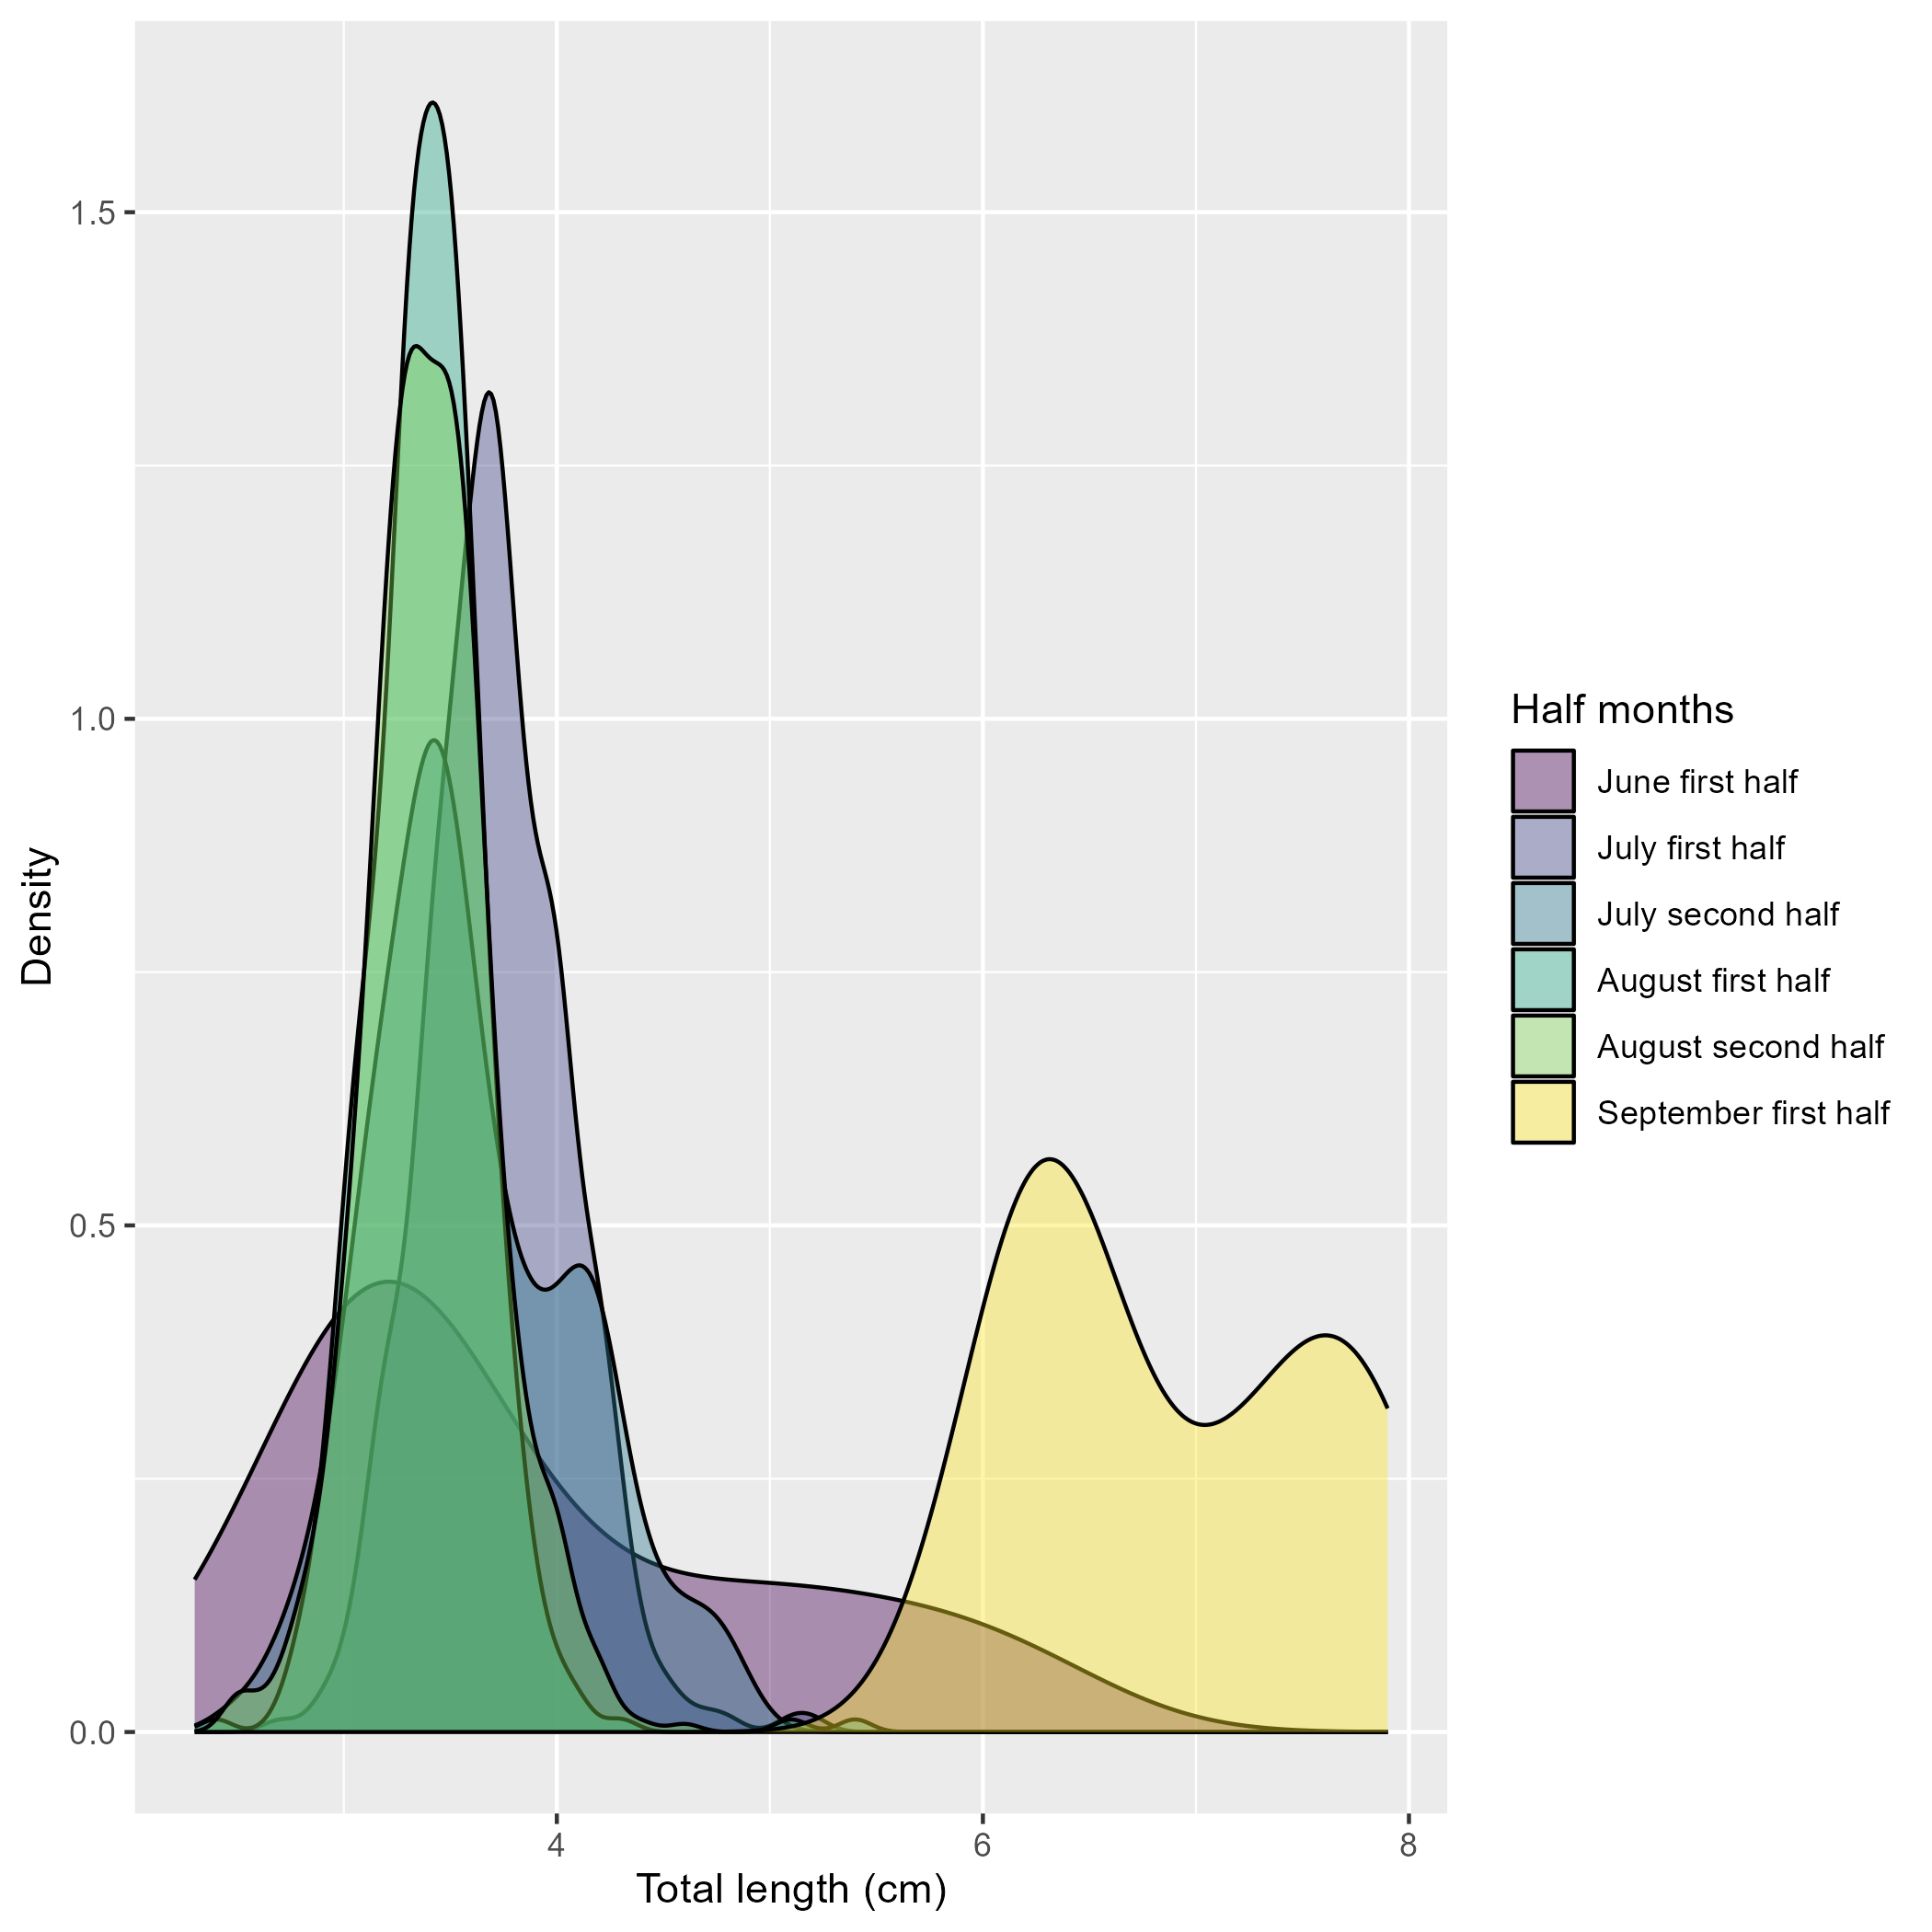
\includegraphics[width=1\textwidth,height=1\textheight]{C:/Assessments/2023/copper_rockfish_2023/documents/shared_figures/copper_length_by_half_month.png}
\caption{Distribution of YOY copper rockfish lengths from fish genetically identified from D. Baetscher.\label{fig:copper-smurf-length}}
\end{figure}

\pagebreak

\begin{figure}
\centering
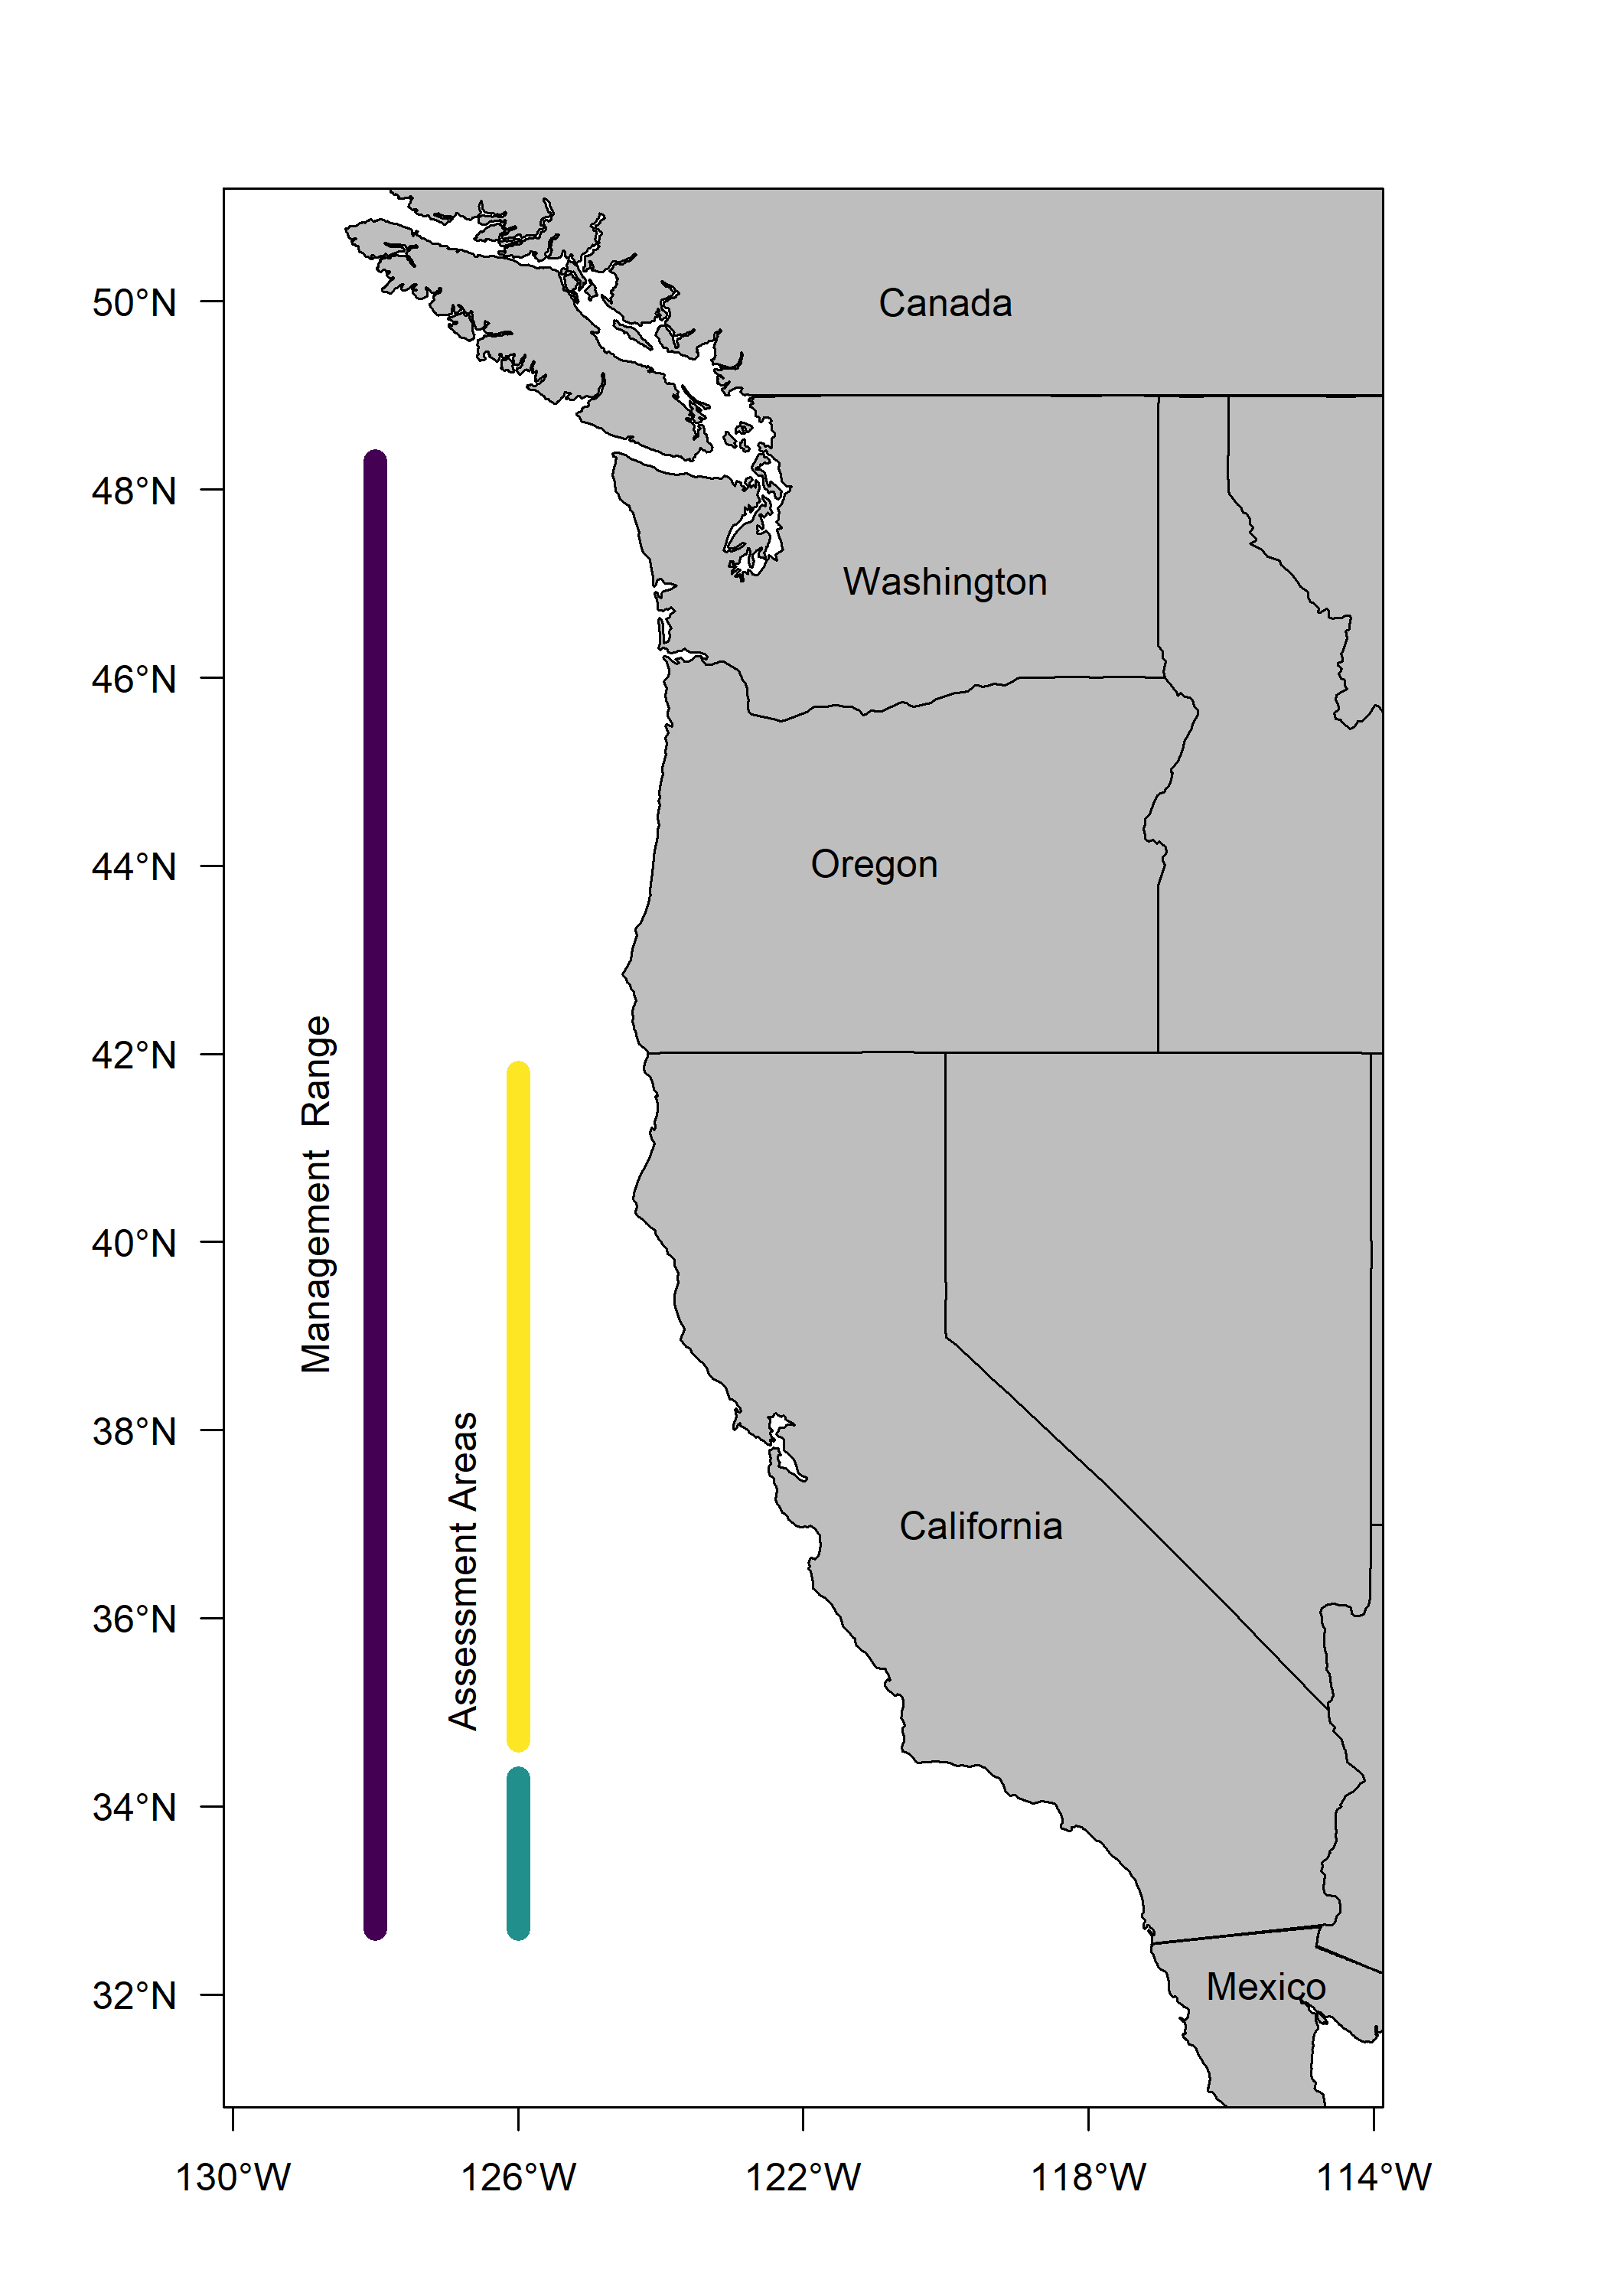
\includegraphics[width=1\textwidth,height=1\textheight]{C:/Assessments/2023/copper_rockfish_2023/documents/shared_figures/map.png}
\caption{Map of management area and the 2023 assessments areas for copper rockfish.\label{fig:ca-map}}
\end{figure}

\pagebreak

\begin{figure}
\centering
\includegraphics[width=1\textwidth,height=1\textheight]{N:/Assessments/CurrentAssessments/copper_rockfish_2023/models/sca/14.0_base_forecast/plots/catch2 landings stacked.png}
\caption{Landings by fleet used in the base model where catches in metric tons by fleet are stacked.\label{fig:catch}}
\end{figure}

\pagebreak

\begin{figure}
\centering
\includegraphics[width=1\textwidth,height=1\textheight]{N:/Assessments/CurrentAssessments/copper_rockfish_2023/models/sca/14.0_base_forecast/plots/data_plot.png}
\caption{Summary of data sources used in the base model.\label{fig:data-plot}}
\end{figure}

\pagebreak

\begin{figure}
\centering
\includegraphics[width=1\textwidth,height=1\textheight]{N:/Assessments/CurrentAssessments/copper_rockfish_2023/models/sca/14.0_base_forecast/plots/comp_lendat_bubflt1mkt0.png}
\caption{Length composition data from the commercial dead fleet.\label{fig:com-dead-len-data}}
\end{figure}

\pagebreak

\begin{figure}
\centering
\includegraphics[width=1\textwidth,height=1\textheight]{N:/Assessments/CurrentAssessments/copper_rockfish_2023/models/sca/14.0_base_forecast/plots/comp_lendat_data_weighting_TA1.8_Commercial_dead.png}
\caption{Mean length for commercial dead fleet with 95 percent confidence intervals.\label{fig:mean-com-dead-len-data}}
\end{figure}

\pagebreak

\begin{figure}
\centering
\includegraphics[width=1\textwidth,height=1\textheight]{N:/Assessments/CurrentAssessments/copper_rockfish_2023/models/sca/14.0_base_forecast/plots/comp_lendat_data_weighting_TA1.8_Commercial_dead.png}
\caption{Age composition data from the commercial dead and recreational CPFV fleets. The commercial samples were all from 2022 and the CPFV samples were all from 1975.\label{fig:com-dead-age-data}}
\end{figure}

\pagebreak

\begin{figure}
\centering
\includegraphics[width=1\textwidth,height=1\textheight]{N:/Assessments/CurrentAssessments/copper_rockfish_2023/data/ages/plots/coop_crfs_length_comparison.png}
\caption{Comparison of all length collected by the CRFS sampling program for the CPFV fleet to the lengths from the fish with ages from the cooperative sampling program. The length distributions in the area north of Point Conception are in general agreement while the distribution of lengths collected by this program does not align with the length samples from CRFS.\label{fig:coop-len-comparison}}
\end{figure}

\pagebreak

\begin{figure}
\centering
\includegraphics[width=1\textwidth,height=1\textheight]{N:/Assessments/CurrentAssessments/copper_rockfish_2023/models/sca/14.0_base_forecast/plots/comp_lendat_bubflt2mkt0.png}
\caption{Length composition data from the commercial live fleet.\label{fig:com-live-len-data}}
\end{figure}

\pagebreak

\begin{figure}
\centering
\includegraphics[width=1\textwidth,height=1\textheight]{N:/Assessments/CurrentAssessments/copper_rockfish_2023/models/sca/14.0_base_forecast/plots/comp_lendat_data_weighting_TA1.8_Commercial_live.png}
\caption{Mean length for commercial live fleet with 95 percent confidence intervals.\label{fig:mean-com-live-len-data}}
\end{figure}

\pagebreak

\begin{figure}
\centering
\includegraphics[width=1\textwidth,height=1\textheight]{N:/Assessments/CurrentAssessments/copper_rockfish_2023/data/rec_indices/mrfss_cpfv_dockside/south/forSS/Index.png}
\caption{Estimated annual index of abundances for the CPFV fleet based on MRFSS survey data.\label{fig:mrfss-index-main}}
\end{figure}

\pagebreak

\begin{figure}
\centering
\includegraphics[width=1\textwidth,height=1\textheight]{N:/Assessments/CurrentAssessments/copper_rockfish_2023/data/rec_indices/crfs_cpfv_onboard/south/main_effects/Index.png}
\caption{Estimated annual index of abundances for the CPFV fleet based on CRFS survey data.\label{fig:crfs-index-main}}
\end{figure}

\pagebreak

\begin{figure}
\centering
\includegraphics[width=1\textwidth,height=1\textheight]{N:/Assessments/CurrentAssessments/copper_rockfish_2023/data/rec_indices/crfs_pr_dockside/south/rm_last2yrs/Index.png}
\caption{Estimated annual index of abundances for the CPFV fleet based on CRFS survey data.\label{fig:crfs-pr-index-main}}
\end{figure}

\pagebreak

\begin{figure}
\centering
\includegraphics[width=1\textwidth,height=1\textheight]{N:/Assessments/CurrentAssessments/copper_rockfish_2023/models/sca/14.0_base_forecast/plots/comp_lendat_bubflt3mkt0_page2.png}
\caption{Length composition data from the recreational CPFV fleet.\label{fig:rec-cpfv-len-data}}
\end{figure}

\pagebreak

\begin{figure}
\centering
\includegraphics[width=1\textwidth,height=1\textheight]{N:/Assessments/CurrentAssessments/copper_rockfish_2023/models/sca/14.0_base_forecast/plots/comp_lendat_data_weighting_TA1.8_Rec_CPFV.png}
\caption{Mean length for recreational CPFV fleet with 95 percent confidence intervals.\label{fig:mean-rec-cpfv-len-data}}
\end{figure}

\pagebreak

\begin{figure}
\centering
\includegraphics[width=1\textwidth,height=1\textheight]{N:/Assessments/CurrentAssessments/copper_rockfish_2023/models/sca/14.0_base_forecast/plots/comp_lendat_bubflt4mkt0_page2.png}
\caption{Length composition data from the recreation PR fleet.\label{fig:rec-pr-len-data}}
\end{figure}

\pagebreak

\begin{figure}
\centering
\includegraphics[width=1\textwidth,height=1\textheight]{N:/Assessments/CurrentAssessments/copper_rockfish_2023/models/sca/14.0_base_forecast/plots/comp_lendat_data_weighting_TA1.8_Rec_Private.png}
\caption{Mean length for recreational PR fleet with 95 percent confidence intervals.\label{fig:mean-rec-pr-len-data}}
\end{figure}

\pagebreak

\begin{figure}
\centering
\includegraphics[width=1\textwidth,height=1\textheight]{N:/Assessments/CurrentAssessments/copper_rockfish_2023/data/survey_indices/plots/south_survey_locations_designation.png}
\caption{Sample locations by each of the fishery-independent data sources used in the base model with indices of abundance, lengths, and ages if collected.\label{fig:survey-locations}}
\end{figure}

\pagebreak

\begin{figure}
\centering
\includegraphics[width=1\textwidth,height=1\textheight]{N:/Assessments/CurrentAssessments/copper_rockfish_2023/data/survey_indices/plots/south_survey_locations.png}
\caption{Sample locations by area, areas open to fishing (reference) and MPAS, for each of the fishery-independent data sources used in the base model with indices of abundance, lengths, and ages if collected.\label{fig:ref-mpa}}
\end{figure}

\pagebreak

\begin{figure}
\centering
\includegraphics[width=1\textwidth,height=1\textheight]{N:/Assessments/CurrentAssessments/copper_rockfish_2023/data/survey_indices/ccfrp/south/area_weighted/Index.png}
\caption{Estimated index of abundance from the CCFRP Hook and LIne survey.\label{fig:ccfrp-index-main}}
\end{figure}

\pagebreak

\begin{figure}
\centering
\includegraphics[width=1\textwidth,height=1\textheight]{N:/Assessments/CurrentAssessments/copper_rockfish_2023/models/sca/14.0_base_forecast/plots/comp_lendat_bubflt5mkt0.png}
\caption{Length composition data from the CCFRP Hook and Line survey.\label{fig:ccfrp-len-data}}
\end{figure}

\pagebreak

\begin{figure}
\centering
\includegraphics[width=1\textwidth,height=1\textheight]{N:/Assessments/CurrentAssessments/copper_rockfish_2023/models/sca/14.0_base_forecast/plots/comp_gstagedat_bubflt5mkt0.png}
\caption{Age composition data from the CCFRP Hook and Line survey.\label{fig:ccfrp-age-data}}
\end{figure}

\pagebreak

\begin{figure}
\centering
\includegraphics[width=1\textwidth,height=1\textheight]{N:/Assessments/CurrentAssessments/copper_rockfish_2023/models/sca/14.0_base_forecast/plots/comp_lendat_data_weighting_TA1.8_CCFRP.png}
\caption{Mean length for the CCFRP Hook and Line survey with 95 percent confidence intervals.\label{fig:ccfrp-mean-len-data}}
\end{figure}

\pagebreak

\begin{figure}
\centering
\includegraphics[width=1\textwidth,height=1\textheight]{N:/Assessments/CurrentAssessments/copper_rockfish_2023/data/survey_indices/nwfsc_hkl/maps/Map_HL_Sites_lndscp.jpg}
\caption{Area sampled by the NWFSC Hook and Line survey.\label{fig:nwfsc-hkl-map}}
\end{figure}

\pagebreak

\begin{figure}
\centering
\includegraphics[width=1\textwidth,height=1\textheight]{N:/Assessments/CurrentAssessments/copper_rockfish_2023/data/survey_indices/nwfsc_hkl/plots/hkl_copper_by_site_count_all_years.png}
\caption{Observations of copper rockfish by the NWFSC Hook and Line survey by sample area, inside and outside Cowcod Conservation areas (CCA).\label{fig:nwfsc-hkl-site}}
\end{figure}

\pagebreak

\begin{figure}
\centering
\includegraphics[width=1\textwidth,height=1\textheight]{N:/Assessments/CurrentAssessments/copper_rockfish_2023/data/survey_indices/nwfsc_hkl/plots/raw_cpue_nwfsc_hkl_by_mpa_vs_open_by_region.png}
\caption{Raw CPUE inside and outside protected areas by region sampled by the NWFSC Hook and Line survey.\label{fig:nwfsc-hkl-region-main}}
\end{figure}

\pagebreak

\begin{figure}
\centering
\includegraphics[width=1\textwidth,height=1\textheight]{N:/Assessments/CurrentAssessments/copper_rockfish_2023/data/survey_indices/nwfsc_hkl/plots/nwfsc_hkl_observations_by_depth.png}
\caption{Number of observations by depth (m) inside and outside the CCAs.\label{fig:nwfsc-hkl-depth}}
\end{figure}

\pagebreak

\begin{figure}
\centering
\includegraphics[width=1\textwidth,height=1\textheight]{N:/Assessments/CurrentAssessments/copper_rockfish_2023/data/survey_indices/nwfsc_hkl/glm_delta_lognormal_year_area_depth_drop_vermilion_bocaccio_all_areas_re_site_area_weighted/Index.png}
\caption{Estimated index of abundance for copper rockfish.\label{fig:nwfsc-hkl-index-main}}
\end{figure}

\pagebreak

\begin{figure}
\centering
\includegraphics[width=1\textwidth,height=1\textheight]{N:/Assessments/CurrentAssessments/copper_rockfish_2023/data/survey_indices/nwfsc_hkl/plots/hkl_observations_by_length_sex_area.png}
\caption{Observed length (cm) distribution of copper rockfish by the NWFSC Hook and Line survey by sample area, inside and outside Cowcod Conservation areas (CCA).\label{fig:nwfsc-hkl-site-len}}
\end{figure}

\pagebreak

\begin{figure}
\centering
\includegraphics[width=1\textwidth,height=1\textheight]{N:/Assessments/CurrentAssessments/copper_rockfish_2023/data/survey_indices/nwfsc_hkl/plots/nwfsc_hkl_age_at_length.png}
\caption{Age and length by sex for copper rockfish in the NWFSC Hook and Line survey.\label{fig:nwfsc-hkl-len-age}}
\end{figure}

\pagebreak

\begin{figure}
\centering
\includegraphics[width=1\textwidth,height=1\textheight]{N:/Assessments/CurrentAssessments/copper_rockfish_2023/models/sca/14.0_base_forecast/plots/comp_lendat_bubflt7mkt0.png}
\caption{Length composition data from the NWFSC Hook and Line survey.\label{fig:hkl-len-data}}
\end{figure}

\pagebreak

\begin{figure}
\centering
\includegraphics[width=1\textwidth,height=1\textheight]{N:/Assessments/CurrentAssessments/copper_rockfish_2023/models/sca/14.0_base_forecast/plots/comp_lendat_data_weighting_TA1.8_NWFSC_HKL.png}
\caption{Mean length for NWFSC Hook and Line survey with 95 percent confidence intervals.\label{fig:mean-hkl-len-data}}
\end{figure}

\pagebreak

\begin{figure}
\centering
\includegraphics[width=1\textwidth,height=1\textheight]{N:/Assessments/CurrentAssessments/copper_rockfish_2023/data/survey_indices/rov/plots/rov_transect_collapsed_copper_south_protection_count.png}
\caption{The location and size of observations across all years and transects.\label{fig:rov-obs-loc}}
\end{figure}

\pagebreak

\begin{figure}
\centering
\includegraphics[width=1\textwidth,height=1\textheight]{N:/Assessments/CurrentAssessments/copper_rockfish_2023/data/survey_indices/rov/plots/south_raw_cpue_by_mpa_group_by_year.png}
\caption{The trend of the calculated CPUE by each MPA and Reference group by year.\label{fig:rov-raw-cpue}}
\end{figure}

\pagebreak

\begin{figure}
\centering
\includegraphics[width=1\textwidth,height=1\textheight]{N:/Assessments/CurrentAssessments/copper_rockfish_2023/data/survey_indices/rov/plots/rov_length_by_area_designation_april_data.png}
\caption{The distribution of lengths across all years for MPA and Reference areas north and south of Point Conception.\label{fig:rov-len}}
\end{figure}

\pagebreak

\begin{figure}
\centering
\includegraphics[width=1\textwidth,height=1\textheight]{N:/Assessments/CurrentAssessments/copper_rockfish_2023/models/sca/14.0_base_forecast/plots/comp_lendat_bubflt6mkt0.png}
\caption{Length composition data from the CDFW ROV survey.\label{fig:rov-len-data}}
\end{figure}

\pagebreak

\begin{figure}
\centering
\includegraphics[width=1\textwidth,height=1\textheight]{N:/Assessments/CurrentAssessments/copper_rockfish_2023/models/sca/14.0_base_forecast/plots/comp_lendat_data_weighting_TA1.8_CDFW_ROV.png}
\caption{Mean length for the CDFW ROV survey with 95 percent confidence intervals.\label{fig:mean-rov-len-data}}
\end{figure}

\pagebreak

\begin{figure}
\centering
\includegraphics[width=1\textwidth,height=1\textheight]{N:/Assessments/CurrentAssessments/copper_rockfish_2023/models/sca/14.0_base_forecast/plots/index9_standcpueall.png}
\caption{Standardized indices overlaid with each index rescaled to have a mean observation equal to 1.0. Note, the MRFSS CPFV (Rec\_CPFV) fishery-dependent index of abundance was not fit in the model but is included here for illustration.\label{fig:stand-cpue}}
\end{figure}

\pagebreak

\begin{figure}
\centering
\includegraphics[width=1\textwidth,height=1\textheight]{N:/Assessments/CurrentAssessments/copper_rockfish_2023/models/sca/14.0_base_forecast/plots/comp_lendat_flt9mkt0.png}
\caption{Length distribution by year for fish sampled by the NWFSC WCGBT survey.\label{fig:growth-wcgbt-len}}
\end{figure}

\pagebreak

\begin{figure}
\centering
\includegraphics[width=1\textwidth,height=1\textheight]{N:/Assessments/CurrentAssessments/copper_rockfish_2023/models/sca/14.0_base_forecast/plots/comp_lendat_data_weighting_TA1.8_WCGBT_Growth.png}
\caption{Mean length distribution by year for fish sampled by the NWFSC WCGBT survey.\label{fig:growth-mean-wcgbt-len}}
\end{figure}

\pagebreak

\begin{figure}
\centering
\includegraphics[width=1\textwidth,height=1\textheight]{N:/Assessments/CurrentAssessments/copper_rockfish_2023/models/sca/14.0_base_forecast/plots/comp_lendat_flt10mkt0.png}
\caption{Length distribution by year for fish sampled by the Pearson Research study (2005-2007) and the CPFV cooperative collection program (2022).\label{fig:growth-coop-len}}
\end{figure}

\pagebreak

\begin{figure}
\centering
\includegraphics[width=1\textwidth,height=1\textheight]{N:/Assessments/CurrentAssessments/copper_rockfish_2023/models/sca/14.0_base_forecast/plots/comp_lendat_data_weighting_TA1.8_COOP_Growth.png}
\caption{Mean length distribution by year for fish sampled by the Pearson Research Program (2005-2007) and the CPFV cooperative colletion program (2022).\label{fig:growth-mean-coop-len}}
\end{figure}

\pagebreak

\begin{figure}
\centering
\includegraphics[width=1\textwidth,height=1\textheight]{N:/Assessments/CurrentAssessments/copper_rockfish_2023/data/ages/plots/south_growth_length_comparison.png}
\caption{Length distribution of fish by collection source that were used as conditional age-at-length data in the growth fleet.\label{fig:growth-len-dist}}
\end{figure}

\pagebreak

\begin{figure}
\centering
\includegraphics[width=1\textwidth,height=1\textheight]{N:/Assessments/CurrentAssessments/copper_rockfish_2023/data/ages/plots/south_growth_age_comparison.png}
\caption{Age distribution of fish by collection source that were used as conditional age-at-length data in the growth fleet.\label{fig:growth-age-dist}}
\end{figure}

\pagebreak

\begin{figure}
\centering
\includegraphics[width=1\textwidth,height=1\textheight]{N:/Assessments/CurrentAssessments/copper_rockfish_2023/data/wcgbt/south/plots/cpue_map.png}
\caption{Location and catch-per-unit-effort by location caught south of Point Conception by the NWFSC WCGBT survey.\label{fig:wcgbt-cpue}}
\end{figure}

\pagebreak

\begin{figure}
\centering
\includegraphics[width=1\textwidth,height=1\textheight]{N:/Assessments/CurrentAssessments/copper_rockfish_2023/data/wcgbt/south/plots/presence-absence_proportion_by_depth.png}
\caption{Number of positive tows across all years by depth in meters.\label{fig:wcgbt-depth}}
\end{figure}

\pagebreak

\begin{figure}
\centering
\includegraphics[width=1\textwidth,height=1\textheight]{N:/Assessments/CurrentAssessments/copper_rockfish_2023/data/wcgbt/plots/wcgbt_south_age_at_length_by_area.png}
\caption{Age and length by sex for copper rockfish caught south of Point Conception by the NWFSC WCGBT survey.\label{fig:wcgbt-len-age}}
\end{figure}

\pagebreak

\hypertarget{biology}{%
\subsection{Biology}\label{biology}}

\begin{figure}
\centering
\includegraphics[width=1\textwidth,height=1\textheight]{N:/Assessments/CurrentAssessments/copper_rockfish_2023/models/sca/14.0_base_forecast/plots/bio6_maturity.png}
\caption{Maturity as a function of length.\label{fig:maturity}}
\end{figure}

\pagebreak

\begin{figure}
\centering
\includegraphics[width=1\textwidth,height=1\textheight]{N:/Assessments/CurrentAssessments/copper_rockfish_2023/models/sca/14.0_base_forecast/plots/bio9_fecundity_len.png}
\caption{Fecundity as a function of length.\label{fig:fecundity}}
\end{figure}

\pagebreak

\begin{figure}
\centering
\includegraphics[width=1\textwidth,height=1\textheight]{N:/Assessments/CurrentAssessments/copper_rockfish_2023/data/wcgbt/plots/length_fraction_female.png}
\caption{Fraction of each sex by length by the NWFSC WCGBT survey.\label{fig:frac-sex-len}}
\end{figure}

\pagebreak

\begin{figure}
\centering
\includegraphics[width=1\textwidth,height=1\textheight]{N:/Assessments/CurrentAssessments/copper_rockfish_2023/data/biology/plots/Length_Weight_All.png}
\caption{Estimated weight-at-length.\label{fig:weight-length}}
\end{figure}

\pagebreak

\begin{figure}
\centering
\includegraphics[width=1\textwidth,height=1\textheight]{N:/Assessments/CurrentAssessments/copper_rockfish_2023/data/ages/ageing_error/B0_S3/Reader_1_vs_Reader_2.png}
\caption{Distribution of double reads between age reader 1 and 2.\label{fig:age-error-dist}}
\end{figure}

\pagebreak

\begin{figure}
\centering
\includegraphics[width=1\textwidth,height=1\textheight]{N:/Assessments/CurrentAssessments/copper_rockfish_2023/models/sca/14.0_base_forecast/plots/numbers5_ageerrorSD.png}
\caption{Ageing imprecision standard deviation of observed age in years.\label{fig:age-error}}
\end{figure}

\pagebreak

\begin{figure}
\centering
\includegraphics[width=1\textwidth,height=1\textheight]{N:/Assessments/CurrentAssessments/copper_rockfish_2023/models/sca/14.0_base_forecast/plots/numbers10_ageerror_matrix_1.png}
\caption{Distribution of observed age at true age for ageing error type 1.\label{fig:age-error-matrix}}
\end{figure}

\pagebreak

\hypertarget{model-results}{%
\subsection{Model Results}\label{model-results}}

\hypertarget{bridging}{%
\subsubsection{Bridging}\label{bridging}}

\begin{figure}
\centering
\includegraphics[width=1\textwidth,height=1\textheight]{N:/Assessments/CurrentAssessments/copper_rockfish_2023/models/sca/_bridging/_plots/0_model_convert_compare2_spawnbio_uncertainty.png}
\caption{Model version bridge comparison of estimated spawning output.\label{fig:bridge-ssb}}
\end{figure}

\pagebreak

\begin{figure}
\centering
\includegraphics[width=1\textwidth,height=1\textheight]{N:/Assessments/CurrentAssessments/copper_rockfish_2023/models/sca/_bridging/_plots/0_model_convert_compare4_Bratio_uncertainty.png}
\caption{Model version bridge comparison of estimated fraction unfished.\label{fig:bridge-depl}}
\end{figure}

\pagebreak

\begin{figure}
\centering
\includegraphics[width=1\textwidth,height=1\textheight]{N:/Assessments/CurrentAssessments/copper_rockfish_2023/models/sca/_bridging/_plots/full_bridge_1_compare2_spawnbio_uncertainty.png}
\caption{Model structure and data bridging comparison of estimated spawning output.\label{fig:data-bridge-ssb-1}}
\end{figure}

\pagebreak

\begin{figure}
\centering
\includegraphics[width=1\textwidth,height=1\textheight]{N:/Assessments/CurrentAssessments/copper_rockfish_2023/models/sca/_bridging/_plots/full_bridge_1_compare4_Bratio_uncertainty.png}
\caption{Model structure and data bridging comparison of estimated fraction unfished.\label{fig:data-bridge-depl-1}}
\end{figure}

\pagebreak

\begin{figure}
\centering
\includegraphics[width=1\textwidth,height=1\textheight]{N:/Assessments/CurrentAssessments/copper_rockfish_2023/models/sca/_bridging/_plots/full_bridge_2_compare2_spawnbio_uncertainty.png}
\caption{Model structure and data bridging comparison of estimated spawning output.\label{fig:data-bridge-ssb-2}}
\end{figure}

\pagebreak

\begin{figure}
\centering
\includegraphics[width=1\textwidth,height=1\textheight]{N:/Assessments/CurrentAssessments/copper_rockfish_2023/models/sca/_bridging/_plots/full_bridge_2_compare4_Bratio_uncertainty.png}
\caption{Model structure and data bridging comparison of estimated fraction unfished.\label{fig:data-bridge-depl-2}}
\end{figure}

\pagebreak

\begin{figure}
\centering
\includegraphics[width=1\textwidth,height=1\textheight]{N:/Assessments/CurrentAssessments/copper_rockfish_2023/management/fishing_regs.png}
\caption{The CDFW recreational season lenght and depth restriction for nearshore rockfish by month from 2000 to 2003. A triangle indicates a regulation change mid-month. The regions defined base on the following latitudes: Northern , Mendocino , San Francisco, Central , Southern. Not all management areas have been consistently defined over time. The northern and southern management areas have remained the same.\label{fig:depth-closures}}
\end{figure}

\pagebreak

\hypertarget{biology-1}{%
\subsubsection{Biology}\label{biology-1}}

\begin{figure}
\centering
\includegraphics[width=1\textwidth,height=1\textheight]{N:/Assessments/CurrentAssessments/copper_rockfish_2023/models/sca/14.0_base_forecast/plots/bio5_weightatsize.png}
\caption{Assumed weight-length relationship for each sex.\label{fig:est-len-wght}}
\end{figure}

\pagebreak

\begin{figure}
\centering
\includegraphics[width=1\textwidth,height=1\textheight]{N:/Assessments/CurrentAssessments/copper_rockfish_2023/models/sca/14.0_base_forecast/plots/bio1_sizeatage.png}
\caption{Model estimated length-at-age in the beginning of the year. Shaded area indicates 95 percent distribution of length-at-age around the estimated growth curve.\label{fig:mod-est-len-age}}
\end{figure}

\pagebreak

\hypertarget{selectivity}{%
\subsubsection{Selectivity}\label{selectivity}}

\begin{figure}
\centering
\includegraphics[width=1\textwidth,height=1\textheight]{N:/Assessments/CurrentAssessments/copper_rockfish_2023/models/sca/14.0_base_forecast/plots/south_selectivity.png}
\caption{Estimated selectivity for each fleet and survey in the base model.\label{fig:est-selex}}
\end{figure}

\newpage

\hypertarget{recruitment-1}{%
\subsubsection{Recruitment}\label{recruitment-1}}

\begin{figure}
\centering
\includegraphics[width=1\textwidth,height=1\textheight]{N:/Assessments/CurrentAssessments/copper_rockfish_2023/models/sca/14.0_base_forecast/plots/ts11_Age-0_recruits_(1000s)_with_95_asymptotic_intervals.png}
\caption{Estimated time series of age-0 recruits (1000s).\label{fig:recruits}}
\end{figure}

\pagebreak

\begin{figure}
\centering
\includegraphics[width=1\textwidth,height=1\textheight]{N:/Assessments/CurrentAssessments/copper_rockfish_2023/models/sca/14.0_base_forecast/plots/recdevs2_withbars.png}
\caption{Estimated time series of recruitment deviations.\label{fig:rec-devs}}
\end{figure}

\pagebreak

\begin{figure}
\centering
\includegraphics[width=1\textwidth,height=1\textheight]{N:/Assessments/CurrentAssessments/copper_rockfish_2023/models/sca/14.0_base_forecast/plots/SR_curve.png}
\caption{Stock-recruit curve. Point colors indicate year, with warmer colors indicating earlier years and cooler colors in showing later years.\label{fig:bh-curve}}
\end{figure}

\pagebreak

\begin{figure}
\centering
\includegraphics[width=1\textwidth,height=1\textheight]{N:/Assessments/CurrentAssessments/copper_rockfish_2023/models/sca/14.0_base_forecast/plots/recruit_fit_bias_adjust.png}
\caption{Points are transformed variances. Red line shows current settings for bias adjustment specified in control file. Blue line shows least squares estimate of alternative bias adjustment relationship for recruitment deviations (which may or may not be an improvement).\label{fig:bias-adjust}}
\end{figure}

\newpage

\hypertarget{fits-to-data}{%
\subsubsection{Fits to Data}\label{fits-to-data}}

\begin{figure}
\centering
\includegraphics[width=1\textwidth,height=1\textheight]{N:/Assessments/CurrentAssessments/copper_rockfish_2023/models/sca/14.0_base_forecast/plots/comp_lenfit__aggregated_across_time.png}
\caption{Length composition aggregated across years by fleet with the model estimated fit to the data by sex (green unsexed, red female, and blue male).\label{fig:len-agg-fit}}
\end{figure}

\pagebreak

\begin{figure}
\centering
\includegraphics[width=1\textwidth,height=1\textheight]{N:/Assessments/CurrentAssessments/copper_rockfish_2023/models/sca/14.0_base_forecast/plots/comp_lenfit_residsflt1mkt0.png}
\caption{Pearson residuals for commercial fleet. Closed bubble are positive residuals (observed \textgreater{} expected) and open bubbles are negative residuals (observed \textless{} expected).\label{fig:com-dead-pearson}}
\end{figure}

\pagebreak

\begin{figure}
\centering
\includegraphics[width=1\textwidth,height=1\textheight]{N:/Assessments/CurrentAssessments/copper_rockfish_2023/models/sca/14.0_base_forecast/plots/comp_lenfit_data_weighting_TA1.8_Commercial_dead.png}
\caption{Mean length for commercial dead lengths with 95 percent confidence intervals based on current samples sizes.\label{fig:com-dead-mean-len-fit}}
\end{figure}

\pagebreak

\begin{figure}
\centering
\includegraphics[width=1\textwidth,height=1\textheight]{N:/Assessments/CurrentAssessments/copper_rockfish_2023/models/sca/14.0_base_forecast/plots/comp_agefit__aggregated_across_time.png}
\caption{Age composition data aggregated across time by fleet.\label{fig:agg-marg-age-fit}}
\end{figure}

\pagebreak

\begin{figure}
\centering
\includegraphics[width=1\textwidth,height=1\textheight]{N:/Assessments/CurrentAssessments/copper_rockfish_2023/models/sca/14.0_base_forecast/plots/comp_agefit_residsflt1mkt0.png}
\caption{Pearson residuals for commercial dead age data. Closed bubble are positive residuals (observed \textgreater{} expected) and open bubbles are negative residuals (observed \textless{} expected).\label{fig:com-dead-age-pearson}}
\end{figure}

\pagebreak

\begin{figure}
\centering
\includegraphics[width=1\textwidth,height=1\textheight]{N:/Assessments/CurrentAssessments/copper_rockfish_2023/models/sca/14.0_base_forecast/plots/comp_lenfit_residsflt2mkt0.png}
\caption{Pearson residuals for commercial live fleet. Closed bubble are positive residuals (observed \textgreater{} expected) and open bubbles are negative residuals (observed \textless{} expected).\label{fig:com-live-pearson}}
\end{figure}

\pagebreak

\begin{figure}
\centering
\includegraphics[width=1\textwidth,height=1\textheight]{N:/Assessments/CurrentAssessments/copper_rockfish_2023/models/sca/14.0_base_forecast/plots/comp_lenfit_data_weighting_TA1.8_Commercial_live.png}
\caption{Mean length for commercial live fish lengths with 95 percent confidence intervals based on current samples sizes.\label{fig:com-live-mean-len-fit}}
\end{figure}

\pagebreak

\begin{figure}
\centering
\includegraphics[width=1\textwidth,height=1\textheight]{N:/Assessments/CurrentAssessments/copper_rockfish_2023/models/sca/14.0_base_forecast/plots/comp_lenfit_residsflt3mkt0_page2.png}
\caption{Pearson residuals for recreational CPFV fleet. Closed bubble are positive residuals (observed \textgreater{} expected) and open bubbles are negative residuals (observed \textless{} expected).\label{fig:rec-cpfv-pearson}}
\end{figure}

\pagebreak

\begin{figure}
\centering
\includegraphics[width=1\textwidth,height=1\textheight]{N:/Assessments/CurrentAssessments/copper_rockfish_2023/models/sca/14.0_base_forecast/plots/comp_lenfit_data_weighting_TA1.8_Rec_CPFV.png}
\caption{Mean length for recreational CPFV lengths with 95 percent confidence intervals based on current samples sizes.\label{fig:rec-cpfv-mean-len-fit}}
\end{figure}

\pagebreak

\begin{figure}
\centering
\includegraphics[width=1\textwidth,height=1\textheight]{N:/Assessments/CurrentAssessments/copper_rockfish_2023/data/rec_bds/plots/rec_south_ggridges_lengths_cpfv_district.png}
\caption{Length distributions observed in the CPFV fleet by CDFW district 1 (South) and 2 (Channel) since 2004.\label{fig:rec-cpfv-dist}}
\end{figure}

\pagebreak

\begin{figure}
\centering
\includegraphics[width=1\textwidth,height=1\textheight]{N:/Assessments/CurrentAssessments/copper_rockfish_2023/models/sca/14.0_base_forecast/plots/comp_agefit_residsflt3mkt0.png}
\caption{Pearson residuals for recreational CPFV age data. Closed bubble are positive residuals (observed \textgreater{} expected) and open bubbles are negative residuals (observed \textless{} expected).\label{fig:rec-cpfv-age-pearson}}
\end{figure}

\pagebreak

\begin{figure}
\centering
\includegraphics[width=1\textwidth,height=1\textheight]{N:/Assessments/CurrentAssessments/copper_rockfish_2023/models/sca/14.0_base_forecast/plots/comp_lenfit_residsflt4mkt0_page2.png}
\caption{Pearson residuals for recreational private/rental fleet. Closed bubble are positive residuals (observed \textgreater{} expected) and open bubbles are negative residuals (observed \textless{} expected).\label{fig:rec-pr-pearson}}
\end{figure}

\pagebreak

\begin{figure}
\centering
\includegraphics[width=1\textwidth,height=1\textheight]{N:/Assessments/CurrentAssessments/copper_rockfish_2023/models/sca/14.0_base_forecast/plots/comp_lenfit_data_weighting_TA1.8_Rec_Private.png}
\caption{Mean length for recreational private/rental lengths with 95 percent confidence intervals based on current samples sizes.\label{fig:rec-pr-mean-len-fit}}
\end{figure}

\pagebreak

\begin{figure}
\centering
\includegraphics[width=1\textwidth,height=1\textheight]{N:/Assessments/CurrentAssessments/copper_rockfish_2023/models/sca/14.0_base_forecast/plots/comp_lenfit_residsflt5mkt0.png}
\caption{Pearson residuals for CCFRP Hook and Line survey length data. Closed bubble are positive residuals (observed \textgreater{} expected) and open bubbles are negative residuals (observed \textless{} expected).\label{fig:ccfrp-len-pearson}}
\end{figure}

\pagebreak

\begin{figure}
\centering
\includegraphics[width=1\textwidth,height=1\textheight]{N:/Assessments/CurrentAssessments/copper_rockfish_2023/models/sca/14.0_base_forecast/plots/comp_lenfit_data_weighting_TA1.8_CCFRP.png}
\caption{Mean length for CCFRP Hook and Line survey lengths with 95 percent confidence intervals based on current samples sizes.\label{fig:ccfrp-mean-len-fit}}
\end{figure}

\pagebreak

\begin{figure}
\centering
\includegraphics[width=1\textwidth,height=1\textheight]{N:/Assessments/CurrentAssessments/copper_rockfish_2023/models/sca/14.0_base_forecast/plots/comp_condAAlfit_residsflt5mkt0.png}
\caption{Pearson residuals for CCFRP Hook and Line survey conditional-age-at-length data. Closed bubble are positive residuals (observed \textgreater{} expected) and open bubbles are negative residuals (observed \textless{} expected).\label{fig:ccfrp-age-pearson}}
\end{figure}

\pagebreak

\begin{figure}
\centering
\includegraphics[width=1\textwidth,height=1\textheight]{N:/Assessments/CurrentAssessments/copper_rockfish_2023/models/sca/14.0_base_forecast/plots/comp_lenfit_residsflt6mkt0.png}
\caption{Pearson residuals for CDFW ROV survey length data. Closed bubble are positive residuals (observed \textgreater{} expected) and open bubbles are negative residuals (observed \textless{} expected).\label{fig:rov-pearson}}
\end{figure}

\pagebreak

\begin{figure}
\centering
\includegraphics[width=1\textwidth,height=1\textheight]{N:/Assessments/CurrentAssessments/copper_rockfish_2023/models/sca/14.0_base_forecast/plots/comp_lenfit_data_weighting_TA1.8_CDFW_ROV.png}
\caption{Mean length for CDFW ROV survey lengths with 95 percent confidence intervals based on current samples sizes.\label{fig:rov-mean-len-fit}}
\end{figure}

\pagebreak

\begin{figure}
\centering
\includegraphics[width=1\textwidth,height=1\textheight]{N:/Assessments/CurrentAssessments/copper_rockfish_2023/models/sca/14.0_base_forecast/plots/comp_lenfit_residsflt7mkt0.png}
\caption{Pearson residuals for NWFSC Hook and Line survey length data. Closed bubble are positive residuals (observed \textgreater{} expected) and open bubbles are negative residuals (observed \textless{} expected).\label{fig:nwfsc-hkl-pearson}}
\end{figure}

\pagebreak

\begin{figure}
\centering
\includegraphics[width=1\textwidth,height=1\textheight]{N:/Assessments/CurrentAssessments/copper_rockfish_2023/models/sca/14.0_base_forecast/plots/comp_lenfit_data_weighting_TA1.8_NWFSC_HKL.png}
\caption{Mean length for NWFSC Hook and Line survey lengths with 95 percent confidence intervals based on current samples sizes.\label{fig:nwfsc-hkl-mean-len-fit}}
\end{figure}

\pagebreak

\begin{figure}
\centering
\includegraphics[width=1\textwidth,height=1\textheight]{N:/Assessments/CurrentAssessments/copper_rockfish_2023/models/sca/14.0_base_forecast/plots/comp_condAALfit_residsflt7mkt0_page1.png}
\caption{Pearson residuals for NWFSC Hook and Line survey conditional-age-at-length data. Closed bubble are positive residuals (observed \textgreater{} expected) and open bubbles are negative residuals (observed \textless{} expected).\label{fig:nwfsc-hkl-age-pearson-1}}
\end{figure}

\pagebreak

\begin{figure}
\centering
\includegraphics[width=1\textwidth,height=1\textheight]{N:/Assessments/CurrentAssessments/copper_rockfish_2023/models/sca/14.0_base_forecast/plots/comp_condAALfit_residsflt7mkt0_page2.png}
\caption{Pearson residuals for NWFSC Hook and Line survey conditional-age-at-length data. Closed bubble are positive residuals (observed \textgreater{} expected) and open bubbles are negative residuals (observed \textless{} expected).\label{fig:nwfsc-hkl-age-pearson-2}}
\end{figure}

\pagebreak

\begin{figure}
\centering
\includegraphics[width=1\textwidth,height=1\textheight]{N:/Assessments/CurrentAssessments/copper_rockfish_2023/models/sca/14.0_base_forecast/plots/comp_condAALfit_residsflt7mkt0_page3.png}
\caption{Pearson residuals for NWFSC Hook and Line survey conditional-age-at-length data. Closed bubble are positive residuals (observed \textgreater{} expected) and open bubbles are negative residuals (observed \textless{} expected).\label{fig:nwfsc-hkl-age-pearson-3}}
\end{figure}

\pagebreak

\begin{figure}
\centering
\includegraphics[width=1\textwidth,height=1\textheight]{N:/Assessments/CurrentAssessments/copper_rockfish_2023/models/sca/14.0_base_forecast/plots/comp_condAALfit_data_weighting_TA1.8_condAgeNWFSC_HKL.png}
\caption{Mean age for NWFSC Hook and Line survey age data with 95 percent confidence intervals based on current samples sizes.\label{fig:nwfsc-hkl-mean-age-fit}}
\end{figure}

\pagebreak

\begin{figure}
\centering
\includegraphics[width=1\textwidth,height=1\textheight]{N:/Assessments/CurrentAssessments/copper_rockfish_2023/models/sca/14.0_base_forecast/plots/comp_lenfit_residsflt9mkt0.png}
\caption{Pearson residuals for NWFSC WCGBT survey fleet length data. Closed bubble are positive residuals (observed \textgreater{} expected) and open bubbles are negative residuals (observed \textless{} expected).\label{fig:wcgbt-len-pearson}}
\end{figure}

\pagebreak

\begin{figure}
\centering
\includegraphics[width=1\textwidth,height=1\textheight]{N:/Assessments/CurrentAssessments/copper_rockfish_2023/models/sca/14.0_base_forecast/plots/comp_lenfit_data_weighting_TA1.8_WCGBT_Growth.png}
\caption{Mean length for the NWFSC WCGBT survey lengths with 95 percent confidence intervals based on current samples sizes.\label{fig:wcgbt-mean-len-fit}}
\end{figure}

\pagebreak

\begin{figure}
\centering
\includegraphics[width=1\textwidth,height=1\textheight]{N:/Assessments/CurrentAssessments/copper_rockfish_2023/models/sca/14.0_base_forecast/plots/comp_condAALfit_residsflt9mkt0_page1.png}
\caption{Pearson residuals for the NWFSC WCGBT survey conditional-age-at-length data. Closed bubble are positive residuals (observed \textgreater{} expected) and open bubbles are negative residuals (observed \textless{} expected).\label{fig:wcgbt-age-pearson-1}}
\end{figure}

\pagebreak

\begin{figure}
\centering
\includegraphics[width=1\textwidth,height=1\textheight]{N:/Assessments/CurrentAssessments/copper_rockfish_2023/models/sca/14.0_base_forecast/plots/comp_condAALfit_residsflt9mkt0_page2.png}
\caption{Pearson residuals for the NWFSC WCGBT survey conditional-age-at-length data. Closed bubble are positive residuals (observed \textgreater{} expected) and open bubbles are negative residuals (observed \textless{} expected).\label{fig:wcgbt-age-pearson-2}}
\end{figure}

\pagebreak

\begin{figure}
\centering
\includegraphics[width=1\textwidth,height=1\textheight]{N:/Assessments/CurrentAssessments/copper_rockfish_2023/models/sca/14.0_base_forecast/plots/comp_condAALfit_residsflt9mkt0_page3.png}
\caption{Pearson residuals for the NWFSC WCGBT survey conditional-age-at-length data. Closed bubble are positive residuals (observed \textgreater{} expected) and open bubbles are negative residuals (observed \textless{} expected).\label{fig:wcgbt-age-pearson-3}}
\end{figure}

\pagebreak

\begin{figure}
\centering
\includegraphics[width=1\textwidth,height=1\textheight]{N:/Assessments/CurrentAssessments/copper_rockfish_2023/models/sca/14.0_base_forecast/plots/comp_condAALfit_data_weighting_TA1.8_condAgeWCGBT_Growth.png}
\caption{Mean age for the NWFSC WCGBT survey age data with 95 percent confidence intervals based on current samples sizes.\label{fig:wcgbt-mean-age-fit}}
\end{figure}

\pagebreak

\begin{figure}
\centering
\includegraphics[width=1\textwidth,height=1\textheight]{N:/Assessments/CurrentAssessments/copper_rockfish_2023/models/sca/14.0_base_forecast/plots/comp_lenfit_residsflt10mkt0.png}
\caption{Pearson residuals for Pearson and CPFV cooperative collection length data. Closed bubble are positive residuals (observed \textgreater{} expected) and open bubbles are negative residuals (observed \textless{} expected).\label{fig:coop-len-pearson}}
\end{figure}

\pagebreak

\begin{figure}
\centering
\includegraphics[width=1\textwidth,height=1\textheight]{N:/Assessments/CurrentAssessments/copper_rockfish_2023/models/sca/14.0_base_forecast/plots/comp_lenfit_data_weighting_TA1.8_COOP_Growth.png}
\caption{Mean length for the Pearson and CPFV cooperative collection lengths with 95 percent confidence intervals based on current samples sizes.\label{fig:coop-mean-len-fit}}
\end{figure}

\pagebreak

\begin{figure}
\centering
\includegraphics[width=1\textwidth,height=1\textheight]{N:/Assessments/CurrentAssessments/copper_rockfish_2023/models/sca/14.0_base_forecast/plots/comp_condAALfit_residsflt10mkt0.png}
\caption{Pearson residuals for the Pearson and CPFV cooperative collection conditional-age-at-length data. Closed bubble are positive residuals (observed \textgreater{} expected) and open bubbles are negative residuals (observed \textless{} expected).\label{fig:coop-age-pearson}}
\end{figure}

\pagebreak

\begin{figure}
\centering
\includegraphics[width=1\textwidth,height=1\textheight]{N:/Assessments/CurrentAssessments/copper_rockfish_2023/models/sca/14.0_base_forecast/plots/comp_condAALfit_data_weighting_TA1.8_condAgeCOOP_Growth.png}
\caption{Mean age for the Pearson and CPFV cooperative collection age data with 95 percent confidence intervals based on current samples sizes.\label{fig:coop-mean-age-fit}}
\end{figure}

\pagebreak

\begin{figure}
\centering
\includegraphics[width=1\textwidth,height=1\textheight]{N:/Assessments/CurrentAssessments/copper_rockfish_2023/models/sca/14.0_base_forecast/plots/index5_logcpuefit_CRFS_CPFV.png}
\caption{Fit to log index data on log scale for the recreational CRFS CPFV index of abundance. Lines indicate 95\% uncertainty interval around index values based on the model assumption of lognormal error. Thicker lines indicate input uncertainty before addition of estimated additional uncertainty parameter.\label{fig:crfs-cpfv-index-fit}}
\end{figure}

\pagebreak

\begin{figure}
\centering
\includegraphics[width=1\textwidth,height=1\textheight]{N:/Assessments/CurrentAssessments/copper_rockfish_2023/models/sca/14.0_base_forecast/plots/index5_logcpuefit_Rec_Private.png}
\caption{Fit to log index data on log scale for the recreational private index of abundance. Lines indicate 95\% uncertainty interval around index values based on the model assumption of lognormal error. Thicker lines indicate input uncertainty before addition of estimated additional uncertainty parameter.\label{fig:crfs-pr-index-fit}}
\end{figure}

\pagebreak

\begin{figure}
\centering
\includegraphics[width=1\textwidth,height=1\textheight]{N:/Assessments/CurrentAssessments/copper_rockfish_2023/models/sca/14.0_base_forecast/plots/index5_logcpuefit_CCFRP.png}
\caption{Fit to log index data on log scale for the CCFRP Hook and Line survey index of abundance. Lines indicate 95\% uncertainty interval around index values based on the model assumption of lognormal error. Thicker lines indicate input uncertainty before addition of estimated additional uncertainty parameter.\label{fig:ccfrp-index-fit}}
\end{figure}

\pagebreak

\begin{figure}
\centering
\includegraphics[width=1\textwidth,height=1\textheight]{N:/Assessments/CurrentAssessments/copper_rockfish_2023/models/sca/14.0_base_forecast/plots/index5_logcpuefit_CDFW_ROV.png}
\caption{Fit to log index data on log scale for the CDFW ROV index of abundance. Lines indicate 95\% uncertainty interval around index values based on the model assumption of lognormal error. Thicker lines indicate input uncertainty before addition of estimated additional uncertainty parameter.\label{fig:rov-index-fit}}
\end{figure}

\pagebreak

\begin{figure}
\centering
\includegraphics[width=1\textwidth,height=1\textheight]{N:/Assessments/CurrentAssessments/copper_rockfish_2023/models/sca/14.0_base_forecast/plots/index5_logcpuefit_NWFSC_HKL.png}
\caption{Fit to log index data on log scale for the NWFSC Hook and Line index of abundance. Lines indicate 95\% uncertainty interval around index values based on the model assumption of lognormal error. Thicker lines indicate input uncertainty before addition of estimated additional uncertainty parameter.\label{fig:nwfsc-hkl-index-fit}}
\end{figure}

\pagebreak

\hypertarget{time-series}{%
\subsubsection{Time-series}\label{time-series}}

\begin{figure}
\centering
\includegraphics[width=1\textwidth,height=1\textheight]{N:/Assessments/CurrentAssessments/copper_rockfish_2023/models/sca/14.0_base_forecast/plots/ts7_Spawning_output_with_95_asymptotic_intervals_intervals.png}
\caption{Estimated time series of spawning output for the area south of Point Conception in California.\label{fig:ssb}}
\end{figure}

\pagebreak

\begin{figure}
\centering
\includegraphics[width=1\textwidth,height=1\textheight]{N:/Assessments/CurrentAssessments/copper_rockfish_2023/models/sca/14.0_base_forecast/plots/ts1_Total_biomass_(mt).png}
\caption{Estimated time series of total biomass for the area south of Point Conception in California.\label{fig:tot-bio}}
\end{figure}

\pagebreak

\begin{figure}
\centering
\includegraphics[width=1\textwidth,height=1\textheight]{N:/Assessments/CurrentAssessments/copper_rockfish_2023/models/sca/14.0_base_forecast/plots/ts9_Relative_spawning_output_intervals.png}
\caption{Estimated time series of relative spawning output for the area south of Point Conception in California.\label{fig:depl}}
\end{figure}

\pagebreak

\begin{figure}
\centering
\includegraphics[width=1\textwidth,height=1\textheight]{C:/Assessments/2023/copper_rockfish_2023/documents/shared_figures/spawning_output_combined.png}
\caption{Estimated combined time series of spawning output for copper rockfish in California waters.\label{fig:sb-all}}
\end{figure}

\clearpage

\begin{figure}
\centering
\includegraphics[width=1\textwidth,height=1\textheight]{C:/Assessments/2023/copper_rockfish_2023/documents/shared_figures/depletion_combined.png}
\caption{Estimated combined time series of relative spawning output for copper rockfish in California waters.\label{fig:depl-all}}
\end{figure}

\clearpage

\hypertarget{sensitivity-analyses-and-retrospectives}{%
\subsubsection{Sensitivity Analyses and Retrospectives}\label{sensitivity-analyses-and-retrospectives}}

\begin{figure}
\centering
\includegraphics[width=1\textwidth,height=1\textheight]{N:/Assessments/CurrentAssessments/copper_rockfish_2023/models/sca/_sensitivities/_plots/Sensi_REplot_all_horizontal.png}
\caption{Comparison of the relative change in estimated management quantities as compared to the base model. The quantities compared are the estimate of unfished spawning biomass (SB0), spawning output in 2023 (SB2023), the relative spawnin output (SB2023/SB0), the yield based on a spawner per recruit harvest rate (YieldSPR=0.50), and the fishing mortality at that harvest rate (FSPR=0.50). The colored boxes indicate the 95 percent confidence interval around the point estimate of the quantity from the base model where each color corresponds with a specific quantity in the legend. A model with matching estimates as the base model would reflect a relative change of 0, a model with estimates less than the base model would have a negative relative change, and a model with estimates greater than the base model would have a positive relative change.\label{fig:sens-all}}
\end{figure}

\newpage

\begin{figure}
\centering
\includegraphics[width=1\textwidth,height=1\textheight]{N:/Assessments/CurrentAssessments/copper_rockfish_2023/models/sca/_sensitivities/_plots/14.0_base_forecast_final_1_compare2_spawnbio_uncertainty.png}
\caption{Change in estimated spawning output by sensitivity.\label{fig:sens-ssb-1}}
\end{figure}

\newpage

\begin{figure}
\centering
\includegraphics[width=1\textwidth,height=1\textheight]{N:/Assessments/CurrentAssessments/copper_rockfish_2023/models/sca/_sensitivities/_plots/14.0_base_forecast_final_1_compare4_Bratio_uncertainty.png}
\caption{Change in estimated fraction unfished by sensitivity.\label{fig:sens-depl-1}}
\end{figure}

\newpage

\begin{figure}
\centering
\includegraphics[width=1\textwidth,height=1\textheight]{N:/Assessments/CurrentAssessments/copper_rockfish_2023/models/sca/_sensitivities/_plots/14.0_base_forecast_final_2_compare2_spawnbio_uncertainty.png}
\caption{Change in estimated spawning output by sensitivity.\label{fig:sens-ssb-2}}
\end{figure}

\newpage

\begin{figure}
\centering
\includegraphics[width=1\textwidth,height=1\textheight]{N:/Assessments/CurrentAssessments/copper_rockfish_2023/models/sca/_sensitivities/_plots/14.0_base_forecast_final_2_compare4_Bratio_uncertainty.png}
\caption{Change in estimated fraction unfished by sensitivity.\label{fig:sens-depl-2}}
\end{figure}

\newpage

\begin{figure}
\centering
\includegraphics[width=1\textwidth,height=1\textheight]{N:/Assessments/CurrentAssessments/copper_rockfish_2023/models/sca/_sensitivities/_plots/14.0_base_forecast_final_3_compare2_spawnbio_uncertainty.png}
\caption{Change in estimated spawning output by sensitivity.\label{fig:sens-ssb-3}}
\end{figure}

\newpage

\begin{figure}
\centering
\includegraphics[width=1\textwidth,height=1\textheight]{N:/Assessments/CurrentAssessments/copper_rockfish_2023/models/sca/_sensitivities/_plots/14.0_base_forecast_final_3_compare4_Bratio_uncertainty.png}
\caption{Change in estimated fraction unfished by sensitivity.\label{fig:sens-depl-3}}
\end{figure}

\newpage

\begin{figure}
\centering
\includegraphics[width=1\textwidth,height=1\textheight]{N:/Assessments/CurrentAssessments/copper_rockfish_2023/models/sca/14.0_base_forecast_retro/compare2_spawnbio_uncertainty.png}
\caption{Change in the estimate of spawning output when the most recent 5 years of data area removed sequentially.\label{fig:retro-ssb}}
\end{figure}

\pagebreak

\begin{figure}
\centering
\includegraphics[width=1\textwidth,height=1\textheight]{N:/Assessments/CurrentAssessments/copper_rockfish_2023/models/sca/14.0_base_forecast_retro/compare4_Bratio_uncertainty.png}
\caption{Change in the estimate of fraction unfished when the most recent 5 years of data area removed sequentially.\label{fig:retro-depl}}
\end{figure}

\hypertarget{likelihood-profiles-1}{%
\subsubsection{Likelihood Profiles}\label{likelihood-profiles-1}}

\begin{figure}
\centering
\includegraphics[width=1\textwidth,height=1\textheight]{N:/Assessments/CurrentAssessments/copper_rockfish_2023/models/sca/14.0_base_forecast_profile_SR_LN(R0)_prior_like_0/piner_panel_SR_LN(R0).png}
\caption{Change in the negative log-likelihood across a range of log(R\textsubscript{0}) values.\label{fig:r0-profile}}
\end{figure}

\pagebreak

\begin{figure}
\centering
\includegraphics[width=1\textwidth,height=1\textheight]{N:/Assessments/CurrentAssessments/copper_rockfish_2023/models/sca/14.0_base_forecast_profile_SR_LN(R0)_prior_like_0/SR_LN(R0)_trajectories_compare1_spawnbio.png}
\caption{Change in the estimate of spawning output across a range of log(R\textsubscript{0}) values.\label{fig:r0-ssb}}
\end{figure}

\pagebreak

\begin{figure}
\centering
\includegraphics[width=1\textwidth,height=1\textheight]{N:/Assessments/CurrentAssessments/copper_rockfish_2023/models/sca/14.0_base_forecast_profile_SR_LN(R0)_prior_like_0/SR_LN(R0)_trajectories_compare3_Bratio.png}
\caption{Change in the estimate of fraction unfished across a range of log(R\textsubscript{0}) values.\label{fig:r0-depl}}
\end{figure}

\pagebreak

\begin{figure}
\centering
\includegraphics[width=1\textwidth,height=1\textheight]{N:/Assessments/CurrentAssessments/copper_rockfish_2023/models/sca/14.0_base_forecast_profile_SR_BH_steep_prior_like_1/piner_panel_SR_BH_steep.png}
\caption{Change in the negative log-likelihood across a range of steepness values.\label{fig:h-profile}}
\end{figure}

\pagebreak

\begin{figure}
\centering
\includegraphics[width=1\textwidth,height=1\textheight]{N:/Assessments/CurrentAssessments/copper_rockfish_2023/models/sca/14.0_base_forecast_profile_SR_BH_steep_prior_like_1/SR_BH_steep_trajectories_compare1_spawnbio.png}
\caption{Change in the estimate of spawning output across a range of steepness values.\label{fig:h-ssb}}
\end{figure}

\pagebreak

\begin{figure}
\centering
\includegraphics[width=1\textwidth,height=1\textheight]{N:/Assessments/CurrentAssessments/copper_rockfish_2023/models/sca/14.0_base_forecast_profile_SR_BH_steep_prior_like_1/SR_BH_steep_trajectories_compare3_Bratio.png}
\caption{Change in the estimate of fraction unfished across a range of steepness values.\label{fig:h-depl}}
\end{figure}

\pagebreak

\begin{figure}
\centering
\includegraphics[width=1\textwidth,height=1\textheight]{N:/Assessments/CurrentAssessments/copper_rockfish_2023/models/sca/14.0_base_forecast_profile_NatM_uniform_Fem_GP_1_prior_like_1/piner_panel_NatM_uniform_Fem_GP_1.png}
\caption{Change in the negative log-likelihood across a range of female natural mortality values.\label{fig:m-profile}}
\end{figure}

\pagebreak

\begin{figure}
\centering
\includegraphics[width=1\textwidth,height=1\textheight]{N:/Assessments/CurrentAssessments/copper_rockfish_2023/models/sca/14.0_base_forecast_profile_NatM_uniform_Fem_GP_1_prior_like_1/NatM_uniform_Fem_GP_1_trajectories_compare1_spawnbio.png}
\caption{Change in the estimate of spawning output across a range of female natural mortality values.\label{fig:m-ssb}}
\end{figure}

\pagebreak

\begin{figure}
\centering
\includegraphics[width=1\textwidth,height=1\textheight]{N:/Assessments/CurrentAssessments/copper_rockfish_2023/models/sca/14.0_base_forecast_profile_NatM_uniform_Fem_GP_1_prior_like_1/NatM_uniform_Fem_GP_1_trajectories_compare3_Bratio.png}
\caption{Change in the estimate of fraction unfished across a range of female natural values.\label{fig:m-depl}}
\end{figure}

\begin{figure}
\centering
\includegraphics[width=1\textwidth,height=1\textheight]{C:/Assessments/2023/copper_rockfish_2023/documents/shared_figures/south_assess_compare_compare2_spawnbio_uncertainty.png}
\caption{Comparison of the estimated spawning output for the base model to previous assessments in 2021 and 2013.\label{fig:comp-assess-sb}}
\end{figure}

\newpage

\begin{figure}
\centering
\includegraphics[width=1\textwidth,height=1\textheight]{C:/Assessments/2023/copper_rockfish_2023/documents/shared_figures/south_assess_compare_compare4_Bratio_uncertainty.png}
\caption{Comparison of the estimated fraction unfished for the base model to previous assessments in 2021 and 2013.\label{fig:comp-assess-depl}}
\end{figure}

\newpage

\hypertarget{reference-points-and-forecasts}{%
\subsubsection{Reference Points and Forecasts}\label{reference-points-and-forecasts}}

\begin{figure}
\centering
\includegraphics[width=1\textwidth,height=1\textheight]{C:/Assessments/2023/copper_rockfish_2023/documents/shared_figures/compare6_SPRratio_uncertainty.png}
\caption{Estimated 1 - relative spawning ratio (SPR) by year for both sub-area models south and north of Point Conception.\label{fig:1-spr}}
\end{figure}

\clearpage

\begin{figure}
\centering
\includegraphics[width=1\textwidth,height=1\textheight]{C:/Assessments/2023/copper_rockfish_2023/documents/shared_figures/compare15_phase_plot.png}
\caption{Phase plot of the relative biomass (also referred to as fraction unfished) versus the SPR ratio where each point represents the biomass ratio at the start of the year and the relative fishing intensity in that same year. Lines through the final point show the 95 percent intervals based on the asymptotic uncertainty for each dimension. The shaded ellipse is a 95 percent region which accounts for the estimated correlations between the biomass ratio and SPR ratio.\label{fig:phase}}
\end{figure}

\pagebreak

\begin{figure}
\centering
\includegraphics[width=1\textwidth,height=1\textheight]{N:/Assessments/CurrentAssessments/copper_rockfish_2023/models/sca/14.0_base_forecast/plots/yield2_yield_curve_with_refpoints.png}
\caption{Equilibrium yield curve for the base case model south of Point Conception. Values are based on the 2022 fishery selectivities and with steepness fixed at 0.72.\label{fig:yield-south}}
\end{figure}

\pagebreak

\begin{figure}
\centering
\includegraphics[width=1\textwidth,height=1\textheight]{N:/Assessments/CurrentAssessments/copper_rockfish_2023/models/nca/9.8_selex_fix_forecast/plots/yield2_yield_curve_with_refpoints.png}
\caption{Equilibrium yield curve for the base case model north of Point Conception. Values are based on the 2022 fishery selectivities and with steepness fixed at 0.72.\label{fig:yield-north}}
\end{figure}

\pagebreak

\hypertarget{appendices}{%
\section{Appendices}\label{appendices}}

\hypertarget{detailed-fit-comps}{%
\subsection{Detailed Fits to Composition Data}\label{detailed-fit-comps}}

\hypertarget{length-data}{%
\subsubsection{Length Composition Data}\label{length-data}}

\begin{figure}
\centering
\includegraphics[width=1\textwidth,height=1\textheight]{N:/Assessments/CurrentAssessments/copper_rockfish_2023/models/sca/14.0_base_forecast/plots/comp_lenfit_flt1mkt0.png}
\caption{Length comps, whole catch, Commercial\_dead.`N adj.' is the input sample size after data-weighting adjustment. N eff. is the calculated effective sample size used in the McAllister-Ianelli tuning method.\label{fig:comp_lenfit_flt1mkt0}}
\end{figure}

\begin{figure}
\centering
\includegraphics[width=1\textwidth,height=1\textheight]{N:/Assessments/CurrentAssessments/copper_rockfish_2023/models/sca/14.0_base_forecast/plots/comp_lenfit_flt2mkt0.png}
\caption{Length comps, whole catch, Commercial\_live.`N adj.' is the input sample size after data-weighting adjustment. N eff. is the calculated effective sample size used in the McAllister-Ianelli tuning method.\label{fig:comp_lenfit_flt2mkt0}}
\end{figure}

\begin{figure}
\centering
\includegraphics[width=1\textwidth,height=1\textheight]{N:/Assessments/CurrentAssessments/copper_rockfish_2023/models/sca/14.0_base_forecast/plots/comp_lenfit_flt3mkt0_page1.png}
\caption{Length comps, whole catch, Rec\_CPFV (plot 1 of 2).`N adj.' is the input sample size after data-weighting adjustment. N eff. is the calculated effective sample size used in the McAllister-Ianelli tuning method.\label{fig:comp_lenfit_flt3mkt0_page1}}
\end{figure}

\begin{figure}
\centering
\includegraphics[width=1\textwidth,height=1\textheight]{N:/Assessments/CurrentAssessments/copper_rockfish_2023/models/sca/14.0_base_forecast/plots/comp_lenfit_flt3mkt0_page2.png}
\caption{Length comps, whole catch, Rec\_CPFV (plot 1 of 2).`N adj.' is the input sample size after data-weighting adjustment. N eff. is the calculated effective sample size used in the McAllister-Ianelli tuning method. (plot 2 of 2).\label{fig:comp_lenfit_flt3mkt0_page2}}
\end{figure}

\begin{figure}
\centering
\includegraphics[width=1\textwidth,height=1\textheight]{N:/Assessments/CurrentAssessments/copper_rockfish_2023/models/sca/14.0_base_forecast/plots/comp_lenfit_flt4mkt0_page1.png}
\caption{Length comps, whole catch, Rec\_Private (plot 1 of 2).`N adj.' is the input sample size after data-weighting adjustment. N eff. is the calculated effective sample size used in the McAllister-Ianelli tuning method.\label{fig:comp_lenfit_flt4mkt0_page1}}
\end{figure}

\begin{figure}
\centering
\includegraphics[width=1\textwidth,height=1\textheight]{N:/Assessments/CurrentAssessments/copper_rockfish_2023/models/sca/14.0_base_forecast/plots/comp_lenfit_flt4mkt0_page2.png}
\caption{Length comps, whole catch, Rec\_Private (plot 1 of 2).`N adj.' is the input sample size after data-weighting adjustment. N eff. is the calculated effective sample size used in the McAllister-Ianelli tuning method. (plot 2 of 2).\label{fig:comp_lenfit_flt4mkt0_page2}}
\end{figure}

\begin{figure}
\centering
\includegraphics[width=1\textwidth,height=1\textheight]{N:/Assessments/CurrentAssessments/copper_rockfish_2023/models/sca/14.0_base_forecast/plots/comp_lenfit_flt5mkt0.png}
\caption{Length comps, whole catch, CCFRP.`N adj.' is the input sample size after data-weighting adjustment. N eff. is the calculated effective sample size used in the McAllister-Ianelli tuning method.\label{fig:comp_lenfit_flt5mkt0}}
\end{figure}

\begin{figure}
\centering
\includegraphics[width=1\textwidth,height=1\textheight]{N:/Assessments/CurrentAssessments/copper_rockfish_2023/models/sca/14.0_base_forecast/plots/comp_lenfit_flt6mkt0.png}
\caption{Length comps, whole catch, CDFW\_ROV.`N adj.' is the input sample size after data-weighting adjustment. N eff. is the calculated effective sample size used in the McAllister-Ianelli tuning method.\label{fig:comp_lenfit_flt6mkt0}}
\end{figure}

\begin{figure}
\centering
\includegraphics[width=1\textwidth,height=1\textheight]{N:/Assessments/CurrentAssessments/copper_rockfish_2023/models/sca/14.0_base_forecast/plots/comp_lenfit_flt7mkt0.png}
\caption{Length comps, whole catch, NWFSC\_HKL.`N adj.' is the input sample size after data-weighting adjustment. N eff. is the calculated effective sample size used in the McAllister-Ianelli tuning method.\label{fig:comp_lenfit_flt7mkt0}}
\end{figure}

\begin{figure}
\centering
\includegraphics[width=1\textwidth,height=1\textheight]{N:/Assessments/CurrentAssessments/copper_rockfish_2023/models/sca/14.0_base_forecast/plots/comp_lenfit_flt9mkt0.png}
\caption{Length comps, whole catch, WCGBT\_Growth.`N adj.' is the input sample size after data-weighting adjustment. N eff. is the calculated effective sample size used in the McAllister-Ianelli tuning method.\label{fig:comp_lenfit_flt9mkt0}}
\end{figure}

\begin{figure}
\centering
\includegraphics[width=1\textwidth,height=1\textheight]{N:/Assessments/CurrentAssessments/copper_rockfish_2023/models/sca/14.0_base_forecast/plots/comp_lenfit_flt10mkt0.png}
\caption{Length comps, whole catch, COOP\_Growth.`N adj.' is the input sample size after data-weighting adjustment. N eff. is the calculated effective sample size used in the McAllister-Ianelli tuning method.\label{fig:comp_lenfit_flt10mkt0}}
\end{figure}

\newpage

\hypertarget{age-data}{%
\subsubsection{Age Composition Data}\label{age-data}}

\begin{figure}
\centering
\includegraphics[width=1\textwidth,height=1\textheight]{N:/Assessments/CurrentAssessments/copper_rockfish_2023/models/sca/14.0_base_forecast/plots/comp_agefit_flt1mkt0.png}
\caption{Age comps, whole catch, Commercial\_dead.`N adj.' is the input sample size after data-weighting adjustment. N eff. is the calculated effective sample size used in the McAllister-Ianelli tuning method.\label{fig:comp_agefit_flt1mkt0}}
\end{figure}

\begin{figure}
\centering
\includegraphics[width=1\textwidth,height=1\textheight]{N:/Assessments/CurrentAssessments/copper_rockfish_2023/models/sca/14.0_base_forecast/plots/comp_agefit_flt3mkt0.png}
\caption{Age comps, whole catch, Rec\_CPFV.`N adj.' is the input sample size after data-weighting adjustment. N eff. is the calculated effective sample size used in the McAllister-Ianelli tuning method.\label{fig:comp_agefit_flt3mkt0}}
\end{figure}

\newpage

\hypertarget{caal-data}{%
\subsubsection{Conditional-Age-at-Length Composition Data}\label{caal-data}}

\begin{figure}
\centering
\includegraphics[width=1\textwidth,height=1\textheight]{N:/Assessments/CurrentAssessments/copper_rockfish_2023/models/sca/14.0_base_forecast/plots/comp_condAALfit_residsflt7mkt0_page1.png}
\caption{Pearson residuals, whole catch, NWFSC\_HKL (max=24.9) (plot 1 of 3).\label{fig:comp_condAALfit_residsflt7mkt0_page1}}
\end{figure}

\begin{figure}
\centering
\includegraphics[width=1\textwidth,height=1\textheight]{N:/Assessments/CurrentAssessments/copper_rockfish_2023/models/sca/14.0_base_forecast/plots/comp_condAALfit_residsflt7mkt0_page2.png}
\caption{Pearson residuals, whole catch, NWFSC\_HKL (max=24.9) (plot 2 of 3).\label{fig:comp_condAALfit_residsflt7mkt0_page2}}
\end{figure}

\begin{figure}
\centering
\includegraphics[width=1\textwidth,height=1\textheight]{N:/Assessments/CurrentAssessments/copper_rockfish_2023/models/sca/14.0_base_forecast/plots/comp_condAALfit_residsflt7mkt0_page3.png}
\caption{Pearson residuals, whole catch, NWFSC\_HKL (max=24.9) (plot 3 of 3).\label{fig:comp_condAALfit_residsflt7mkt0_page3}}
\end{figure}

\begin{figure}
\centering
\includegraphics[width=1\textwidth,height=1\textheight]{N:/Assessments/CurrentAssessments/copper_rockfish_2023/models/sca/14.0_base_forecast/plots/comp_condAALfit_residsflt9mkt0_page1.png}
\caption{Pearson residuals, whole catch, WCGBT\_Growth (max=23.02) (plot 1 of 4).\label{fig:comp_condAALfit_residsflt9mkt0_page1}}
\end{figure}

\begin{figure}
\centering
\includegraphics[width=1\textwidth,height=1\textheight]{N:/Assessments/CurrentAssessments/copper_rockfish_2023/models/sca/14.0_base_forecast/plots/comp_condAALfit_residsflt9mkt0_page2.png}
\caption{Pearson residuals, whole catch, WCGBT\_Growth (max=23.02) (plot 2 of 4).\label{fig:comp_condAALfit_residsflt9mkt0_page2}}
\end{figure}

\begin{figure}
\centering
\includegraphics[width=1\textwidth,height=1\textheight]{N:/Assessments/CurrentAssessments/copper_rockfish_2023/models/sca/14.0_base_forecast/plots/comp_condAALfit_residsflt9mkt0_page3.png}
\caption{Pearson residuals, whole catch, WCGBT\_Growth (max=23.02) (plot 3 of 4).\label{fig:comp_condAALfit_residsflt9mkt0_page3}}
\end{figure}

\begin{figure}
\centering
\includegraphics[width=1\textwidth,height=1\textheight]{N:/Assessments/CurrentAssessments/copper_rockfish_2023/models/sca/14.0_base_forecast/plots/comp_condAALfit_residsflt9mkt0_page4.png}
\caption{Pearson residuals, whole catch, WCGBT\_Growth (max=23.02) (plot 4 of 4).\label{fig:comp_condAALfit_residsflt9mkt0_page4}}
\end{figure}

\begin{figure}
\centering
\includegraphics[width=1\textwidth,height=1\textheight]{N:/Assessments/CurrentAssessments/copper_rockfish_2023/models/sca/14.0_base_forecast/plots/comp_condAALfit_Andre_plotsflt7mkt0_page1.png}
\caption{Conditional AAL plot, whole catch, NWFSC\_HKL (plot 1 of 5) These plots show mean age and std. dev. in conditional \href{mailto:A@L}{\nolinkurl{A@L}}.Left plots are mean \href{mailto:A@L}{\nolinkurl{A@L}} by size-class (obs. and exp.) with 90\% CIs based on adding 1.64 SE of mean to the data.Right plots in each pair are SE of mean \href{mailto:A@L}{\nolinkurl{A@L}} (obs. and exp.) with 90\% CIs based on the chi-square distribution.\label{fig:comp_condAALfit_Andre_plotsflt7mkt0_page1}}
\end{figure}

\begin{figure}
\centering
\includegraphics[width=1\textwidth,height=1\textheight]{N:/Assessments/CurrentAssessments/copper_rockfish_2023/models/sca/14.0_base_forecast/plots/comp_condAALfit_Andre_plotsflt7mkt0_page2.png}
\caption{Conditional AAL plot, whole catch, NWFSC\_HKL (plot 2 of 5).\label{fig:comp_condAALfit_Andre_plotsflt7mkt0_page2}}
\end{figure}

\begin{figure}
\centering
\includegraphics[width=1\textwidth,height=1\textheight]{N:/Assessments/CurrentAssessments/copper_rockfish_2023/models/sca/14.0_base_forecast/plots/comp_condAALfit_Andre_plotsflt7mkt0_page3.png}
\caption{Conditional AAL plot, whole catch, NWFSC\_HKL (plot 3 of 5).\label{fig:comp_condAALfit_Andre_plotsflt7mkt0_page3}}
\end{figure}

\begin{figure}
\centering
\includegraphics[width=1\textwidth,height=1\textheight]{N:/Assessments/CurrentAssessments/copper_rockfish_2023/models/sca/14.0_base_forecast/plots/comp_condAALfit_Andre_plotsflt7mkt0_page4.png}
\caption{Conditional AAL plot, whole catch, NWFSC\_HKL (plot 4 of 5).\label{fig:comp_condAALfit_Andre_plotsflt7mkt0_page4}}
\end{figure}

\begin{figure}
\centering
\includegraphics[width=1\textwidth,height=1\textheight]{N:/Assessments/CurrentAssessments/copper_rockfish_2023/models/sca/14.0_base_forecast/plots/comp_condAALfit_Andre_plotsflt7mkt0_page5.png}
\caption{Conditional AAL plot, whole catch, NWFSC\_HKL (plot 5 of 5).\label{fig:comp_condAALfit_Andre_plotsflt7mkt0_page5}}
\end{figure}

\begin{figure}
\centering
\includegraphics[width=1\textwidth,height=1\textheight]{N:/Assessments/CurrentAssessments/copper_rockfish_2023/models/sca/14.0_base_forecast/plots/comp_condAALfit_Andre_plotsflt9mkt0_page1.png}
\caption{Conditional AAL plot, whole catch, WCGBT\_Growth (plot 1 of 5) These plots show mean age and std. dev. in conditional \href{mailto:A@L}{\nolinkurl{A@L}}.Left plots are mean \href{mailto:A@L}{\nolinkurl{A@L}} by size-class (obs. and exp.) with 90\% CIs based on adding 1.64 SE of mean to the data.Right plots in each pair are SE of mean \href{mailto:A@L}{\nolinkurl{A@L}} (obs. and exp.) with 90\% CIs based on the chi-square distribution.\label{fig:comp_condAALfit_Andre_plotsflt9mkt0_page1}}
\end{figure}

\begin{figure}
\centering
\includegraphics[width=1\textwidth,height=1\textheight]{N:/Assessments/CurrentAssessments/copper_rockfish_2023/models/sca/14.0_base_forecast/plots/comp_condAALfit_Andre_plotsflt9mkt0_page2.png}
\caption{Conditional AAL plot, whole catch, WCGBT\_Growth (plot 2 of 5).\label{fig:comp_condAALfit_Andre_plotsflt9mkt0_page2}}
\end{figure}

\begin{figure}
\centering
\includegraphics[width=1\textwidth,height=1\textheight]{N:/Assessments/CurrentAssessments/copper_rockfish_2023/models/sca/14.0_base_forecast/plots/comp_condAALfit_Andre_plotsflt9mkt0_page3.png}
\caption{Conditional AAL plot, whole catch, WCGBT\_Growth (plot 3 of 5).\label{fig:comp_condAALfit_Andre_plotsflt9mkt0_page3}}
\end{figure}

\begin{figure}
\centering
\includegraphics[width=1\textwidth,height=1\textheight]{N:/Assessments/CurrentAssessments/copper_rockfish_2023/models/sca/14.0_base_forecast/plots/comp_condAALfit_Andre_plotsflt9mkt0_page4.png}
\caption{Conditional AAL plot, whole catch, WCGBT\_Growth (plot 4 of 5).\label{fig:comp_condAALfit_Andre_plotsflt9mkt0_page4}}
\end{figure}

\begin{figure}
\centering
\includegraphics[width=1\textwidth,height=1\textheight]{N:/Assessments/CurrentAssessments/copper_rockfish_2023/models/sca/14.0_base_forecast/plots/comp_condAALfit_Andre_plotsflt9mkt0_page5.png}
\caption{Conditional AAL plot, whole catch, WCGBT\_Growth (plot 5 of 5).\label{fig:comp_condAALfit_Andre_plotsflt9mkt0_page5}}
\end{figure}

\pagebreak

\hypertarget{excluded-data}{%
\subsection{Implied Fits to Exluded Data}\label{excluded-data}}

\hypertarget{length-data-1}{%
\subsubsection{Length Data}\label{length-data-1}}

The implied fits to the data not included in the base model due to low annual sample size are shown below.

\begin{figure}
\centering
\includegraphics[width=1\textwidth,height=1\textheight]{N:/Assessments/CurrentAssessments/copper_rockfish_2023/models/sca/14.0_base_forecast/plots/comp_gstlenfit_flt1mkt0.png}
\caption{Excluded length comps, whole catch, Commercial\_dead.`N adj.' is the input sample size after data-weighting adjustment. N eff. is the calculated effective sample size used in the McAllister-Ianelli tuning method.\label{fig:comp_gstlenfit_flt1mkt0}}
\end{figure}

\begin{figure}
\centering
\includegraphics[width=1\textwidth,height=1\textheight]{N:/Assessments/CurrentAssessments/copper_rockfish_2023/models/sca/14.0_base_forecast/plots/comp_gstlenfit_flt2mkt0.png}
\caption{Excluded length comps, whole catch, Commercial\_live.`N adj.' is the input sample size after data-weighting adjustment. N eff. is the calculated effective sample size used in the McAllister-Ianelli tuning method.\label{fig:comp_gstlenfit_flt2mkt0}}
\end{figure}

\begin{figure}
\centering
\includegraphics[width=1\textwidth,height=1\textheight]{N:/Assessments/CurrentAssessments/copper_rockfish_2023/models/sca/14.0_base_forecast/plots/comp_gstlenfit_flt3mkt0.png}
\caption{Excluded length comps, whole catch, Rec\_CPFV.`N adj.' is the input sample size after data-weighting adjustment. N eff. is the calculated effective sample size used in the McAllister-Ianelli tuning method.\label{fig:comp_gstlenfit_flt3mkt0}}
\end{figure}

\begin{figure}
\centering
\includegraphics[width=1\textwidth,height=1\textheight]{N:/Assessments/CurrentAssessments/copper_rockfish_2023/models/sca/14.0_base_forecast/plots/comp_gstlenfit_flt4mkt0.png}
\caption{Excluded length comps, whole catch, Rec\_Private.`N adj.' is the input sample size after data-weighting adjustment. N eff. is the calculated effective sample size used in the McAllister-Ianelli tuning method.\label{fig:comp_gstlenfit_flt4mkt0}}
\end{figure}

\pagebreak

\hypertarget{mrfss-cpfv-fishery-dependent-indices-of-abundance}{%
\subsubsection{MRFSS CPFV Fishery-Dependent Indices of Abundance}\label{mrfss-cpfv-fishery-dependent-indices-of-abundance}}

\begin{figure}
\centering
\includegraphics[width=1\textwidth,height=1\textheight]{N:/Assessments/CurrentAssessments/copper_rockfish_2023/models/sca/14.0_base_forecast/plots/index5_logcpuefit_Rec_CPFV.png}
\caption{Implied fit to log index data on log scale for the recreational (MRFSS) CPFV index of abundance. Lines indicate 95\% uncertainty interval around index values based on the model assumption of lognormal error. Thicker lines (if present) indicate input uncertainty before addition of estimated additional uncertainty parameter.\label{fig:mrfss-cpfv-index-fit}}
\end{figure}

\pagebreak

\hypertarget{development-of-indices-of-abundance}{%
\subsection{Development of Indices of Abundance}\label{development-of-indices-of-abundance}}

\hypertarget{onboard-cpfv-index}{%
\subsection{California Onboard CPFV Index of Abundance}\label{onboard-cpfv-index}}

The state of California implemented a statewide onboard observer sampling program in 1999 (Monk et al. 2014). California Polytechnic State University (Cal Poly) has conducted an independent onboard sampling program as of 2003 for boats in Port San Luis and Morro Bay, and follows the protocols established in Reilly et al. (1998). During an onboard observer trip the sampler rides along on the CPFV and records location-specific catch and discard information to the species level for a subset of anglers onboard the vessel. The subset of observed anglers is usually a maximum of 15 people and the observed anglers change during each fishing stop.

The catch cannot be linked to an individual, but rather to a specific fishing location. The sampler also records the starting and ending time, number of anglers observed, starting and ending depth, and measures discarded fish. The fine-scale catch and effort data allow us to better filter the data for indices to fishing stops within suitable habitat for copper rockfish. Cal Poly has modified protocols to reflect sampling changes that CDFW has also adopted, e.g., observing fish as they are encountered instead of at the level of a fisher's bag. Therefore, the Cal Poly data are incorporated in the same index as the CDFW data from 1999-2019. The only difference is that Cal Poly measures the length of both retained and discarded fish.

We applied a number of data filters to the available data presented in Table \ref{tab:onboard-filter}. The onboard CPFV index restricts the time series to 2005-2019. The onboard observer survey began in 1999, but the sample sizes were small during the first year of the program. The years 1999-2004 also represent years where a number of regulations changed including gear limits, bag limits, and spatial closures. Due to COVID-19, no onboard sampling took place in 2020. In 2021, the onboard sampling resumed in August, at which point a large portion of the southern California fleet had switched target species to fish highly migratory species. The 2021 stock assessment had also been released by August 2021 indicating the stock was below the biomass at 40\%. The southern California CPFV fleet began an organized effort to avoid copper rockfish and encourage their clientele to release and descend copper rockfish when encountered. In 2022, the CDFW implemented the one copper rockfish sub-bag limit and combined with avoidance by the fleet, the data in this year does not represent the available copper rockfish biomass. See the online supplementary material or the history of regulation changes section for details.

The filters also included removal of the number of observed anglers and time fished at the tail ends of the distributions, and removal of drifts occurring in depths outside copper rockfish's range (Table \ref{tab:onboard-filter} and Figure \ref{fig:onboard-depths}). Because the availability of high resolution data were lacking for the south, we retained all drifts from within a CDFW block that had at least 100 drifts and at least 5\% of those encountered copper rockfish. We retained 17,605 drifts for index standardization, and 3,035 of those drifts encountered copper rockfish Table \ref{tab:onboard-percentpos}.

In the assessment model, the recreational CPFV fleet is modeled as retained plus discarded fish. The proportion of observed discarded copper rockfish is small, averaging 4\% over the time series (\ref{tab:onboard-keepdiscard}) and are included in the index. We modeled catch per angler minutes fished (CPUE) by fishing drift. Prior to any modeling, the SWFSC QA/QC'd the data to ensure the location information was correct. Each drift was overlaid in ArcPro with the available interpreted substrate layer that characterizes rocky and hard substrate, assigned to a rocky reef and the distance of the drift start location calculated. In addition, the depth of the start location was interpreted from the 2 m resolution bathymetry as well as 90 m resolution bathymetry layer for comparison. For drifts missing depth location, we assigned depth based on the best available depth based on the bathymetry.

To appropriately weight the onboard observer survey index by the available rocky substrate within a region, each drift was assigned to the closest area of rocky habitat. Hard bottom was extracted from the \href{http://seafloor.otterlabs.org/index.html}{California Seafloor Mapping Project}, along the mainland coast of southern California. These data were collected in state waters at a resolution of two meters, but did not extend into state waters past the mainland coast. Additional interpreted bathymetric data classifying the bottom type as rock or soft bottom were compiled by analysts at the University of California Santa Cruz and are now also available from CDFW's website. We used the available interepreted rocky substrate data to expand the known area of rocky substrate to areas in southern California that lack substrate type. This expansion of the estimated rocky substrate assumes that the proportions of rocky substrate within and outside state waters are similar. Copper rockfish are a nearshore species and the majority of observed encounters were within state waters (Table \ref{tab:onboard-waterarea}). This is, of course, an estimation of the amount of rocky substrate, and represents the best available data. The calculations can be found in the online supplementary material.

The covariates explored for model selection included year and four categorical region levels (District 1 mainland, District 2 mainland, Southern Channel Islands and Northern Channel Islands), a year and area interaction, a categorical variable for month, and continuous depth and depth-squared. Trends in the average CPUE by region were similar in the filtered data set (Figure \ref{fig:onboard-regioncpue}). A year and region interaction was included after visualizing the trends in average CPUE over time. The full model was selected by AICc (Table \ref{tab:onboard-modelselect}). In southern California, whether a trip is a 1/2 day or 3/4 day or overnight trip has a significant impact on the available fishing grounds. The 1/2 day CPFV vessels fish in the shallower, nearshore waters along the along the mainland coast. The 3/4 and overnight or multi-day vessels are able to access the same areas of the Northern Channel Islands, where as the southern Channel Islands are further offshore and the observations are predominantly from overnight trips. The overnight and multi-day trips may target multiple target species, i.e., tuna and rockfish, depending on the time of the year.

Indices were fit via MLE from the sdmTMB package in R. The QQ plot for the negative binomial model indicated a poor fit to the data, which as not surprising given the low percent of observed drifts encountering copper rockfish. A delta-lognormal was selected over a delta-gamma based on AIC. The QQ plot indicated a much improved fit compared to the negative binomial model (Table \ref{fig:onboard-qq}).

The final index was weighted based on the estimates of rocky substrate within each of the four regions. The relative abundance increases during the first part of the time series (Table \ref{tab:onboard-index} and Figure \ref{fig:onboard-index}).

\begingroup\fontsize{10}{12}\selectfont
\begingroup\fontsize{10}{12}\selectfont

\begin{longtable}[t]{c>{\centering\arraybackslash}p{2cm}>{\centering\arraybackslash}p{2cm}>{\centering\arraybackslash}p{2cm}}
\caption{\label{tab:onboard-keepdiscard}Number of observed copper rockfish retained and discarded by year.}\\
\toprule
Year & Number Kept & Number Discarded & Proportion discarded\\
\midrule
\endfirsthead
\caption[]{\label{tab:onboard-keepdiscard}Number of observed copper rockfish retained and discarded by year. \textit{(continued)}}\\
\toprule
Year & Number Kept & Number Discarded & Proportion discarded\\
\midrule
\endhead

\endfoot
\bottomrule
\endlastfoot
1999 & 188 & 2 & 1.1\%\\
2000 & 87 & 1 & 1.1\%\\
2001 & 20 & 2 & 9.1\%\\
2002 & 57 & 14 & 19.7\%\\
2003 & 109 & 8 & 6.8\%\\
2004 & 142 & 6 & 4.1\%\\
2005 & 231 & 20 & 8.0\%\\
2006 & 277 & 51 & 15.5\%\\
2007 & 387 & 38 & 8.9\%\\
2008 & 388 & 21 & 5.1\%\\
2009 & 347 & 21 & 5.7\%\\
2010 & 409 & 7 & 1.7\%\\
2011 & 566 & 18 & 3.1\%\\
2012 & 865 & 69 & 7.4\%\\
2013 & 1227 & 159 & 11.5\%\\
2014 & 652 & 52 & 7.4\%\\
2015 & 716 & 40 & 5.3\%\\
2016 & 742 & 33 & 4.3\%\\
2017 & 598 & 19 & 3.1\%\\
2018 & 575 & 19 & 3.2\%\\
2019 & 449 & 17 & 3.6\%\\*
\end{longtable}
\endgroup{}
\endgroup{}

\newpage

\begingroup\fontsize{10}{12}\selectfont
\begingroup\fontsize{10}{12}\selectfont

\begin{longtable}[t]{c>{\centering\arraybackslash}p{2.2cm}>{\centering\arraybackslash}p{2.2cm}>{\centering\arraybackslash}p{2.2cm}>{\centering\arraybackslash}p{2.2cm}}
\caption{\label{tab:onboard-waterarea}Number of observed drifts inside and outside of state waters.}\\
\toprule
District & Year & Inside State Waters & Outside State Waters & Percent Inside\\
\midrule
\endfirsthead
\caption[]{\label{tab:onboard-waterarea}Number of observed drifts inside and outside of state waters. \textit{(continued)}}\\
\toprule
District & Year & Inside State Waters & Outside State Waters & Percent Inside\\
\midrule
\endhead

\endfoot
\bottomrule
\endlastfoot
1 & 2005 & 19 & 8 & 70.40\%\\
1 & 2006 & 52 & 27 & 65.80\%\\
1 & 2007 & 62 & 27 & 69.70\%\\
1 & 2008 & 55 & 29 & 65.50\%\\
1 & 2009 & 59 & 15 & 79.70\%\\
1 & 2010 & 38 & 21 & 64.40\%\\
1 & 2011 & 57 & 40 & 58.80\%\\
1 & 2012 & 68 & 32 & 68.00\%\\
1 & 2013 & 112 & 59 & 65.50\%\\
1 & 2014 & 80 & 43 & 65.00\%\\
1 & 2015 & 84 & 33 & 71.80\%\\
1 & 2016 & 113 & 48 & 70.20\%\\
1 & 2017 & 75 & 41 & 64.70\%\\
1 & 2018 & 56 & 26 & 68.30\%\\
1 & 2019 & 39 & 28 & 58.20\%\\
2 & 2005 & 39 & 18 & 68.40\%\\
2 & 2006 & 56 & 1 & 98.20\%\\
2 & 2007 & 86 & 21 & 80.40\%\\
2 & 2008 & 96 & 4 & 96.00\%\\
2 & 2009 & 68 & 5 & 93.20\%\\
2 & 2010 & 68 & 1 & 98.60\%\\
2 & 2011 & 138 & 14 & 90.80\%\\
2 & 2012 & 266 & 31 & 89.60\%\\
2 & 2013 & 328 & 18 & 94.80\%\\
2 & 2014 & 192 & 24 & 88.90\%\\
2 & 2015 & 140 & 72 & 66.00\%\\
2 & 2016 & 143 & 26 & 84.60\%\\
2 & 2017 & 125 & 13 & 90.60\%\\
2 & 2018 & 150 & 53 & 73.90\%\\
2 & 2019 & 92 & 30 & 75.40\%\\*
\end{longtable}
\endgroup{}
\endgroup{}

\newpage

\begingroup\fontsize{10}{12}\selectfont
\begingroup\fontsize{10}{12}\selectfont

\begin{longtable}[t]{c>{\centering\arraybackslash}p{2.2cm}>{\centering\arraybackslash}p{2.2cm}>{\centering\arraybackslash}p{2.2cm}>{\centering\arraybackslash}p{2.2cm}}
\caption{\label{tab:onboard-percentpos}Data filtering steps for the onboard CPFV survey.}\\
\toprule
Year & Trips with Target & Trips without Target & Total trips & Percent with Target\\
\midrule
\endfirsthead
\caption[]{\label{tab:onboard-percentpos}Data filtering steps for the onboard CPFV survey. \textit{(continued)}}\\
\toprule
Year & Trips with Target & Trips without Target & Total trips & Percent with Target\\
\midrule
\endhead

\endfoot
\bottomrule
\endlastfoot
2005 & 79 & 767 & 846 & 9.3\%\\
2006 & 123 & 994 & 1117 & 11.0\%\\
2007 & 191 & 1144 & 1335 & 14.3\%\\
2008 & 180 & 1422 & 1602 & 11.2\%\\
2009 & 146 & 1501 & 1647 & 8.9\%\\
2010 & 128 & 1439 & 1567 & 8.2\%\\
2011 & 244 & 1527 & 1771 & 13.8\%\\
2012 & 378 & 1537 & 1915 & 19.7\%\\
2013 & 498 & 1805 & 2303 & 21.6\%\\
2014 & 330 & 1480 & 1810 & 18.2\%\\
2015 & 321 & 1530 & 1851 & 17.3\%\\
2016 & 323 & 1525 & 1848 & 17.5\%\\
2017 & 250 & 1427 & 1677 & 14.9\%\\
2018 & 279 & 1219 & 1498 & 18.6\%\\
2019 & 185 & 1247 & 1432 & 12.9\%\\*
\end{longtable}
\endgroup{}
\endgroup{}

\newpage

\begingroup\fontsize{10}{12}\selectfont

\begin{landscape}\begingroup\fontsize{10}{12}\selectfont

\begin{longtable}[t]{c>{\centering\arraybackslash}p{6cm}cc}
\caption{\label{tab:onboard-filter}Data filtering steps for the onboard CPFV survey.}\\
\toprule
Filter & Description & Number of Samples & Positive Samples\\
\midrule
\endfirsthead
\caption[]{\label{tab:onboard-filter}Data filtering steps for the onboard CPFV survey. \textit{(continued)}}\\
\toprule
Filter & Description & Number of Samples & Positive Samples\\
\midrule
\endhead

\endfoot
\bottomrule
\endlastfoot
All data & All data & 56276 & 4861\\
Years & Start time series in 2005 due to sparse data & 46125 & 4523\\
Errors and Missing Data & Remove drifts with missing data and identified errors & 41837 & 4319\\
Area fished & Remove drifts in bays and Mexico (if applicable) & 39081 & 4235\\
Months fished & Remove Jan-Feb; recreational rockfish fishery closed & 35123 & 4112\\
Depth & Remove drifts in depths greater than 60 fathoms & 33724 & 4094\\
Observed anglers & Remove upper and lower 2.5\% of observed anglers;
                                           Remaining data: Observed anglers 4-14 & 32603 & 3977\\
Time fished & Remove upper and lower 2.5\% time fished and
                                         time fished; Remaining drifts with 5-102 minutes time fished & 29641 & 3773\\
Inferred habitat & Retain drifts within the alpha hulls from positive observations & 24219 & 3764\\*
\end{longtable}
\endgroup{}
\end{landscape}
\endgroup{}

\newpage

\begingroup\fontsize{10}{12}\selectfont
\begingroup\fontsize{10}{12}\selectfont

\begin{longtable}[t]{c>{\centering\arraybackslash}p{1.22cm}>{\centering\arraybackslash}p{1.22cm}>{\centering\arraybackslash}p{1.22cm}>{\centering\arraybackslash}p{1.22cm}>{\centering\arraybackslash}p{1.22cm}>{\centering\arraybackslash}p{1.22cm}>{\centering\arraybackslash}p{1.22cm}>{\centering\arraybackslash}p{1.22cm}}
\caption{\label{tab:onboard-modelselect}Model selection for the onboard CPFV survey.}\\
\toprule
Depth & Month & Region & Year & Effort.Offset & Df & Log.Likelihood & AICc & Delta\\
\midrule
\endfirsthead
\caption[]{\label{tab:onboard-modelselect}Model selection for the onboard CPFV survey. \textit{(continued)}}\\
\toprule
Depth & Month & Region & Year & Effort.Offset & Df & Log.Likelihood & AICc & Delta\\
\midrule
\endhead

\endfoot
\bottomrule
\endlastfoot
0.035 & + & + & + & + & 35 & -13212.2 & 26494.6 & 0.0\\
0.040 & NA & + & + & + & 26 & -13368.2 & 26788.4 & 293.8\\
NA & + & + & + & + & 34 & -13418.5 & 26905.2 & 410.6\\
NA & NA & + & + & + & 25 & -13653.7 & 27357.5 & 862.9\\
0.060 & + & NA & + & + & 32 & -14764.8 & 29593.7 & 3099.1\\
0.062 & NA & NA & + & + & 23 & -14824.1 & 29694.2 & 3199.7\\
NA & + & NA & + & + & 31 & -15196.4 & 30454.9 & 3960.3\\
NA & NA & NA & + & + & 22 & -15289.1 & 30622.3 & 4127.8\\*
\end{longtable}
\endgroup{}
\endgroup{}

\newpage

\begingroup\fontsize{10}{12}\selectfont
\begingroup\fontsize{10}{12}\selectfont

\begin{longtable}[t]{c>{\centering\arraybackslash}p{2cm}>{\centering\arraybackslash}p{2cm}}
\caption{\label{tab:onboard-index}Estimated relative index of abundance for the onboard CPFV survey.}\\
\toprule
Year & Estimate & logSE\\
\midrule
\endfirsthead
\caption[]{\label{tab:onboard-index}Estimated relative index of abundance for the onboard CPFV survey. \textit{(continued)}}\\
\toprule
Year & Estimate & logSE\\
\midrule
\endhead

\endfoot
\bottomrule
\endlastfoot
2005 & 0.0061347 & 0.2172645\\
2006 & 0.0049488 & 0.1567635\\
2007 & 0.0084932 & 0.1369000\\
2008 & 0.0068229 & 0.1362750\\
2009 & 0.0040240 & 0.1715177\\
2010 & 0.0048517 & 0.1616946\\
2011 & 0.0061762 & 0.1264844\\
2012 & 0.0096174 & 0.1108631\\
2013 & 0.0126456 & 0.0904406\\
2014 & 0.0103989 & 0.1083148\\
2015 & 0.0133946 & 0.1079517\\
2016 & 0.0119204 & 0.1193485\\
2017 & 0.0097312 & 0.1223072\\
2018 & 0.0138871 & 0.1473609\\
2019 & 0.0069873 & 0.1706739\\*
\end{longtable}
\endgroup{}
\endgroup{}

\newpage

\includegraphics[width=1\textwidth,height=1\textheight]{N:/Assessments/CurrentAssessments/copper_rockfish_2023/data/rec_indices/crfs_cpfv_onboard/south/copper_depths_gisdepthadded.png} \newpage

\begin{figure}
\centering
\includegraphics[width=1\textwidth,height=1\textheight]{N:/Assessments/CurrentAssessments/copper_rockfish_2023/data/rec_indices/crfs_cpfv_onboard/south/drifts_by_depth_district.png}
\caption{Stacked bar plot of the depth of observed copper rockfish by district.\label{fig:onboard-depths}}
\end{figure}

\newpage

\begin{figure}
\centering
\includegraphics[width=1\textwidth,height=1\textheight]{N:/Assessments/CurrentAssessments/copper_rockfish_2023/data/rec_indices/crfs_cpfv_onboard/south/start2005/average_cpue_by_region.png}
\caption{Average CPUE by region prior to standardization.\label{fig:onboard-regioncpue}}
\end{figure}

\newpage

\begin{figure}
\centering
\includegraphics[width=1\textwidth,height=1\textheight]{N:/Assessments/CurrentAssessments/copper_rockfish_2023/data/rec_indices/crfs_cpfv_onboard/south/start2005/area_weighted_logn/index.png}
\caption{Index for the onboard CPFV survey.\label{fig:onboard-index}}
\end{figure}

\newpage

\begin{figure}
\centering
\includegraphics[width=1\textwidth,height=1\textheight]{N:/Assessments/CurrentAssessments/copper_rockfish_2023/data/rec_indices/crfs_cpfv_onboard/south/start2005/area_weighted_logn/qq.png}
\caption{QQ-plot for the onboard CPFV survey.\label{fig:onboard-qq}}
\end{figure}

\newpage

\hypertarget{crfs-pr-index}{%
\subsubsection{CRFS PR Dockside Index of Abundance}\label{crfs-pr-index}}

Catch and effort data from CRFS dockside sampling of private boats, 2004-2022, were provided by CDFW for use in this assessment. The PR dockside data housed on the Recreational Fisheries Information Network (RecFIN) were determined to include a number of complexities that precluded the ability to use them for an index of abundance. For the time period from 2004-2014 the authors re-created the interview, or trip level, data from the ``i'' sample files. For 2015-2022 the authors used files provided by CDFW from the CRFS dockside sampling program.

The data for both time periods included catch by species, number of anglers contributing to the catch, angler-reported area of fishing, gear, county, port, interview site, year, month, and CRFS district. The catch included the number of fish observed by the CRFS sample, the number of unobserved retained fish reported by the angler, and the number of discarded and descended fish reported by the angler. The sample size of the unfiltered private boat data is much larger than the CPFV onboard observer data set, with 256,738 samples statewide from 2004-2022, 169,912 south of Point Conception and 86,826 north of Point Conception.

Records were limited to the primary private and rental boats public-access sites, PR1 sites, which encompasses over 90\% of the total private boat effort (Table \ref{tab:pr-filter}). The CRFS interviews contain a small fraction (407 trips over the entire time series) of samples where the retained catch for rockfish is over the daily bag limit of 10 fish per person. We did not remove these data from the index, but did only include sampler examined catch. Rockfish species can be difficult to distinguish and there have not been any verifiction studies conducted to determine the uncertainty in angler reported unobserved catch. Additional data filters included the exclusion of any samples from January and February, since those months have been closed to the recreational fishery south of Point Conception since 2005. The time series was also restricted to 2004-2019. Sampling during the COVID period (2020-2021) resulted in a higher fraction of the sampler examined catch in the ``rockfish, general'' category due to the social distancing requirements (Table \ref{tab:pr-rfgen}). The CDFW implemented a one fish sub-bag limit for copper rockfish in 2022 and the qauntiles and distribution of CPUE suggest that this regulation change impacted fishing behavior in the private boat fleet (Table \ref{tab:pr-cpue} and Figure \ref{fig:pr-bag}).

The angler reported water area was restricted to ocean areas in U.S. waters and a reported primary gear of hook-and-line or troll gear. A number of trips reporting troll as the primary gear reported a secondary gear of hook-and-line. To determine if the angler(s) interviewed targeted rockfish and fished in rocky habitat, we retained trips if the angler reported the primary target species as rockfish or bottomfish or if rockfish was reported as the secondary target species. This filter replaced the Stephens-MacCall (Stephens and MacCall 2004) filtering approach. We retained 13,340 angler interviews for index standardization, with 3,739 including sampled examined copper rockfish (Table \ref{tab:pr-filter}).

We modeled retained catch per angler days with a negative binomial GLM in the R package sdmTMB. The QQ plots indicate a reasonable fit (Figure \ref{fig:pr-qq}). There are a handful of samples with higher than average CPUE and the authors checked with CDFW to determine whether the samples should still be included. CDFW indicated data sheets were not available prior to 2012, but the catches were less than the bag limits, and should be assumed to be correct. Indices with a year and district interaction were not considered in model selection due to the fact that fishing locations are unknown; the scale of the relative abundance of copper is higher in District 2, but there is some overlap in the fishing locations accessed by this fleet (Figure \ref{fig:pr-districtcpue}).

Based on AICc values from maximum likelihood fits Table \ref{tab:pr-modelselect}), a main effects model including year, month and primary target species as categorical covariates was selected (Table \ref{tab:pr-index} and Figure \ref{fig:pr-index}).

\newpage

\begingroup\fontsize{10}{12}\selectfont
\begingroup\fontsize{10}{12}\selectfont

\begin{longtable}[t]{c>{\centering\arraybackslash}p{1.83cm}>{\centering\arraybackslash}p{1.83cm}>{\centering\arraybackslash}p{1.83cm}>{\centering\arraybackslash}p{1.83cm}>{\centering\arraybackslash}p{1.83cm}}
\caption{\label{tab:pr-cpue}Summary of the copper rockfish CPUE, number of fish retained per
             angler day, by year.}\\
\toprule
Year & Minimum & Q1 & Q2 & Q3 & Maximum\\
\midrule
\endfirsthead
\caption[]{\label{tab:pr-cpue}Summary of the copper rockfish CPUE, number of fish retained  \textit{(continued)}}\\
\toprule
Year & Minimum & Q1 & Q2 & Q3 & Maximum\\
\midrule
\endhead

\endfoot
\bottomrule
\endlastfoot
2015 & 0.125 & 0.500 & 0.667 & 1.25 & 10.000\\
2016 & 0.143 & 0.500 & 0.667 & 1.50 & 10.000\\
2017 & 0.111 & 0.500 & 1.000 & 2.00 & 10.000\\
2018 & 0.143 & 0.500 & 1.000 & 1.60 & 20.000\\
2019 & 0.111 & 0.500 & 0.917 & 1.50 & 10.000\\
2020 & 0.167 & 0.500 & 0.667 & 1.00 & 7.500\\
2021 & 0.111 & 0.500 & 0.667 & 1.25 & 8.571\\
2022 & 0.125 & 0.333 & 0.500 & 1.00 & 6.333\\*
\end{longtable}
\endgroup{}
\endgroup{}

\newpage

\begingroup\fontsize{10}{12}\selectfont
\begingroup\fontsize{10}{12}\selectfont

\begin{longtable}[t]{c>{\centering\arraybackslash}p{2cm}>{\centering\arraybackslash}p{2cm}>{\centering\arraybackslash}p{2cm}}
\caption{\label{tab:pr-rfgen}Summary of the number of speciated and unspeciated (RFGEN) rockfish 
  per year across all of California.}\\
\toprule
Year & Unspeciated & Speciated & Percent unspeciated\\
\midrule
\endfirsthead
\caption[]{\label{tab:pr-rfgen}Summary of the number of speciated and unspeciated (RFGEN) rockfi \textit{(continued)}}\\
\toprule
Year & Unspeciated & Speciated & Percent unspeciated\\
\midrule
\endhead

\endfoot
\bottomrule
\endlastfoot
2015 & 5816 & 93285 & 5.9\%\\
2016 & 5153 & 71835 & 6.7\%\\
2017 & 6015 & 80123 & 7.0\%\\
2018 & 4767 & 79348 & 5.7\%\\
2019 & 3597 & 92228 & 3.8\%\\
2020 & 27522 & 59999 & 31.4\%\\
2021 & 13439 & 90050 & 13.0\%\\
2022 & 3559 & 83804 & 4.1\%\\*
\end{longtable}
\endgroup{}
\endgroup{}

\newpage

\begingroup\fontsize{10}{12}\selectfont
\begingroup\fontsize{10}{12}\selectfont

\begin{longtable}[t]{c>{\centering\arraybackslash}p{2.2cm}>{\centering\arraybackslash}p{2.2cm}>{\centering\arraybackslash}p{2.2cm}>{\centering\arraybackslash}p{2.2cm}}
\caption{\label{tab:pr-percentpos}Number of samples and percent positive for the dockside PR survey.}\\
\toprule
Year & Trips with Target & Trips without Target & Total trips & Percent with Target\\
\midrule
\endfirsthead
\caption[]{\label{tab:pr-percentpos}Number of samples and percent positive for the dockside PR survey. \textit{(continued)}}\\
\toprule
Year & Trips with Target & Trips without Target & Total trips & Percent with Target\\
\midrule
\endhead

\endfoot
\bottomrule
\endlastfoot
2004 & 189 & 601 & 790 & 23.9\%\\
2005 & 160 & 494 & 654 & 24.5\%\\
2006 & 241 & 526 & 767 & 31.4\%\\
2007 & 325 & 705 & 1030 & 31.6\%\\
2008 & 269 & 754 & 1023 & 26.3\%\\
2009 & 213 & 862 & 1075 & 19.8\%\\
2010 & 117 & 466 & 583 & 20.1\%\\
2011 & 150 & 501 & 651 & 23.0\%\\
2012 & 143 & 931 & 1074 & 13.3\%\\
2013 & 363 & 1104 & 1467 & 24.7\%\\
2014 & 279 & 818 & 1097 & 25.4\%\\
2015 & 227 & 335 & 562 & 40.4\%\\
2016 & 246 & 321 & 567 & 43.4\%\\
2017 & 265 & 378 & 643 & 41.2\%\\
2018 & 274 & 314 & 588 & 46.6\%\\
2019 & 278 & 491 & 769 & 36.2\%\\*
\end{longtable}
\endgroup{}
\endgroup{}

\newpage

\begingroup\fontsize{9}{11}\selectfont

\begin{landscape}\begingroup\fontsize{9}{11}\selectfont

\begin{longtable}[t]{c>{\centering\arraybackslash}p{8cm}cc}
\caption{\label{tab:pr-filter}Data filtering steps for the onboard CPFV survey.}\\
\toprule
Filter & Description & Number of Samples & Positive Samples\\
\midrule
\endfirsthead
\caption[]{\label{tab:pr-filter}Data filtering steps for the onboard CPFV survey. \textit{(continued)}}\\
\toprule
Filter & Description & Number of Samples & Positive Samples\\
\midrule
\endhead

\endfoot
\bottomrule
\endlastfoot
All data & All data & 56276 & 4861\\
Years & Start time series in 2005 due to sparse data & 46125 & 4523\\
Errors and Missing Data & Remove drifts with missing data and identified errors & 41837 & 4319\\
Area fished & Remove drifts in bays and Mexico (if applicable) & 39081 & 4235\\
Months fished & Remove Jan-Feb; recreational rockfish fishery closed & 35123 & 4112\\
Depth & Remove drifts in depths greater than 60 fathoms & 33724 & 4094\\
Observed anglers & Remove upper and lower 2.5\% of observed anglers;
                                           Remaining data: Observed anglers 4-14 & 32603 & 3977\\
Time fished & Remove upper and lower 2.5\% time fished and
                                         time fished; Remaining drifts with 5-102 minutes time fished & 29641 & 3773\\
Inferred habitat & Retain drifts within the alpha hulls from positive observations & 24219 & 3764\\*
\end{longtable}
\endgroup{}
\end{landscape}
\endgroup{}

\newpage

\begingroup\fontsize{10}{12}\selectfont
\begingroup\fontsize{10}{12}\selectfont

\begin{longtable}[t]{c>{\centering\arraybackslash}p{1.22cm}>{\centering\arraybackslash}p{1.22cm}>{\centering\arraybackslash}p{1.22cm}>{\centering\arraybackslash}p{1.22cm}>{\centering\arraybackslash}p{1.22cm}>{\centering\arraybackslash}p{1.22cm}>{\centering\arraybackslash}p{1.22cm}>{\centering\arraybackslash}p{1.22cm}}
\caption{\label{tab:pr-modelselect}Model selection for the dockside PR survey.}\\
\toprule
District & Month & Primary.Target.Species & Year & Effort.Offset & Df & Log.Likelihood & AICc & Delta\\
\midrule
\endfirsthead
\caption[]{\label{tab:pr-modelselect}Model selection for the dockside PR survey. \textit{(continued)}}\\
\toprule
District & Month & Primary.Target.Species & Year & Effort.Offset & Df & Log.Likelihood & AICc & Delta\\
\midrule
\endhead

\endfoot
\bottomrule
\endlastfoot
+ & + & + & + & + & 29 & -14494.1 & 29046.3 & 0.0\\
+ & NA & + & + & + & 20 & -14515.9 & 29071.8 & 25.5\\
+ & + & NA & + & + & 27 & -14576.7 & 29207.5 & 161.2\\
+ & NA & NA & + & + & 18 & -14603.1 & 29242.2 & 195.9\\
NA & + & + & + & + & 28 & -15132.3 & 30320.8 & 1274.5\\
NA & NA & + & + & + & 19 & -15147.5 & 30333.0 & 1286.7\\
NA & + & NA & + & + & 26 & -15354.8 & 30761.7 & 1715.4\\
NA & NA & NA & + & + & 17 & -15369.6 & 30773.2 & 1726.9\\*
\end{longtable}
\endgroup{}
\endgroup{}

\newpage

\begingroup\fontsize{10}{12}\selectfont
\begingroup\fontsize{10}{12}\selectfont

\begin{longtable}[t]{c>{\centering\arraybackslash}p{2cm}>{\centering\arraybackslash}p{2cm}}
\caption{\label{tab:pr-index}Estimated relative index of abundance for the dockside PR survey.}\\
\toprule
Year & Estimate & logSE\\
\midrule
\endfirsthead
\caption[]{\label{tab:pr-index}Estimated relative index of abundance for the dockside PR survey. \textit{(continued)}}\\
\toprule
Year & Estimate & logSE\\
\midrule
\endhead

\endfoot
\bottomrule
\endlastfoot
2004 & 0.0333712 & 0.1225622\\
2005 & 0.0348261 & 0.1300758\\
2006 & 0.0551271 & 0.1216623\\
2007 & 0.0767447 & 0.1083005\\
2008 & 0.0737311 & 0.1087158\\
2009 & 0.0525342 & 0.1110163\\
2010 & 0.0454907 & 0.1340280\\
2011 & 0.0624982 & 0.1274957\\
2012 & 0.0267310 & 0.1214051\\
2013 & 0.0636877 & 0.1049115\\
2014 & 0.0636298 & 0.1104863\\
2015 & 0.0908369 & 0.1246994\\
2016 & 0.1199350 & 0.1240353\\
2017 & 0.1000309 & 0.1203017\\
2018 & 0.1174937 & 0.1221443\\
2019 & 0.0854438 & 0.1171329\\*
\end{longtable}
\endgroup{}
\endgroup{}

\newpage

\begin{figure}
\centering
\includegraphics[width=1\textwidth,height=1\textheight]{N:/Assessments/CurrentAssessments/copper_rockfish_2023/data/rec_indices/crfs_pr_dockside/bag_change_visuals/pr_copper_cpue_year_area_max5.png}
\caption{Distribution by year of the number of copper rockfish retained per angler. This includes sampler observed and angler reported catch. The vertical line at 1 represents the sub-bag limit implemented in 2022.\label{fig:pr-bag}}
\end{figure}

\newpage

\begin{figure}
\centering
\includegraphics[width=1\textwidth,height=1\textheight]{N:/Assessments/CurrentAssessments/copper_rockfish_2023/data/rec_indices/crfs_pr_dockside/south/rm_last2yrs/average_cpue_by_district.png}
\caption{Average CPUE by district prior to standardization.\label{fig:pr-districtcpue}}
\end{figure}

\newpage

\begin{figure}
\centering
\includegraphics[width=1\textwidth,height=1\textheight]{N:/Assessments/CurrentAssessments/copper_rockfish_2023/data/rec_indices/crfs_pr_dockside/south/rm_last2yrs/index.png}
\caption{Index for the dockside PR survey.\label{fig:pr-index}}
\end{figure}

\newpage

\begin{figure}
\centering
\includegraphics[width=1\textwidth,height=1\textheight]{N:/Assessments/CurrentAssessments/copper_rockfish_2023/data/rec_indices/crfs_pr_dockside/south/rm_last2yrs/qq.png}
\caption{QQ plot for the dockside PR survey.\label{fig:pr-qq}}
\end{figure}

\newpage

\hypertarget{ccfrp-index}{%
\subsubsection{CCFRP Index of Abundance}\label{ccfrp-index}}

The California Collaborative Fisheries Research Program, \href{https://www.mlml.calstate.edu/ccfrp/}{CCFRP}, is a fishery-independenthook-and-line survey designed to monitor nearshore fish populations at a series of sampling locations both inside and adjacent to MPAs (Wendt and Starr 2009b; Starr et al. 2015a). The CCFRP survey began in 2007 along the central coast of California and was designed in collaboration with academics, NMFS scientists and fishermen. From 2007-2016 the CCFRP project was focused on the central California coast, and has monitored four MPAs consistently. In 2017, the CCFRP expanded coastwide within California. The University of California Santa Barbara and Scripps Institute of Oceanography conduct the southern California CCFRP sampling and monitor MPA and reference paired sites.

The survey design for CCFRP consists 500 x 500 m cells both within and adjacent to each MPA. On any given survey day site cells are randomly selected within a stratum (MPA and/or reference cells). CPFVs are chartered for the survey and the fishing captain is allowed to search within the cell for a fishing location. During a sampling event, each cell is fished for a total of 30-45 minutes by volunteer anglers. Each fish encountered is recorded, measured, and released (or descended to depth) and can later be linked back to a particular angler. CCFRP samples shallower depths to avoid barotrauma-induced mortality. Starting in 2017, a subset of fish have been retained to collect otoliths and fin clips that provide needed biological information for nearshore species. For the index of abundance, CPUE was modeled at the level of the drift, similar to the fishery-dependent onboard observer survey described above.

The CCFRP data are quality controlled at the time they are key punched and little filtering was needed for the index. Cells not consistently sampled over time were excluded as well as cells that never encountered copper rockfish. Copper rockfish were observed at the South La Jolla, Carrington Point and and Anacapa Island MPAs. After applying filters to remove drfits from sites that were not consistently sampled, marked for exclusion in the data, or did not fish a minimum of two minute, 856 drifts remained for for index standardization, with 399 drifts encountering copper rockfish.

We modeled retained catch per angler hour (CPUE; number of fish per angler hour) using Plots of the average CPUE inside (MPA) and outside (REF) MPAs at each site are in Figure \ref{fig:ccfrp-avg-cpue} and shows the distinct trends of decreasing average CPUE at Carrington Point. Trends among the three sampled MPAs differed with the majority of copper rockfish encountered by CCFRP at the Carrington Point MPA. The trends in average CPUE over the six year time series inside and outside of the MPA both show a decline in copper rockfish CPUE.

A negative binomial model was fit to the drift-level data (catch with a log offset for angler hours). Because the average observed CPUE among the MPAs indicated differing trends, we explore a region:year interaction, which was not significant. The model selected by AICc included depth, depth squared, region and MPA or reference site \ref{tab:ccfrp-model-selection}), The final model included year, mpa/reference categorization, depth, depth squared, and a year:mpa/reference interaction. The model was fit using the sdmTMB R package. The final index (Table \ref{tab:ccfrp-index}) represents a similar trend to the unstandardized average CPUE (Figure \ref{fig:ccfrp-index}).

Based on work completed at the SWFSC, we estimated that the percent of rocky reef habitat from Point Conception to the California/Mexican border within state waters is 892 \(km^2\), of which approximately 23\% is in MPAs that prohibit the harvest of groundfish (pers comm. Rebecca Miller, UCSC). There is recreational fishing outside of state waters, but habitat maps are not available at the same 2-m resolution and do not allow for direct comparisons. To estimate the area of rocky substrate south of Point Conception, we separated the southern California Bight into four areas, 1) CRFS District 1 along the mainland coast, 2) CRFS District 2 along the mainland coast, 3) state waters encompassing the southern Channel Islands, and 4) state waters encompassing the northern Channel Islands. We calculated the total area in each of the four regions, as well as the total area with available interpretted substrate. By also calculating the total area open and closed to fishing, i.e., MPAs and CCAs, we expanded the known fraction of rocky substrate to the areas within state waters where no substrate interpretted maps exist. This resulted in an estimate of 27\% of the available rocky substrate within areas closed to fishing in southern California state waters.

\begingroup\fontsize{10}{12}\selectfont

\begin{landscape}\begingroup\fontsize{10}{12}\selectfont

\begin{longtable}[t]{l>{\raggedright\arraybackslash}p{6cm}ll}
\caption{\label{tab:ccfrp-data-filter}Data filtering for the CCFRP survey.}\\
\toprule
Filter & Description & Samples & Positive\_Samples\\
\midrule
\endfirsthead
\caption[]{\label{tab:ccfrp-data-filter}Data filtering for the CCFRP survey. \textit{(continued)}}\\
\toprule
Filter & Description & Samples & Positive\_Samples\\
\midrule
\endhead

\endfoot
\bottomrule
\endlastfoot
All data &  & 1783 & 501\\
Sampling frequency & Remove locations and cells not well 
                                          sampled and drifts marked for exclusion & 1445 & 410\\
Location & Remove Swami's; only 5 coppers caught & 1049 & 405\\
Location & Remove grid cells that never observed
                                           the target species & 875 & 405\\
Time fished & Remove drifts less than two minutes 
                                          and cells fished less than 15 minutes
                                          during a sampling event & 856 & 399\\*
\end{longtable}
\endgroup{}
\end{landscape}
\endgroup{}

\newpage

\begingroup\fontsize{10}{12}\selectfont

\begin{landscape}\begingroup\fontsize{10}{12}\selectfont

\begin{longtable}[t]{l>{\raggedright\arraybackslash}p{1.22cm}>{\raggedright\arraybackslash}p{1.22cm}>{\raggedright\arraybackslash}p{1.22cm}>{\raggedright\arraybackslash}p{1.22cm}>{\raggedright\arraybackslash}p{1.22cm}>{\raggedright\arraybackslash}p{1.22cm}>{\raggedright\arraybackslash}p{1.22cm}>{\raggedright\arraybackslash}p{1.22cm}}
\caption{\label{tab:ccfrp-model-selection}Model selection for the CCFRP survey.}\\
\toprule
Intercept & Depth & Depth\_squared & Region & Offset & DF & log\_likelihood & AICc & delta\\
\midrule
\endfirsthead
\caption[]{\label{tab:ccfrp-model-selection}Model selection for the CCFRP survey. \textit{(continued)}}\\
\toprule
Intercept & Depth & Depth\_squared & Region & Offset & DF & log\_likelihood & AICc & delta\\
\midrule
\endhead

\endfoot
\bottomrule
\endlastfoot
-8.33 & 0.22 & -0.01 & + & + & 5 & -1475.66 & 2961.40 & 0.00\\
-6.94 & 0.02 & NA & + & + & 4 & -1485.64 & 2979.32 & 17.92\\
-6.72 & NA & NA & + & + & 3 & -1486.65 & 2979.33 & 17.93\\
-6.74 & NA & 0.00 & + & + & 4 & -1486.63 & 2981.31 & 19.91\\
-7.19 & 0.37 & -0.01 & NA & + & 4 & -1593.78 & 3195.60 & 234.20\\
-5.08 & 0.07 & NA & NA & + & 3 & -1616.77 & 3239.56 & 278.16\\
-4.32 & NA & 0.00 & NA & + & 3 & -1623.94 & 3253.91 & 292.51\\
-4.01 & NA & NA & NA & + & 2 & -1627.18 & 3258.38 & 296.98\\*
\end{longtable}
\endgroup{}
\end{landscape}
\endgroup{}

\newpage

\begingroup\fontsize{10}{12}\selectfont
\begingroup\fontsize{10}{12}\selectfont

\begin{longtable}[t]{c>{\centering\arraybackslash}p{2cm}>{\centering\arraybackslash}p{2cm}}
\caption{\label{tab:ccfrp-index}Estimated relative index of abundance for the CCFRP survey.}\\
\toprule
Year & Estimate & logSE\\
\midrule
\endfirsthead
\caption[]{\label{tab:ccfrp-index}Estimated relative index of abundance for the CCFRP survey. \textit{(continued)}}\\
\toprule
Year & Estimate & logSE\\
\midrule
\endhead

\endfoot
\bottomrule
\endlastfoot
2017 & 1.1550756 & 0.2388766\\
2018 & 0.6399639 & 0.1920927\\
2019 & 0.7310980 & 0.1763795\\
2020 & 0.8575106 & 0.1556457\\
2021 & 0.7096277 & 0.1732481\\
2022 & 0.4225089 & 0.1760400\\*
\end{longtable}
\endgroup{}
\endgroup{}

\newpage

\begin{figure}
\centering
\includegraphics[width=1\textwidth,height=1\textheight]{N:/Assessments/CurrentAssessments/copper_rockfish_2023/data/survey_indices/ccfrp/south/area_weighted/qq.png}
\caption{QQ-plot for the CCFRP survey.\label{fig:ccfrp-qq}}
\end{figure}

\newpage

\begin{figure}
\centering
\includegraphics[width=1\textwidth,height=1\textheight]{N:/Assessments/CurrentAssessments/copper_rockfish_2023/data/survey_indices/ccfrp/south/mpa_site_cpue.png}
\caption{Average CPUE by site with trends prior to standardization in the MPA and REF areas.\label{fig:ccfrp-avg-cpue}}
\end{figure}

\newpage

\begin{figure}
\centering
\includegraphics[width=1\textwidth,height=1\textheight]{N:/Assessments/CurrentAssessments/copper_rockfish_2023/data/survey_indices/ccfrp/south/area_weighted/Index.png}
\caption{The weighted relative index of abundance.\label{fig:ccfrp-index}}
\end{figure}

\newpage

\hypertarget{nwfsc-hkl-model}{%
\subsubsection{NWFSC Hook and Line Index of Abundance}\label{nwfsc-hkl-model}}

Since 2004, the NWFSC has conducted an annual hook and line survey targeting shelf rockfish in the genus \emph{Sebastes} at fixed stations (e.g., sites, Figure \ref{fig:nwfsc-hkl-map}) in the Southern California Bight. Key species of rockfish targeted by the NWFSC Hook and Line survey are bocaccio (\emph{S. paucispinis}), cowcod (\emph{S. levis}), greenspotted (\emph{S. chlorostictus}), and vermilion/sunset (\emph{S. miniatus} and \emph{S. crocotulus}) rockfishes, although a wide range of rockfish species have been observed by this survey. During each site visit, three deckhands simultaneously deploy 5-hook sampling rigs (this is referred to as a single drop) for a maximum of 5 minutes per line, but individual lines may be retrieved sooner at the angler's discretion (e.g., to avoid losing fish). Five drops are attempted at each site for a maximum possible catch of 75 fish per site per year (3 anglers x 5 hooks x 5 drops). Further details regarding the sample frame, site selection, and survey methodology are described by Harms et al. (2008).

Over time, select sampling sites in the original survey design have been converted to either federal or state MPAs begining around 2011. Additionally, the survey began sampling in two cowcod conservation areas (CCA) in the California Bight starting in 2014 which has portions of depth where take is prohibited. The data were examined for potential impact of catch rates of copper rockfish in the NWFSC Hook and Line survey between open and protected areas in order to best understand how to model these data. The catch-per-unit-effort of copper rockfish was calculated for protected and open sites in three regions: mainland, Northern Channel Island, and Southern Channel Island (Figure \ref{fig:nwfsc-hkl-index-raw}). An exploratory negative binomial model determined that the catch rates of copper rockfish between open and protected areas were not significantly different so the decision was made to use all data for copper rockfish to generate an index of abundance in a manner that did not specifically account for open and protected sites.

The sites considered for the creation of a relative index of abundance were limited to sites that have caught at least 1 copper rockfish across all years. To appropriately weight the survey index by the available rocky substrate by region in the California Bight, each site was assigned as mainland, Northern Channel Island, or Southern Channel Island. Estimates of hard bottom were extracted from the \href{http://seafloor.otterlabs.org/index.html}{California Seafloor Mapping Project} for each of these regions. These data were collected in state waters at a resolution of two meters. South of Point Conception, additional interpreted bathymetric data classifying the bottom type as rock or soft bottom were compiled by Emily Saarman (University of California Santa Cruz) and also available from CDFW's website. The estimates of rocky substrate for each of these regions were 19.5, 36.5, and 44.1 percent in the mainland, Southern Channel Islands, and Northern Channel Islands, respectively.

A range of alternative model structures were explored to generate an index of abundances. This included alternative levels of aggregation (hook, drop, or site), probability distributions (negative binomial, delta-gamma, or delta-lognormal), and covariates (year, site, depth, swell height, region, year-region interaction, and/or the number of vermilion/sunset or bocaccio rockfishes observed, Table \ref{tab:nwfsc-hkl-model-select}). The overall trends in the index of abundance were highly similar across the explored probability distributions and model configurations. Based on QQ-plots, residuals, and AIC the delta-lognormal distribution was selected for the final model using sdmTMB with covariates for year, region, drop, polynomial depth term, number of bocaccio, number of vermilion, year-region interaction, and site as a random-effect (Anderson et al. 2022) (Figures \ref{fig:nwfsc-hkl-qq}, \ref{fig:nwfsc-hkl-resid-1}, and \ref{fig:nwfsc-hkl-resid-2}).

\begingroup\fontsize{9}{11}\selectfont

\begin{landscape}\begingroup\fontsize{9}{11}\selectfont

\begin{longtable}[t]{l>{\raggedright\arraybackslash}p{0.85cm}>{\raggedright\arraybackslash}p{0.85cm}>{\raggedright\arraybackslash}p{0.85cm}>{\raggedright\arraybackslash}p{0.85cm}>{\raggedright\arraybackslash}p{0.85cm}>{\raggedright\arraybackslash}p{0.85cm}>{\raggedright\arraybackslash}p{0.85cm}>{\raggedright\arraybackslash}p{0.85cm}>{\raggedright\arraybackslash}p{0.85cm}>{\raggedright\arraybackslash}p{0.85cm}>{\raggedright\arraybackslash}p{0.85cm}>{\raggedright\arraybackslash}p{0.85cm}}
\caption{\label{tab:nwfsc-hkl-model-select}Model selection.}\\
\toprule
Area & Bocaccio & Depth & Depth2 & Drop & Swell & Vermilion & Year & Area.Year & Offset.log.effort. & DF & AICc & Delta\\
\midrule
\endfirsthead
\caption[]{\label{tab:nwfsc-hkl-model-select}Model selection. \textit{(continued)}}\\
\toprule
Area & Bocaccio & Depth & Depth2 & Drop & Swell & Vermilion & Year & Area.Year & Offset.log.effort. & DF & AICc & Delta\\
\midrule
\endhead

\endfoot
\bottomrule
\endlastfoot
+ & -0.07 & -0.62 & -0.35 & + & NA & 0.14 & + & NA & + & 29 & 5322.5 & 0.0\\
+ & -0.08 & -0.61 & -0.35 & + & NA & 0.13 & + & + & + & 63 & 5324.2 & 1.6\\
+ & -0.07 & -0.62 & -0.35 & + & -0.02 & 0.14 & + & NA & + & 30 & 5324.5 & 2.0\\
+ & -0.08 & -0.61 & -0.35 & + & 0.03 & 0.13 & + & + & + & 64 & 5326.1 & 3.6\\
+ & NA & -0.64 & -0.34 & + & NA & 0.14 & + & NA & + & 28 & 5330.3 & 7.7\\
+ & NA & -0.63 & -0.34 & + & -0.03 & 0.14 & + & NA & + & 29 & 5332.2 & 9.7\\
+ & NA & -0.62 & -0.34 & + & NA & 0.13 & + & + & + & 62 & 5333.3 & 10.7\\
+ & NA & -0.62 & -0.34 & + & 0.01 & 0.13 & + & + & + & 63 & 5335.3 & 12.8\\
+ & -0.07 & -0.38 & -0.30 & + & NA & NA & + & + & + & 62 & 5416.5 & 94.0\\
+ & -0.07 & -0.39 & -0.30 & + & 0.14 & NA & + & + & + & 63 & 5417.3 & 94.8\\
+ & -0.05 & -0.37 & NA & + & NA & 0.11 & + & NA & + & 28 & 5418.8 & 96.2\\
+ & -0.05 & -0.36 & NA & + & -0.16 & 0.12 & + & NA & + & 29 & 5418.8 & 96.2\\
+ & NA & -0.37 & NA & + & -0.17 & 0.12 & + & NA & + & 28 & 5421.6 & 99.0\\
+ & NA & -0.39 & NA & + & NA & 0.11 & + & NA & + & 27 & 5421.7 & 99.2\\
+ & NA & -0.39 & -0.29 & + & NA & NA & + & + & + & 61 & 5423.0 & 100.4\\*
\end{longtable}
\endgroup{}
\end{landscape}
\endgroup{}

\newpage

\begingroup\fontsize{10}{12}\selectfont
\begingroup\fontsize{10}{12}\selectfont

\begin{longtable}[t]{r>{\centering\arraybackslash}p{2cm}>{\centering\arraybackslash}p{2cm}}
\caption{\label{tab:nwfsc-hkl-index-tab}The estimated index by year and the log-standard errorr.}\\
\toprule
Year & Estimate & logSD\\
\midrule
\endfirsthead
\caption[]{The estimated index by year and the log-standard errorr. \textit{(continued)}}\\
\toprule
Year & Estimate & logSD\\
\midrule
\endhead

\endfoot
\bottomrule
\endlastfoot
2004 & 0.01 & 0.42\\
2005 & 0.01 & 0.40\\
2006 & 0.01 & 0.40\\
2007 & 0.01 & 0.39\\
2008 & 0.01 & 0.39\\
2009 & 0.01 & 0.38\\
2010 & 0.00 & 0.42\\
2011 & 0.01 & 0.39\\
2012 & 0.01 & 0.39\\
2013 & 0.01 & 0.40\\
2014 & 0.01 & 0.39\\
2015 & 0.01 & 0.38\\
2016 & 0.01 & 0.38\\
2017 & 0.01 & 0.38\\
2018 & 0.01 & 0.38\\
2019 & 0.01 & 0.39\\
2021 & 0.00 & 0.41\\
2022 & 0.01 & 0.39\\*
\end{longtable}
\endgroup{}
\endgroup{}


\newpage

\begin{figure}
\centering
\includegraphics[width=1\textwidth,height=1\textheight]{N:/Assessments/CurrentAssessments/copper_rockfish_2023/data/survey_indices/nwfsc_hkl/plots/raw_cpue_nwfsc_hkl_by_mpa_vs_open_by_region.png}
\caption{Raw catch-per-unit-effort by region and area protection for the NWFSC Hook and Line suvey.\label{fig:nwfsc-hkl-index-raw}}
\end{figure}

\newpage

\begin{figure}
\centering
\includegraphics[width=1\textwidth,height=1\textheight]{N:/Assessments/CurrentAssessments/copper_rockfish_2023/data/survey_indices/nwfsc_hkl/glm_delta_lognormal_year_area_depth_drop_vermilion_bocaccio_all_areas_re_site_area_weighted/Index.png}
\caption{Estimated index of abundance by the NWFSC Hook and Line survey for copper rockfish.\label{fig:nwfsc-hkl-index}}
\end{figure}

\newpage

\begin{figure}
\centering
\includegraphics[width=1\textwidth,height=1\textheight]{N:/Assessments/CurrentAssessments/copper_rockfish_2023/data/survey_indices/nwfsc_hkl/glm_delta_lognormal_year_area_depth_drop_vermilion_bocaccio_all_areas_re_site_area_weighted/qq.png}
\caption{QQ plot.\label{fig:nwfsc-hkl-qq}}
\end{figure}

\newpage

\begin{figure}
\centering
\includegraphics[width=1\textwidth,height=1\textheight]{N:/Assessments/CurrentAssessments/copper_rockfish_2023/data/survey_indices/nwfsc_hkl/glm_delta_lognormal_year_area_depth_drop_vermilion_bocaccio_all_areas_re_site_area_weighted/residuals_page1.png}
\caption{Residuals by sample location and year.\label{fig:nwfsc-hkl-resid-1}}
\end{figure}

\newpage

\begin{figure}
\centering
\includegraphics[width=1\textwidth,height=1\textheight]{N:/Assessments/CurrentAssessments/copper_rockfish_2023/data/survey_indices/nwfsc_hkl/glm_delta_lognormal_year_area_depth_drop_vermilion_bocaccio_all_areas_re_site_area_weighted/residuals_page2.png}
\caption{Residuals by sample location and year.\label{fig:nwfsc-hkl-resid-2}}
\end{figure}

\newpage

\hypertarget{cdfw-rov-index}{%
\subsubsection{CDFW ROV Index of Abundance}\label{cdfw-rov-index}}

The California Department of Fish and Wildlife (CDFW) in collaboration with Marine Applied Research and Exploration (MARE) have been conducting remotely operated vehicle (ROV) surveys along the California coast in Marine Protected Areas (MPAs) and reference sites adjacent to them since 2004 for the purposes of long-term monitoring of changes in size, density (fish/square meter) and length of fish and invertebrate species along the California coast. Surveys of the entire coast have now been undertaken twice, each taking three years to complete, during 2014-2016 and again in 2019-2021. The survey conducted multiple 500 meter transects across rocky reef survey sites. Transect locations within a site were selected by first randomly selecting the deepest transect at a given site, then placing additional transects on a constant interval into shallower depths. Transects were designed to be oriented parallel to general depth contours, though they were carried out using a fixed bearing that crossed depths in some cases.

Given that each pass of the California coast took a three year period, the STAT opted to explore using the data either by year or grouping it into super years. The selected super years were 2015 and 2020, the middle year of the time grouped sampling efforts. Based on the life history of copper rockfish and the generally limited movement of adult copper rockfish, the super year approach was considered to generate separate indices for north and south of Point Conception. The two sub-area models for copper rockfish represent disparate proportions of the California coast where the model south of Point Conception has a greatly reduced spatial range compared to the model area north of Point Conception. South of Point Conception, nearly all sampling locations were visited either three or four times within the six year sampling period (only one reference location only visited one year) while sampling locations north of Point Conception were visited between two to four times within the six sampling years. These differences in sampling frequency and the areas being sampled informed the selection of modeling these data differently by area. The data south of Point Conception were modeled using the sample year while the data north of Point Conception were modeled using super years.

Minimal filtering was done to the data. Transects were removed based on four factors: 1) extreme estimates of effort (the estimated area of view below the ROV termed usable area), 2) any locations that were not visited multiple years, 3) transects that crossed from MPA into reference areas, and 4) transects conducted across depths that never observed copper rockfish within the survey (Table \ref{tab:rov-filtered}). Once the data were filtered the average calculated CPUE for each of the MPA and Reference groups were plotted to visualize the data (Table \ref{tab:rov-obs} and Figure \ref{fig:rov-raw-cpue}).

A range of alternative model structures were explored to generate an index of abundance including alternative error structures, covariates, and factors. Based on model selection a model where the numbers of fish observed were predicted by year, site designation (MPA or Reference), proportion soft terrain, year/site designation interaction, and random effect for the year/location interaction was selected (Table \ref{tab:rov-model-selection}). The location indicates the area of the sample where most locations included samples by MPA and reference designations. A delta-gamma model was selected based on the distribution of the data and diagnostics (Figure \ref{fig:rov-qq}) using sdmTMB (Anderson et al. 2022).

The model estimates were then area-weighted based on the estimated percent of habitat within MPAs and areas open to fishing. The area estimates were based on existing seafloor mapping data. Unfortunately, all areas south of Point Conception have not been fully mapped for habitat structure. The STAT along with Rebecca Miller (SWFSC/University of California Santa Cruz) used existing seafloor mapping within state waters off the southern California coast to interpret the area of rocky habitat within three regions: mainland, southern Channel Islands, and northern Channel Islands. Within each region the fraction of interpreted rocky substrate area and the rocky substrate area within MPAs and CCAs were estimated. The area estimates by region and inside/outside MPAs and CCAs were extrapolated to provide estimates of unmapped seafloor within each region. The estimates by region were then combined to provide estimates of 73\% of rocky habitat open to fishing with 27\% within MPAs and CCAs. The weighted relative index of abundance is shown in Table \ref{tab:rov-index} and Figure \ref{fig:rov-index}.

\newpage

\begingroup\fontsize{10}{12}\selectfont
\begingroup\fontsize{10}{12}\selectfont

\begin{longtable}[t]{r>{\centering\arraybackslash}p{2cm}}
\caption{\label{tab:rov-filtered}Number of records filtered during data processing for the ROV survey data and the total remaining records.}\\
\toprule
Removal reason & Number\\
\midrule
\endfirsthead
\caption[]{Number of records filtered during data processing for the ROV survey data and the total remaining records. \textit{(continued)}}\\
\toprule
Removal reason & Number\\
\midrule
\endhead

\endfoot
\bottomrule
\endlastfoot
Records with usable area outside the 96th quantile & 36\\
Records with depths outside 19.3 - 99.8 m & 3\\
Transects that were both inside and outside MPA area & 41\\
Reference or MPA locations without sampling for at least three years & 12\\
Retained records & 798\\*
\end{longtable}
\endgroup{}
\endgroup{}


\newpage

\begingroup\fontsize{7}{9}\selectfont

\begin{landscape}\begingroup\fontsize{7}{9}\selectfont

\begin{longtable}[t]{l>{\raggedright\arraybackslash}p{0.92cm}>{\raggedright\arraybackslash}p{0.92cm}>{\raggedright\arraybackslash}p{0.92cm}>{\raggedright\arraybackslash}p{0.92cm}>{\raggedright\arraybackslash}p{0.92cm}>{\raggedright\arraybackslash}p{0.92cm}>{\raggedright\arraybackslash}p{0.92cm}>{\raggedright\arraybackslash}p{0.92cm}>{\raggedright\arraybackslash}p{0.92cm}>{\raggedright\arraybackslash}p{0.92cm}>{\raggedright\arraybackslash}p{0.92cm}}
\caption{\label{tab:rov-model-selection}Model selection for the ROV survey.}\\
\toprule
Designation & Depth.Polynomial & Prop..Hard & Prop..Mixed & Prop..Soft & Super.Year & Designation.Super\_year & offset.log.usable.area. & DF & log.likelihood & AICc & Delta\\
\midrule
\endfirsthead
\caption[]{\label{tab:rov-model-selection}Model selection for the ROV survey. \textit{(continued)}}\\
\toprule
Designation & Depth.Polynomial & Prop..Hard & Prop..Mixed & Prop..Soft & Super.Year & Designation.Super\_year & offset.log.usable.area. & DF & log.likelihood & AICc & Delta\\
\midrule
\endhead

\endfoot
\bottomrule
\endlastfoot
+ & + & N.A. & N.A. & -1.7E+00 & + & N.A. & + & 7 & -1823.9 & 3661.8 & 0.00\\
+ & + & N.A. & N.A. & -1.7E+00 & + & + & + & 8 & -1823.5 & 3663.2 & 1.39\\
+ & + & 1.8E+00 & 1.6E+00 & N.A. & + & N.A. & + & 8 & -1823.8 & 3663.8 & 1.95\\
+ & + & 1.2E-01 & N.A. & -1.6E+00 & + & N.A. & + & 8 & -1823.8 & 3663.8 & 1.95\\
+ & + & N.A. & -1.2E-01 & -1.8E+00 & + & N.A. & + & 8 & -1823.8 & 3663.8 & 1.95\\
+ & + & 1.0E+08 & 1.0E+08 & 1.0E+08 & + & N.A. & + & 9 & -1823.3 & 3664.8 & 3.00\\
+ & + & 1.8E+00 & 1.6E+00 & N.A. & + & + & + & 9 & -1823.5 & 3665.2 & 3.36\\
+ & + & 1.2E-01 & N.A. & -1.6E+00 & + & + & + & 9 & -1823.5 & 3665.2 & 3.36\\
+ & + & N.A. & -1.2E-01 & -1.8E+00 & + & + & + & 9 & -1823.5 & 3665.2 & 3.36\\
+ & + & 9.9E+07 & 9.9E+07 & 9.9E+07 & + & + & + & 10 & -1823.0 & 3666.3 & 4.45\\
+ & + & 1.5E+00 & N.A. & N.A. & + & N.A. & + & 7 & -1836.2 & 3686.6 & 24.76\\
+ & + & 1.5E+00 & N.A. & N.A. & + & + & + & 8 & -1835.9 & 3688.0 & 26.17\\
+ & + & N.A. & 1.3E+00 & N.A. & + & N.A. & + & 7 & -1842.7 & 3699.5 & 37.64\\
+ & + & N.A. & 1.3E+00 & N.A. & + & + & + & 8 & -1842.2 & 3700.6 & 38.79\\
+ & + & N.A. & N.A. & N.A. & + & N.A. & + & 6 & -1849.7 & 3711.5 & 49.66\\
+ & + & N.A. & N.A. & N.A. & + & + & + & 7 & -1849.3 & 3712.7 & 50.83\\
+ & N.A. & N.A. & N.A. & -1.6E+00 & + & N.A. & + & 5 & -1854.0 & 3718.1 & 56.27\\
+ & N.A. & N.A. & N.A. & -1.6E+00 & + & + & + & 6 & -1853.6 & 3719.3 & 57.47\\
+ & N.A. & 1.7E+00 & 1.5E+00 & N.A. & + & N.A. & + & 6 & -1853.9 & 3719.9 & 58.09\\
+ & N.A. & 2.0E-01 & N.A. & -1.5E+00 & + & N.A. & + & 6 & -1853.9 & 3719.9 & 58.09\\*
\end{longtable}
\endgroup{}
\end{landscape}
\endgroup{}

\newpage

\begingroup\fontsize{10}{12}\selectfont
\begingroup\fontsize{10}{12}\selectfont

\begin{longtable}[t]{c>{\centering\arraybackslash}p{2cm}>{\centering\arraybackslash}p{2cm}}
\caption{\label{tab:rov-index}Estimated relative index of abundance for the ROV survey.}\\
\toprule
Year & Estimate & logSE\\
\midrule
\endfirsthead
\caption[]{\label{tab:rov-index}Estimated relative index of abundance for the ROV survey. \textit{(continued)}}\\
\toprule
Year & Estimate & logSE\\
\midrule
\endhead

\endfoot
\bottomrule
\endlastfoot
2014 & 0.0905186 & 0.2887667\\
2015 & 0.2495654 & 0.3156013\\
2019 & 0.1471306 & 0.3434245\\
2020 & 0.1261544 & 0.3909809\\
2021 & 0.0541643 & 0.6516434\\*
\end{longtable}
\endgroup{}
\endgroup{}

\newpage

\begin{figure}
\centering
\includegraphics[width=1\textwidth,height=1\textheight]{N:/Assessments/CurrentAssessments/copper_rockfish_2023/data/survey_indices/rov/delta_gamma_south_designation_depth_year_soft_73_27/qq.png}
\caption{QQ-plot for the ROV survey.\label{fig:rov-qq}}
\end{figure}

\newpage

\begin{figure}
\centering
\includegraphics[width=1\textwidth,height=1\textheight]{N:/Assessments/CurrentAssessments/copper_rockfish_2023/data/survey_indices/rov/delta_gamma_south_designation_depth_year_soft_73_27/Index.png}
\caption{The weighted relative index of abundance.\label{fig:rov-index}}
\end{figure}

\newpage

\hypertarget{cpfv-samples}{%
\subsection{CPFV Fleet Description, Sampling, and Trip Types}\label{cpfv-samples}}

During the 2021 copper rockfish stock assessment meeting and during the pre-assessment workshop for the 2023 groundfish assessments, concern was raised regarding possible biases in the available data by trip types. This appendix describes the sampling and available data from two recent years as an example of the relationship between the available data and catches for copper rockfish.

CDFW conducts several surveys are part of the CRFS program, including an onboard observer survey, angler interviews, and a required CPFV logbook for each trip. The \href{https://nrm.dfg.ca.gov/FileHandler.ashx?DocumentID=62348\&inline}{CRFS sampling manual} outlines the sampling methodologies for each survey component. The state of California allows the filleting of fish at sea; to accurately identify rockfish to species and obtain measurements of whole fish the majority of angler interviews occur onboard the vessel for the CPFV fleet. The CPFV fleet is not required to speciate the catch and only one block number is recorded per entry. For this reasons the CPFV logbook data are rarely used to develop an index of abundance for groundfish species. However, the CPFV logbook data provide insight into the spatial distribution of fishing effort.

The \href{https://nrm.dfg.ca.gov/FileHandler.ashx?DocumentID=36136\&inline}{California Fisheries Recreational FIsheries Survey Methods} indicates the CPFV ``sampling goal is to sample onboard at the historical sampling frequency of two to five percent of estimated CPFV trips of interest (e.g., trips targeting groundfish, inshore and coastal pelagic species) at each CPFV landing and to sample other CPFV trip types dockside.'' California is divided into six regions for the CRFS sampling, and these represent the finest stratification for catch and effort estimates (Figure \ref{fig:crfs-districts}).

The CPFV fleet north and south of Point Conception are fundamentally different in terms of the vessels fishing, available target species, and also fishery regulations over the past twenty years. The CPFVs north of Point Conception targeting groundfish do not typically target other species on the same trip, with the exception being a half-day bottomfish trip mixed with a half-day of Dungeness crab pot fishing. The fleet north of Bodega Bay California is dominated by smaller 6-pack vessels with limited capacity. It may not be possible for a sampler to ride onboard a 6-pack vessel if the vessel is at capacity. Overnight trips are extremely rare in northern California. In addition, it's important to note that even though Santa Barbara spans Point Conception, all of the fish are landed in San Luis Obispo county in District 3.

In southern California, the diversity of target species is higher an includes several bass species, state managed gamefish, coastal pelagics, and highly migratory species, as well as boats that fish in Mexican waters. The trip types in southern California include half-day trips where a CPFV will run two trips a day, three-quarter day trips to fishing grounds further offshore, such as the Channel Islands, and overnight trips that can access areas like San Nicholas in the southern Channel Island or may be combination trips fishing for tunas, but also catching rockfish limits. The diversity of trip types and mixed target trips in southern California pose a challenge for both sampling and managing the fisheries.

We filtered the CPFV logbook data to trips that recorded at least one rockfish and the CPFV onboard observer data to trips that encountered at least 1 percent groundfish species. We aggregated within each dataset across 2018 and 2019 and areas where necessary to ensure confidentiality requirements were met. The tables below represent an aggregation of data from 2018 and 2019 combined as they are the two years pre-COVID that best represent the CPFV fleet's activity. We extracted data from the CPFV logbook data and the onboard observer sampled trips to describe the differences in portion of trips sampled and the distribution of copper rockfish catches. In the CPFV logbooks, 60 trips were recorded as multi-day trips in northern California. This represented less then 1 percent of the trips in northern California and we did not investigate the accuracy of these entries. Approximately 6 percent of the logbooks from District 1 recorded a block number in Mexican waters as the primary location fished. Fewer than 10 trips that recorded block numbers along the mainland of southern California were recorded a multi-day trips. These were removed from the tables below.

The combined onboard observer sampling rate for 2018-2019 was 3 percent of all CPFV trips in the data used. There were no trips observed onboard in CRFS District 5 during 2018-2019, but 1,052 CPFV logbook records were submitted that recorded at least one rockfish. Grouping the districts by north and south of Point Conception, 2 percen of all trips in northern California were sampled onboard (Table @ref(\url{tag:percent-observed})). In southern California, 4 percent of single day trips were observed and less than 1 percent of multi-day trips were observed.

We broke the data in southern California down further to explore sampling effort by trip type, and assigned a CPFV logbook entry to a region based on the recorded block number (Table \ref{tab:logbook-triptype}). The offshore region was a catch-all that included blocks outside the range of a half-day trip, but not within the vicinity of an island. In CRFS District 1, 79 percent of the observed trips were half-day day trips, which can access the District 1 mainland. In District 2, 29 percent of the observed trips were half-day day trips. The vessels in District 2 typically offer fewer half-day day trips and fish the nearshore when weather precludes crossing the channel to the northern Channel Islands.

To put these sampling rates in context for copper rockfish, we explored the total estimated moratlity related to the distribution of sampling. The total mortality of copper rockfish in metric tons from 2018-2019 from the CPFV fleet by CRFS District is in Table \ref{tab:catch-example}. Fifty-two percent of the total copper rockfish mortality was from northern California and 48 percent from southern California. Within northern California, 50 percent of the total mortality originated from District 3, and in southern California, 81 percent of the total mortality originated from District 2.

From the onboard observer trips in District 1, 37 percent of the observed coppers were from half-day day trips, 42 percent from three-quarter to full day trips, and 21 percent of the observed copper rockfish were from the five observed multi-day trips (Table \ref{tab:onboard-coppers}).

In District 2, 17 percent of the observed copper were from half-day day trips, 75 percent from the three-quarter to full day trips and 8 percent from overnight trips. When weather allows, the northern Channel Islands can be accessed from CRFS District 2 during a three-quarter to full day trip or a multi-day trip, depending on the port. For instance, the CPFVs from Oxnard, California access the northern Channel Island during multi-day trips, and the same areas are accessed by the three-quarter to full day boats out of Santa Barbara Landing.

\newpage

\begin{figure}
\centering
\includegraphics[width=1\textwidth,height=1\textheight]{N:/Assessments/CurrentAssessments/copper_rockfish_2023/data/rec_indices/cpfv_logbook_summaries/crfs_districts.png}
\caption{Map of the CDFW CRFS sampling Districts.\label{fig:crfs-districts}}
\end{figure}

\pagebreak

\begingroup\fontsize{10}{12}\selectfont
\begingroup\fontsize{10}{12}\selectfont

\begin{longtable}[t]{c>{\centering\arraybackslash}p{2cm}>{\centering\arraybackslash}p{2cm}}
\caption{\label{tab:percent-observed}The percent of trips sampled onboard by trip type and area for 2018 and 2019, using the number of trips observed and CPFV logbook trips described in the text.}\\
\toprule
Area & Single day & Multi day\\
\midrule
\endfirsthead
\caption[]{\label{tab:percent-observed}The percent of trips sampled onboard by trip type and area for 2018 and 2019, using the number of trips observed and CPFV logbook trips described in the text. \textit{(continued)}}\\
\toprule
Area & Single day & Multi day\\
\midrule
\endhead

\endfoot
\bottomrule
\endlastfoot
Northern CA & 6\% & NA\\
Southern CA & 10\% & 1\%\\*
\end{longtable}
\endgroup{}
\endgroup{}

\newpage

\begingroup\fontsize{10}{12}\selectfont
\begingroup\fontsize{10}{12}\selectfont

\begin{longtable}[t]{r>{\raggedleft\arraybackslash}p{2cm}>{\raggedleft\arraybackslash}p{2cm}>{\raggedleft\arraybackslash}p{2cm}}
\caption{\label{tab:catch-example}Total mortality in metric tons of copper rockfish from 2018 and 2019 from the CPFV fleet by CRFS District.}\\
\toprule
District & 2018 & 2019 & Total\\
\midrule
\endfirsthead
\caption[]{\label{tab:catch-example}Total mortality in metric tons of copper rockfish from 2018 and 2019 from the CPFV fleet by CRFS District. \textit{(continued)}}\\
\toprule
District & 2018 & 2019 & Total\\
\midrule
\endhead

\endfoot
\bottomrule
\endlastfoot
1 & 9.2 & 23.1 & 32.3\\
2 & 87.0 & 51.8 & 138.8\\
3 & 49.3 & 44.3 & 93.6\\
4 & 30.0 & 27.9 & 57.9\\
5 & 7.7 & 13.1 & 20.7\\
6 & 6.0 & 7.3 & 13.2\\*
\end{longtable}
\endgroup{}
\endgroup{}

\newpage

\begingroup\fontsize{10}{12}\selectfont
\begingroup\fontsize{10}{12}\selectfont

\begin{longtable}[t]{r>{\raggedleft\arraybackslash}p{2cm}>{\raggedleft\arraybackslash}p{2cm}>{\raggedleft\arraybackslash}p{2cm}}
\caption{\label{tab:onboard-coppers}Number of copper rockfish observed during the CPFV trips sampled onboard by district and trip type from 2018-2019.}\\
\toprule
District & 1/2 day trips & 3/4-1 day trips & Overnight trips\\
\midrule
\endfirsthead
\caption[]{\label{tab:onboard-coppers}Number of copper rockfish observed during the CPFV trips sampled onboard by district and trip type from 2018-2019. \textit{(continued)}}\\
\toprule
District & 1/2 day trips & 3/4-1 day trips & Overnight trips\\
\midrule
\endhead

\endfoot
\bottomrule
\endlastfoot
1 & 111 & 123 & 62\\
2 & 136 & 588 & 59\\
3 & 140 & 351 & NA\\
4 and 6 & 12 & 138 & NA\\*
\end{longtable}
\endgroup{}
\endgroup{}

\newpage

\begingroup\fontsize{10}{12}\selectfont
\begingroup\fontsize{10}{12}\selectfont

\begin{longtable}[t]{c>{\centering\arraybackslash}p{1.83cm}>{\centering\arraybackslash}p{1.83cm}>{\centering\arraybackslash}p{1.83cm}>{\centering\arraybackslash}p{1.83cm}>{\centering\arraybackslash}p{1.83cm}}
\caption{\label{tab:onboard-trips}Number of CPFV trips sampled as part of the onboard observer sruvey during 2018-2019 by trip type and District. District 4 and 6 were combined to retain confidentiality.  No trips from District 5 were sampled.}\\
\toprule
District & 1/2 day trips & 3/4-1 day trips & Overnight trips & Percent of trips with copper & Total number of copper observed\\
\midrule
\endfirsthead
\caption[]{\label{tab:onboard-trips}Number of CPFV trips sampled as part of the onboard observer sruvey during 2018-2019 by trip type and District. District 4 and 6 were combined to retain confidentiality.  No trips from District 5 were sampled. \textit{(continued)}}\\
\toprule
District & 1/2 day trips & 3/4-1 day trips & Overnight trips & Percent of trips with copper & Total number of copper observed\\
\midrule
\endhead

\endfoot
\bottomrule
\endlastfoot
1 & 435 & 119 & 5 & 21\% & 296\\
2 & 36 & 93 & 4 & 72\% & 783\\
3 & 86 & 55 & NA & 67\% & 864\\
4 and 6 & 10 & 69 & NA & 61\% & 150\\*
\end{longtable}
\endgroup{}
\endgroup{}

\newpage

\begingroup\fontsize{10}{12}\selectfont
\begingroup\fontsize{10}{12}\selectfont

\begin{longtable}[t]{r>{\raggedleft\arraybackslash}p{2cm}>{\raggedleft\arraybackslash}p{2cm}}
\caption{\label{tab:logbook-triptype}Number of CPFV logbook entries with at least one rockfish, grouped by region fished and trip type from 2018-2019.}\\
\toprule
Region & Multi-day & Single day\\
\midrule
\endfirsthead
\caption[]{\label{tab:logbook-triptype}Number of CPFV logbook entries with at least one rockfish, grouped by region fished and trip type from 2018-2019. \textit{(continued)}}\\
\toprule
Region & Multi-day & Single day\\
\midrule
\endhead

\endfoot
\bottomrule
\endlastfoot
Mexico & 223 & 636\\
District 1 mainland & NA & 8324\\
Southern Channel Islands & 1170 & 1572\\
District 2 mainland & NA & 663\\
Northern Channel Islands & 1135 & 2600\\
Southern CA Offshore & 119 & 2243\\
District 3 & 58 & 5195\\
District 4 & NA & 3156\\
District 5 & NA & 1051\\
District 6 & NA & 1189\\*
\end{longtable}
\endgroup{}
\endgroup{}
\end{document}
